\section{Optimizer Families}
\label{sec:annex-optimizers}

\subsection{The Evolution of Optimization in Neural Networks}
The optimizer survey frames transformer optimization as a response to three structural pressures: non-convex loss landscapes, severe curvature heterogeneity across parameter blocks, and the memory cost of storing optimizer state for very large models. The report argues that the field has diverged into several trajectories: adaptive first-order baselines, variance-reduction methods, memory-efficient methods, structured second-order preconditioners, schedule-free methods, and orthogonality-oriented updates.

\subsection{Tutorial: From Gradient Descent to Optimizer Families}
\label{sec:opt-tutorial}

The rest of this appendix is a reference: one entry per optimizer, with its
update rule, pseudocode, and memory profile. This subsection is the on-ramp.
It introduces the five ideas that every entry reuses---the loss surface, the
gradient, the step size, the batch, and the two statistics that later methods
add---and then compares the families as families, without deriving any single
method. A reader who finishes it should be able to open any of the following
sections and recognise which of the five ideas it is modifying.

\subsubsection{One problem, many recipes}
\label{sec:opt-tutorial-problem}

Training a neural network is an optimization problem wrapped in bookkeeping.
Write $\theta$ for the vector of all trainable numbers (weights and biases,
tens of millions for a small transformer), $L(\theta)$ for the loss, and
$f(\theta)$ for the objective actually minimised, usually $L$ plus a
regulariser. The architecture only decides \emph{which} surface $L$ is: the
number of layers, the attention pattern, the normalisation, the activation.
The optimizer decides \emph{how the walk over that surface proceeds}. Every
optimizer in this appendix can be written as one line,
\begin{equation}
\theta_{t+1} \;=\; \theta_t \;-\; \eta_t\, u_t,
\qquad u_t = u\!\left(g_t, g_{t-1}, \dots,\, \theta_t\right),
\label{eq:opt-tut-generic}
\end{equation}
where $g_t=\nabla f(\theta_t)$ is the gradient and $u_t$ is a direction built
from the current gradient and, possibly, a small amount of remembered state.
Gradient descent takes $u_t=g_t$. Momentum takes $u_t$ to be a decaying
average of past gradients. Adaptive methods divide $u_t$ coordinate by
coordinate. Second-order methods rotate it with a curvature estimate.
Orthogonality methods reshape it as a matrix. Nothing else changes: the sign
in front of $\eta_t$ is always negative, because the gradient points uphill.

The usual picture is a hiker descending a mountain in fog~\citep{ibm_sgd_2025}.
The hiker feels the slope underfoot but cannot see the valley, so the strategy
reduces to three questions: how confident is the slope reading (one example or
a thousand?), how long is the stride, and how much memory of the terrain is
worth carrying. Figure~\ref{fig:opt-tut-flow} turns those questions into the
map of the families that follow.

\begin{figure}[H]
\centering
\fitfigure{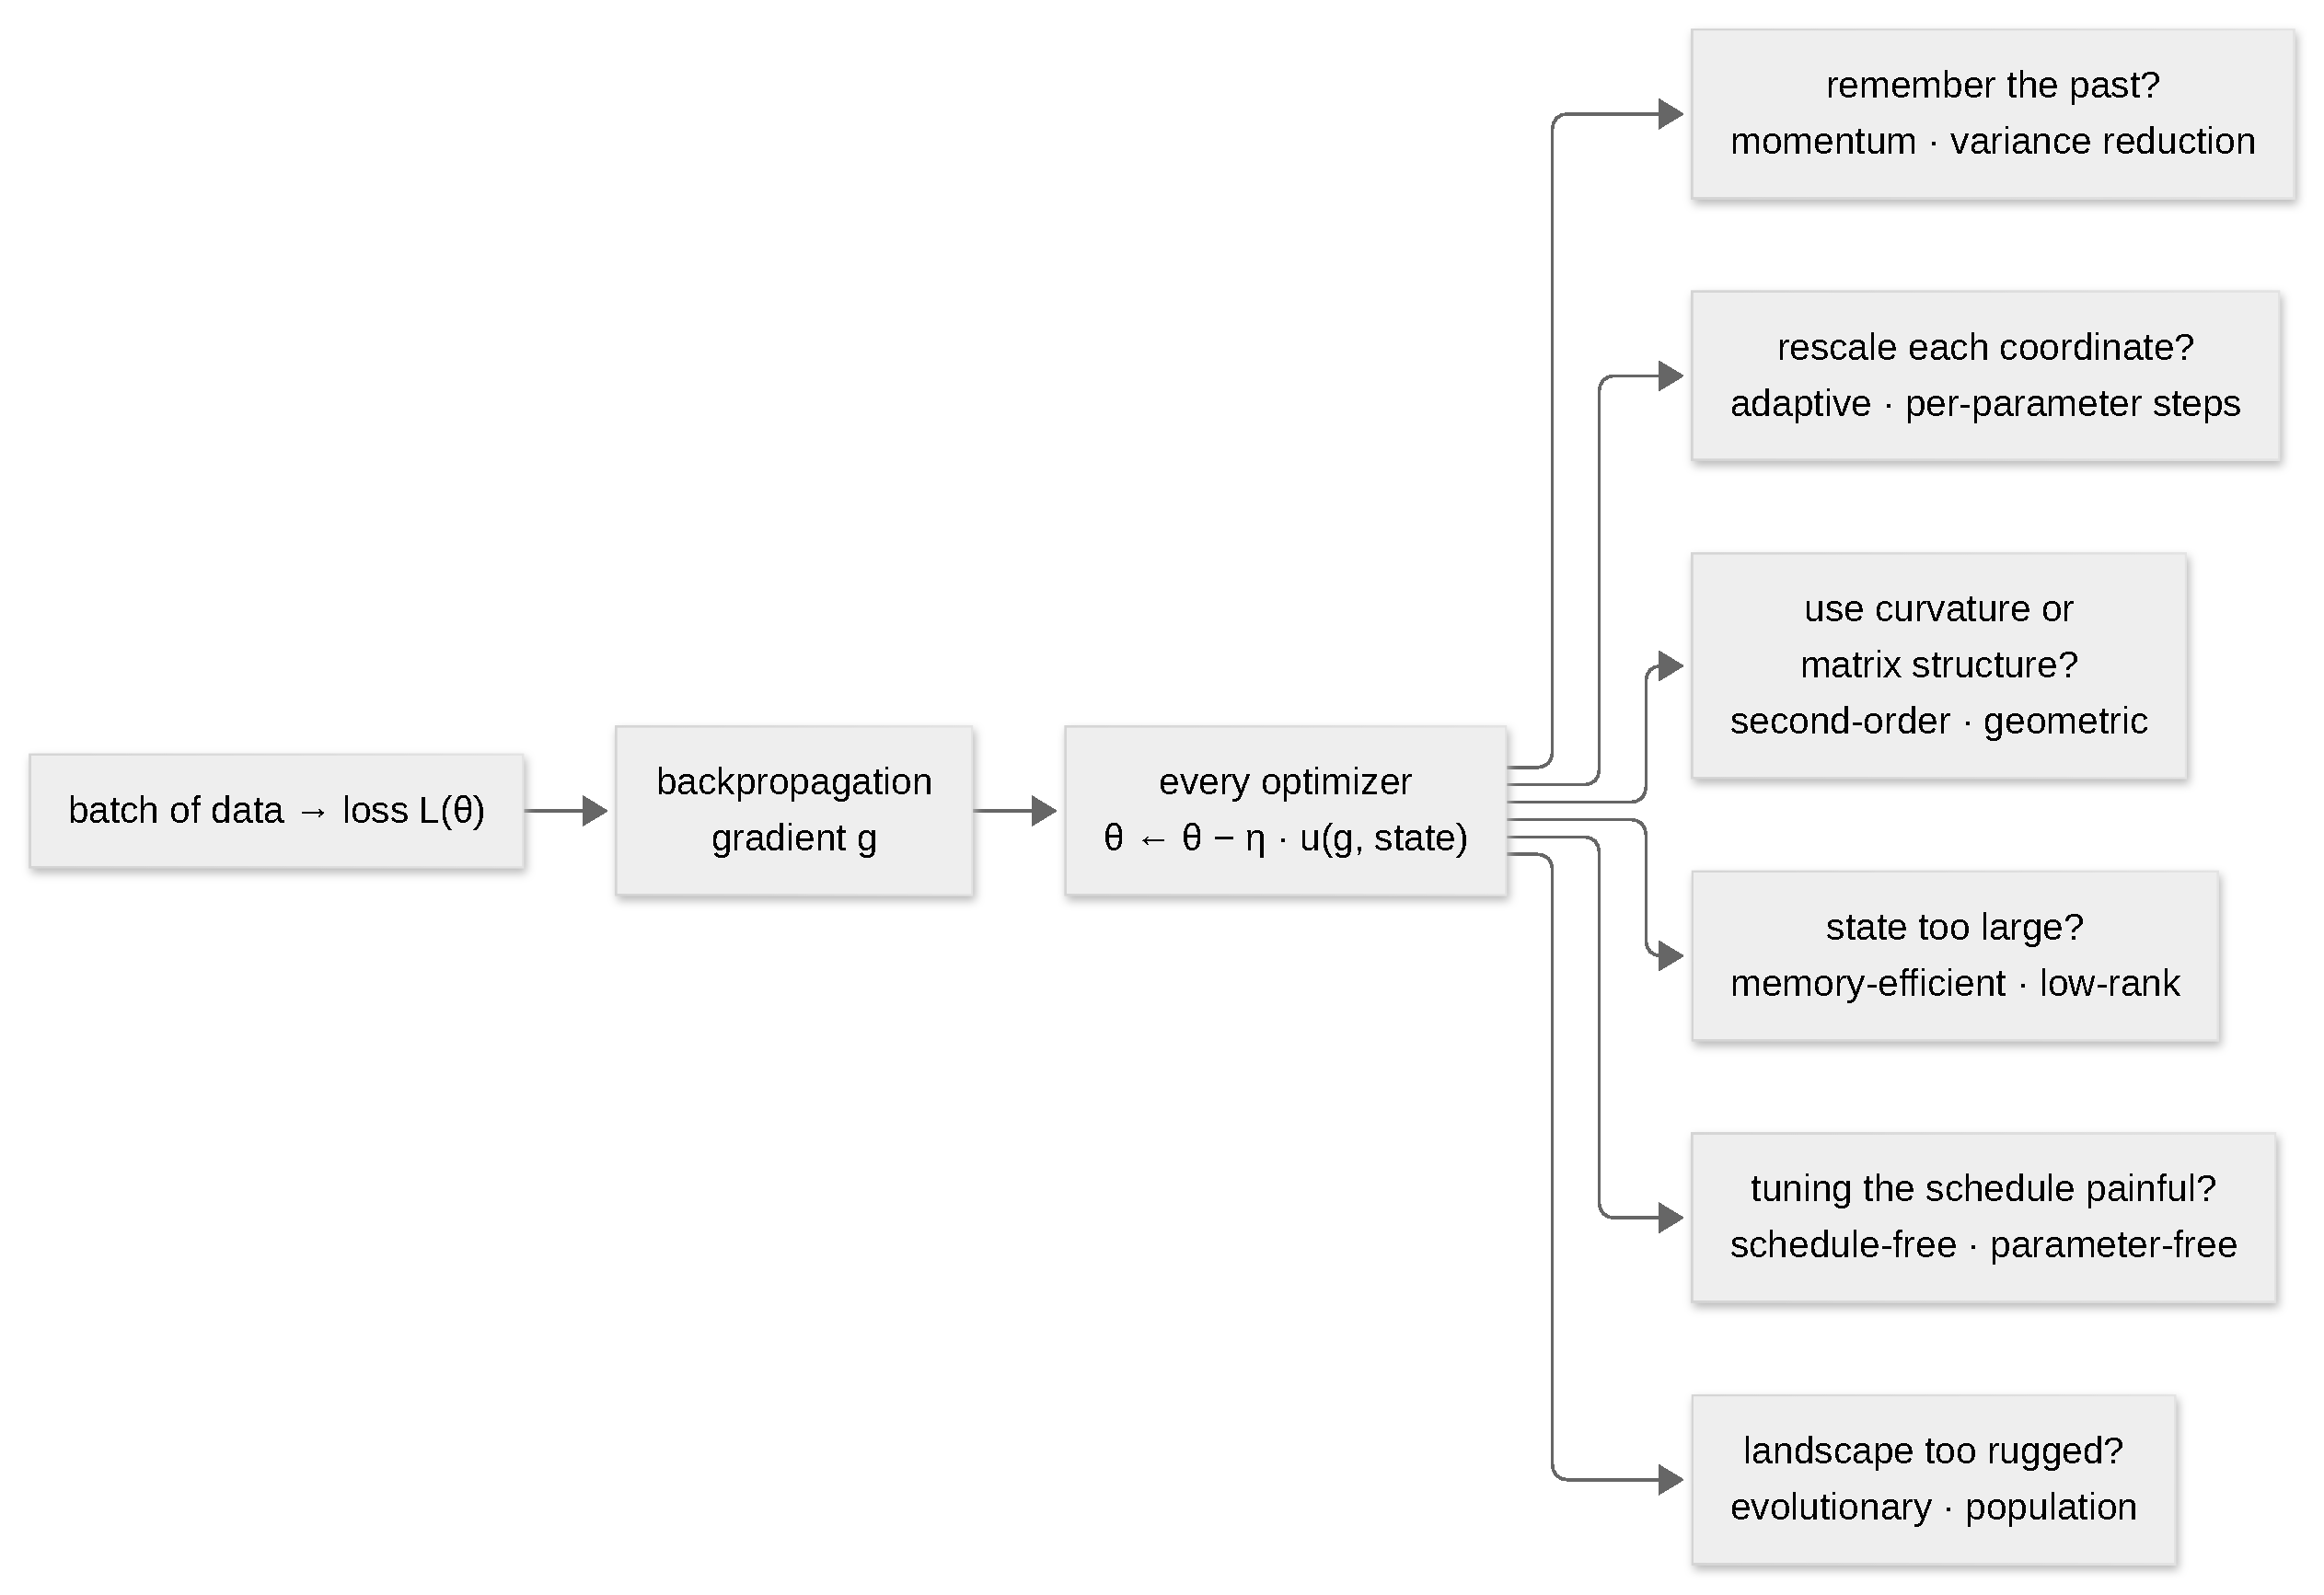
\includegraphics{figures/optimizer-tutorial-flow.pdf}}
\caption{The whole appendix on one page. Data produces a loss, backpropagation
turns the loss into a gradient, and every optimizer applies the same update
rule with a different answer to one of six questions. The questions are
independent, which is why methods can be combined; they are also the only
dimension on which the families in
Section~\ref{sec:annex-optimizers} differ.}
\label{fig:opt-tut-flow}
\end{figure}

\subsubsection{Gradient descent: walk downhill}
\label{sec:opt-tutorial-gd}

For a single weight $w$, the derivative $f'(w)$ is the slope: positive means
the loss grows to the right, so the useful move is to the left. In several
dimensions the gradient $\nabla f$ collects all partial derivatives and points
in the direction of steepest increase; its negative is the direction of
steepest decrease. Taking a step of length $\eta$ along it gives
\begin{equation}
\theta_{t+1} = \theta_t - \eta\,\nabla f(\theta_t),
\label{eq:opt-tut-gd}
\end{equation}
the oldest algorithm in the appendix, usually credited to Cauchy in the
nineteenth century and analysed by Curry in 1944~\citep{ghojogh_ghodsi_2024}. The scalar $\eta>0$ is the
\emph{learning rate} or step size, and it is the only tunable number.

Two facts explain almost everything that follows. First, the step size has a
hard ceiling. If the gradient changes at most $L$ times faster than the
parameters change (the gradient is \emph{$L$-smooth}), then
\eqref{eq:opt-tut-gd} decreases the loss for $\eta<2/L$ and diverges beyond
it; the safe monotone choice is $\eta\le 1/L$~\citep{ghojogh_ghodsi_2024}.
Second, contour lines of a quadratic loss are ellipses whose axes have very
different lengths, and the negative gradient is perpendicular to the contour
but generally does \emph{not} point at the minimum---except when the ellipses
are circles~\citep{hinton_csc321_2012}. The walk therefore zig-zags across the
steep direction while creeping along the flat one.
Figure~\ref{fig:opt-tut-gd} shows the three regimes on the same bowl, and
Figure~\ref{fig:opt-tut-lr} shows what they look like as a loss curve.

\begin{figure}[H]
\centering
\fitfigure{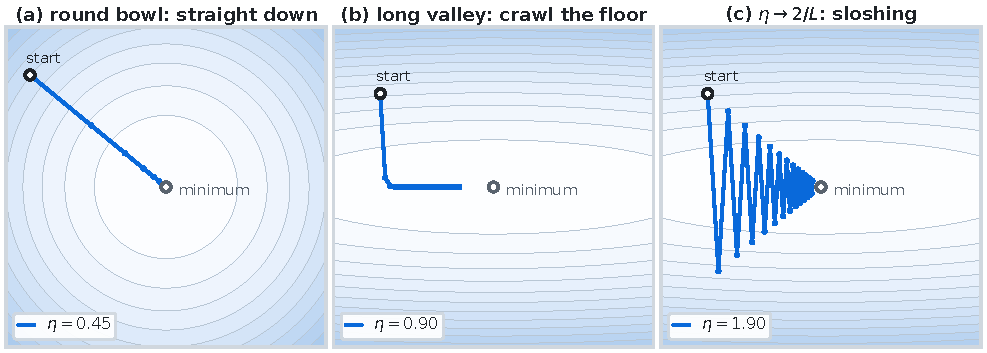
\includegraphics{figures/optimizers/tutorial/tut-gd-landscape.pdf}}
\caption{Gradient descent on a quadratic bowl, same start, 26 steps.
(a) An isotropic bowl: the gradient aims at the minimum and the walk is a
straight line. (b) A valley whose curvature differs by a factor of twenty
between its axes: the steep direction is solved in a few steps, then the walk
crawls along the floor because the same $\eta$ is far too small there.
(c) The same valley with $\eta$ pushed towards the stability limit $2/L$: the
steep direction now alternates sign and the path sloshes. One global step
size cannot serve both directions---the observation that motivates every
per-coordinate method in this appendix~\citep{hinton_csc321_2012}.}
\label{fig:opt-tut-gd}
\end{figure}

\begin{figure}[H]
\centering
\fitfigure{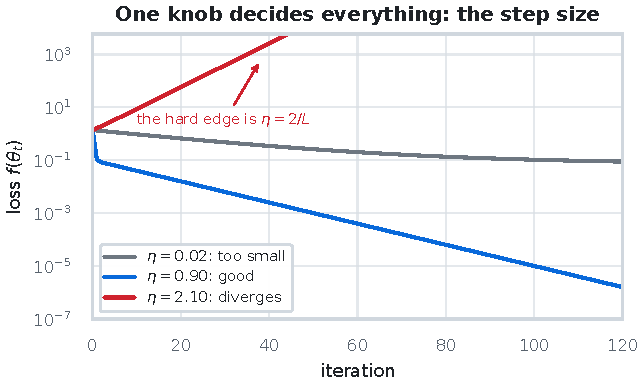
\includegraphics{figures/optimizers/tutorial/tut-learning-rate.pdf}}
\caption{The same valley, one knob. With $\eta$ far below $1/L$ the loss
barely moves; at $\eta\approx1/L$ it falls geometrically; past $\eta=2/L$ every
iteration multiplies the error by a factor larger than one and the run
diverges. The two rates that matter---$1/L$ for monotone decrease and $2/L$
for stability---depend on the curvature, which is exactly what a practitioner
does not know in advance.}
\label{fig:opt-tut-lr}
\end{figure}

When the curvature is unknown, the classical remedy is a \emph{line search}:
try $\eta=1$, halve it until the loss actually decreases, and repeat
\citep{ghojogh_ghodsi_2024}. Deep learning rarely does this, because every
trial costs a full pass over the data; it schedules $\eta$ by hand instead.
Theory supplies the pace: for a convex $L$-smooth objective, gradient descent
reaches $f(\theta_t)-f^\star\le 2L\|\theta_0-\theta^\star\|^2/(t+1)$, that is,
$O(1/t)$~\citep{ghojogh_ghodsi_2024}. Halving the distance to the optimum costs
a doubling of iterations---a fair summary of why first-order methods need so
many steps.

\subsubsection{Where the gradient comes from: backpropagation}
\label{sec:opt-tutorial-backprop}

Nothing above said how to obtain $g_t$. For a network with millions of
weights there is no formula to differentiate by hand, and finite differences
would cost one forward pass per parameter. Backpropagation computes all
partial derivatives in a single backward sweep, using only the chain rule.

In a feed-forward network each layer alternates an affine map and an
activation, $a^{(\ell)}=W^{(\ell)}z^{(\ell-1)}+b^{(\ell)}$ and
$z^{(\ell)}=\sigma(a^{(\ell)})$. The forward pass stores every $a$ and $z$. The
backward pass then propagates one number per neuron,
$\delta^{(\ell)}=\partial e/\partial a^{(\ell)}$, from the loss towards the
input,
\begin{equation}
\delta^{(L)} = \frac{\partial e}{\partial z^{(L)}}\odot\sigma'(a^{(L)}),
\qquad
\delta^{(\ell)} = \sigma'(a^{(\ell)})\odot
\left(W^{(\ell+1)\top}\delta^{(\ell+1)}\right),
\qquad
\frac{\partial e}{\partial W^{(\ell)}} = \delta^{(\ell)}\,z^{(\ell-1)\top},
\label{eq:opt-tut-backprop}
\end{equation}
where $\odot$ is the element-wise product. The gradient of a weight is
therefore the product of a backward number and a forward number---the two
quantities drawn in Figure~\ref{fig:opt-tut-backprop}. The recursion is
linear in the layer index, so the whole sweep costs about the same as one
extra forward pass, roughly twice the forward cost per step, and it must keep
the activations of every layer in memory until they are used
\citep{ghojogh_ghodsi_2024,rumelhart1986learning}.

\begin{figure}[H]
\centering
\fitfigure{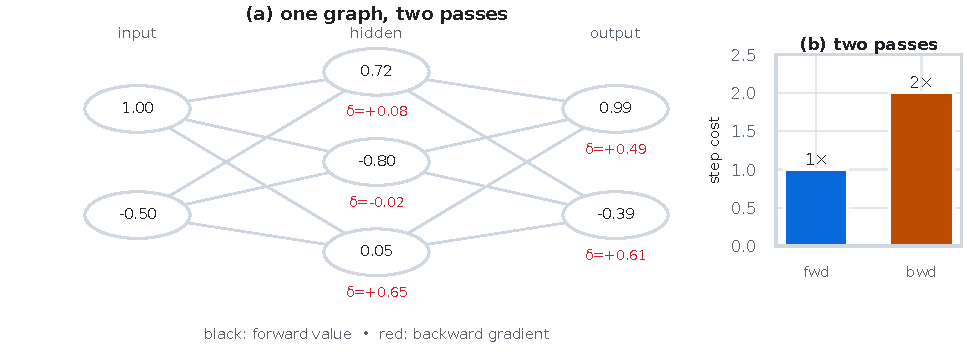
\includegraphics{figures/optimizers/tutorial/tut-backprop.pdf}}
\caption{One training step on a two-hidden-layer network with exact values.
Black numbers are the forward activations $z$; red numbers are the backward
quantities $\delta=\partial e/\partial a$. Every weight gradient is the
product of one red and one black number (equation~\ref{eq:opt-tut-backprop}),
so one backward sweep yields all of them at once. Panel (b): the backward pass
costs about twice the forward pass and keeps the activations alive, which is
why optimizer memory is not the only memory bill in training.}
\label{fig:opt-tut-backprop}
\end{figure}

\begin{algorithm}[H]
\caption{Backpropagation: the gradient factory}
\label{alg:opt-tut-backprop}
\begin{algorithmic}[1]
\Require Input $x$, target $y$, weights $\{W^{(\ell)},b^{(\ell)}\}_{\ell=1}^{L}$
\Ensure Gradients $\{\partial e/\partial W^{(\ell)}\}_{\ell=1}^{L}$
\State Forward: $z^{(0)}\gets x$; \textbf{for} $\ell=1,\dots,L$ \textbf{do} $a^{(\ell)}\gets W^{(\ell)}z^{(\ell-1)}+b^{(\ell)}$, $z^{(\ell)}\gets\sigma(a^{(\ell)})$
\State Loss: $e \gets \ell(z^{(L)}, y)$
\State $\delta^{(L)} \gets \partial e/\partial z^{(L)} \odot \sigma'(a^{(L)})$
\For{$\ell = L, L-1, \dots, 1$}
    \State $\partial e/\partial W^{(\ell)} \gets \delta^{(\ell)} z^{(\ell-1)\top}$
    \State $\partial e/\partial b^{(\ell)} \gets \delta^{(\ell)}$
    \State $\delta^{(\ell-1)} \gets \sigma'(a^{(\ell-1)})\odot\left(W^{(\ell)\top}\delta^{(\ell)}\right)$
\EndFor
\State \Return all weight gradients
\end{algorithmic}
\end{algorithm}

The important consequence for this appendix is that backpropagation is not an
optimizer. It is a gradient factory, and it always returns the exact gradient
of whatever batch it was given. Every difference between the families that
follow lives after the factory, in how $u_t$ in
\eqref{eq:opt-tut-generic} is formed.

\subsubsection{Stochastic and mini-batch gradient descent}
\label{sec:opt-tutorial-sgd}

With $n$ examples the loss is an average, $f(\theta)=\frac1n\sum_i f_i(\theta)$,
so the exact gradient is an average of $n$ per-example gradients and one step
costs $n$ backward passes. For a dataset of a billion tokens that is
unaffordable, and it is also wasteful: neighbouring examples usually say
almost the same thing about the parameters.

Stochastic gradient descent, in the line of the Robbins--Monro stochastic
approximation~\citep{robbins_monro_1951}, replaces the average by one term,
$\hat g_t=\nabla f_{i_t}(\theta_t)$ with $i_t$ drawn uniformly, giving
\begin{equation}
\theta_{t+1} = \theta_t - \eta_t\,\nabla f_{i_t}(\theta_t).
\label{eq:opt-tut-sgd}
\end{equation}
The estimate is unbiased, $\mathbb{E}[\hat g_t]=g_t$, so on average it points
the right way; its error falls as $\sigma/\sqrt{b}$ when a batch of $b$
examples is used instead of one
\citep{ghojogh_ghodsi_2024,bottou_2010}. Modern libraries call this
\emph{mini-batch} method ``SGD'' and almost never use $b=1$: one pass over the
data (an \emph{epoch}) then contains $\lfloor n/b\rfloor$ updates rather than
one~\citep{ibm_sgd_2025,ghojogh_ghodsi_2024}. Figure~\ref{fig:opt-tut-noise}
shows both faces of the trade: with the same number of steps and the same step
size, small batches wander, and the noise they inject is precisely the
quantity that shrinks as $1/\sqrt{b}$.

\begin{figure}[H]
\centering
\fitfigure{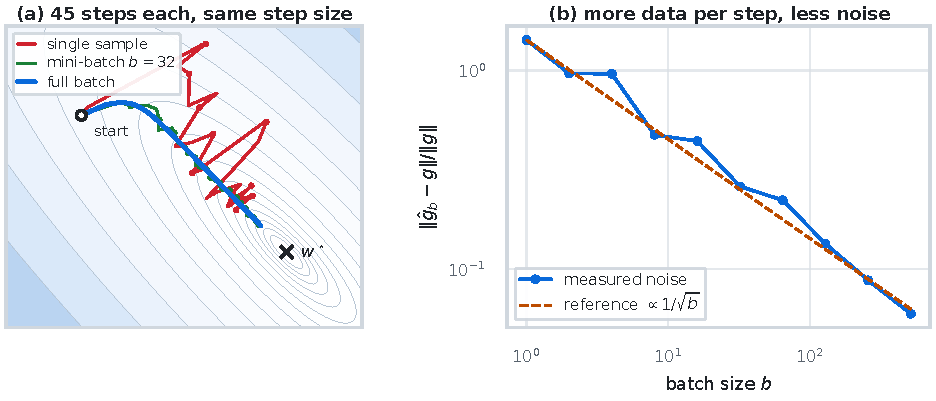
\includegraphics{figures/optimizers/tutorial/tut-batch-noise.pdf}}
\caption{(a) A real least-squares surface in two weights (correlated features,
so the valley is genuine), with 45 steps from the same start and the same step
size. The full batch descends smoothly; a mini-batch of 32 tracks it with a
visible wobble; single-sample gradients never settle. (b) Relative error of
the batch gradient against the full gradient, measured on the same data: the
measured points follow the $1/\sqrt{b}$ law, the noise is halved by
quadrupling the batch.}
\label{fig:opt-tut-noise}
\end{figure}

Noise is not only a cost. Because each step is a random approximation, the
iterate can leave a shallow basin or slide across a saddle that a full-batch
method would treat as a stopping point~\citep{ibm_sgd_2025}. The price appears
in the rate. For a convex $L$-smooth objective, SGD with $\eta_t\propto1/\sqrt
t$ satisfies $f(\theta_t)-f^\star=O(\log t/\sqrt t)$, and with a constant step
it converges to a neighbourhood of size $O(\eta)$ and then
stalls~\citep{ghojogh_ghodsi_2024}. Full-batch gradient descent is therefore
more accurate per iteration and much slower per iteration; SGD is the
opposite. Figure~\ref{fig:opt-tut-rates} puts the two statements on the same
axes, once per iteration and once per unit of wall-clock, which is the
comparison that actually matters when a step costs $n/b$ times less.

\begin{figure}[H]
\centering
\fitfigure{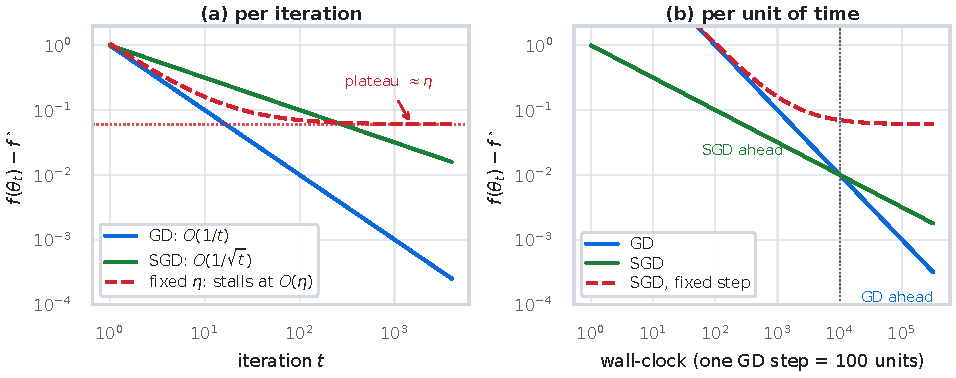
\includegraphics{figures/optimizers/tutorial/tut-convergence.pdf}}
\caption{(a) Per iteration, gradient descent decays as $O(1/t)$ while SGD
decays as $O(1/\sqrt t)$ and, with a fixed step, flattens at a plateau of
height $O(\eta)$~\citep{ghojogh_ghodsi_2024}. The plateau is the reason every
practical recipe eventually reduces $\eta$. (b) The same curves against
wall-clock, with one full-batch step costing a hundred mini-batch steps: SGD
is ahead for most of the run and gradient descent only wins once the plateau
binds. Curves are schematic, with constants chosen for legibility.}
\label{fig:opt-tut-rates}
\end{figure}

\subsubsection{Two knobs that every later method turns}
\label{sec:opt-tutorial-knobs}

Everything after this point is a refinement of two observations about
equation~\eqref{eq:opt-tut-gd}, and it is worth separating them before meeting
the families.

\paragraph{Memory of the past.} A ball rolling down the same valley keeps its
velocity: it accumulates speed along a consistent slope and cancels the
oscillation when the slope keeps changing sign. Momentum implements exactly
that, replacing the gradient by a decaying sum of gradients,
\begin{equation}
v_t = \beta\,v_{t-1} - \eta\,g_t,
\qquad
\theta_{t+1} = \theta_t + v_t,
\label{eq:opt-tut-momentum}
\end{equation}
with $\beta\in[0,1)$ the decay. The effective step is $\eta/(1-\beta)$ along a
steady direction, which is how a small $\eta$ can still move quickly. Nesterov
momentum makes the same move but reads the gradient at the position the
velocity is heading towards, so the correction arrives before the overshoot
does~\citep{hinton_csc321_2012,sutskever2013importance}. Figure
\ref{fig:opt-tut-momentum} shows the composition of the two terms and its
effect on the valley.

\begin{figure}[H]
\centering
\fitfigure{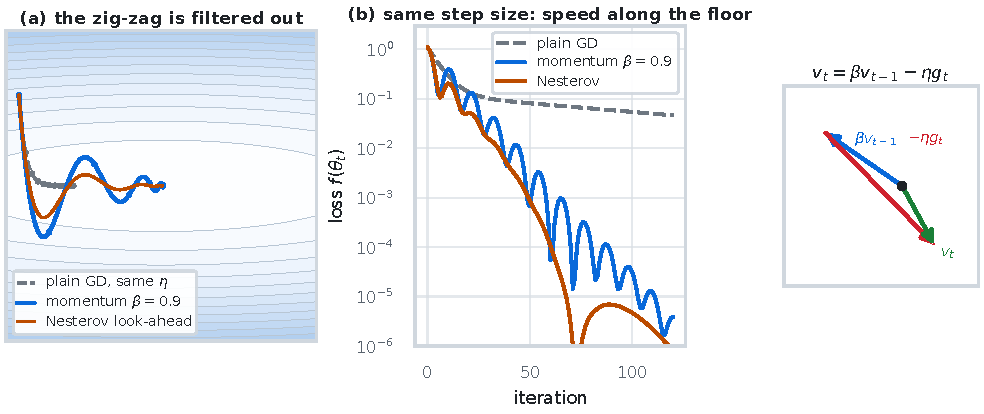
\includegraphics{figures/optimizers/tutorial/tut-momentum.pdf}}
\caption{Momentum as memory. (a) On the valley of
Figure~\ref{fig:opt-tut-gd}(b), with the same step size, plain gradient
descent still crawls along the floor after 120 steps while momentum and its
Nesterov variant reach the minimum. (b) The same run as a loss curve: the
remembered direction buys roughly an order of magnitude. (c) The update is the
head-to-tail sum of the decayed velocity (blue) and the fresh gradient step
(red); the result (green) is smoother than either term alone.}
\label{fig:opt-tut-momentum}
\end{figure}

\paragraph{One step size per coordinate.} The second observation is that the
valley of Figure~\ref{fig:opt-tut-gd}(b) has no single good $\eta$: what is
stable along the steep axis is negligible along the flat one. Adaptive
methods keep a running average of squared gradients and divide by its square
root, so a coordinate that has been receiving large gradients gets a smaller
step and a quiet coordinate gets a larger one,
\begin{equation}
s_t = \gamma\,s_{t-1} + (1-\gamma)\,g_t^2,
\qquad
\theta_{t+1} = \theta_t - \eta\,\frac{g_t}{\sqrt{s_t}+\epsilon}.
\label{eq:opt-tut-rms}
\end{equation}
The scheme grew out of rprop, which used only the sign of the gradient, and
its mini-batch version, rmsprop~\citep{hinton_csc321_2012,tieleman_hinton2012};
AdaGrad is the cumulative rather than decaying version~\citep{duchi_adagrad_2011}.
Figure~\ref{fig:opt-tut-adaptive} shows the effect: the two axes of the valley
receive comparable displacements, at the cost of a per-coordinate state and a
step that no longer shrinks on its own---the residual jitter of size
$\approx\eta$ around the minimum is what later motivates decaying or
schedule-free step sizes.

\begin{figure}[H]
\centering
\fitfigure{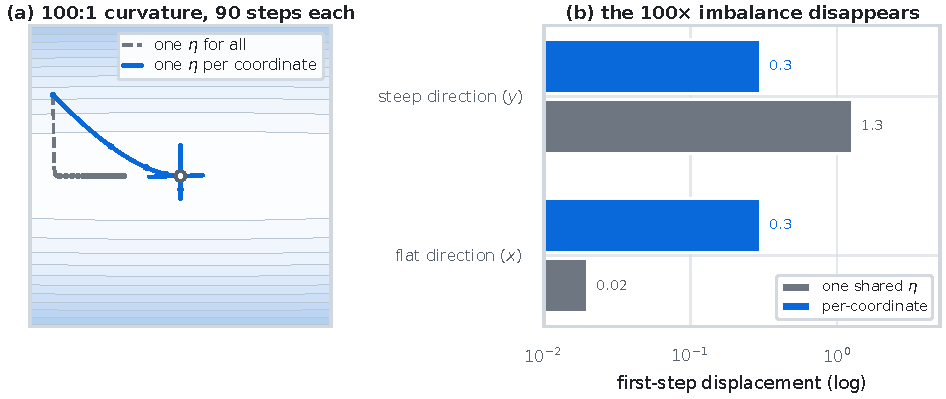
\includegraphics{figures/optimizers/tutorial/tut-adaptive.pdf}}
\caption{One step size per coordinate. (a) On a valley with a hundred-to-one
curvature ratio, a shared step size either overshoots the steep axis or
ignores the flat one; normalising each coordinate by the root-mean-square of
its recent gradients reaches the basin and jitters around it. (b) First-step
displacement per coordinate, on a logarithmic axis: the shared step size
produces a factor of sixty between the axes, the normalised one produces
none.}
\label{fig:opt-tut-adaptive}
\end{figure}

The two knobs compose, and their composition is the reason AdamW is the
default in practice: a first moment for direction, a second moment for scale,
a bias correction for the empty first steps, and a decoupled weight decay for
regularisation~\citep{kingma_adam_2014}. Nothing in
equations~\eqref{eq:opt-tut-momentum} and~\eqref{eq:opt-tut-rms} is specific to
transformers; what differs across the families is which statistics are kept,
how they are combined, and how many bytes per parameter that costs. A compact
survey of the resulting zoo is given by \citet{ruder_2016}.

\subsubsection{How the families differ}
\label{sec:opt-tutorial-families}

The appendix that follows contains thirty-eight methods, which is too many to
hold in mind at once. They are easier to remember as eight families, each
answering one of the questions in Figure~\ref{fig:opt-tut-flow} and each
distinguished by what it remembers and what it pays.

\begin{itemize}[leftmargin=*]
\item \textbf{First-order baselines} (SGD with momentum, AdamW, RAdam) keep one
or two statistics per parameter and assume the landscape is smooth enough for
a locally linear model. They are the reference against which everything else
is measured.
\item \textbf{Momentum and variance reduction} (Adan, ADOPT, AdEMAMix, MARS,
Cautious AdamW) keep more than two buffers, or a gradient difference, to
reduce the variance of the update itself. They buy stability and speed at the
cost of memory and of a second gradient evaluation or a longer history.
\item \textbf{Memory-efficient and low-rank} (Adafactor, GaLore, APOLLO, Lion,
AdamPM) accept a worse estimate of the second moment---a factored one, a
projected one, or none---precisely to shrink the state. Lion goes as far as
keeping only the sign of the update.
\item \textbf{Schedule-free and parameter-free} (Schedule-Free AdamW,
Prodigy, LAMB for large batches) move the burden of choosing $\eta_t$ from the
practitioner to the algorithm, usually by averaging iterates or by estimating
the step from the loss itself.
\item \textbf{Curvature and second-order} (Sophia, Shampoo, SOAP) estimate how
the gradient changes, not just its size, and precondition the step with that
estimate. They converge in fewer iterations and cost more per iteration.
\item \textbf{Geometric and orthogonality} (Muon, Turbo-Muon, AF-Muon, ROOT,
NorMuon, Dion3) treat a weight matrix as a matrix: they orthogonalise or
otherwise whiten the update so that all singular directions move at the same
rate, which is a cheap surrogate for curvature on matrix-shaped parameters.
\item \textbf{Adaptivity-tunable} (Anon) keeps the standard state but adapts
its own coefficients, so the amount of adaptivity is a hyperparameter rather
than a fixed design choice.
\item \textbf{Evolutionary and population} (EvE, EA4LLM) do not follow a
gradient at all: they sample perturbations or maintain a population of models,
which is attractive when gradients are noisy, unavailable, or when many
hyperparameters must be tuned at once, and expensive when the model is large.
\end{itemize}

Table~\ref{tab:opt-tut-families} states the same comparison in the two
currencies that decide a real training run: what is stored per parameter and
what each step costs. Figure~\ref{fig:opt-tut-families} turns it into a
fingerprint: reading down a row tells you which ingredients a family uses,
reading across a column tells you which families share one.

\begin{table}[H]
\centering
\caption{The eight families by the question they answer and what they cost.
State is approximate, in floats per parameter; $k$ is a rank or block count,
$P$ a population size. No family is uniformly better: each line is a trade.}
\label{tab:opt-tut-families}
\small
\begin{tabular}{@{}L{3.2cm}L{4.6cm}L{2.6cm}L{4.6cm}@{}}
\toprule
Family & Question answered & State per parameter & Main risk \\
\midrule
First-order baseline & What is the slope? & 0--2 & needs a hand-tuned schedule \\
Momentum, variance reduction & Which way is it going? & 2--3 & more memory and bookkeeping \\
Memory-efficient, low-rank & Can the state be smaller? & $\le1$ & biased second moment \\
Schedule-free, parameter-free & Can $\eta_t$ be chosen for me? & 1 & theory assumes convexity \\
Curvature, second-order & How does the slope change? & $2+2k$ & expensive factorisations \\
Geometric, orthogonality & Is the update well shaped? & 1 & matrices only \\
Adaptivity-tunable & How adaptive is it? & 2 & extra hyperparameters \\
Evolutionary, population & Can we search without gradients? & $P\times$ & prohibitive at scale \\
\bottomrule
\end{tabular}
\end{table}

\begin{figure}[H]
\centering
\fitfigure{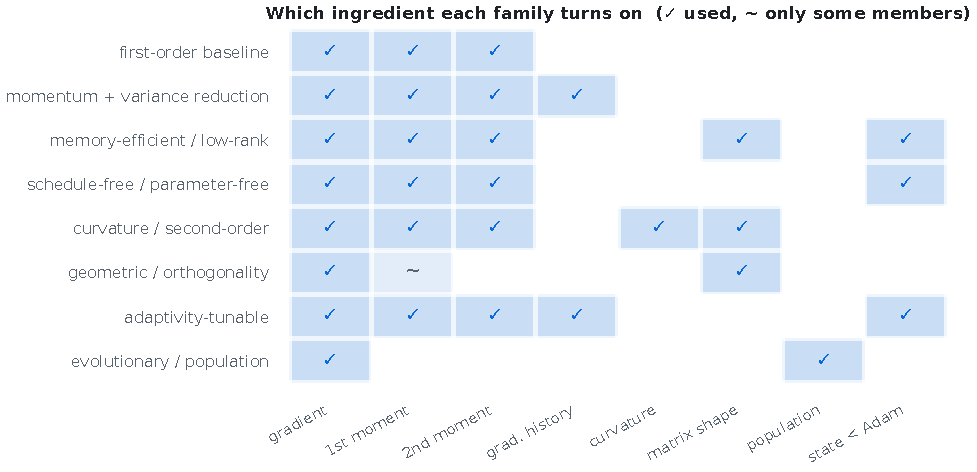
\includegraphics{figures/optimizers/tutorial/tut-families.pdf}}
\caption{A fingerprint of the eight families. A tick marks an ingredient the
family uses, a tilde marks one that only some members use. The first column is
ticked everywhere---every family in this appendix is a gradient method except
the last---and the remaining columns are the actual axes of variation:
direction memory, per-coordinate scale, curvature, matrix structure,
population, and a state smaller than Adam's. The map is deliberately coarse;
the entries that follow give the exact rules.}
\label{fig:opt-tut-families}
\end{figure}

Algorithm~\ref{alg:opt-tut-generic} makes the comparison operational: the
families differ only in which slots they fill. Reading it side by side with
Table~\ref{tab:opt-tut-knobs} is enough to place any method from the rest of
the appendix without memorising its algebra.

\begin{algorithm}[H]
\caption{Any optimizer in this appendix, with the family-specific slots left open}
\label{alg:opt-tut-generic}
\begin{algorithmic}[1]
\Require Parameters $\theta_0$, learning rate $\eta$, slots
$\mathcal{S}$ (state), $\mathcal{D}$ (direction), $\mathcal{P}$ (preconditioner), $\mathcal{T}$ (step rule)
\Ensure Updated parameters $\theta_T$
\State Initialize the state required by $\mathcal{S}$
\For{$t = 1, 2, \ldots, T$}
    \State Sample a batch $\mathcal{B}_t$ and compute $g_t\gets\nabla f_{\mathcal{B}_t}(\theta_{t-1})$ \Comment{backpropagation}
    \State Update the state: $\mathcal{S}\gets\textsc{Update}(\mathcal{S}, g_t, \theta_{t-1})$ \Comment{1st/2nd moment, curvature, population}
    \State Form the direction $u_t\gets\mathcal{D}(g_t,\mathcal{S})$ \Comment{raw gradient, momentum, sign, orthogonalised}
    \State Apply the preconditioner $u_t\gets\mathcal{P}(u_t,\mathcal{S})$ \Comment{per-coordinate scaling, factorised or full}
    \State Choose the step $\eta_t\gets\mathcal{T}(\eta, t, \mathcal{S})$ \Comment{constant, schedule, implicit, self-tuned}
    \State $\theta_t\gets\theta_{t-1}-\eta_t\,u_t$ \Comment{optionally after decoupled weight decay}
\EndFor
\State \Return $\theta_T$
\end{algorithmic}
\end{algorithm}

\begin{table}[H]
\centering
\caption{The slots of Algorithm~\ref{alg:opt-tut-generic} and the knob each one
turns. A method is identified by the slots it fills, not by its name.}
\label{tab:opt-tut-knobs}
\small
\begin{tabular}{@{}L{2.4cm}L{4.4cm}L{3.4cm}L{3.6cm}@{}}
\toprule
Slot & What it decides & Knob turned & Seen in \\
\midrule
$\mathcal{B}_t$ & how many examples per step & variance & SGD, mini-batch, full batch \\
$\mathcal{S}$ & what is remembered & state and memory & momentum, Adam, Sophia, Shampoo \\
$\mathcal{D}$ & which direction is followed & smoothing & momentum, Nesterov, sign methods \\
$\mathcal{P}$ & how coordinates are rescaled & conditioning & AdaGrad, RMSProp, Adam, Muon \\
$\mathcal{T}$ & how long the step is & schedule & cosine, warmup, schedule-free, Prodigy \\
decay & how parameters are regularised & generalisation & L2, decoupled weight decay \\
\bottomrule
\end{tabular}
\end{table}

\subsubsection{Reading a loss curve}
\label{sec:opt-tutorial-diagnostics}

The practical value of the five ideas is diagnostic. A single loss curve
already says which of them is wrong, and the answer is usually visible within
a few hundred steps (Figure~\ref{fig:opt-tut-diag}).

\begin{figure}[H]
\centering
\fitfigure{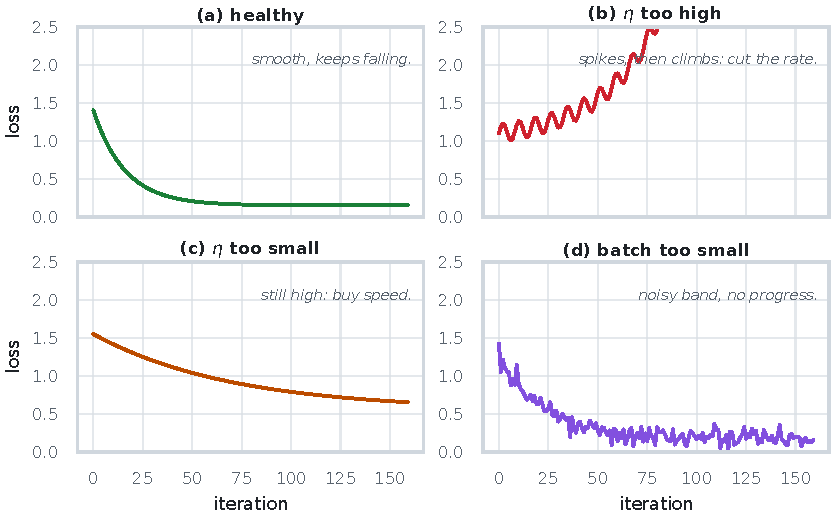
\includegraphics{figures/optimizers/tutorial/tut-loss-diagnostics.pdf}}
\caption{Four loss curves and the sentence each one is saying. A smooth curve
that keeps falling is healthy; spikes followed by a rise mean the step size
crossed $2/L$; a curve that is smooth but far too high means the step size is
far below $1/L$ or the schedule decayed too early; a curve that reaches a
noisy band and stops improving usually means the batch is too small or the
step size has hit its $O(\eta)$ plateau.}
\label{fig:opt-tut-diag}
\end{figure}

Five rules of thumb close the tutorial, all of them consequences of the
figures above rather than of any particular method.
\begin{enumerate}[leftmargin=*]
\item Start from a first-order baseline with both moments (AdamW). It is the
cheapest configuration that survives heterogeneous curvature.
\item If the optimizer state does not fit in memory, change family before
changing hyper parameters: the memory-efficient and low-rank families exist
for exactly that constraint.
\item If tuning the schedule consumes the experiment budget, the schedule-free
and parameter-free families remove the knob instead of tuning it.
\item If most parameters live in matrices (attention and feed-forward
projections), geometric methods exploit a structure that element-wise methods
ignore; if the model is small and the search is over many configurations,
population methods become affordable.
\item Change one slot at a time. Because the families are orthogonal
compositions, a run that changes two of them cannot attribute its result.
\end{enumerate}

The rest of this appendix is the reference behind these statements: one entry
per method, each stating its update rule, its pseudocode, its memory profile,
and the trade it makes.

\subsection{Standard Baseline and Adaptive Optimizers}
\paragraph{SGD with Momentum.}
\begin{figure}[H]
\centering
\fitfigure{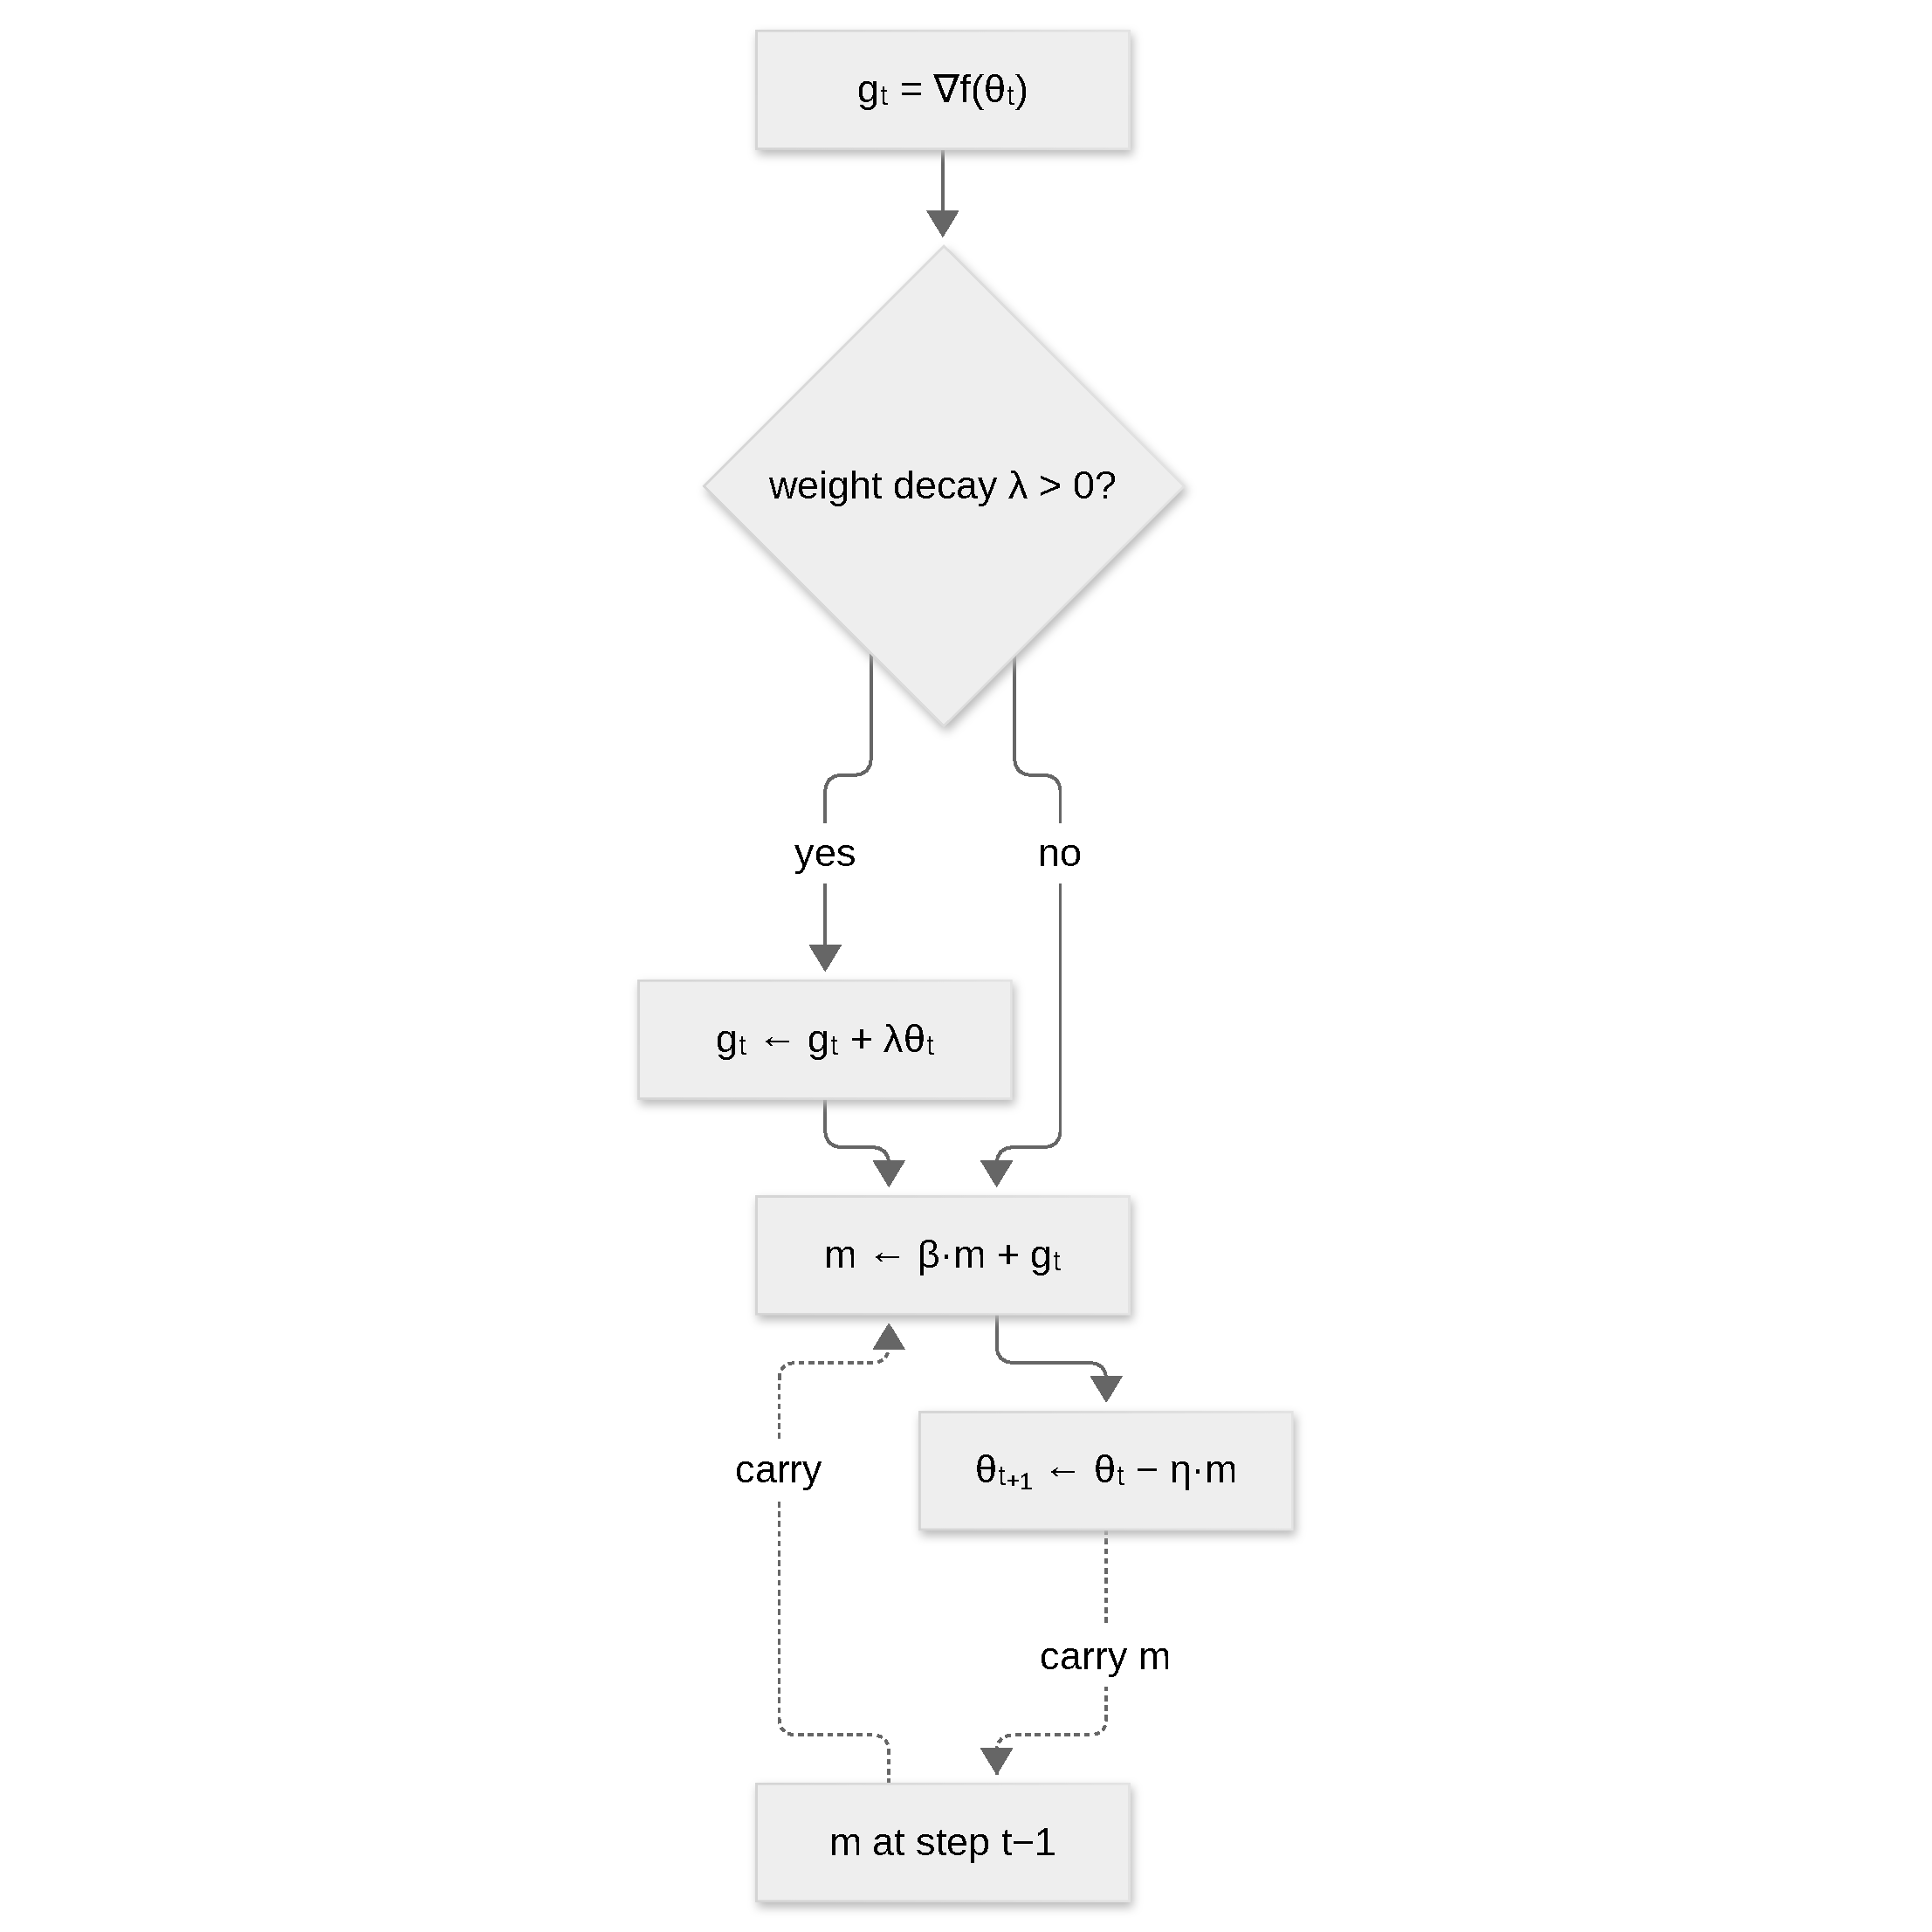
\includegraphics{figures/optimizers/sgd-momentum.pdf}}
\caption{Step flow of SGD with momentum: optional L2 weight decay, exponential momentum accumulation, and the fixed-step parameter update.}
\label{fig:opt-sgd-momentum}
\end{figure}
The classical update accumulates a momentum buffer and then applies a fixed learning rate. At each iteration $t$, the algorithm maintains an exponential moving average $m_t$ of past gradients:
\begin{align}
m_t &= \beta m_{t-1} + g_t \\
\theta_{t+1} &= \theta_t - \eta m_t
\end{align}
where $g_t = \nabla f(\theta_t)$, $\beta \in [0.8, 0.99]$ controls the momentum decay, and $\eta$ is the fixed learning rate. The momentum term acts as velocity: it accelerates movement in consistent directions while dampening oscillations in variable directions.

\begin{algorithm}[H]
\caption{SGD with Momentum}
\label{alg:sgd-momentum}
\begin{algorithmic}[1]
\Require Initial parameters $\theta_0$, learning rate $\eta$, momentum coefficient $\beta$, weight decay $\lambda$
\Ensure Updated parameters $\theta_T$
\State Initialize: momentum buffer $m \gets 0$
\For{$t = 0, 1, 2, \ldots, T-1$}
    \State Compute gradient: $g_t \gets \nabla f(\theta_t)$
    \If{weight\_decay $> 0$}
        \State $g_t \gets g_t + \lambda \theta_t$ \Comment{L2 regularization}
    \EndIf
    \State Update momentum: $m \gets \beta \cdot m + g_t$
    \State Update parameters: $\theta_{t+1} \gets \theta_t - \eta \cdot m$
\EndFor
\Return $\theta_T$
\end{algorithmic}
\end{algorithm}

\paragraph{Cons.}
\begin{itemize}[leftmargin=*]
\item Poor robustness to heterogeneous curvature: a single global rate cannot suit every parameter group.
\item Strong dependence on carefully engineered learning-rate schedules.
\end{itemize}

\paragraph{Pros.}
\begin{itemize}[leftmargin=*]
\item Low memory overhead: a single momentum buffer per parameter.
\item Strong generalization when tuned carefully, and a simple update to implement.
\end{itemize}

\paragraph{Adam and AdamW.}
\begin{figure}[H]
\centering
\fitfigure{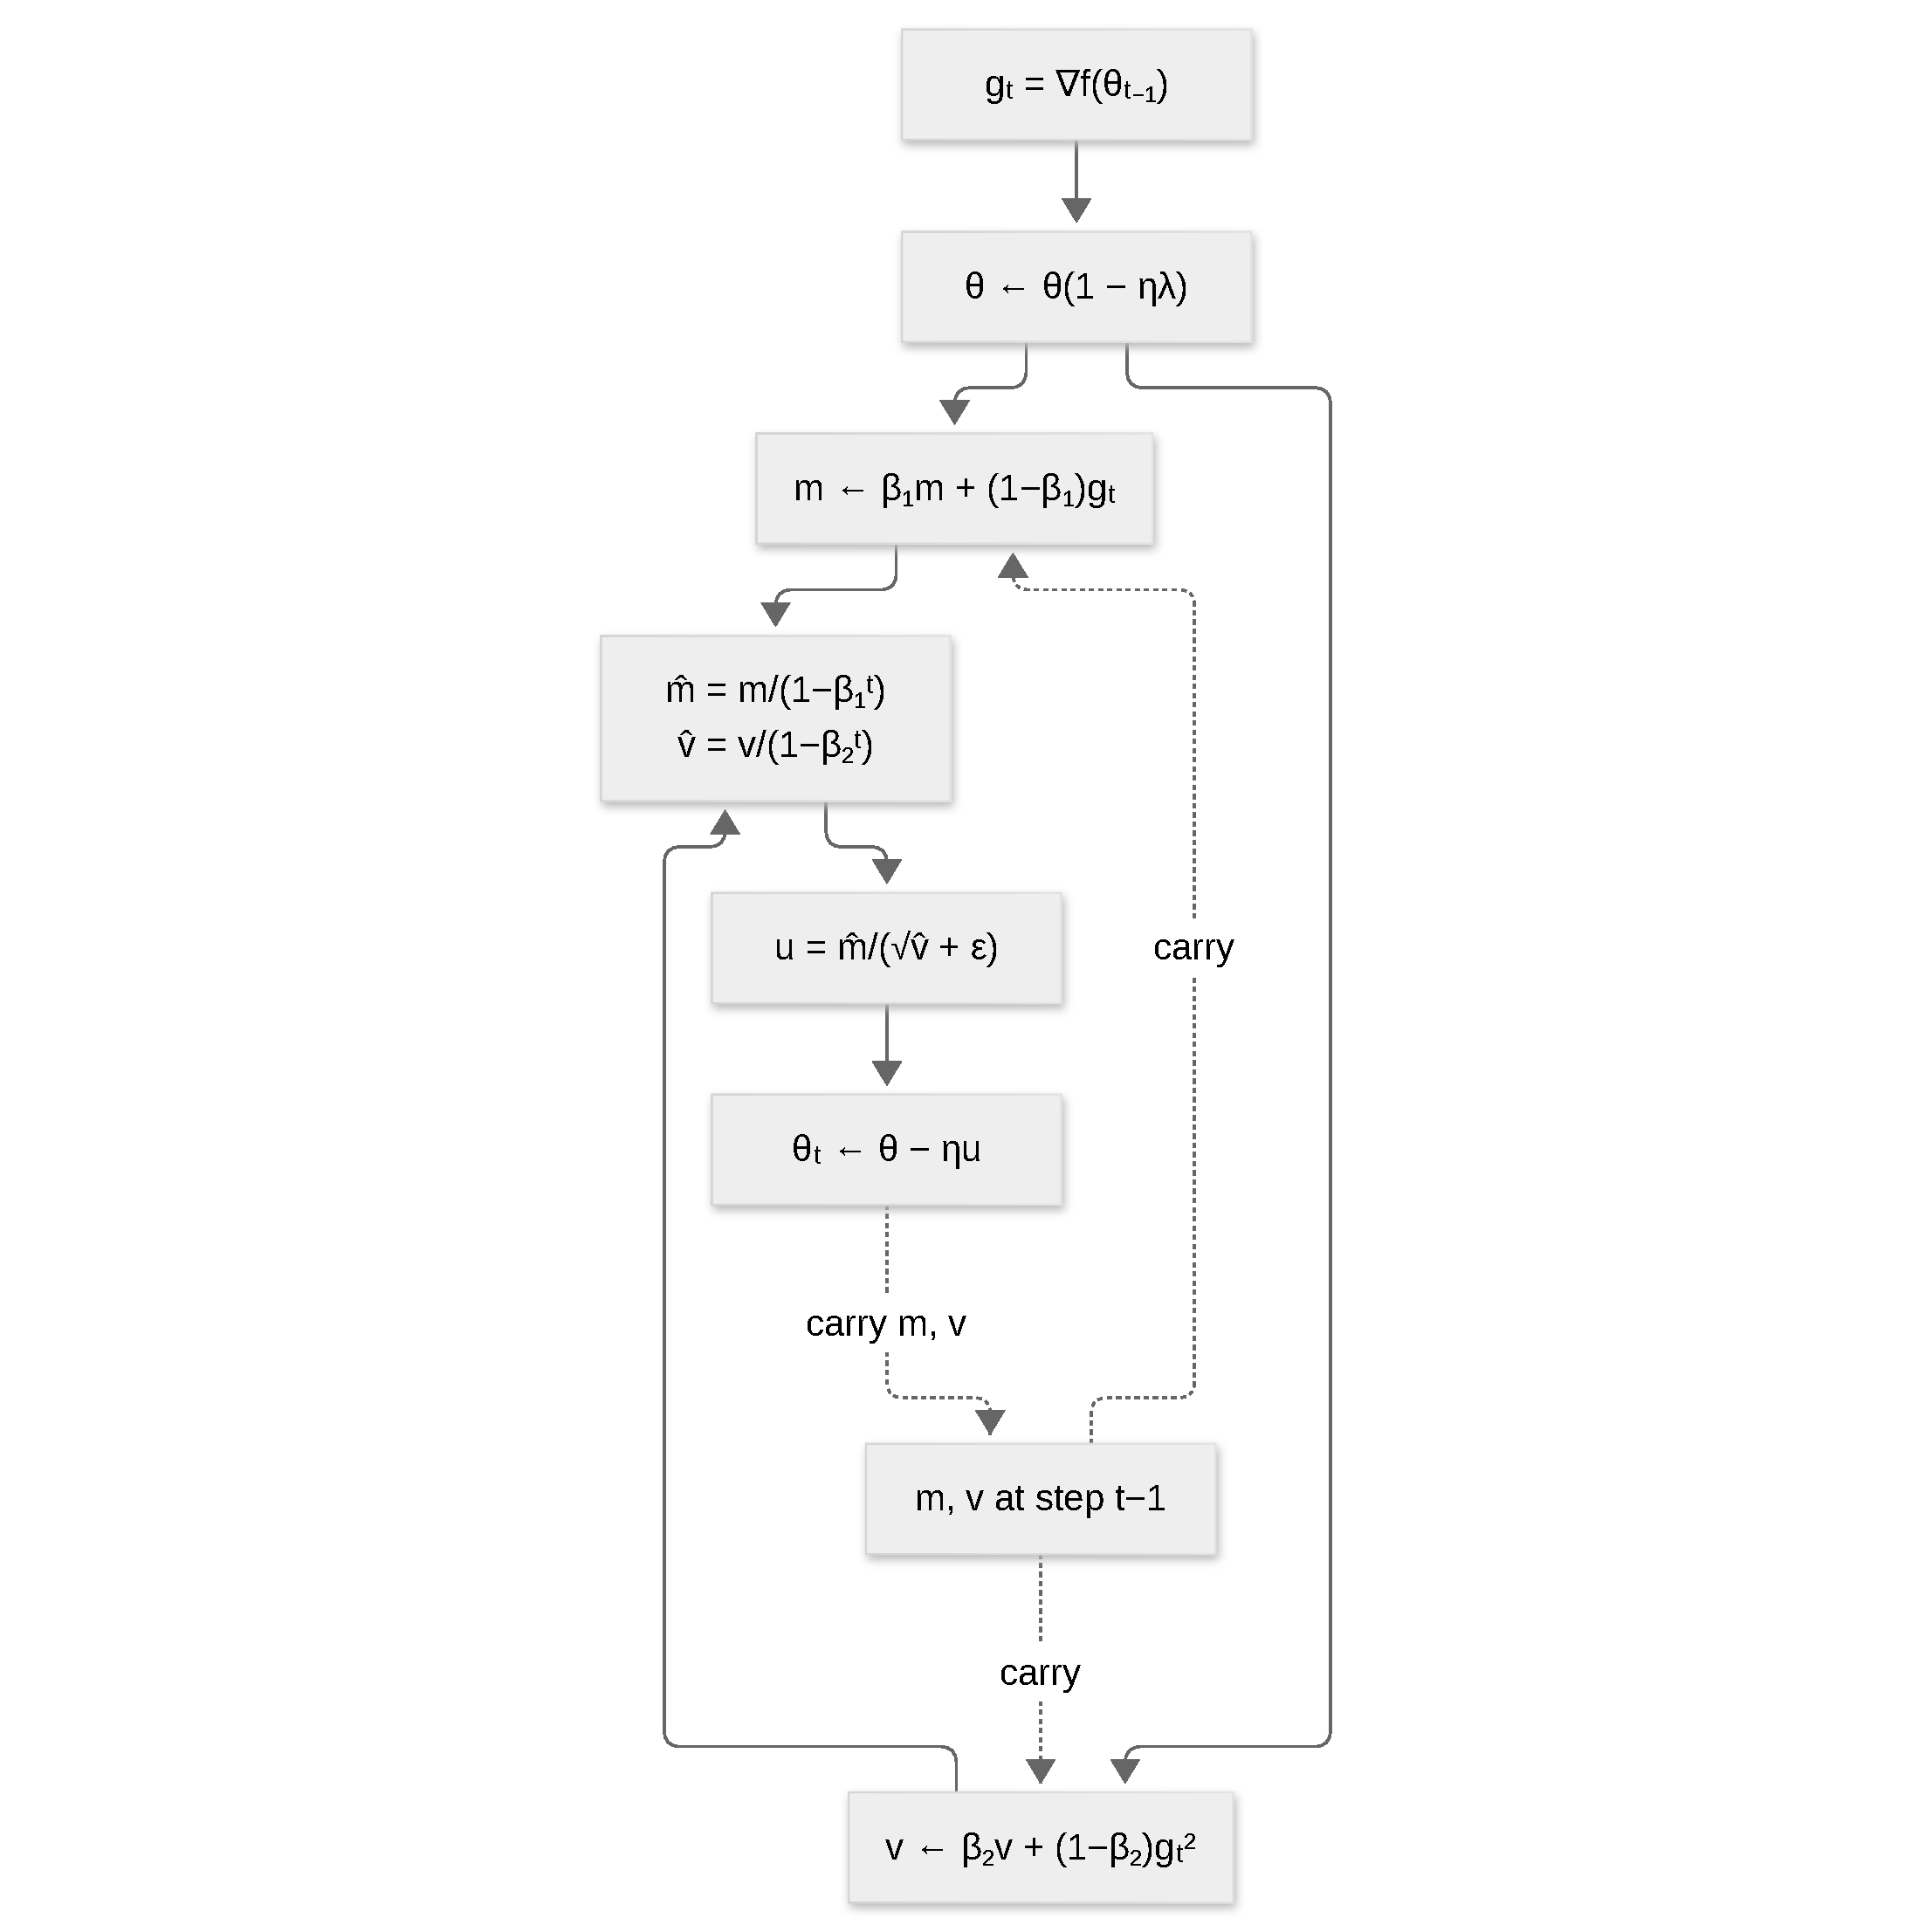
\includegraphics{figures/optimizers/adamw.pdf}}
\caption{Step flow of AdamW: decoupled weight decay, first- and second-moment EMAs, bias correction, and the element-wise adaptive update.}
\label{fig:opt-adamw}
\end{figure}
Adam tracks exponential moving averages of both first moment (mean) and second moment (uncentered variance) to achieve element-wise adaptive learning rates. The update rule is:
\begin{align}
m_t &= \beta_1 m_{t-1} + (1-\beta_1) g_t \\
v_t &= \beta_2 v_{t-1} + (1-\beta_2) g_t^2 \\
\hat{m}_t &= \frac{m_t}{1-\beta_1^t}, \quad \hat{v}_t = \frac{v_t}{1-\beta_2^t} \quad \text{(bias correction)} \\
\theta_{t+1} &= \theta_t - \eta \left(\frac{\hat{m}_t}{\sqrt{\hat{v}_t}+\epsilon}\right)
\end{align}
AdamW introduces a crucial modification: weight decay is applied directly to parameters (decoupled from gradients): $\theta_t \gets \theta_t(1-\eta\lambda)$ rather than adding $\lambda\theta_t$ to the gradient. This decoupling prevents the adaptive scaling from interfering with regularization strength.

\begin{algorithm}[H]
\caption{AdamW (Adam with Decoupled Weight Decay)}
\label{alg:adamw}
\begin{algorithmic}[1]
\Require Initial parameters $\theta_0$, learning rate $\eta$, exponential decay rates $\beta_1, \beta_2 \in [0,1)$
\Require Momentum constant $\epsilon$, weight decay $\lambda$
\Ensure Updated parameters $\theta_T$
\State Initialize: first moment $m \gets 0$, second moment $v \gets 0$, step counter $t \gets 0$
\For{$t = 1, 2, \ldots, T$}
    \State Compute gradient: $g_t \gets \nabla f(\theta_{t-1})$
    \State Weight decay (decoupled): $\theta_{t-1} \gets \theta_{t-1}(1 - \eta\lambda)$
    \State Update moments: $m \gets \beta_1 m + (1-\beta_1) g_t$
    \State $v \gets \beta_2 v + (1-\beta_2) g_t^2$
    \State Bias correction: $\hat{m} \gets m / (1 - \beta_1^t)$, $\hat{v} \gets v / (1 - \beta_2^t)$
    \State Update parameters: $\theta_t \gets \theta_{t-1} - \eta (\hat{m} / (\sqrt{\hat{v}} + \epsilon))$
\EndFor
\Return $\theta_T$
\end{algorithmic}
\end{algorithm}

\paragraph{Cons.}
\begin{itemize}[leftmargin=*]
\item Stores first and second moment tensors for every parameter, doubling optimizer-state memory relative to SGD.
\item Element-wise adaptive scaling can interfere with regularization unless weight decay is decoupled.
\end{itemize}

\paragraph{Pros.}
\begin{itemize}[leftmargin=*]
\item Practical baseline for transformer fine-tuning: fast convergence and forgiving to hyperparameter variation.
\item Decoupled weight decay keeps the regularization strength independent of the adaptive scaling.
\end{itemize}

\paragraph{RAdam (Rectified Adam).}
\begin{figure}[H]
\centering
\fitfigure{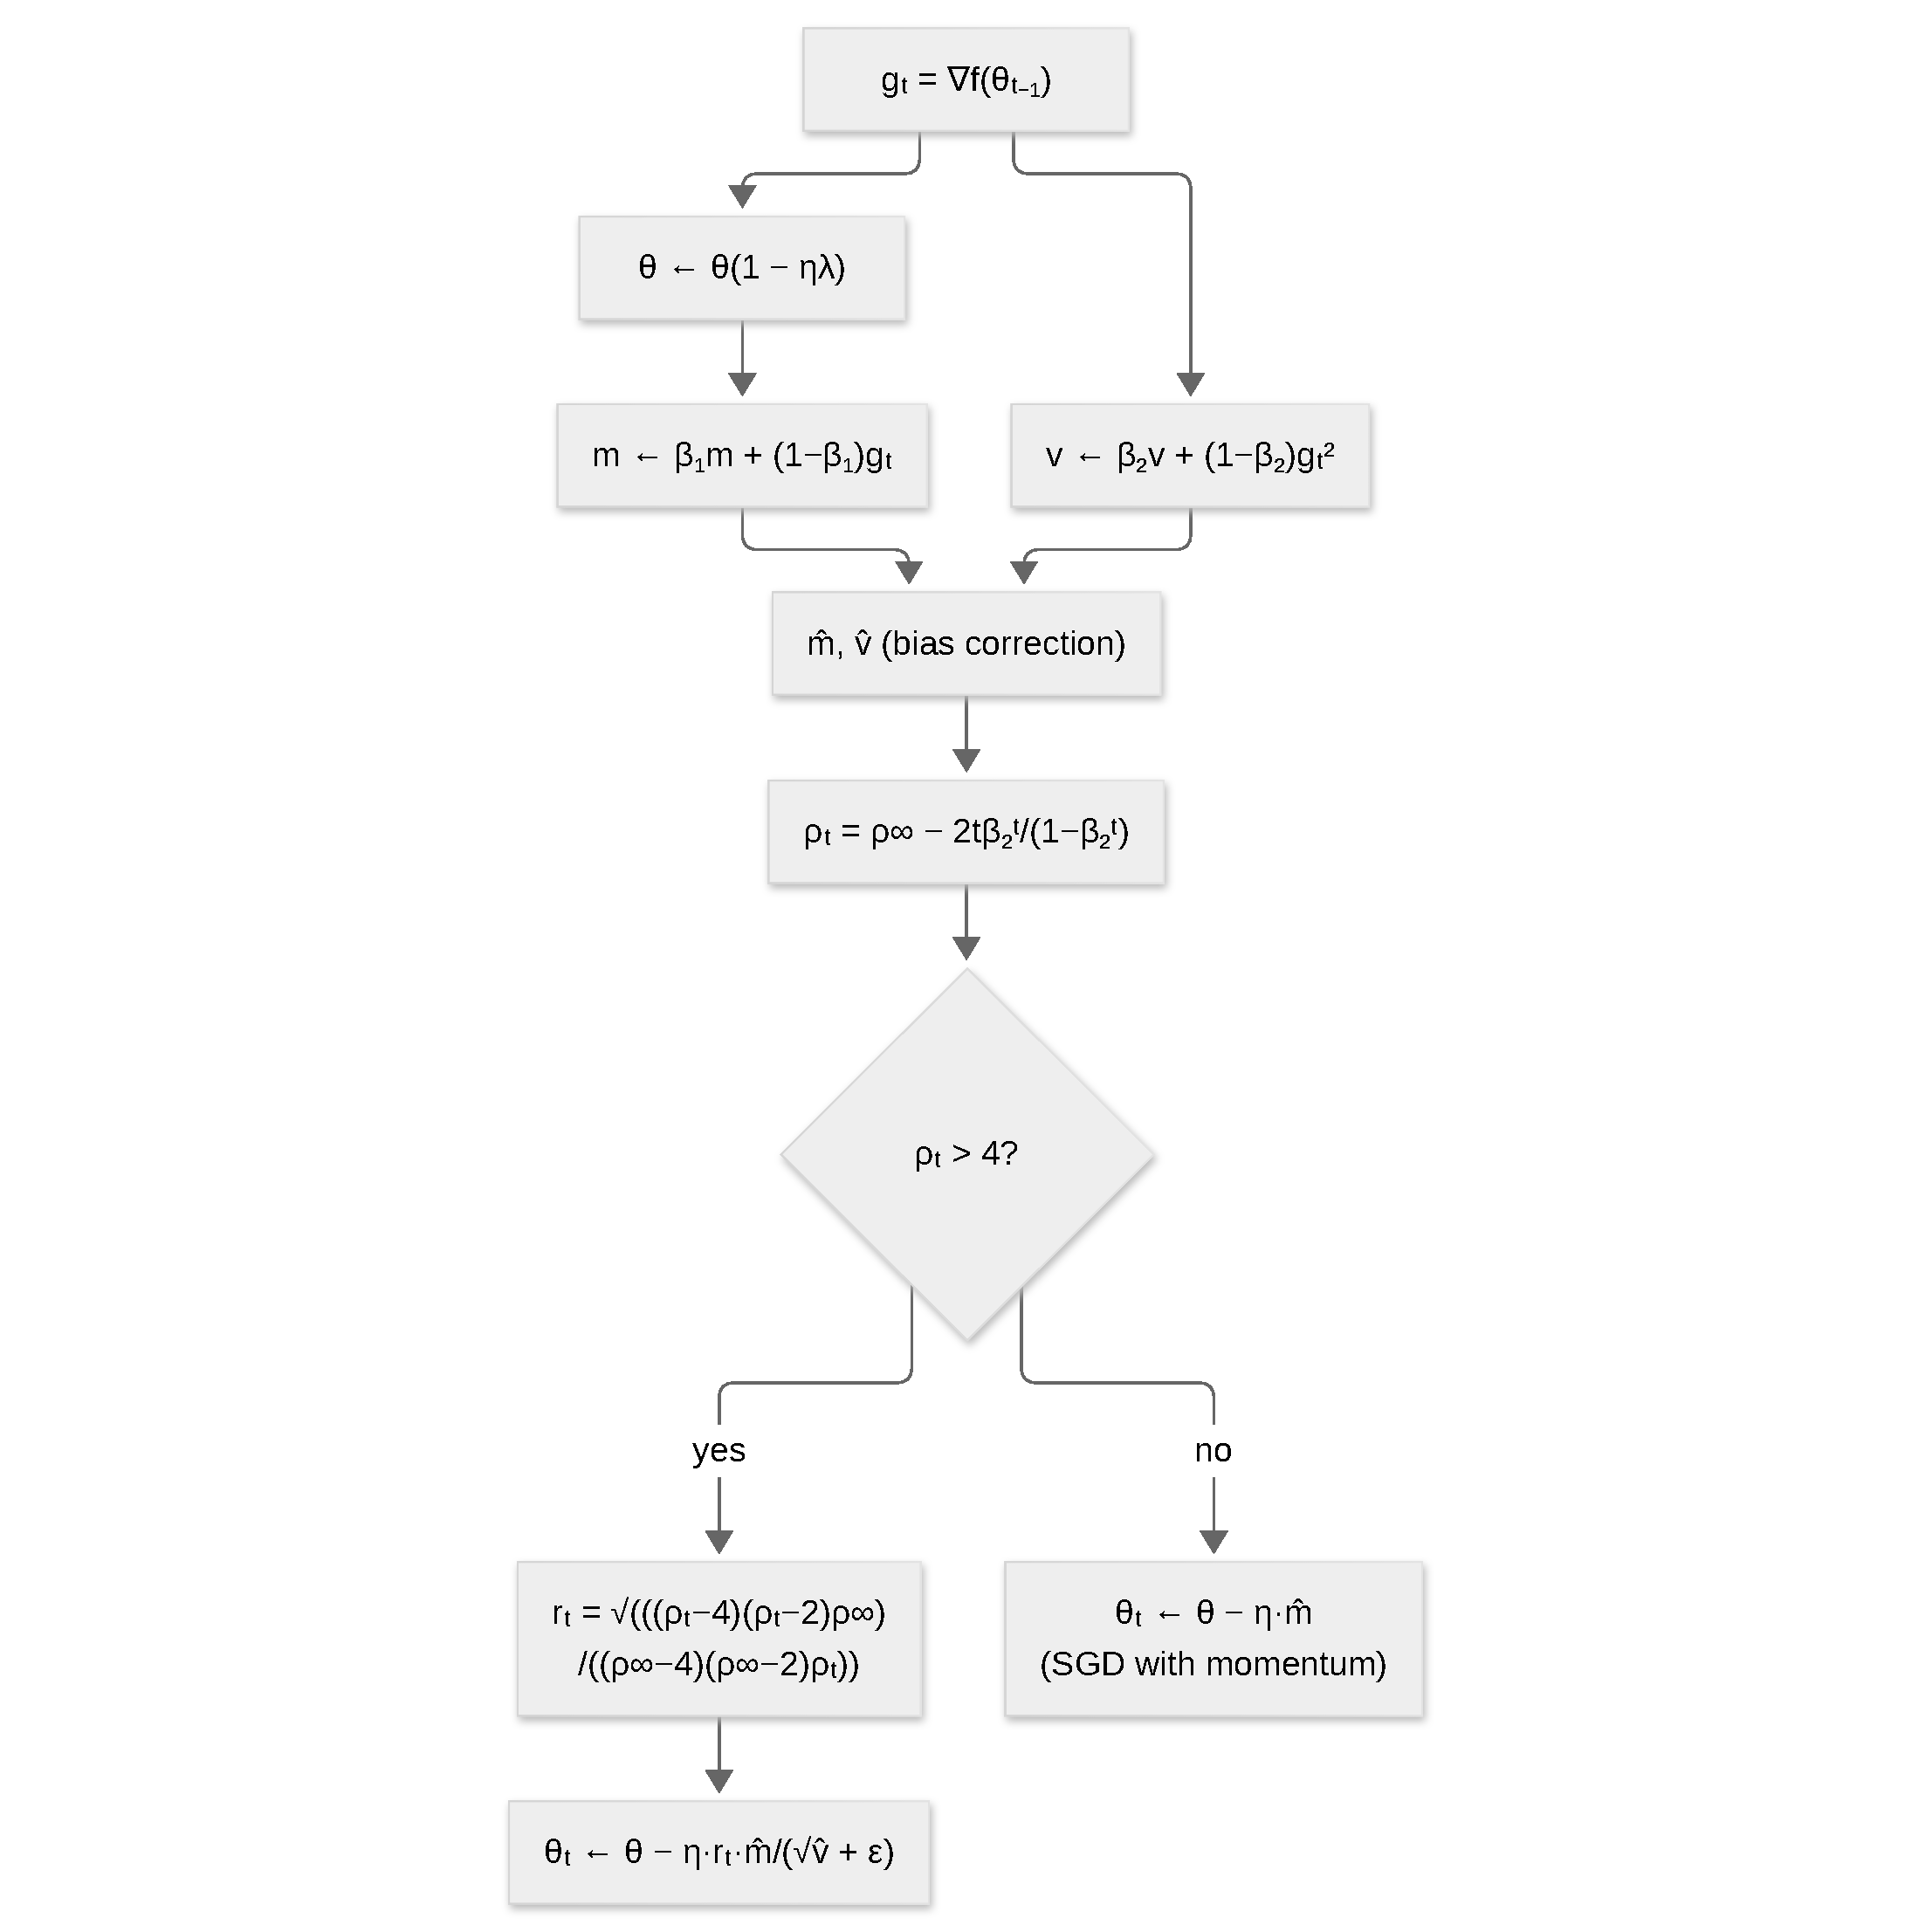
\includegraphics{figures/optimizers/radam.pdf}}
\caption{Step flow of RAdam: SMA-window rectification with an early-step fallback to momentum SGD.}
\label{fig:opt-radam}
\end{figure}
RAdam addresses Adam's instability in early training by dynamically rectifying the adaptive learning rate. The key observation is that the second moment $v_t$ has very high variance in the first few steps, causing unreliable adaptive scaling. RAdam computes the effective simple moving average (SMA) window length:
\[\rho_t = \rho_{\infty} - \frac{2t\beta_2^t}{1-\beta_2^t}, \quad \text{where} \quad \rho_{\infty} = \frac{2}{1-\beta_2}-1\]
When $\rho_t > 4$ (sufficient samples for variance estimation), RAdam applies adaptive scaling with a rectification term:
\[r_t = \sqrt{\frac{(\rho_t-4)(\rho_t-2)\rho_{\infty}}{(\rho_{\infty}-4)(\rho_{\infty}-2)\rho_t}}, \quad \theta_{t+1} = \theta_t - \eta r_t \frac{\hat{m}_t}{\sqrt{\hat{v}_t}+\epsilon}\]
When $\rho_t \leq 4$, RAdam falls back to SGD with momentum: $\theta_{t+1} = \theta_t - \eta\hat{m}_t$.

\begin{algorithm}[H]
\caption{RAdam (Rectified Adam)}
\label{alg:radam}
\begin{algorithmic}[1]
\Require Initial parameters $\theta_0$, learning rate $\eta$, $\beta_1, \beta_2$, weight decay $\lambda$
\Ensure Updated parameters $\theta_T$
\State Initialize: $m \gets 0$, $v \gets 0$, $t \gets 0$
\State Compute: $\rho_\infty \gets 2/(1-\beta_2) - 1$
\For{$t = 1, 2, \ldots, T$}
    \State $g_t \gets \nabla f(\theta_{t-1})$
    \If{weight\_decay $> 0$}
        \State $\theta_{t-1} \gets \theta_{t-1}(1 - \eta\lambda)$
    \EndIf
    \State $m \gets \beta_1 m + (1-\beta_1) g_t$
    \State $v \gets \beta_2 v + (1-\beta_2) g_t^2$
    \State $\hat{m} \gets m/(1-\beta_1^t)$, $\hat{v} \gets v/(1-\beta_2^t)$
    \State $\rho_t \gets \rho_\infty - 2t \beta_2^t / (1 - \beta_2^t)$
    \If{$\rho_t > 4$}
        \State $r_t \gets \sqrt{((\rho_t-4)(\rho_t-2)\rho_\infty) / ((\rho_\infty-4)(\rho_\infty-2)\rho_t)}$
        \State $\theta_t \gets \theta_{t-1} - \eta r_t \hat{m} / (\sqrt{\hat{v}} + \epsilon)$
    \Else
        \State $\theta_t \gets \theta_{t-1} - \eta \hat{m}$ \Comment{SGD with momentum}
    \EndIf
\EndFor
\Return $\theta_T$
\end{algorithmic}
\end{algorithm}

\paragraph{Cons.}
\begin{itemize}[leftmargin=*]
\item Adds rectification bookkeeping on top of Adam's moment state.
\item The benefit shrinks when a well-tuned warmup schedule is already in use.
\end{itemize}

\paragraph{Pros.}
\begin{itemize}[leftmargin=*]
\item Eliminates the need for manual learning-rate warmup by rectifying the adaptive rate.
\item Falls back gracefully to momentum SGD while variance estimates are unreliable, improving robustness.
\end{itemize}


\subsection{Advanced Momentum and Variance Reduction (2024--2025)}
\paragraph{Adan (Adaptive Nesterov Momentum).}
\begin{figure}[H]
\centering
\fitfigure{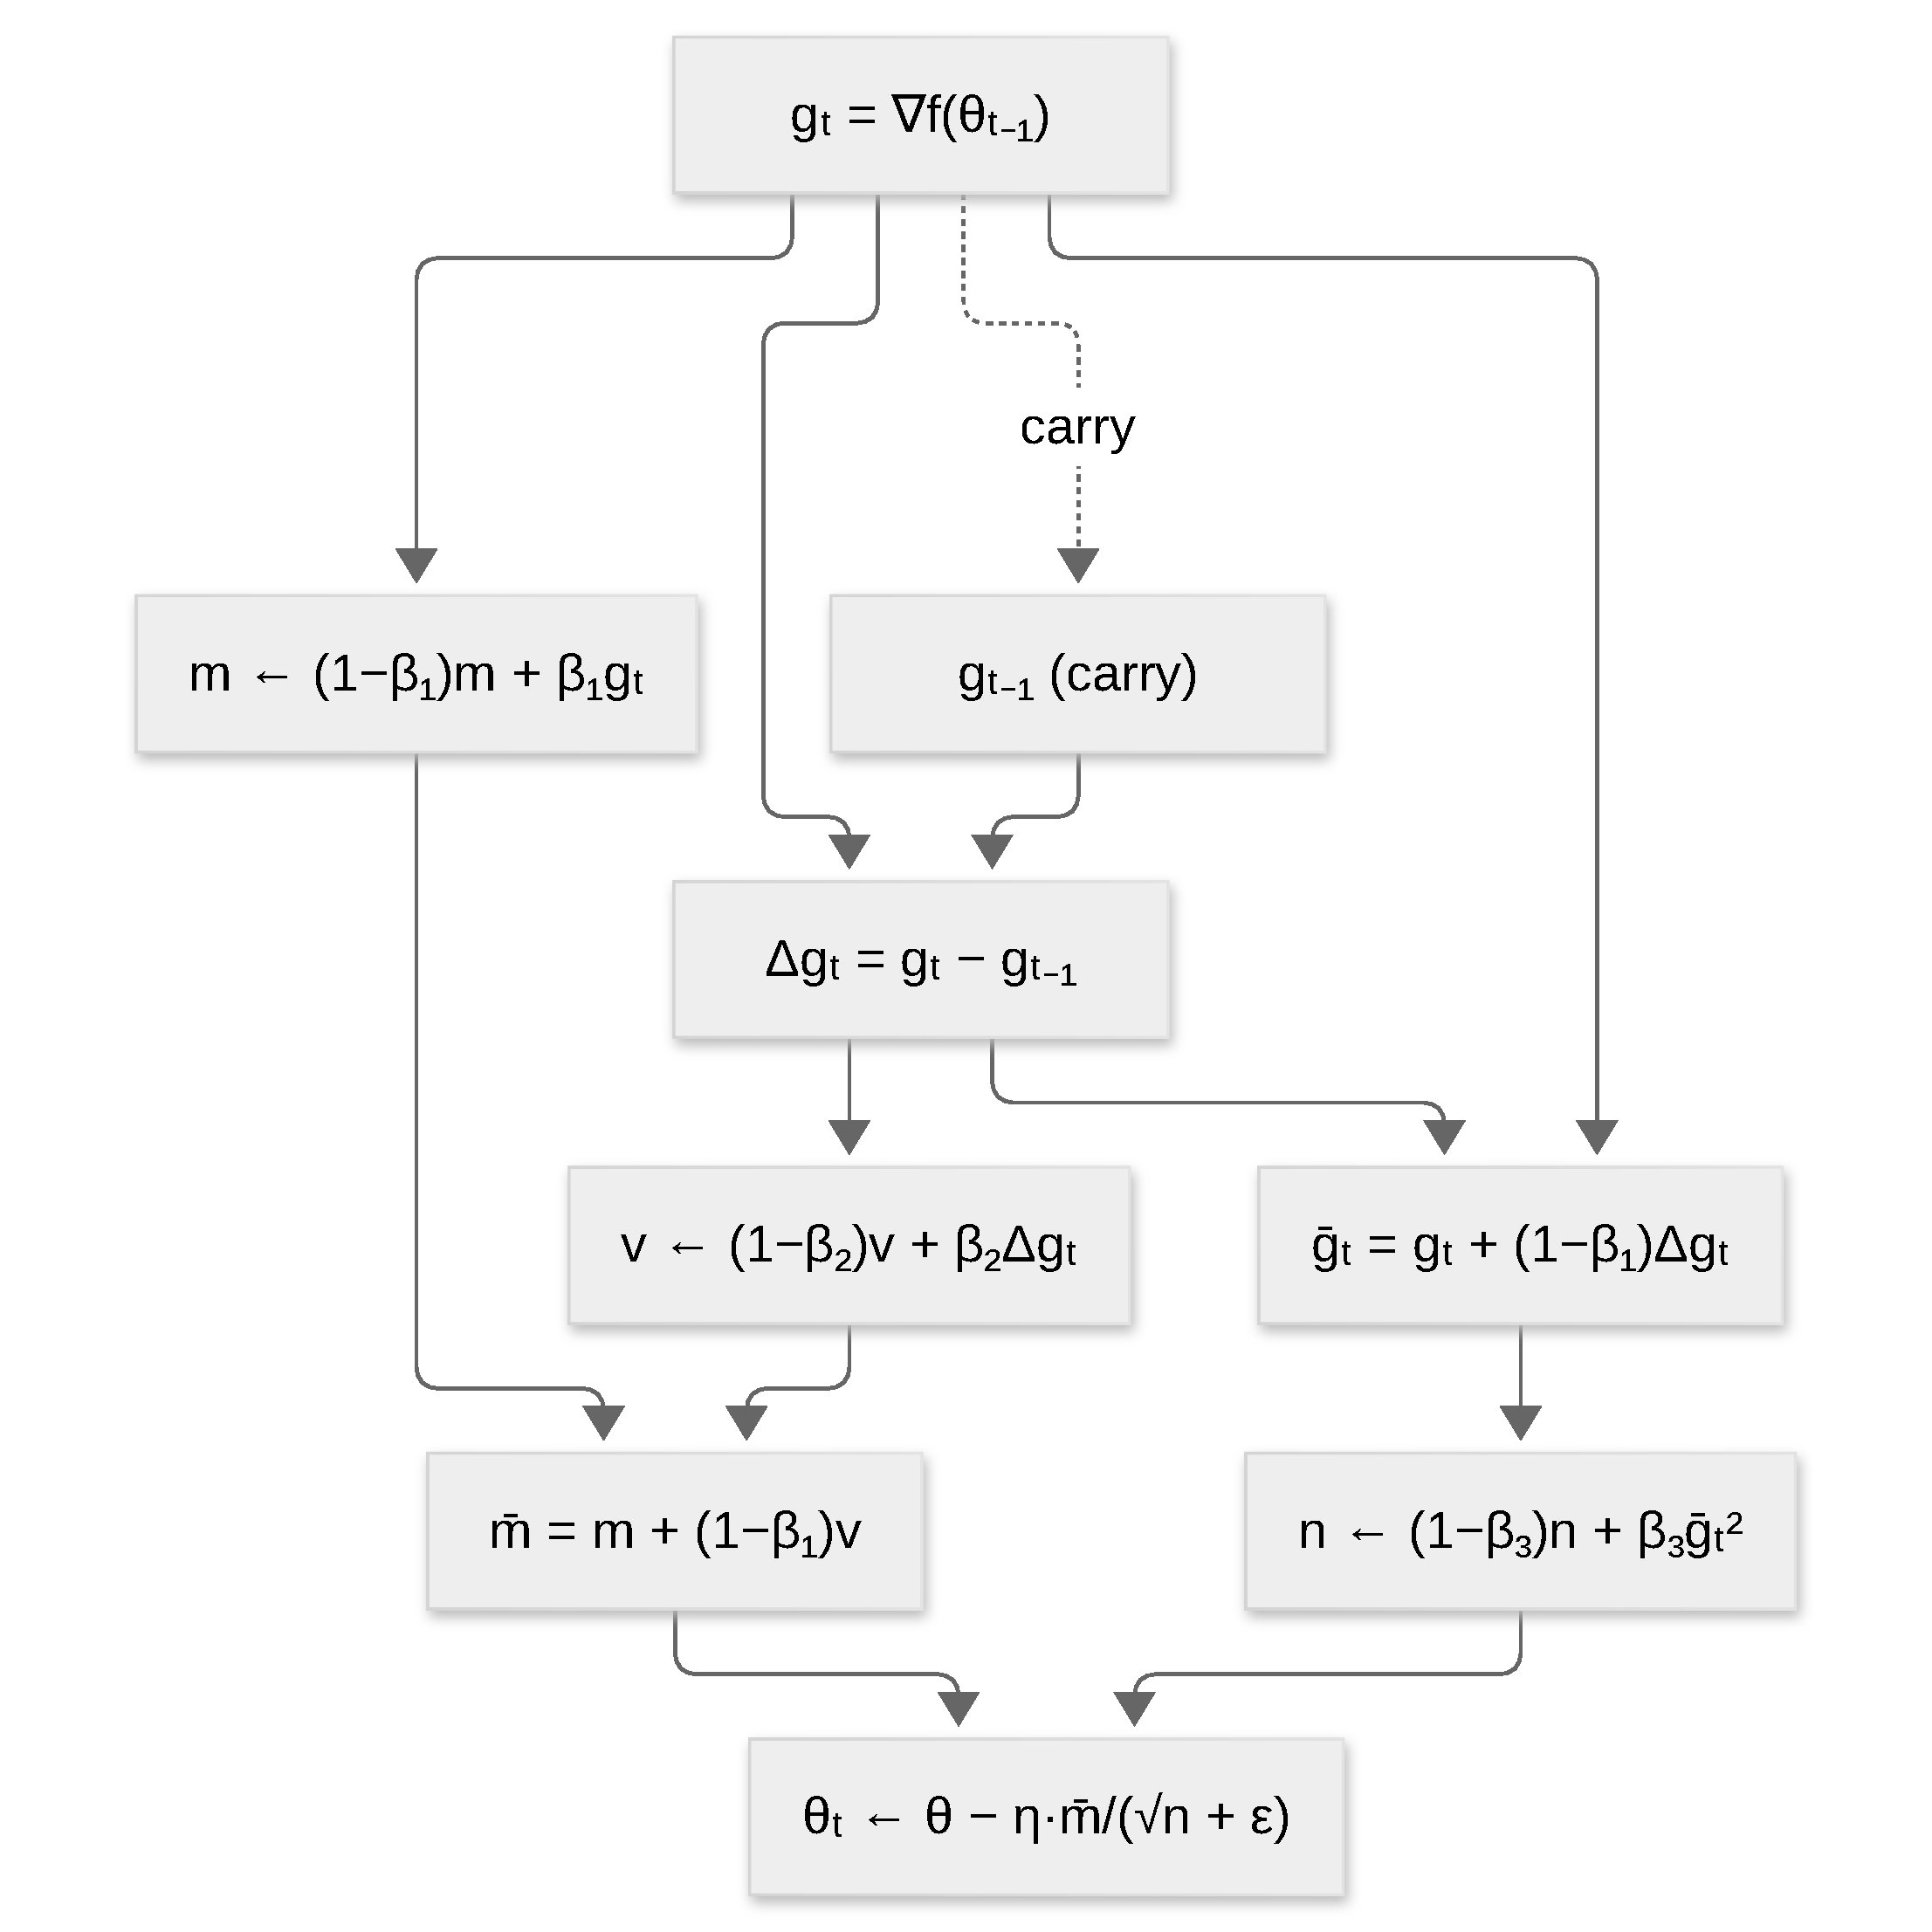
\includegraphics{figures/optimizers/adan.pdf}}
\caption{Step flow of Adan: Nesterov momentum estimation from the gradient difference, with three state buffers and a combined momentum step.}
\label{fig:opt-adan}
\end{figure}
Adan reformulates Nesterov acceleration without the extra gradient computation required by classical Nesterov SGD. The algorithm maintains three momentum buffers:
\begin{align}
m_t &= (1-\beta_1)m_{t-1} + \beta_1 g_t \quad\text{(first moment)} \\
v_t &= (1-\beta_2)v_{t-1} + \beta_2(g_t - g_{t-1}) \quad\text{(velocity/gradient difference)} \\
n_t &= (1-\beta_3)n_{t-1} + \beta_3[g_t + (1-\beta_1)(g_t-g_{t-1})]^2 \quad\text{(Nesterov second moment)}
\end{align}
The \textbf{Nesterov Momentum Estimation} (NME) term $\bar{g}_t = g_t + (1-\beta_1)(g_t-g_{t-1})$ estimates the gradient at a future position without evaluating it. The update combines momentum with velocity:
\[\bar{m}_t = m_t + (1-\beta_1)v_t, \quad \theta_{t+1} = \theta_t - \eta\frac{\bar{m}_t}{\sqrt{n_t}+\epsilon}\]

\begin{algorithm}[H]
\caption{Adan (Adaptive Nesterov Momentum)}
\label{alg:adan}
\begin{algorithmic}[1]
\Require Initial parameters $\theta_0$, learning rate $\eta$, $\beta_1, \beta_2, \beta_3 \in (0,1)$
\Ensure Updated parameters $\theta_T$
\State Initialize: $m \gets 0$, $v \gets 0$, $n \gets 0$, $g_{-1} \gets 0$ (previous gradient)
\For{$t = 1, 2, \ldots, T$}
    \State $g_t \gets \nabla f(\theta_{t-1})$
    \State $m \gets (1-\beta_1) m + \beta_1 g_t$
    \State $\Delta g_t \gets g_t - g_{t-1}$
    \State $v \gets (1-\beta_2) v + \beta_2 \Delta g_t$
    \State Nesterov estimation: $\bar{g}_t \gets g_t + (1-\beta_1) \Delta g_t$
    \State $n \gets (1-\beta_3) n + \beta_3 \bar{g}_t^2$
    \State Combined momentum: $\bar{m} \gets m + (1-\beta_1) v$
    \State $\theta_t \gets \theta_{t-1} - \eta (\bar{m} / (\sqrt{n} + \epsilon))$
    \State $g_{t-1} \gets g_t$
\EndFor
\Return $\theta_T$
\end{algorithmic}
\end{algorithm}

\paragraph{Cons.}
\begin{itemize}[leftmargin=*]
\item Three momentum-like buffers increase memory overhead relative to Adam.
\item Additional gradient-difference bookkeeping per step.
\end{itemize}

\paragraph{Pros.}
\begin{itemize}[leftmargin=*]
\item Nesterov-style acceleration without an extra gradient evaluation.
\item Fast convergence across diverse architectures (CNNs, GANs, transformers).
\end{itemize}

\paragraph{ADOPT (Adam with Optimal Pruned Tuning).}
\begin{figure}[H]
\centering
\fitfigure{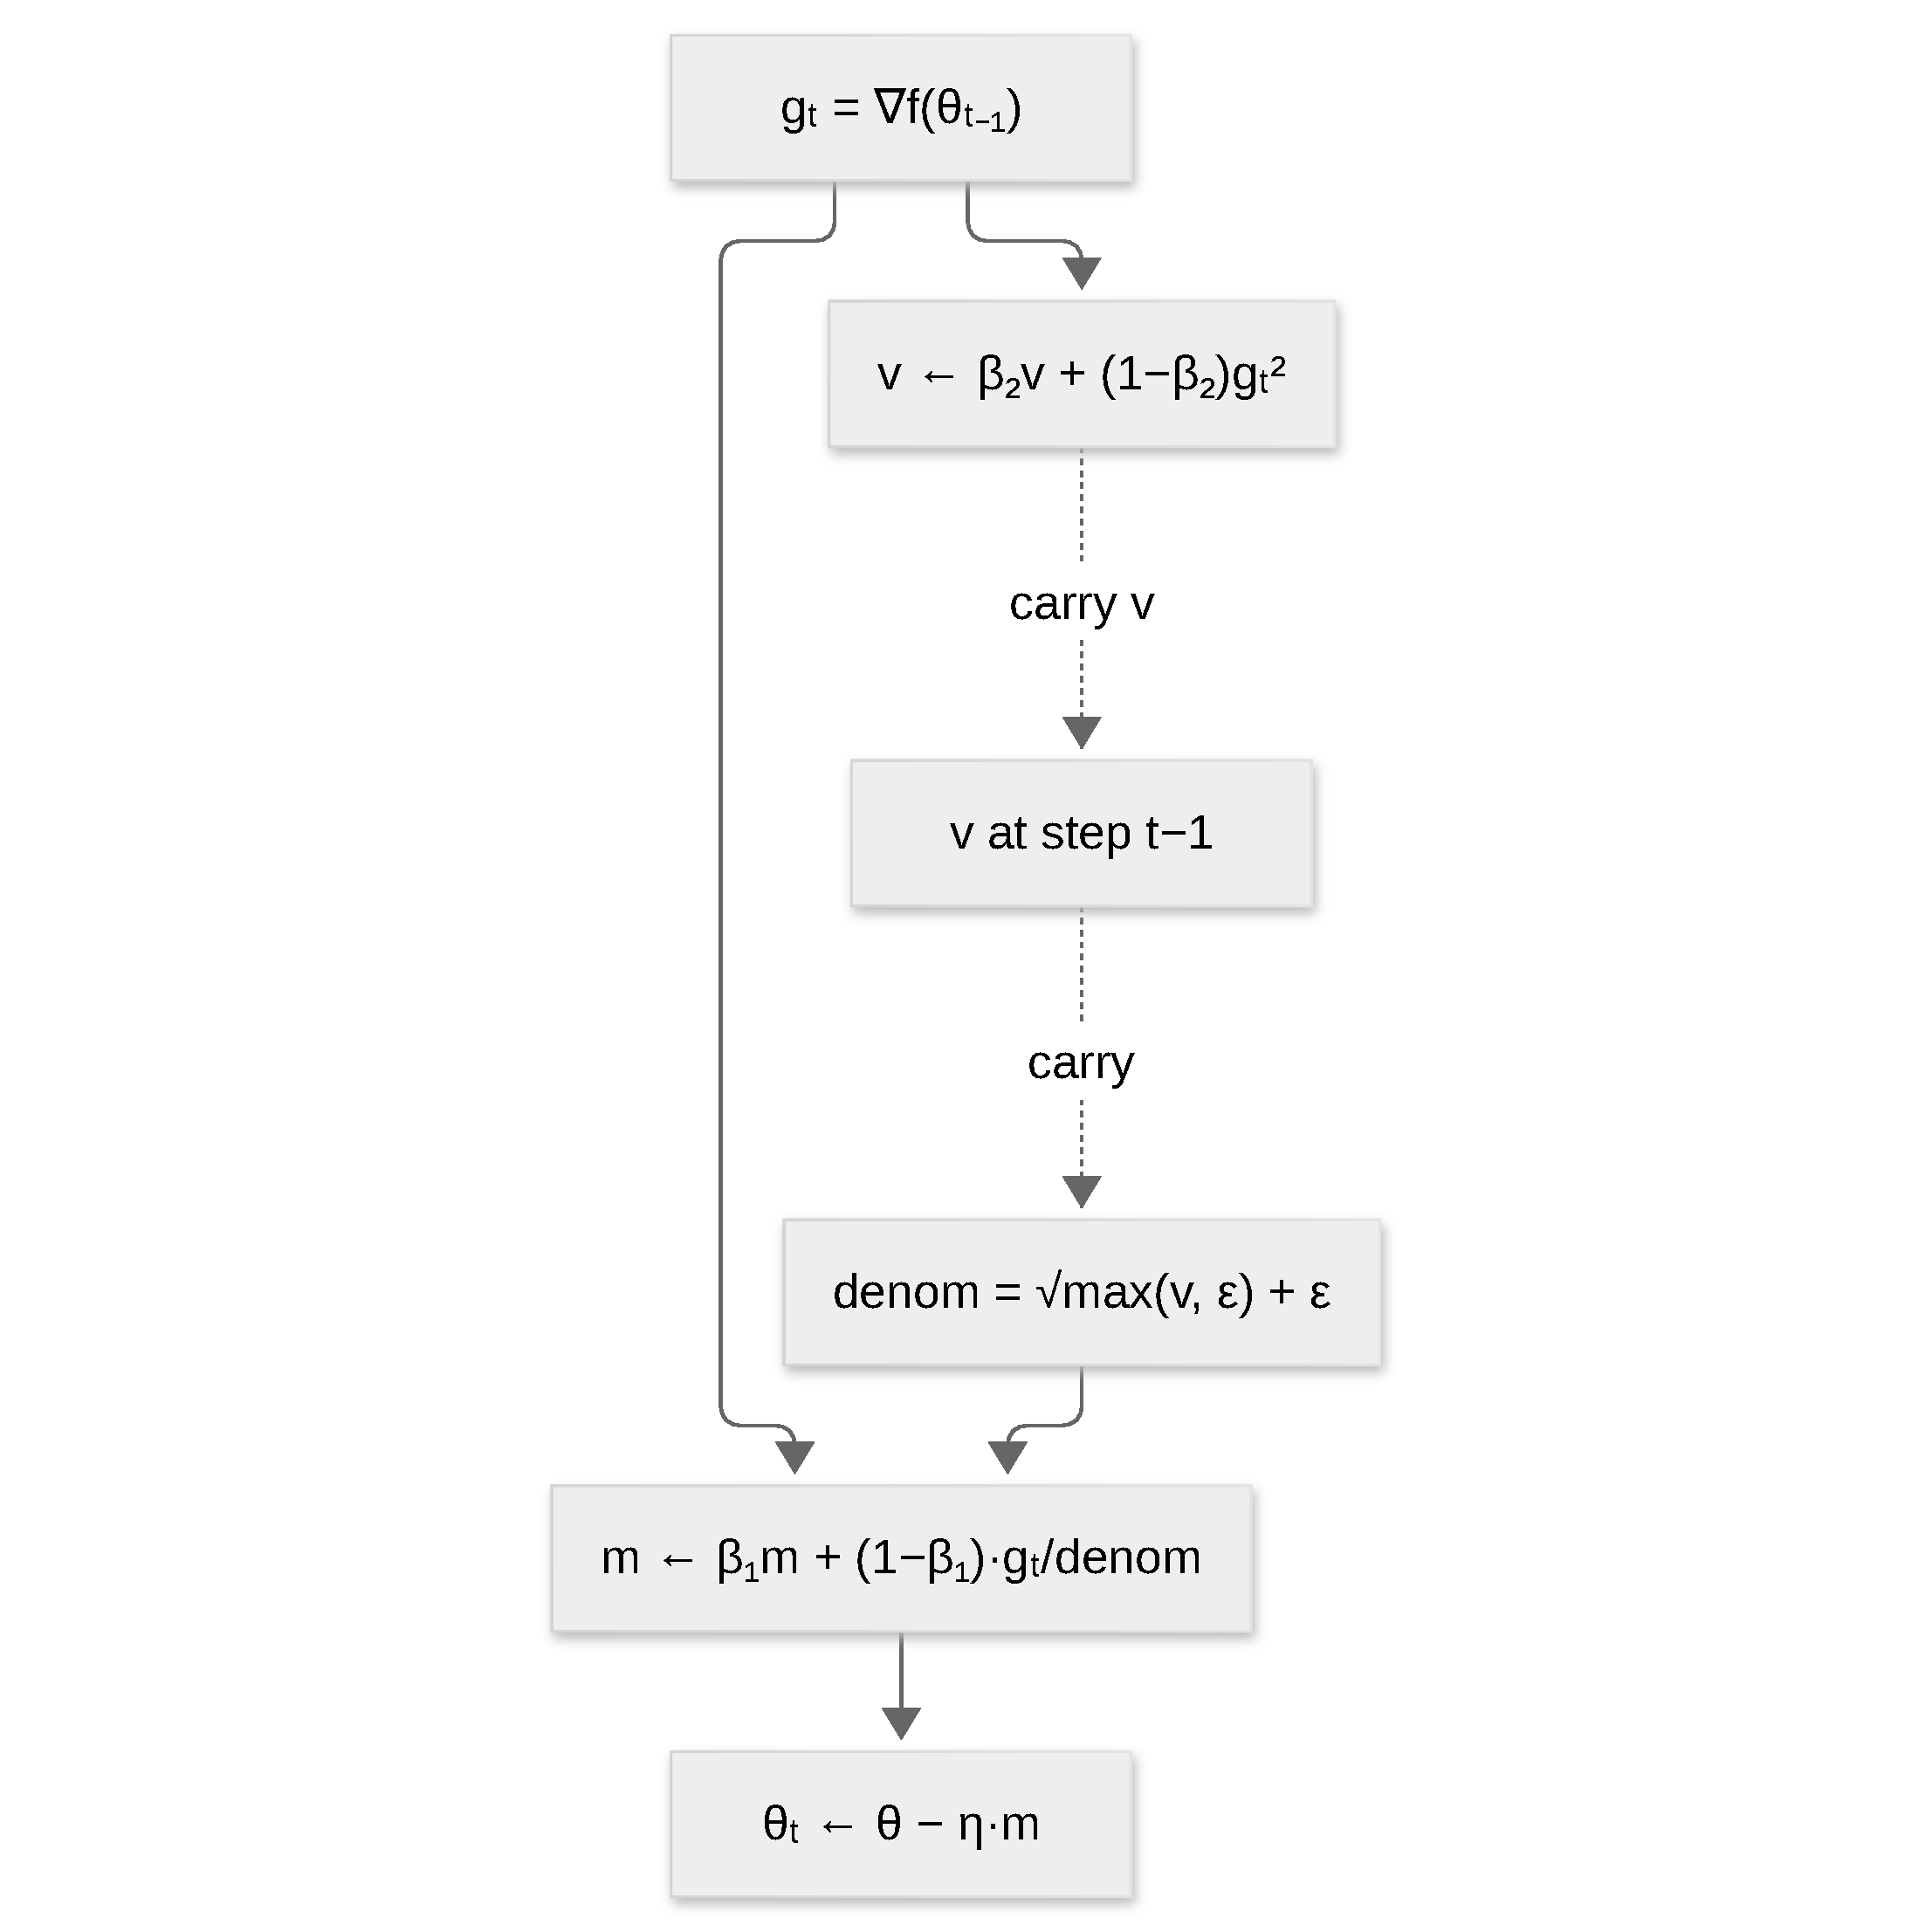
\includegraphics{figures/optimizers/adopt.pdf}}
\caption{Step flow of ADOPT: the second moment from the previous step normalizes the current gradient before the first-moment update.}
\label{fig:opt-adopt}
\end{figure}
ADOPT fixes a fundamental theoretical issue in Adam: the gradient appears in both the first moment and second moment estimates, creating circularity. ADOPT \textbf{decouples} by using the previous step's second moment for the denominator:
\begin{align}
v_t &= \beta_2 v_{t-1} + (1-\beta_2)g_t^2 \\
m_t &= \beta_1 m_{t-1} + (1-\beta_1)\frac{g_t}{\sqrt{v_{t-1}}+\epsilon} \quad\text{(uses $v_{t-1}$, not $v_t$)} \\
\theta_{t+1} &= \theta_t - \eta m_t
\end{align}

\begin{algorithm}[H]
\caption{ADOPT (Adam with Optimal Pruned Tuning)}
\label{alg:adopt}
\begin{algorithmic}[1]
\Require Initial parameters $\theta_0$, learning rate $\eta$, $\beta_1, \beta_2$, tolerance $\epsilon$
\Ensure Updated parameters $\theta_T$
\State Initialize: $m \gets 0$, $v \gets 0$
\For{$t = 1, 2, \ldots, T$}
    \State $g_t \gets \nabla f(\theta_{t-1})$
    \If{weight\_decay $> 0$}
        \State $\theta_{t-1} \gets \theta_{t-1}(1 - \eta\lambda)$
    \EndIf
    \State Use \textbf{previous} second moment: $\text{denom} \gets \sqrt{\max(v, \epsilon)} + \epsilon$
    \State Update first moment using previous variance: $m \gets \beta_1 m + (1-\beta_1)(g_t / \text{denom})$
    \State Update second moment with \textbf{current} gradient: $v \gets \beta_2 v + (1-\beta_2) g_t^2$
    \State $\theta_t \gets \theta_{t-1} - \eta m$
\EndFor
\Return $\theta_T$
\end{algorithmic}
\end{algorithm}

\paragraph{Cons.}
\begin{itemize}[leftmargin=*]
\item Requires keeping the previous second moment as an explicit denominator.
\item Empirical gains are architecture- and tuning-dependent.
\end{itemize}

\paragraph{Pros.}
\begin{itemize}[leftmargin=*]
\item Removes Adam's gradient circularity and attains the optimal convergence rate $O(1/\sqrt{T})$ with \textbf{any} $\beta_2 \in (0,1)$, without bounded-noise assumptions.
\item Drop-in Adam replacement with comparable or superior empirical performance across vision, NLP, RL, and generative modeling.
\end{itemize}

\paragraph{AdEMAMix (Exponential Moving Average Mixture).}
\begin{figure}[H]
\centering
\fitfigure{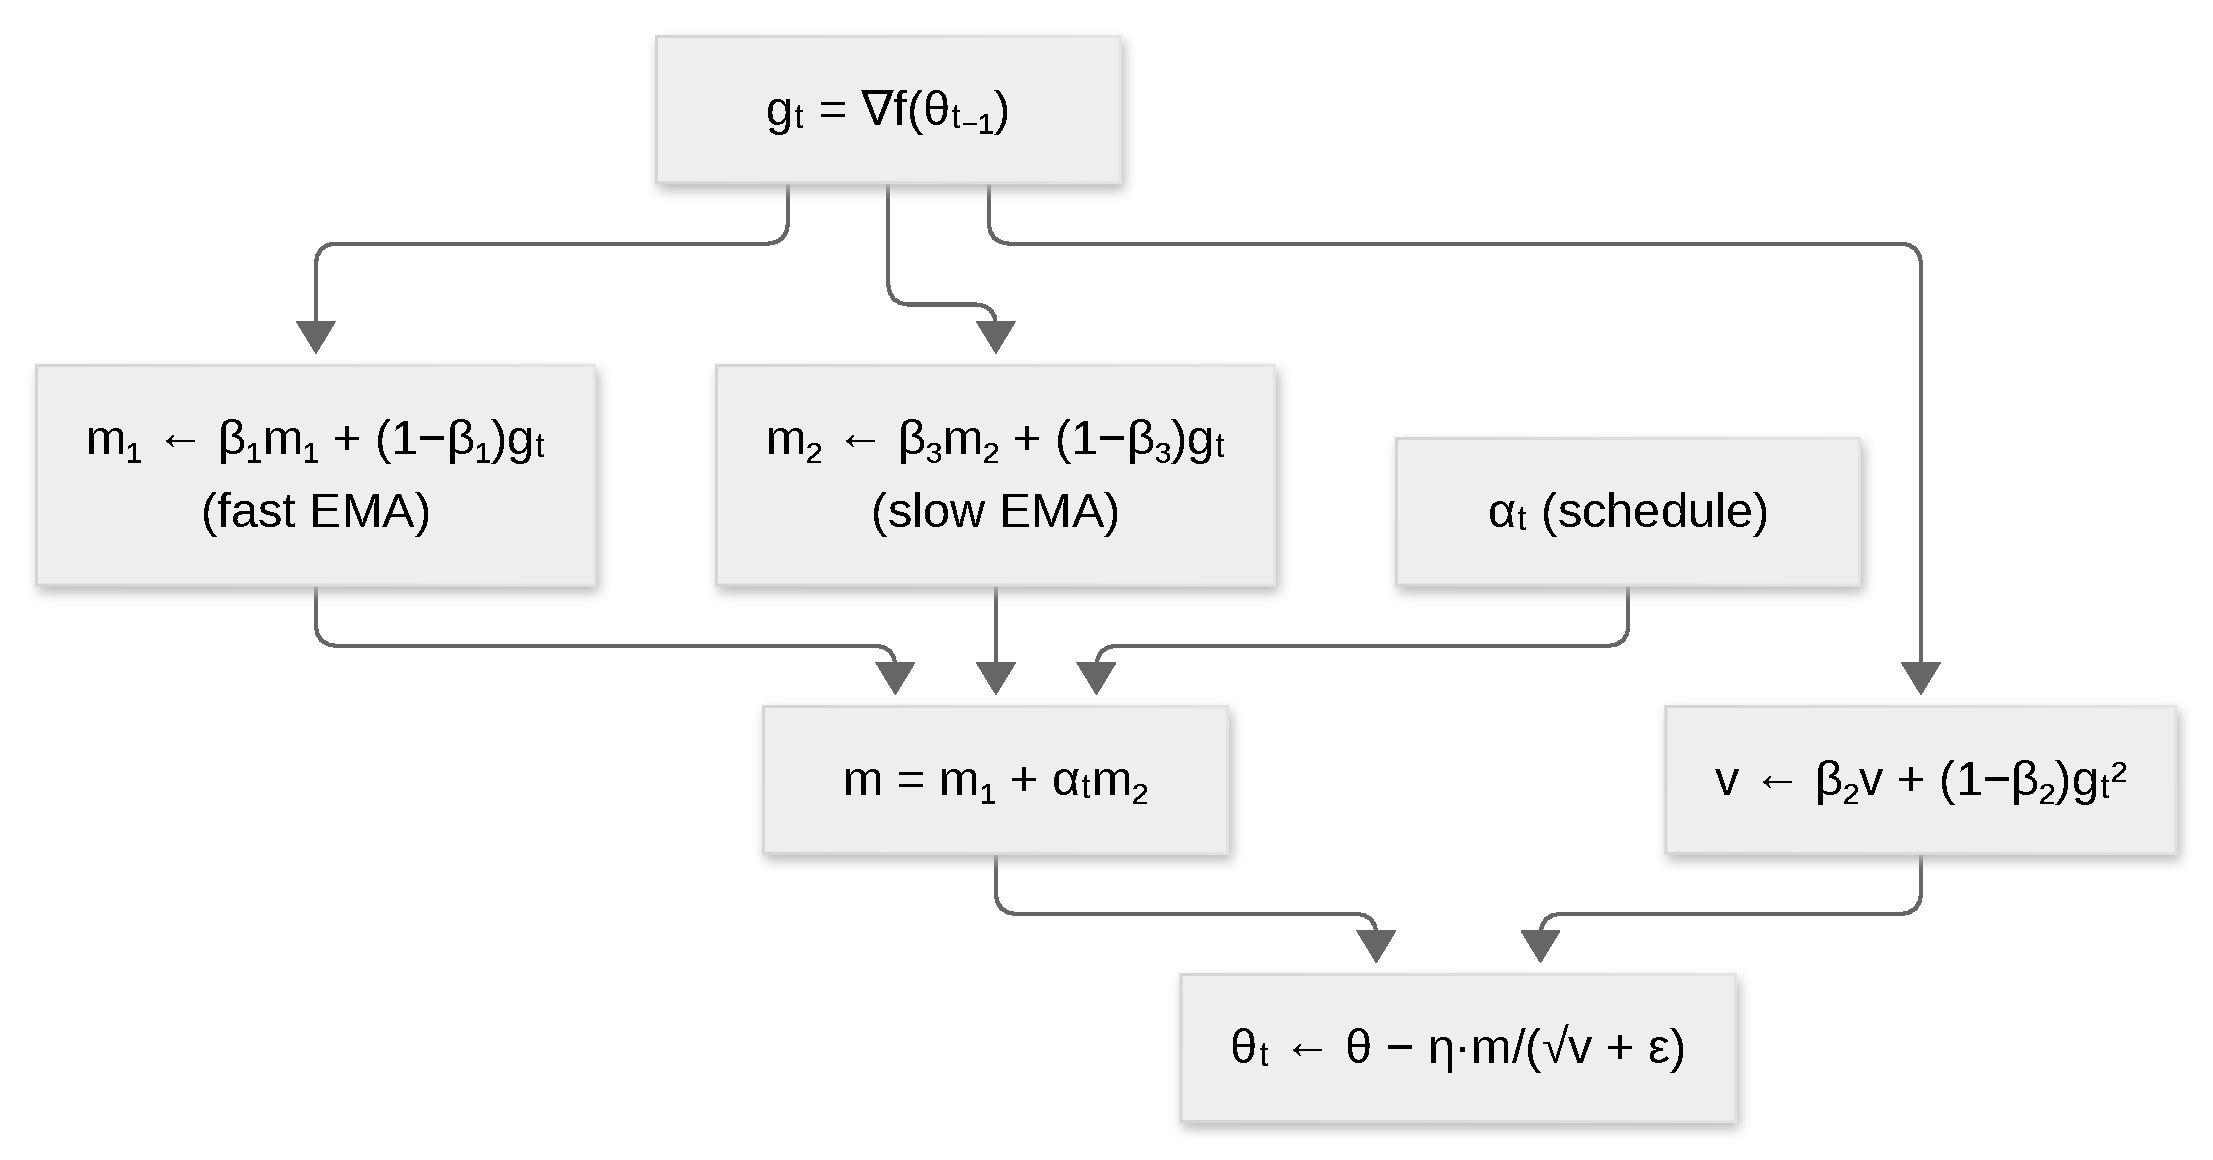
\includegraphics{figures/optimizers/ademamix.pdf}}
\caption{Step flow of AdEMAMix: parallel fast and slow gradient EMAs, mixed with a scheduled weight $\alpha_t$ before the adaptive update.}
\label{fig:opt-ademamix}
\end{figure}
AdEMAMix replaces Adam's single EMA of gradients with a \textbf{mixture of two EMAs}: one fast-decaying and one slow-decaying. This addresses the observation that gradients remain informative over tens of thousands of steps, not just hundreds:
\begin{align}
m_{1,t} &= \beta_1 m_{1,t-1} + (1-\beta_1)g_t \quad\text{(fast EMA, $\beta_1 \approx 0.9$)} \\
m_{2,t} &= \beta_3 m_{2,t-1} + (1-\beta_3)g_t \quad\text{(slow EMA, $\beta_3 \approx 0.9999$)} \\
v_t &= \beta_2 v_{t-1} + (1-\beta_2)g_t^2 \\
m_t &= m_{1,t} + \alpha_t m_{2,t} \quad\text{(mixture with scheduled weight $\alpha_t$)} \\
\theta_{t+1} &= \theta_t - \eta\frac{m_t}{\sqrt{v_t}+\epsilon}
\end{align}
The mixture weight $\alpha_t$ typically increases during training, allowing the fast EMA to provide immediate adaptation while the slow EMA accumulates long-range gradient correlations.

\begin{algorithm}[H]
\caption{AdEMAMix (Exponential Moving Average Mixture)}
\label{alg:ademamix}
\begin{algorithmic}[1]
\Require Initial parameters $\theta_0$, learning rate $\eta$, $\beta_1$ (fast), $\beta_3$ (slow), $\beta_2$ (second moment)
\Require Mixture weight $\alpha_t$ (typically increasing), tolerance $\epsilon$
\Ensure Updated parameters $\theta_T$
\State Initialize: $m_1 \gets 0$ (fast EMA), $m_2 \gets 0$ (slow EMA), $v \gets 0$
\For{$t = 1, 2, \ldots, T$}
    \State $g_t \gets \nabla f(\theta_{t-1})$
    \If{weight\_decay $> 0$}
        \State $\theta_{t-1} \gets \theta_{t-1}(1 - \eta\lambda)$
    \EndIf
    \State $m_1 \gets \beta_1 m_1 + (1-\beta_1) g_t$ \Comment{Fast EMA}
    \State $m_2 \gets \beta_3 m_2 + (1-\beta_3) g_t$ \Comment{Slow EMA}
    \State $v \gets \beta_2 v + (1-\beta_2) g_t^2$
    \State $m_t \gets m_1 + \alpha_t m_2$ \Comment{Mixture}
    \State $\theta_t \gets \theta_{t-1} - \eta (m_t / (\sqrt{v} + \epsilon))$
\EndFor
\Return $\theta_T$
\end{algorithmic}
\end{algorithm}

\paragraph{Cons.}
\begin{itemize}[leftmargin=*]
\item Two gradient EMAs plus the second moment roughly triple Adam's optimizer state.
\item The mixture schedule $\alpha_t$ adds a hyperparameter to tune.
\end{itemize}

\paragraph{Pros.}
\begin{itemize}[leftmargin=*]
\item Exploits gradient information that remains informative over tens of thousands of steps.
\item A 1.3B model on 101B tokens matches AdamW on 197B tokens (95\% data-efficiency gain), suggesting reduced forgetting.
\end{itemize}

\paragraph{MARS (Make Adaptive learning Rates Shine).}
\begin{figure}[H]
\centering
\fitfigure{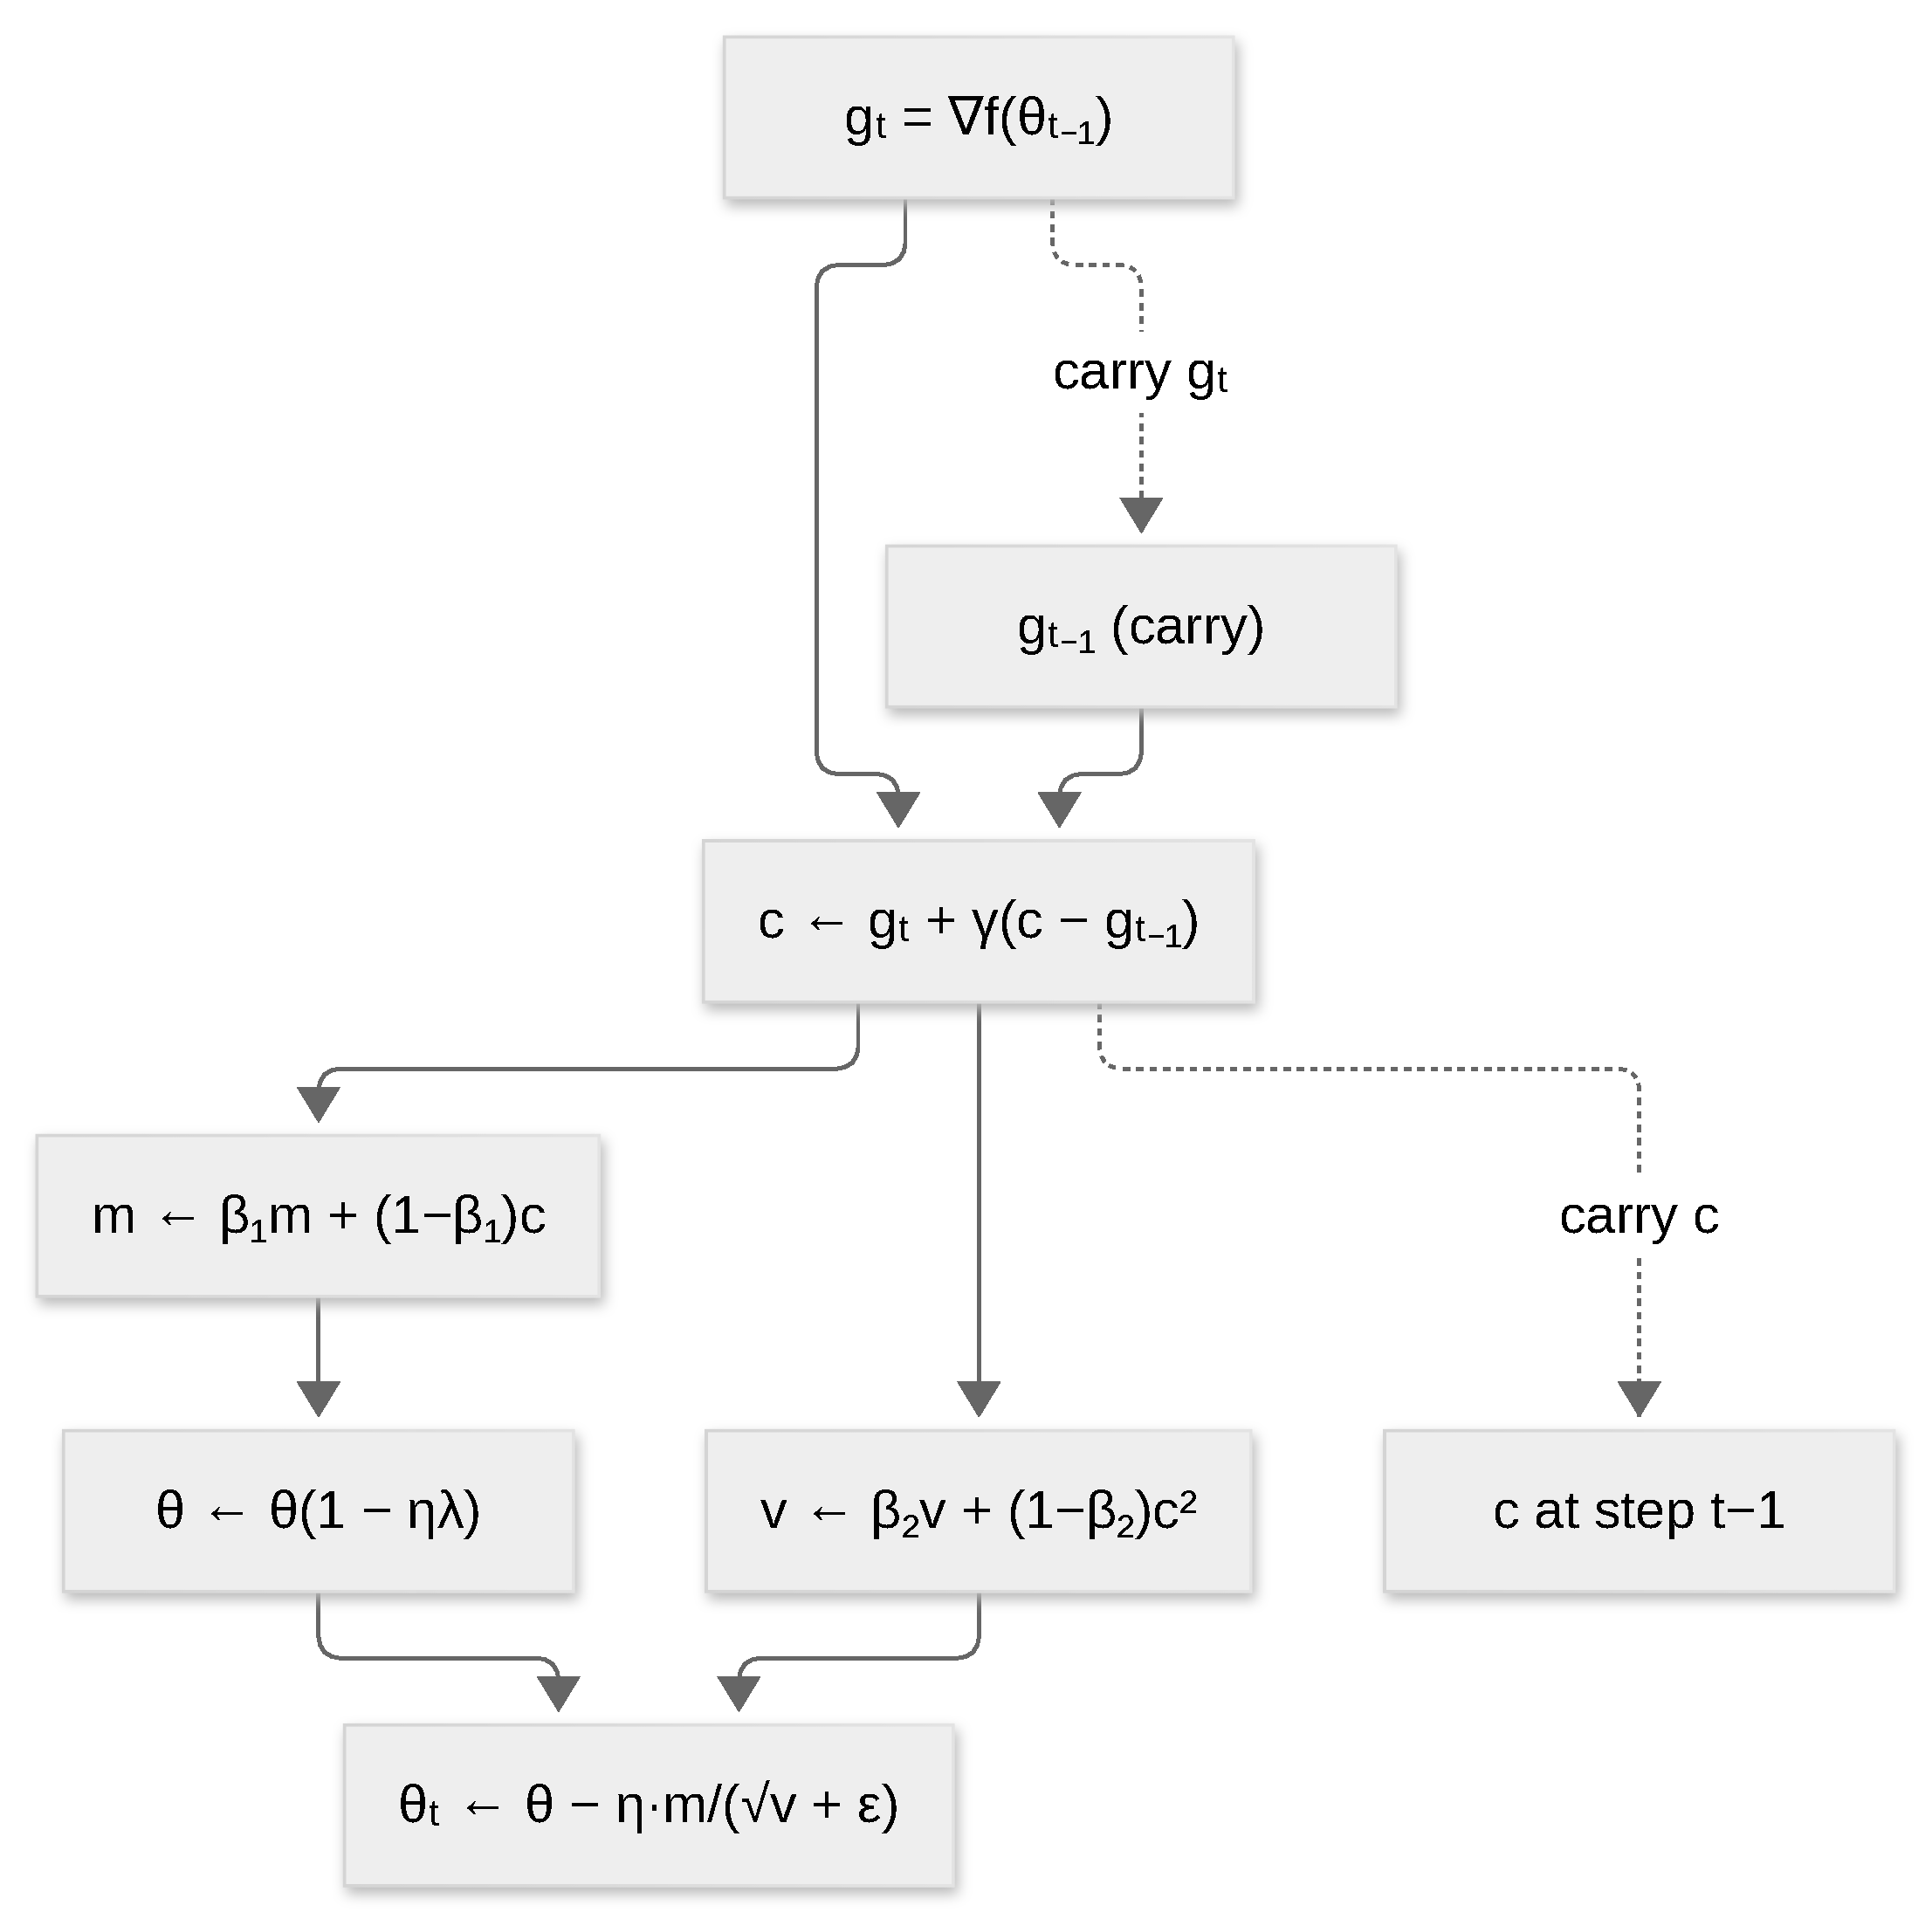
\includegraphics{figures/optimizers/mars.pdf}}
\caption{Step flow of MARS: a recursive variance-reduced gradient estimate feeding Adam-style first and second moments.}
\label{fig:opt-mars}
\end{figure}
MARS combines preconditioned gradient methods (e.g., AdamW) with \textbf{variance reduction} via scaled stochastic recursive momentum. The core innovation is a variance-reduced gradient estimate:
\begin{align}
c_t &= g_t + \gamma(c_{t-1} - g_{t-1}) \quad\text{(SVRG-style recursive estimate)} \\
m_t &= \beta_1 m_{t-1} + (1-\beta_1)c_t \\
v_t &= \beta_2 v_{t-1} + (1-\beta_2)c_t^2 \\
\theta_{t+1} &= \theta_t - \eta\frac{m_t}{\sqrt{v_t}+\epsilon}
\end{align}
where $\gamma \in [0.01, 0.1]$ controls how much historical gradient information is retained. The variance-reduced gradient $c_t$ acts as an implicit noise filter, amplifying consistent signal directions and dampening contradictory noise.

\begin{algorithm}[H]
\caption{MARS (Make Adaptive learning Rates Shine)}
\label{alg:mars}
\begin{algorithmic}[1]
\Require Initial parameters $\theta_0$, learning rate $\eta$, $\beta_1, \beta_2$, weight decay $\lambda$
\Require Variance reduction coefficient $\gamma \in [0.01, 0.1]$
\Ensure Updated parameters $\theta_T$
\State Initialize: $m \gets 0$, $v \gets 0$, $c \gets 0$ (variance-reduced gradient), $g_{-1} \gets 0$
\For{$t = 1, 2, \ldots, T$}
    \State $g_t \gets \nabla f(\theta_{t-1})$
    \State Variance reduction: $c \gets g_t + \gamma(c - g_{t-1})$
    \State $m \gets \beta_1 m + (1-\beta_1) c$
    \State $v \gets \beta_2 v + (1-\beta_2) c^2$
    \If{weight\_decay $> 0$}
        \State $\theta_{t-1} \gets \theta_{t-1}(1 - \eta\lambda)$
    \EndIf
    \State $\theta_t \gets \theta_{t-1} - \eta (m / (\sqrt{v} + \epsilon))$
    \State $g_{t-1} \gets g_t$
\EndFor
\Return $\theta_T$
\end{algorithmic}
\end{algorithm}

\paragraph{Cons.}
\begin{itemize}[leftmargin=*]
\item Stores the variance-reduced gradient and the previous gradient in addition to Adam's moments.
\item The variance-reduction coefficient $\gamma \in [0.01, 0.1]$ must be tuned.
\end{itemize}

\paragraph{Pros.}
\begin{itemize}[leftmargin=*]
\item Acts as an implicit noise filter, amplifying consistent directions and dampening contradictory noise.
\item MARS-AdamW consistently outperforms bare AdamW by significant margins on GPT-2 pretraining.
\end{itemize}

\paragraph{Cautious Optimizers (Cautious AdamW, Cautious Lion).}
\begin{figure}[H]
\centering
\fitfigure{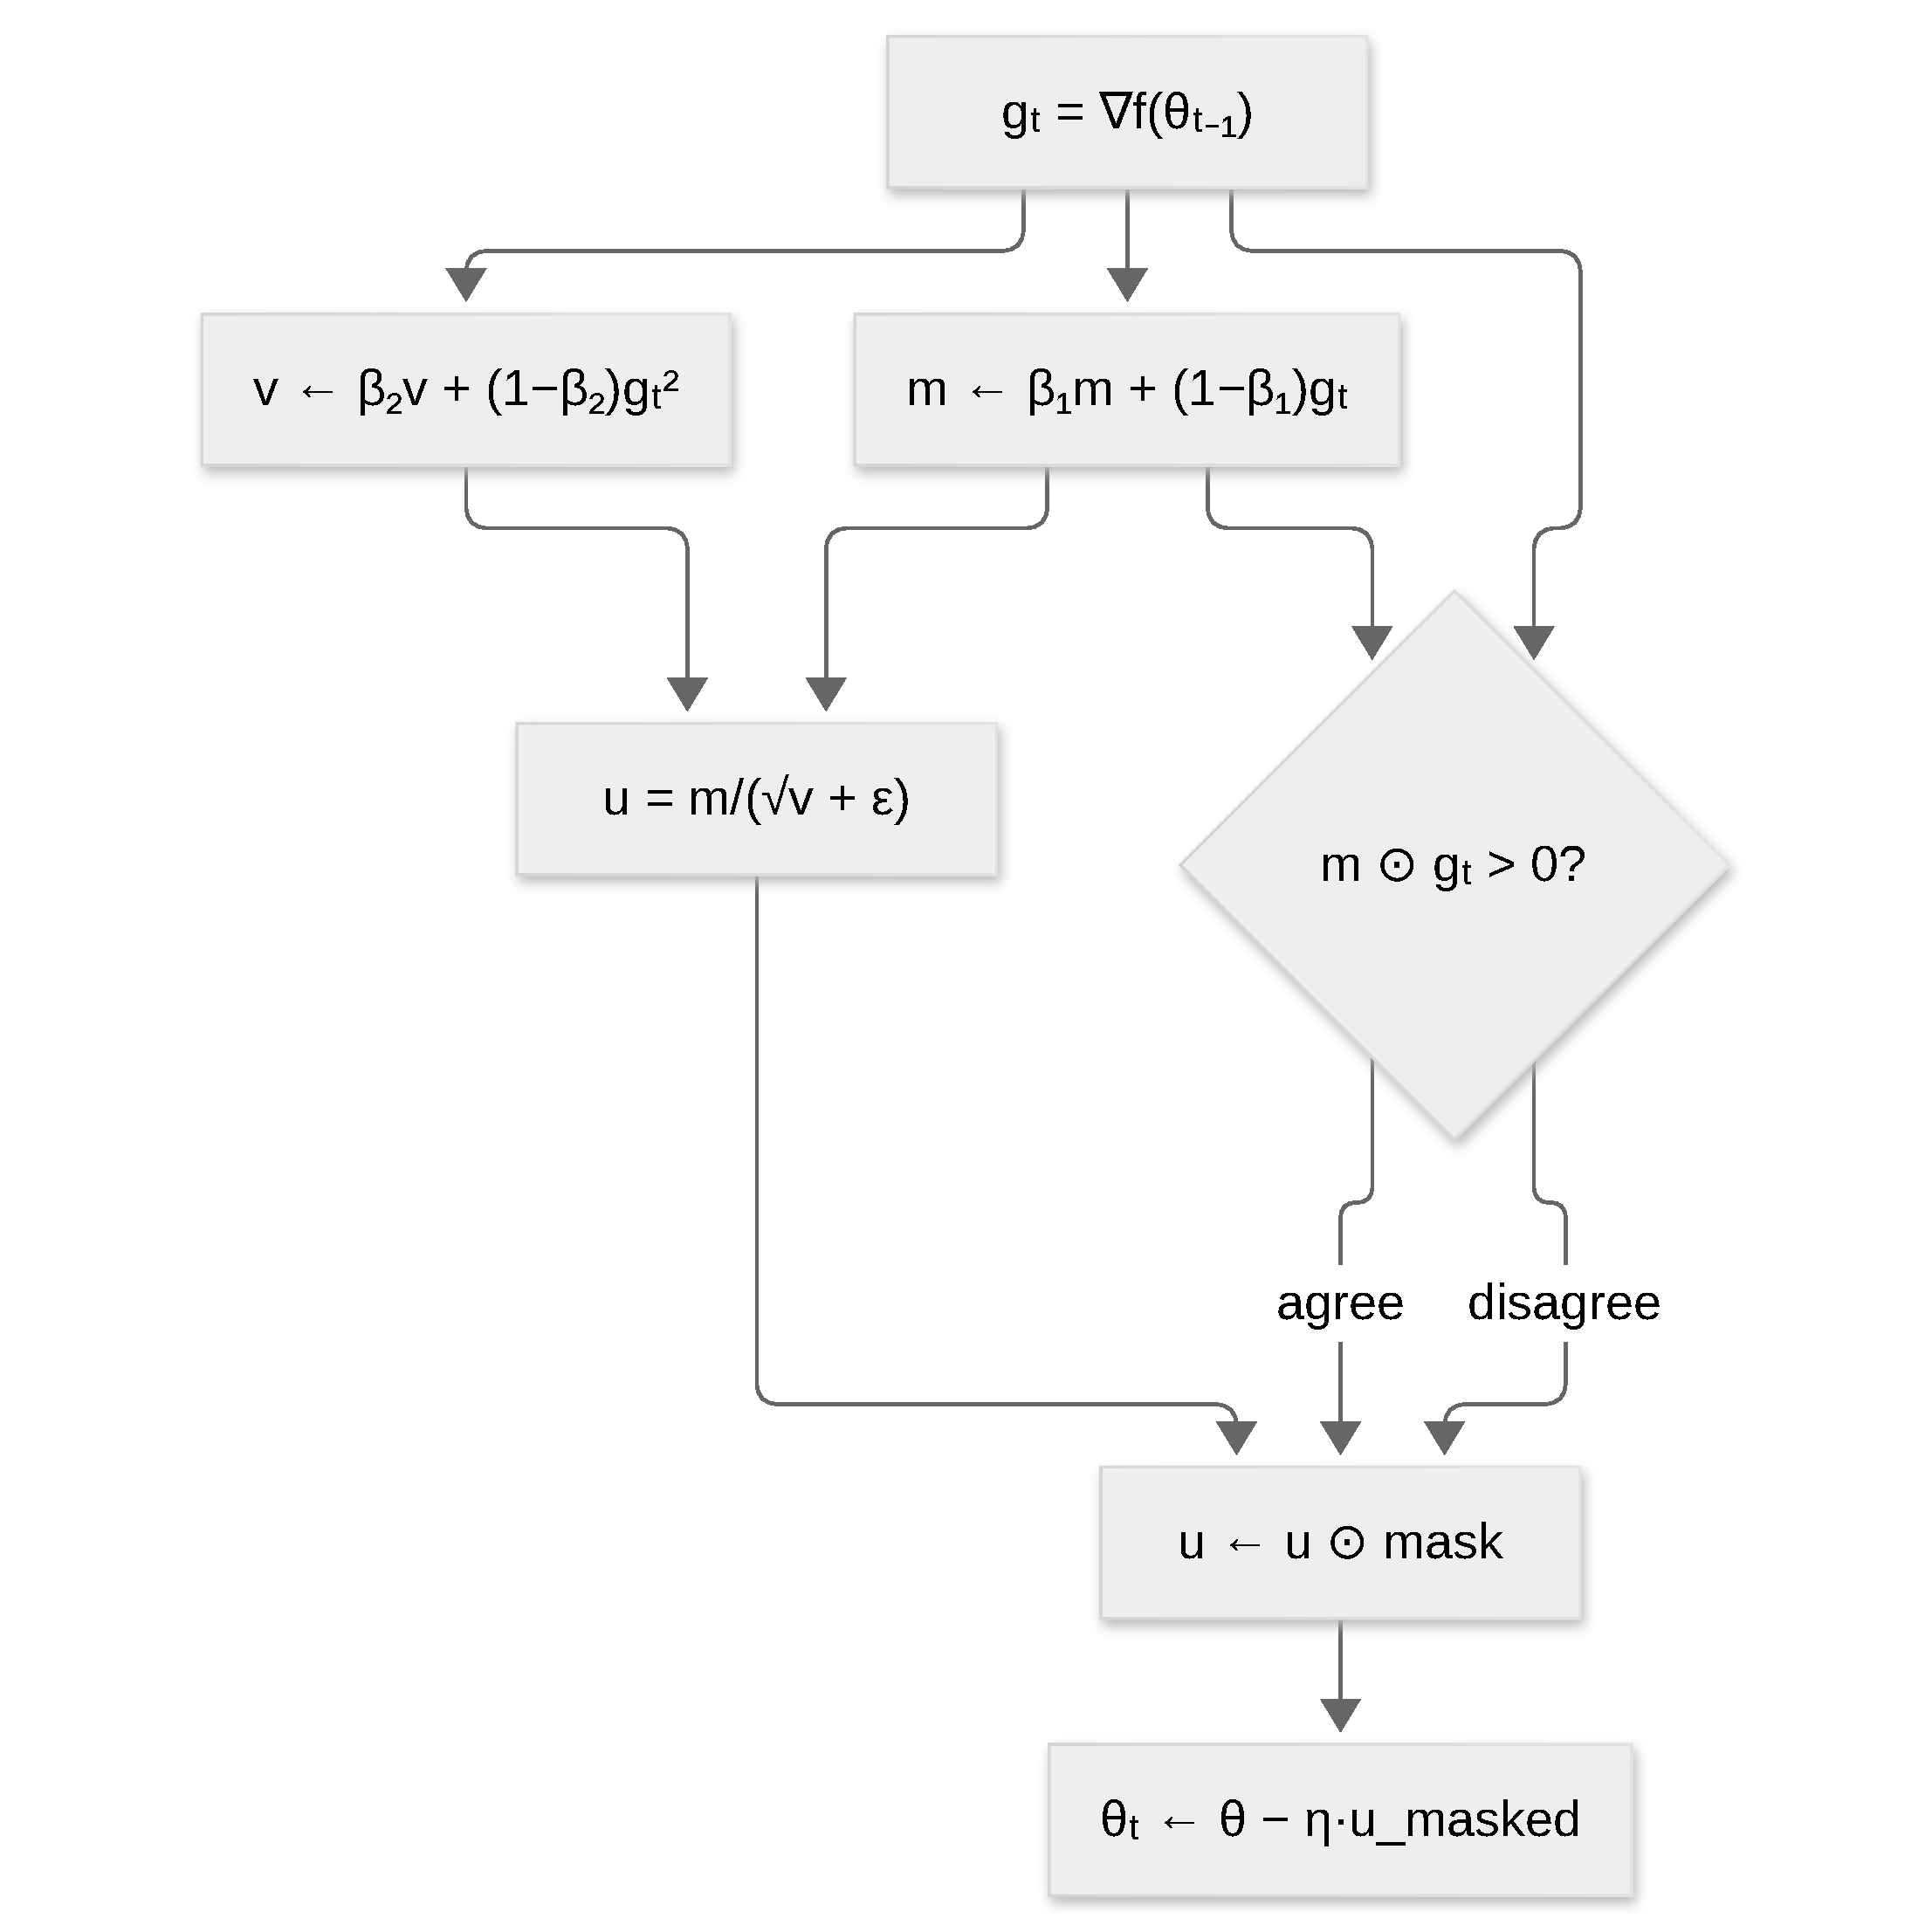
\includegraphics{figures/optimizers/cautious.pdf}}
\caption{Step flow of Cautious AdamW: a consensus mask keeps only update coordinates where momentum and gradient agree.}
\label{fig:opt-cautious}
\end{figure}
The Cautious framework applies a \textbf{one-line modification} to any momentum-based optimizer: mask the update so that only dimensions where momentum and gradient directions agree are applied:
\begin{align}
\text{mask}_i &= \begin{cases} 1 & \text{if } m_t[i] \cdot g_t[i] > 0 \quad\text{(agreement)} \\ 0 & \text{otherwise} \end{cases} \\
u_t &= \left(\frac{m_t}{\sqrt{v_t}+\epsilon}\right) \odot \text{mask} \quad\text{(element-wise masking)} \\
\theta_{t+1} &= \theta_t - \eta u_t
\end{align}
The intuition: momentum $m_t$ estimates the gradient direction from history; the current gradient $g_t$ is instantaneous signal. When both agree, the optimizer is confident and should update aggressively. When they disagree, the optimizer is conflicted---the historical trend points toward a region that may have been good before, but current evidence contradicts it. By masking conflicted dimensions, Cautious becomes more conservative and avoids corrupted steps.

\begin{algorithm}[H]
\caption{Cautious AdamW (Consensus-based Update Masking)}
\label{alg:cautious}
\begin{algorithmic}[1]
\Require Initial parameters $\theta_0$, learning rate $\eta$, $\beta_1, \beta_2$, weight decay $\lambda$
\Ensure Updated parameters $\theta_T$
\State Initialize: $m \gets 0$, $v \gets 0$
\For{$t = 1, 2, \ldots, T$}
    \State $g_t \gets \nabla f(\theta_{t-1})$
    \State $m \gets \beta_1 m + (1-\beta_1) g_t$
    \State $v \gets \beta_2 v + (1-\beta_2) g_t^2$
    \State Consensus mask: $\text{mask}_i \gets 1$ if $m[i] \cdot g_t[i] > 0$, else $0$ \Comment{Agreement}
    \State Base Adam update: $u \gets m / (\sqrt{v} + \epsilon)$
    \State Apply mask: $u_{\text{masked}} \gets u \odot \text{mask}$ \Comment{Element-wise}
    \If{weight\_decay $> 0$}
        \State $\theta_{t-1} \gets \theta_{t-1}(1 - \eta\lambda)$
    \EndIf
    \State $\theta_t \gets \theta_{t-1} - \eta u_{\text{masked}}$
\EndFor
\Return $\theta_T$
\end{algorithmic}
\end{algorithm}

\paragraph{Cons.}
\begin{itemize}[leftmargin=*]
\item Masking can discard useful updates when momentum and gradient temporarily disagree.
\item Requires a base momentum optimizer plus the element-wise mask.
\end{itemize}

\paragraph{Pros.}
\begin{itemize}[leftmargin=*]
\item A one-line modification applicable to any momentum-based optimizer.
\item Up to \textbf{1.47$\times$ speedup} on Llama and MAE pretraining while preserving convergence guarantees.
\end{itemize}


\subsection{Large-Batch, Memory-Efficient, and Parameter-Free Optimizers}
\paragraph{LAMB (Layer-wise Adaptive Moments optimizer for Batch training).}
\begin{figure}[H]
\centering
\fitfigure{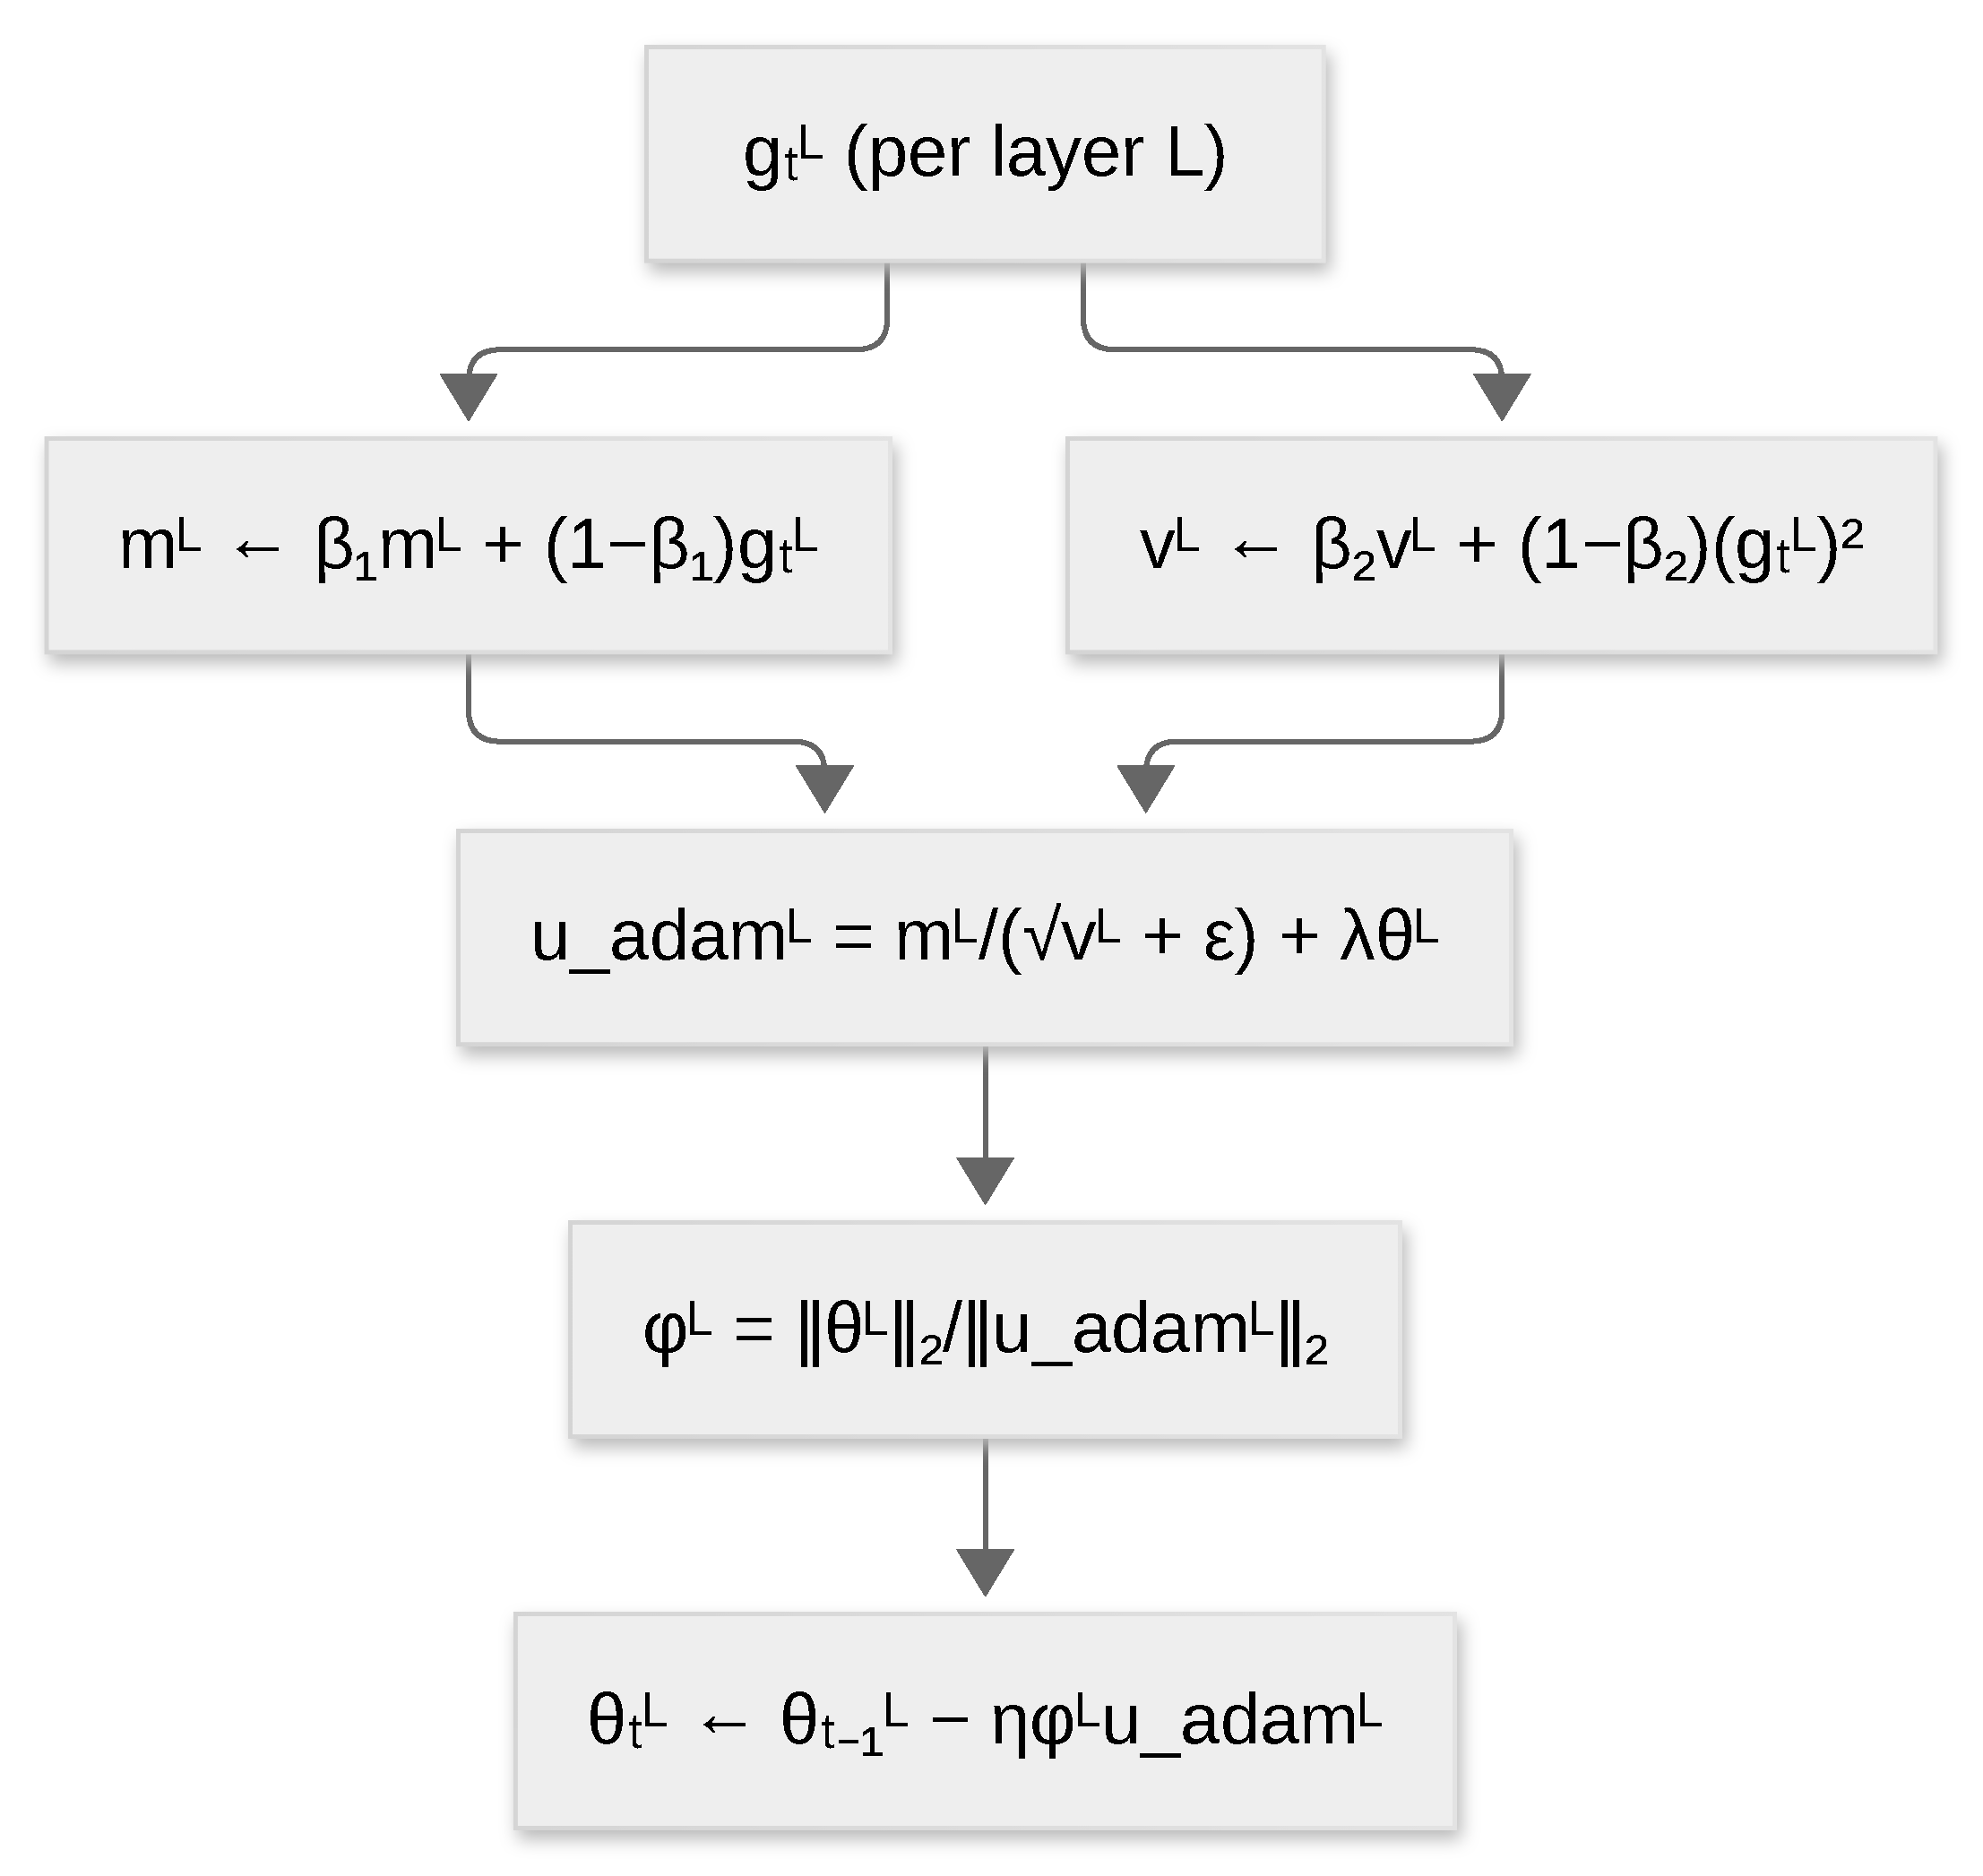
\includegraphics{figures/optimizers/lamb.pdf}}
\caption{Step flow of LAMB: per-layer Adam step rescaled by the trust ratio between weight and update norms.}
\label{fig:opt-lamb}
\end{figure}
LAMB extends Adam with \textbf{layer-wise adaptive rate scaling} (inspired by LARS), enabling stable training with extreme batch sizes (e.g., 64K on BERT):
\begin{align}
m_t^L &= \beta_1 m_{t-1}^L + (1-\beta_1)g_t^L \quad\text{(layer-wise first moment)} \\
v_t^L &= \beta_2 v_{t-1}^L + (1-\beta_2)(g_t^L)^2 \\
u_{\text{adam}}^L &= \frac{m_t^L}{\sqrt{v_t^L}+\epsilon} + \lambda\theta_{t-1}^L \quad\text{(base adaptive step with decay)} \\
\phi^L &= \frac{\|\theta_{t-1}^L\|_2}{\|u_{\text{adam}}^L\|_2} \quad\text{(trust ratio: layer normalization)} \\
\theta_t^L &= \theta_{t-1}^L - \eta \cdot \phi^L \cdot u_{\text{adam}}^L
\end{align}
The \textbf{trust ratio} $\phi^L = \|\theta^L\|_2 / \|u_{\text{adam}}^L\|_2$ normalizes the effective update step relative to weight magnitude. In very large batches, stochastic gradient noise can exceed signal, destabilizing layer-wise learning rates. By scaling updates proportionally to weight norms, LAMB ensures relative changes rather than absolute ones, preventing small confident updates in large vectors from dominating.

\begin{algorithm}[H]
\caption{LAMB (Layer-wise Adaptive Moments optimizer for Batch training)}
\label{alg:lamb}
\begin{algorithmic}[1]
\Require Initial parameters $\theta_0$, learning rate $\eta$, $\beta_1, \beta_2$, weight decay $\lambda$
\Ensure Updated parameters $\theta_T$
\State Initialize: For each layer $L$: $m^L \gets 0$, $v^L \gets 0$
\For{$t = 1, 2, \ldots, T$}
    \For{each layer $L$}
        \State $g_t^L \gets \nabla f(\theta_t^L)$
        \State $m^L \gets \beta_1 m^L + (1-\beta_1) g_t^L$
        \State $v^L \gets \beta_2 v^L + (1-\beta_2) (g_t^L)^2$
        \State Base Adam: $u_{\text{adam}}^L \gets m^L / (\sqrt{v^L} + \epsilon)$
        \If{weight\_decay $> 0$}
            \State $u_{\text{adam}}^L \gets u_{\text{adam}}^L + \lambda \theta_{t-1}^L$
        \EndIf
        \State Trust ratio: $\phi^L \gets \|\theta_{t-1}^L\|_2 / \|u_{\text{adam}}^L\|_2$ if both nonzero, else $1$
        \State $\theta_t^L \gets \theta_{t-1}^L - \eta \phi^L u_{\text{adam}}^L$
    \EndFor
\EndFor
\Return $\theta_T$
\end{algorithmic}
\end{algorithm}

\paragraph{Cons.}
\begin{itemize}[leftmargin=*]
\item Layer-wise norm bookkeeping and trust-ratio computation add per-step overhead.
\item The trust ratio is unstable when layer or update norms are close to zero.
\end{itemize}

\paragraph{Pros.}
\begin{itemize}[leftmargin=*]
\item Enables stable training with extreme batch sizes (e.g., 64K on BERT).
\item Preserves small-batch generalization benefits while scaling the batch.
\end{itemize}

\paragraph{Schedule-Free AdamW.}
\begin{figure}[H]
\centering
\fitfigure{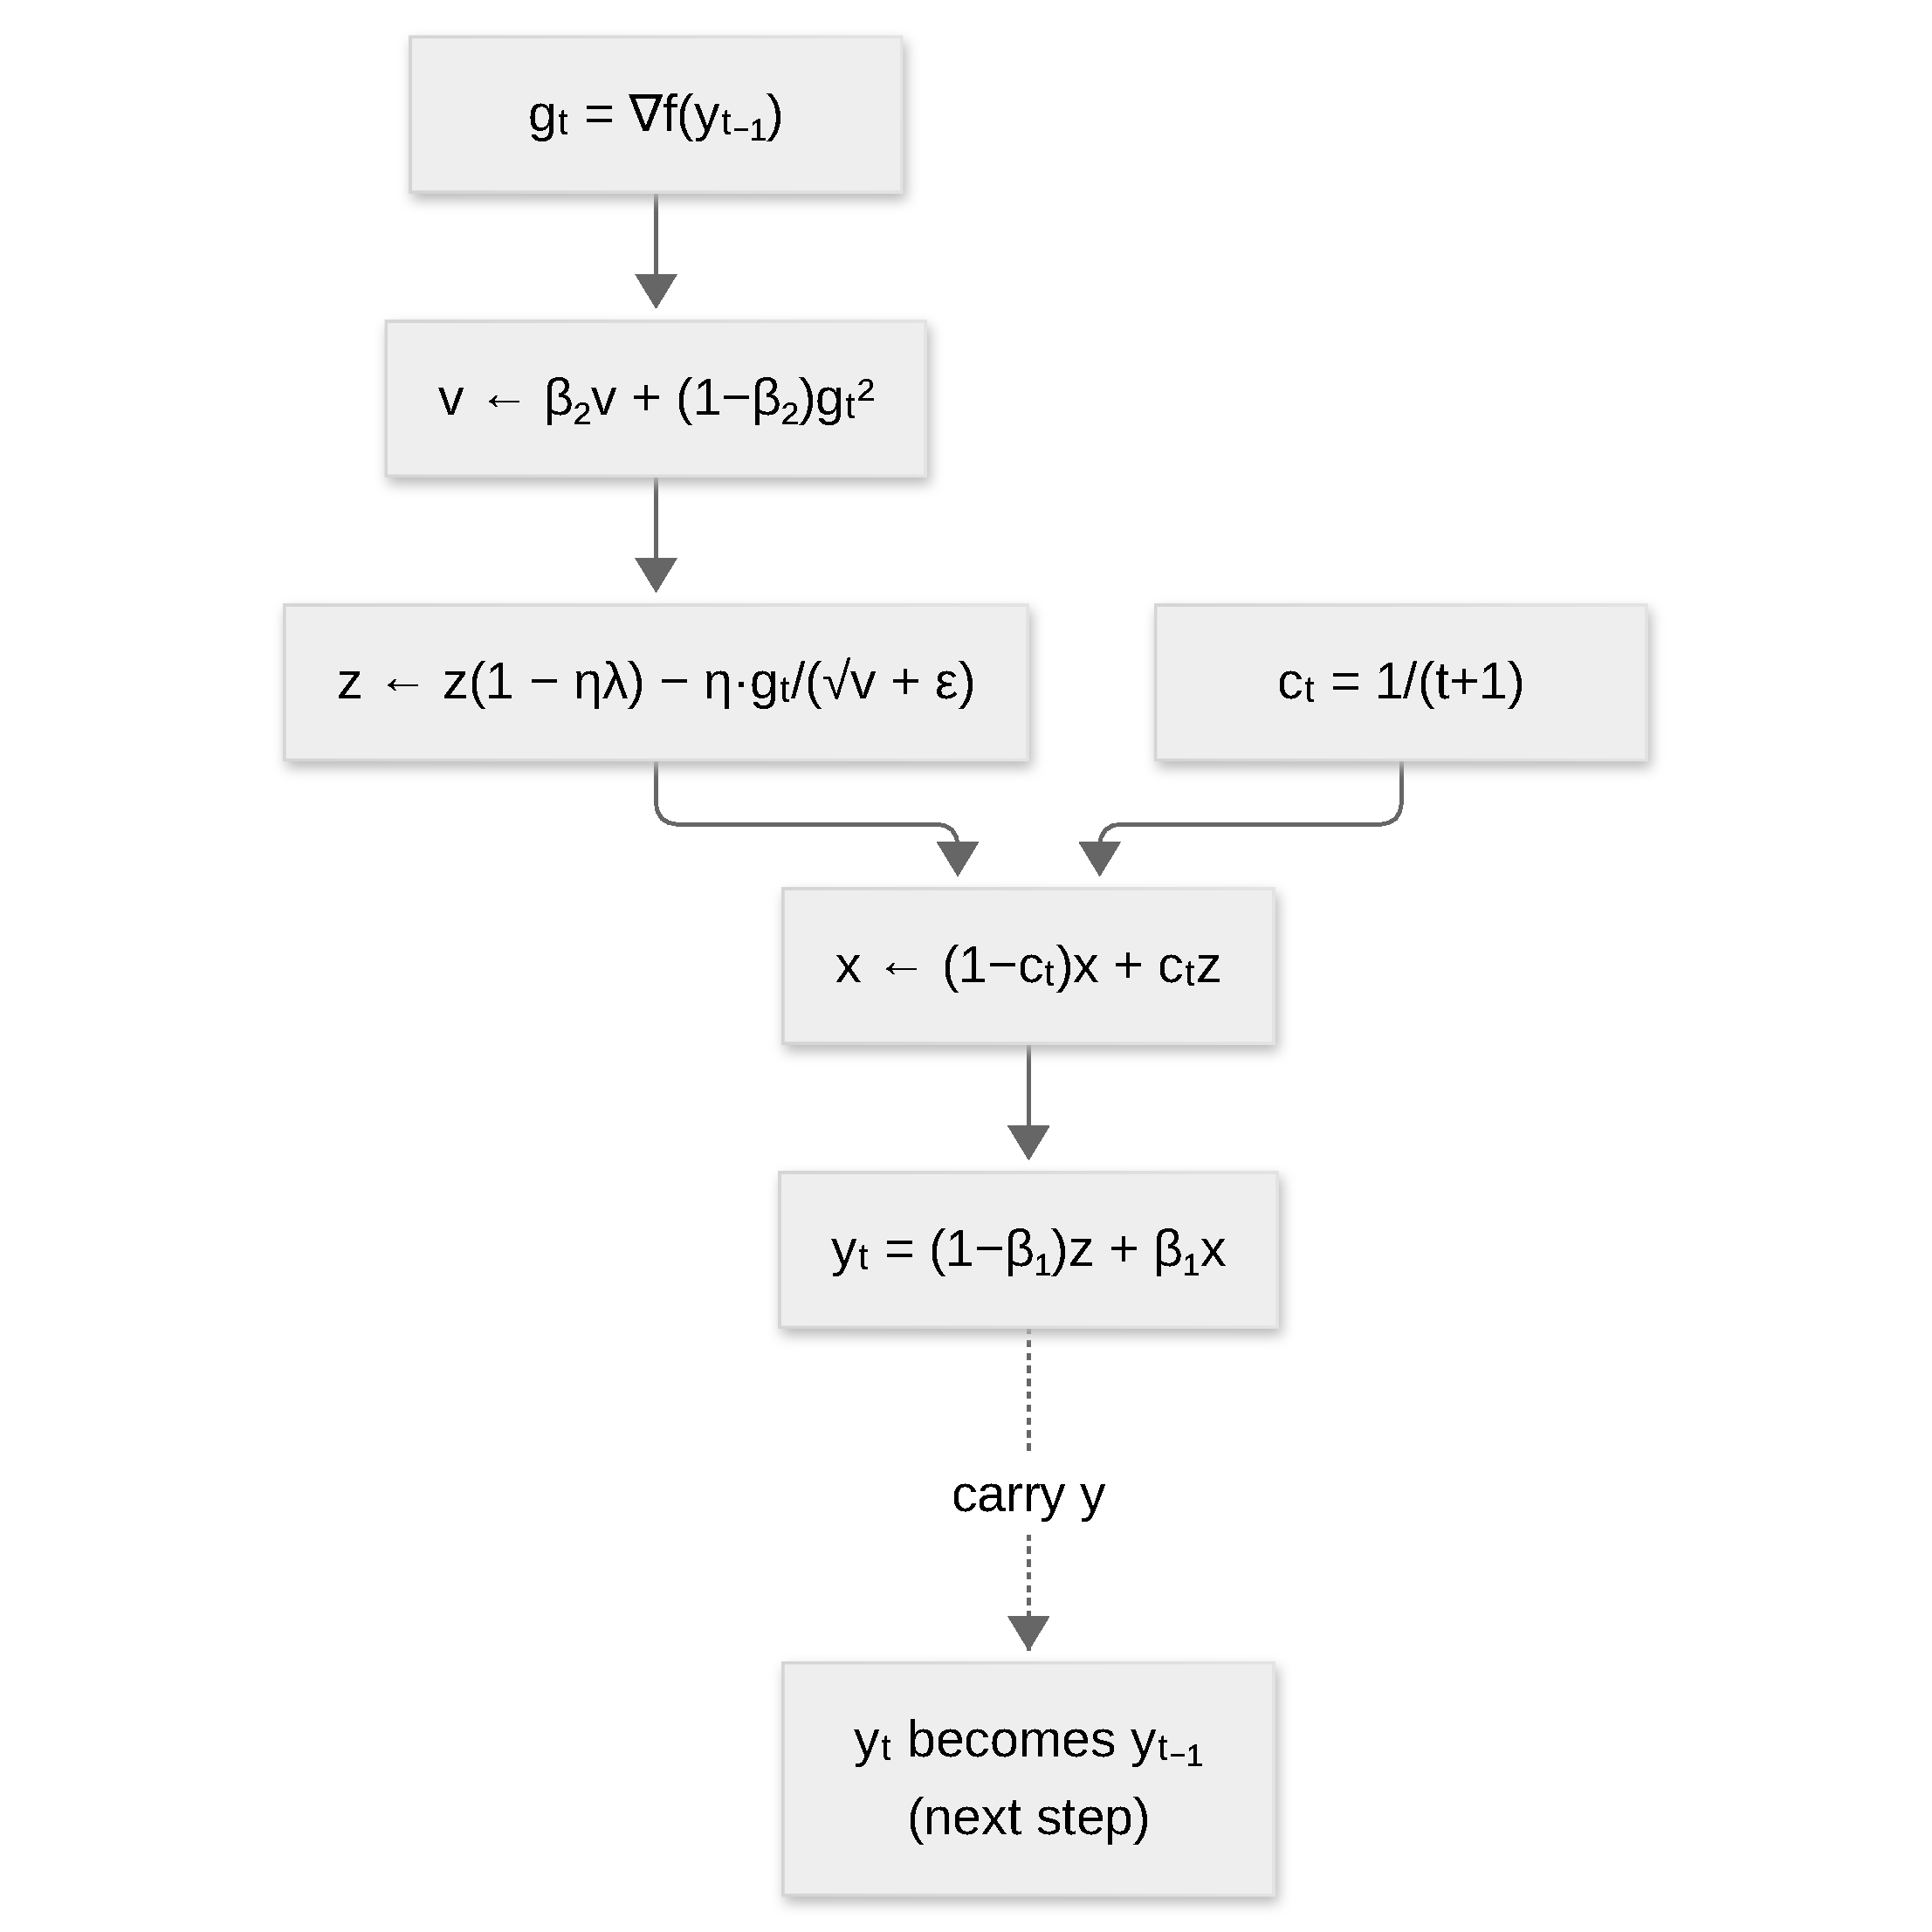
\includegraphics{figures/optimizers/schedulefree.pdf}}
\caption{Step flow of Schedule-Free AdamW: exploration stream $z$, iterate average $x$, and interpolation point $y$, with implicit $1/(t+1)$ averaging.}
\label{fig:opt-schedulefree}
\end{figure}
Schedule-free methods remove explicit scheduler design from the optimization recipe. The algorithm maintains two parameter streams: $z_t$ (exploration) and $x_t$ (smooth average):
\begin{align}
v_t &= \beta_2 v_{t-1} + (1-\beta_2)g_t^2 \quad\text{(variance)} \\
z_t &= z_{t-1}(1-\eta\lambda) - \eta\frac{g_t}{\sqrt{v_t}+\epsilon} \quad\text{(adaptive step with decay)} \\
c_t &= \frac{1}{t+1} \quad\text{(averaging coefficient, decreases over time)} \\
x_t &= (1-c_t)x_{t-1} + c_t z_t \quad\text{(iterate averaging)} \\
y_t &= (1-\beta)z_t + \beta x_t \quad\text{(interpolation for evaluation point)}
\end{align}
The averaging coefficient $c_t = 1/(t+1)$ implements an implicit learning-rate schedule without explicitly specifying total steps $T$. This framework unifies scheduling and iterate averaging: the algorithm explores via $z_t$ while accumulating stable direction via $x_t$. The evaluation point $y_t$ (used for gradient computation) interpolates between exploration and stability.

\begin{algorithm}[H]
\caption{Schedule-Free AdamW}
\label{alg:schedulefree}
\begin{algorithmic}[1]
\Require Initial parameters $\theta_0$, learning rate $\eta$ (fixed), $\beta_1, \beta_2$, weight decay $\lambda$
\Ensure Updated parameters $\theta_T$ or averaging $x_T$
\State Initialize: $z \gets \theta_0$ (exploration), $x \gets \theta_0$ (average), $v \gets 0$, $t \gets 0$
\For{$t = 1, 2, \ldots, T$}
    \State $g_t \gets \nabla f(y_{t-1})$ (gradient at interpolation point)
    \State $v \gets \beta_2 v + (1-\beta_2) g_t^2$ \Comment{Variance}
    \State Weight decay on $z$: $z \gets z(1 - \eta\lambda)$
    \State $z \gets z - \eta g_t / (\sqrt{v} + \epsilon)$ \Comment{Adaptive step on raw}
    \State $c_t \gets 1 / (t+1)$ \Comment{Averaging coefficient}
    \State $x \gets (1-c_t) x + c_t z$ \Comment{Iterate averaging}
    \State $y_t \gets (1-\beta_1) z + \beta_1 x$ \Comment{Interpolation for next eval}
\EndFor
\Return $x_T$ or $y_T$
\end{algorithmic}
\end{algorithm}

\paragraph{Cons.}
\begin{itemize}[leftmargin=*]
\item Maintains two parameter streams ($z$ and $x$) and requires explicit handling of the evaluation point.
\item Behavior departs from scheduled baselines, which complicates comparisons.
\end{itemize}

\paragraph{Pros.}
\begin{itemize}[leftmargin=*]
\item Removes the explicit learning-rate schedule and its total-step hyperparameter.
\item State-of-the-art convergence across convex optimization, large-scale deep learning, and reinforcement learning.
\end{itemize}

\paragraph{Adafactor.}
\begin{figure}[H]
\centering
\fitfigure{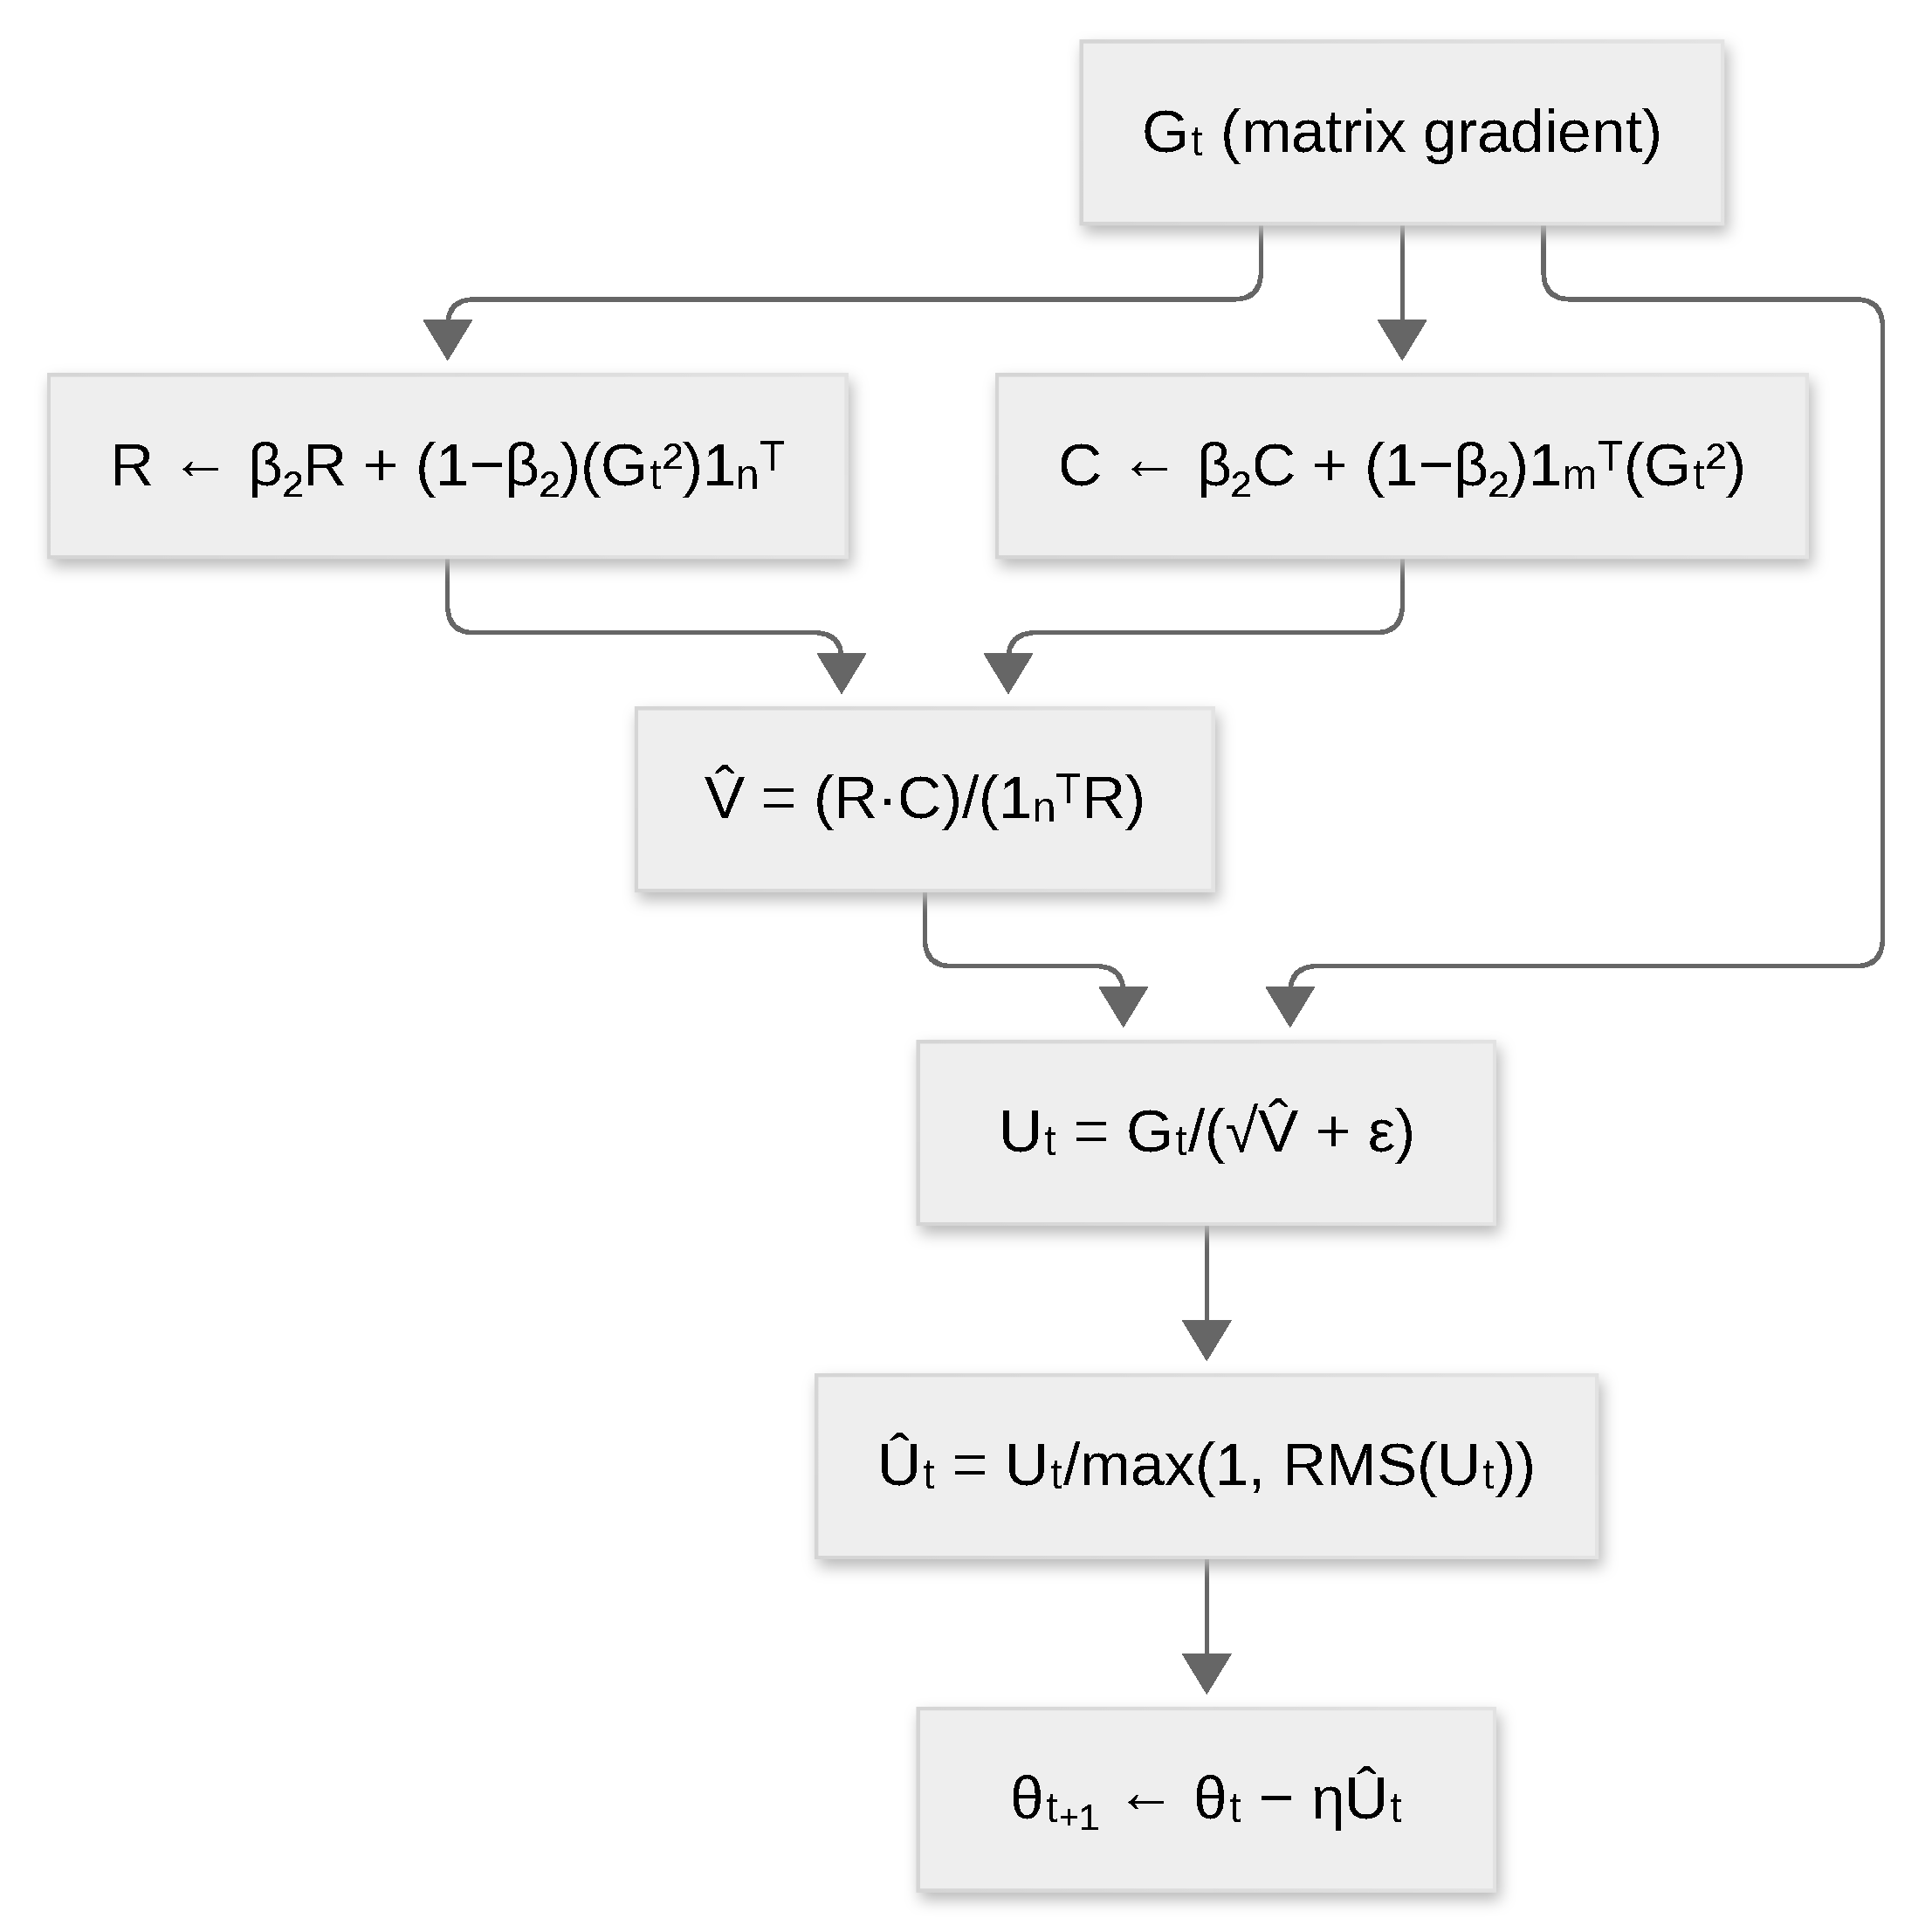
\includegraphics{figures/optimizers/adafactor.pdf}}
\caption{Step flow of Adafactor: factorized row/column second-moment accumulators, outer-product variance reconstruction, and RMS clipping.}
\label{fig:opt-adafactor}
\end{figure}
Adafactor reduces optimizer memory by \textbf{factorizing} second-moment statistics for matrix-shaped parameters, storing only row and column accumulators rather than dense variance states. For a gradient matrix $G_t \in \mathbb{R}^{m \times n}$:
\begin{align}
R_t &= \beta_2 R_{t-1} + (1-\beta_2)(G_t^2) \mathbf{1}_n^T \quad\text{(row variance)} \\
C_t &= \beta_2 C_{t-1} + (1-\beta_2) \mathbf{1}_m^\top (G_t^2) \quad\text{(column variance)} \\
\hat{V}_t &= \frac{R_t C_t}{\mathbf{1}_n^\top R_t} \quad\text{(reconstructed variance via outer product)} \\
U_t &= \frac{G_t}{\sqrt{\hat{V}_t}+\epsilon} \quad\text{(normalized adaptive step)} \\
\hat{U}_t &= \frac{U_t}{\max(1, \text{RMS}(U_t))} \quad\text{(stability clipping)}
\end{align}

\begin{algorithm}[H]
\caption{Adafactor (Factorized Second-Moment Statistics)}
\label{alg:adafactor}
\begin{algorithmic}[1]
\Require Gradient matrix $G_t \in \mathbb{R}^{m \times n}$, learning rate $\eta$, $\beta_2 \approx 0.999$
\Ensure Updated parameters $\theta_T$
\State Initialize: Row accumulators $R \gets \epsilon \mathbf{1}^T_m$, Column $C \gets \epsilon \mathbf{1}_n$
\For{$t = 1, 2, \ldots, T$}
    \State $G_t \gets \nabla f(\theta_t)$ (matrix gradient)
    \State $R \gets \beta_2 R + (1-\beta_2) (G_t^2) \mathbf{1}_n^T$ \Comment{Row inner products}
    \State $C \gets \beta_2 C + (1-\beta_2) \mathbf{1}_m^\top (G_t^2)$ \Comment{Column inner products}
    \State Reconstructed variance: $\hat{V} \gets (R \cdot C) / (\mathbf{1}_n^\top R)$ \Comment{Via outer product}
    \State Normalized adaptive step: $U_t \gets G_t / (\sqrt{\hat{V}} + \epsilon)$
    \State Per-row RMS clipping: $\hat{U}_t \gets U_t / \max(1, \text{RMS}(U_t))$
    \State $\theta_{t+1} \gets \theta_t - \eta \hat{U}_t$
\EndFor
\Return $\theta_T$
\end{algorithmic}
\end{algorithm}

\paragraph{Cons.}
\begin{itemize}[leftmargin=*]
\item Factorized variance is an approximation and can be unstable on some tasks.
\item Reduced optimization expressiveness relative to full Adam.
\end{itemize}

\paragraph{Pros.}
\begin{itemize}[leftmargin=*]
\item Memory drops from $O(n_{\text{params}})$ to $O(\sqrt{n_{\text{params}}})$ for matrix parameters.
\item Most attractive when VRAM is dominated by optimizer state rather than activations.
\end{itemize}

\paragraph{GaLore (Gradient Low-Rank Projection).}
\begin{figure}[H]
\centering
\fitfigure{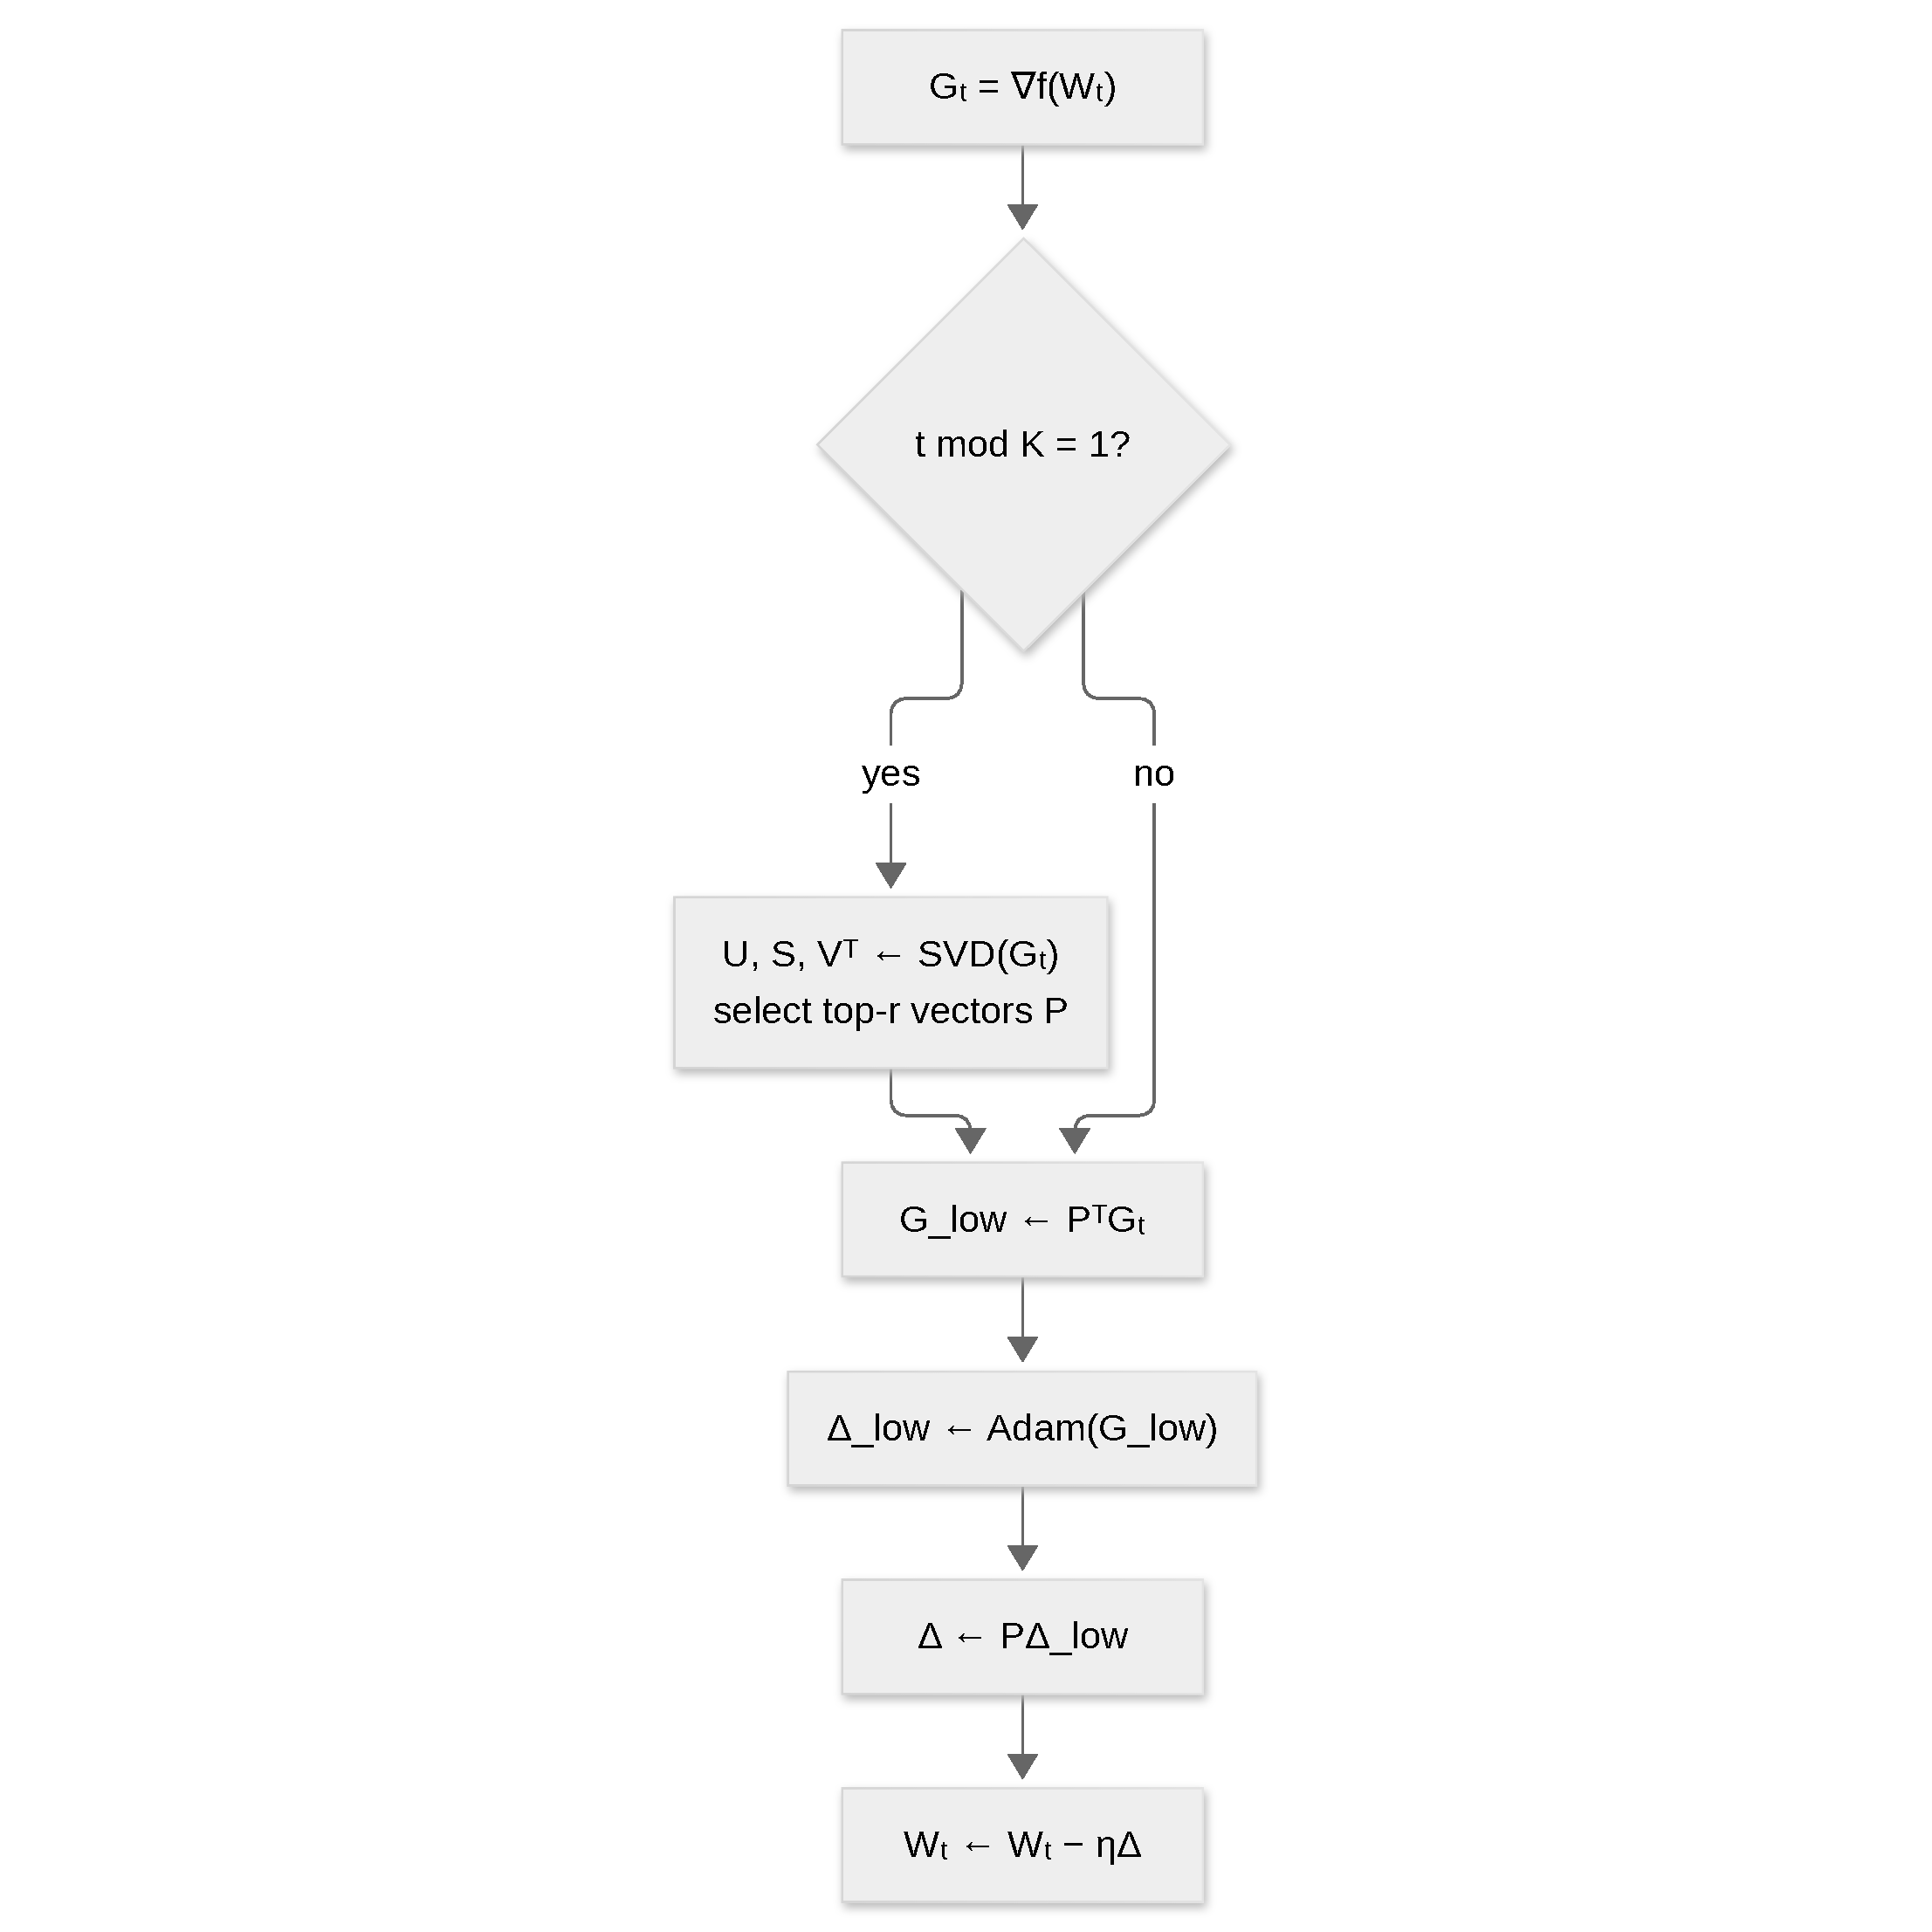
\includegraphics{figures/optimizers/galore.pdf}}
\caption{Step flow of GaLore: periodic SVD projection of the gradient into a low-rank subspace, Adam in that subspace, and reconstruction.}
\label{fig:opt-galore}
\end{figure}
GaLore projects 2D gradients into a low-rank subspace before optimization, reducing optimizer-state memory while maintaining adaptive step scaling. For a 2D parameter matrix $W \in \mathbb{R}^{m \times n}$:
\begin{align}
U, S, V &= \text{SVD}(G_t) \quad\text{(compute singular decomposition)} \\
P &\in \mathbb{R}^{n \times r} \quad\text{or} \quad P^\top \in \mathbb{R}^{r \times m} \quad\text{(select top-$r$ singular vectors)} \\
G_{\text{low}} &= P^\top G_t \quad\text{(project to low-rank space)} \\
\Delta_{\text{low}} &= \text{Adam}(G_{\text{low}}) \quad\text{(optimize in compressed space)} \\
\Delta &= P \Delta_{\text{low}} \quad\text{(reconstruct in original space)}
\end{align}
By projecting into a rank-$r$ subspace (typically $r \ll \min(m,n)$), optimizer state is reduced from $O(mn)$ to $O(r(m+n))$ for 2D parameters. This complementary memory-saving approach is especially relevant when the model is too large for full-rank optimizer state.

\begin{algorithm}[H]
\caption{GaLore (Gradient Low-Rank Projection)}
\label{alg:galore}
\begin{algorithmic}[1]
\Require 2D parameter matrix $W \in \mathbb{R}^{m \times n}$, learning rate $\eta$, rank $r \ll \min(m,n)$
\Ensure Updated parameters $\theta_T$
\State Initialize: Adam state in low-rank space (if rank-2 variant)
\For{$t = 1, 2, \ldots, T$}
    \State $G_t \gets \nabla f(W_t)$
    \If{$t \mod K = 1$}  \Comment{Periodic SVD}
        \State $U_t, S_t, V_t^\top \gets \text{SVD}(G_t)$ (full or thin)
        \State Select projection: $P \gets U_t[:, :r]$ or $P \gets V_t[:, :r]$
    \EndIf
    \State Project gradient: $G_{\text{low}} \gets P^\top G_t$ (or $G_t P^\top$ for right projection)
    \State Run Adam on low-rank: $\Delta_{\text{low}} \gets \text{Adam}(G_{\text{low}})$
    \State Reconstruct in original space: $\Delta \gets P \Delta_{\text{low}}$ (or $\Delta_{\text{low}} P^\top$)
    \State $W_t \gets W_t - \eta \Delta$
\EndFor
\Return $\theta_T$
\end{algorithmic}
\end{algorithm}

\paragraph{Cons.}
\begin{itemize}[leftmargin=*]
\item Periodic SVD adds compute and introduces a projection-refresh interval to tune.
\item Low-rank projection can discard gradient information.
\end{itemize}

\paragraph{Pros.}
\begin{itemize}[leftmargin=*]
\item Optimizer state reduced from $O(mn)$ to $O(r(m+n))$ for 2D parameters.
\item Works synergistically with other techniques and has shown strong results on billion-parameter models.
\end{itemize}

\paragraph{APOLLO, APOLLO-Mini, and Q-APOLLO.}
\begin{figure}[H]
\centering
\fitfigure{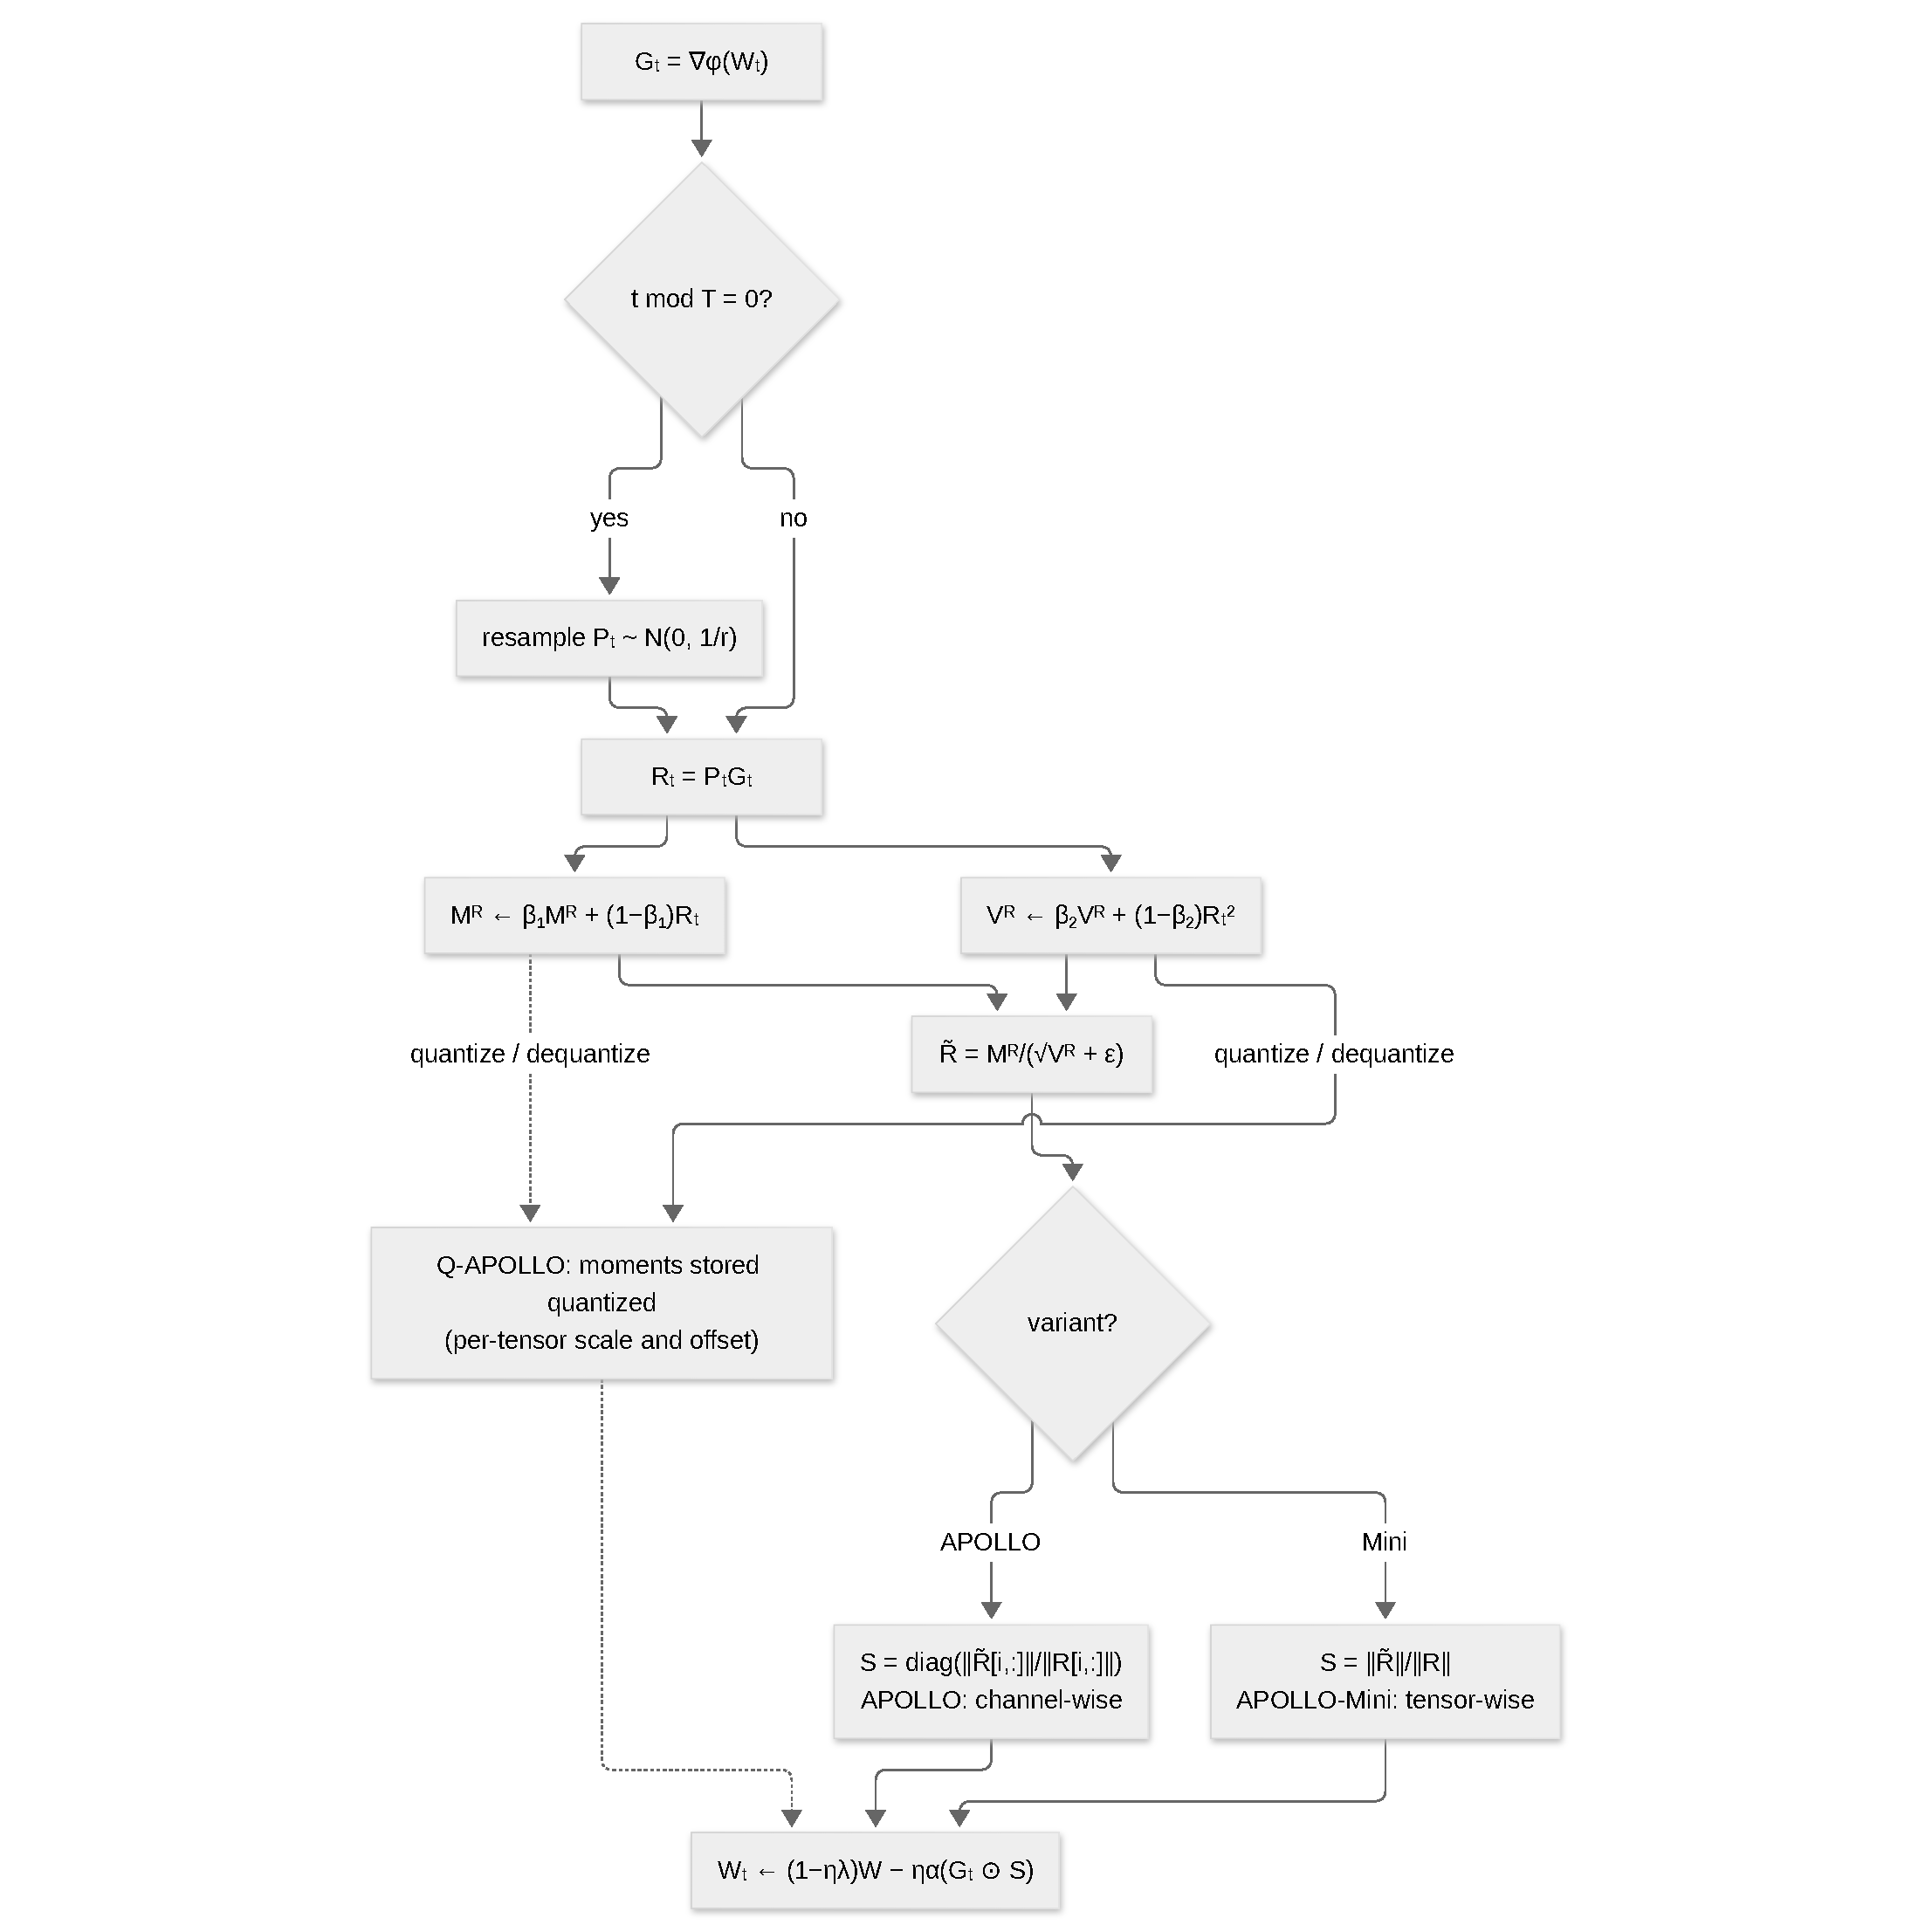
\includegraphics{figures/optimizers/apollo.pdf}}
\caption{Step flow of the APOLLO family: Gaussian-projected moments, structured gradient scaling (channel-wise for APOLLO, scalar for APOLLO-Mini), and quantized state for Q-APOLLO.}
\label{fig:opt-apollo}
\end{figure}
The APOLLO family \citep{zhu2025apollosgdlikememoryadamwlevel} begins from the observation that AdamW's element-wise denominator can be \textbf{coarsened into a structured learning-rate update}. Rather than storing dense moments for every parameter entry, APOLLO projects a matrix gradient $G_t \in \mathbb{R}^{m \times n}$ into a compact random subspace and tracks Adam-style moments there:
\begin{align}
R_t &= P_t G_t \quad\text{or}\quad R_t = G_t P_t^\top \\
M_t^R &= \beta_1 M_{t-1}^R + (1-\beta_1)R_t \\
V_t^R &= \beta_2 V_{t-1}^R + (1-\beta_2)R_t^2 \\
\widetilde{R}_t &= \frac{M_t^R}{\sqrt{V_t^R}+\epsilon}
\end{align}
The projected state is \emph{not} expanded back into a dense low-rank update as in SVD-based methods. Instead, APOLLO estimates a structured scaling tensor $S_t$ in the original space. In the standard APOLLO variant, that scaling is \textbf{channel-wise}: each row or channel receives its own norm ratio. In APOLLO-Mini, the scaling is reduced to a single \textbf{tensor-wise} scalar, corresponding to the rank-1 extreme described in the paper. The resulting parameter update is therefore Adam-like in adaptation but much closer to SGD in state cost:
\[
W_t \gets (1-\eta\lambda)W_{t-1} - \eta\,\alpha\,(G_t \odot S_t)
\]
where $\alpha$ is the extra scale factor used to stabilize highly compressed variants.

\begin{algorithm}[H]
\caption{APOLLO / APOLLO-Mini Structured Gradient Scaling}
\label{alg:apollo-family}
\begin{algorithmic}[1]
\Require Weight matrix $W \in \mathbb{R}^{m \times n}$ with $m \le n$, learning rate $\eta$, scale factor $\alpha$, decay rates $(\beta_1, \beta_2)$, weight decay $\lambda$, rank $r$, projection refresh interval $T$
\Ensure Updated parameters $W_T$
\State Initialize projected moments: $M^R \gets 0$, $V^R \gets 0$, step $t \gets 0$
\Repeat
    \State Compute gradient: $G_t \gets \nabla_W \phi(W_t)$
    \If{$t \bmod T = 0$}
        \State Sample Gaussian projector $P_t \sim \mathcal{N}(0, 1/r)$ with a fresh seed
    \EndIf
    \State Project gradient: $R_t \gets P_t G_t$ \Comment{or $G_t P_t^\top$ depending on layout}
    \State Update projected AdamW moments: $M_t^R, V_t^R \gets \text{AdamWState}(R_t; \beta_1, \beta_2)$
    \State Normalize projected state: $\widetilde{R}_t \gets M_t^R / (\sqrt{V_t^R}+\epsilon)$
    \If{APOLLO}
        \State $S_t \gets \operatorname{diag}(s_1^R, \ldots, s_m^R)$, where $s_i^R = \|\widetilde{R}_t[i,:]\|_2 / \|R_t[i,:]\|_2$
    \Else
        \State $S_t \gets s_t^R$, where $s_t^R = \|\widetilde{R}_t\|_2 / \|R_t\|_2$
    \EndIf
    \State Update weights: $W_t \gets (1-\eta\lambda)W_{t-1} - \eta\,\alpha\,(G_t \odot S_t)$
    \State $t \gets t+1$
\Until{convergence}
\end{algorithmic}
\end{algorithm}

\paragraph{Cons.}
\begin{itemize}[leftmargin=*]
\item Structured scaling is a coarser approximation of AdamW's element-wise denominator.
\item Projectors must be refreshed periodically, and very small ranks make the scaling noisy.
\end{itemize}

\paragraph{Pros.}
\begin{itemize}[leftmargin=*]
\item Replaces repeated SVD with periodically refreshed Gaussian random projection, so the systems cost is ordinary matrix multiplication rather than spectral decomposition.
\item Unusually tolerant to extreme compression: even APOLLO-Mini, which keeps only rank-1 auxiliary state, remains competitive with or better than AdamW while approaching SGD-level memory.
\end{itemize}

\paragraph{APOLLO-Mini.}
APOLLO-Mini is the family member optimized for \textbf{extreme memory efficiency}. The paper motivates it by arguing that, in a rank-1 compact space, channel-wise scaling becomes too noisy, so the update is coarsened further to a single tensor-wise scale. The loss of granularity is partially offset by the explicit scaling factor $\alpha$ (the paper discusses values such as $128$ in this regime), giving a useful point on the optimization Pareto frontier: very small state, no SVD overhead, and still strong pre-training behavior.

\paragraph{Cons.}
\begin{itemize}[leftmargin=*]
\item A single tensor-wise scale loses channel granularity, and rank-1 state can be noisy.
\item Depends on the extra scale factor $\alpha$ (e.g., $128$) to remain stable.
\end{itemize}

\paragraph{Pros.}
\begin{itemize}[leftmargin=*]
\item Smallest state in the APOLLO family, with no SVD overhead.
\item Strong pre-training behavior at near-SGD memory cost.
\end{itemize}

\paragraph{Q-APOLLO.}
The APOLLO paper also stresses that the family combines naturally with \textbf{quantization} for ultra-low-memory training. This repository turns that systems observation into a concrete optimizer variant, \texttt{q\_apollo}. In the implementation, APOLLO's low-rank first and second moments are stored in quantized form together with per-tensor scales and offsets, and are dequantized only when needed for the next step. Q-APOLLO therefore preserves APOLLO's projected-gradient logic while reducing the precision of the remaining optimizer state.

\paragraph{Cons.}
\begin{itemize}[leftmargin=*]
\item Quantized moments introduce approximation error and dequantization overhead.
\item Requires managing per-tensor scales and offsets.
\end{itemize}

\paragraph{Pros.}
\begin{itemize}[leftmargin=*]
\item Reduces the remaining optimizer state to ultra-low precision.
\item Most aggressive memory-saving member of the local optimizer stack while preserving APOLLO's projected-gradient logic.
\end{itemize}

\paragraph{AdamPM (Pooled-Moment Adam).}
AdamPM~\citep{ji_adampm_2026} is a \textbf{minimal, model-agnostic modification of
Adam}: it keeps the element-wise first moment untouched and compresses only the
second moment by \textbf{group-mean pooling of adjacent entries} along each row
(the default, rows being output features) or each column (the paper's
\emph{AdamPM-col}). For a weight matrix $W \in \mathbb{R}^{m \times n}$ and group
size $s$, every row is partitioned into $q = \lceil n/s \rceil$ groups, the
squared gradient is averaged within each group \emph{before} the exponential
moving average, and only the compressed statistic
$\bar{V}_t \in \mathbb{R}^{m \times q}$ is persisted:
\begin{align}
M_t &= \beta_1 M_{t-1} + (1-\beta_1)\, G_t
     && \text{(first moment, element-wise, Eq.~1)} \\
\bar{S}_t &= \frac{1}{s}\sum_{k=1}^{s}
     \mathrm{reshape}(G_t \odot G_t,\, m, q, s)[:,:,k]
     && \text{(within-group means, Eq.~2)} \\
\bar{V}_t &= \beta_2 \bar{V}_{t-1} + (1-\beta_2)\, \bar{S}_t
     && \text{(compressed second-moment EMA, Eq.~3)} \\
W_t &= W_{t-1} - \eta_t \,
     \frac{M_t/(1-\beta_1^t)}
          {\sqrt{\hat{\bar{V}}_t \otimes \mathbf{1}_{1\times s}} + \epsilon},
\qquad \hat{\bar{V}}_t = \frac{\bar{V}_t}{1-\beta_2^t}
     && \text{(update, Eq.~4)}
\end{align}
When $n$ is not divisible by $s$ the final group is padded with its own mean, so
its statistic averages only the entries it actually contains; $s{=}1$ recovers
Adam exactly, and $s \ge n$ collapses each row (or column) to one scalar, the
paper's \emph{AdamPM-inf} limit. AdamPM pools the second moments of
\textbf{all} weight matrices---embeddings, the LM head, attention and MLP
weights---and treats one-dimensional parameters such as RMSNorm scales as
single-row or single-column matrices, so no parameter group is left on a
fallback path. The persistent state is $mn(1+1/s)$ elements against Adam's
$2mn$.

\begin{algorithm}[H]
\caption{AdamPM (Pooled-Moment Adam)}
\label{alg:adampm}
\begin{algorithmic}[1]
\Require Initial parameters $W_0 \in \mathbb{R}^{m\times n}$, steps $T$, group size $s$, learning rate $\eta_t$, decay rates $\beta_1, \beta_2$, stability constant $\epsilon$
\Ensure Updated parameters $W_T$
\State $t \gets 0$; \ $q \gets \lceil n/s \rceil$ \Comment{Number of groups per row}
\State $M_0 \gets \mathbf{0}_{m\times n}$; \ $\bar{V}_0 \gets \mathbf{0}_{m\times q}$ \Comment{First moment and compressed second moment}
\Repeat
    \State $t \gets t + 1$
    \State $G_t \gets \nabla_W \mathcal{L}(W_{t-1})$ \Comment{Gradient}
    \State $M_t \gets \beta_1 M_{t-1} + (1-\beta_1) G_t$ \Comment{First-moment EMA (Eq.~1)}
    \State $\bar{S}_t \gets \operatorname{mean}_{k}\big(\mathrm{reshape}(G_t \odot G_t, m, q, s)[:,:,k]\big)$ \Comment{Group means (Eq.~2)}
    \State $\bar{V}_t \gets \beta_2 \bar{V}_{t-1} + (1-\beta_2) \bar{S}_t$ \Comment{Compressed second-moment EMA (Eq.~3)}
    \State $\hat{M}_t \gets M_t/(1-\beta_1^t)$; \ $\hat{\bar{V}}_t \gets \bar{V}_t/(1-\beta_2^t)$ \Comment{Bias corrections}
    \State broadcast $\hat{\bar{V}}_t$ over each group \Comment{Kronecker product with $\mathbf{1}_{1\times s}$}
    \State $W_t \gets W_{t-1} - \eta_t \hat{M}_t / (\sqrt{\hat{\bar{V}}_t} + \epsilon)$ \Comment{Update (Eq.~4)}
\Until{$t = T$ or convergence}
\Return $W_t$
\end{algorithmic}
\end{algorithm}

Empirically, AdamPM matches a carefully tuned Adam on LLaMA pre-training from
60M to 1.3B parameters while cutting second-moment memory by 87.5\% ($s{=}8$)
to 93.75\% ($s{=}16$), with the same pattern on GLUE fine-tuning of RoBERTa-base
and on TinyLLaVA-1B supervised fine-tuning; group sizes between 2 and 8 are
reported as robust, and three or five---not only powers of two---work because
the incomplete final group is averaged over its own entries.
Theorem~3.1 gives a stationarity bound independent of the group size $s$, and
under a relative-noise condition AdamPM attains the same
$\mathcal{O}(\log T/\sqrt{T})$ rate as Adam. Algorithm~1 of the paper defines no
weight decay; this implementation applies the repository's decoupled
\texttt{wd\_*} decay before the adaptive update, and the shared per-group
\texttt{betas}/\texttt{eps} suffixes parameterize the bias corrections and the
denominator.

\paragraph{Cons.}
\begin{itemize}[leftmargin=*]
\item The diagonal preconditioner becomes coarser as $s$ grows; the paper's
      AdamPM-inf limit shows a measurable perplexity loss at 350M and 1.3B.
\item The saving covers optimizer state only: the first moment stays full-size,
      so optimizer memory is $1+1/s$ of Adam's, not $1/s$.
\item Pooling is one-dimensional (rows or columns); two-dimensional groups and
      selective per-layer pooling remain unexplored (paper limitations).
\end{itemize}

\paragraph{Pros.}
\begin{itemize}[leftmargin=*]
\item Roughly halves optimizer-state memory at the default $s{=}8$ (second
      moment at $1/8$) with Adam-level perplexity through 1.3B parameters and
      negligible per-step overhead---no SVD, no projection, no extra state.
\item Inherits Adam's learning rate and decay rates directly, so existing Adam
      presets transfer without retuning and $\beta_1{=}0.9$, $\beta_2{=}0.95$
      match the repository defaults.
\item Model-agnostic and applies uniformly to every parameter group; the
      preconditioned updates grow more similar to Adam's as model scale grows.
\end{itemize}

\paragraph{Anon (Adaptivity Non-restricted Optimizer with Novel convergence technique).}
\begin{figure}[H]
\centering
\fitfigure{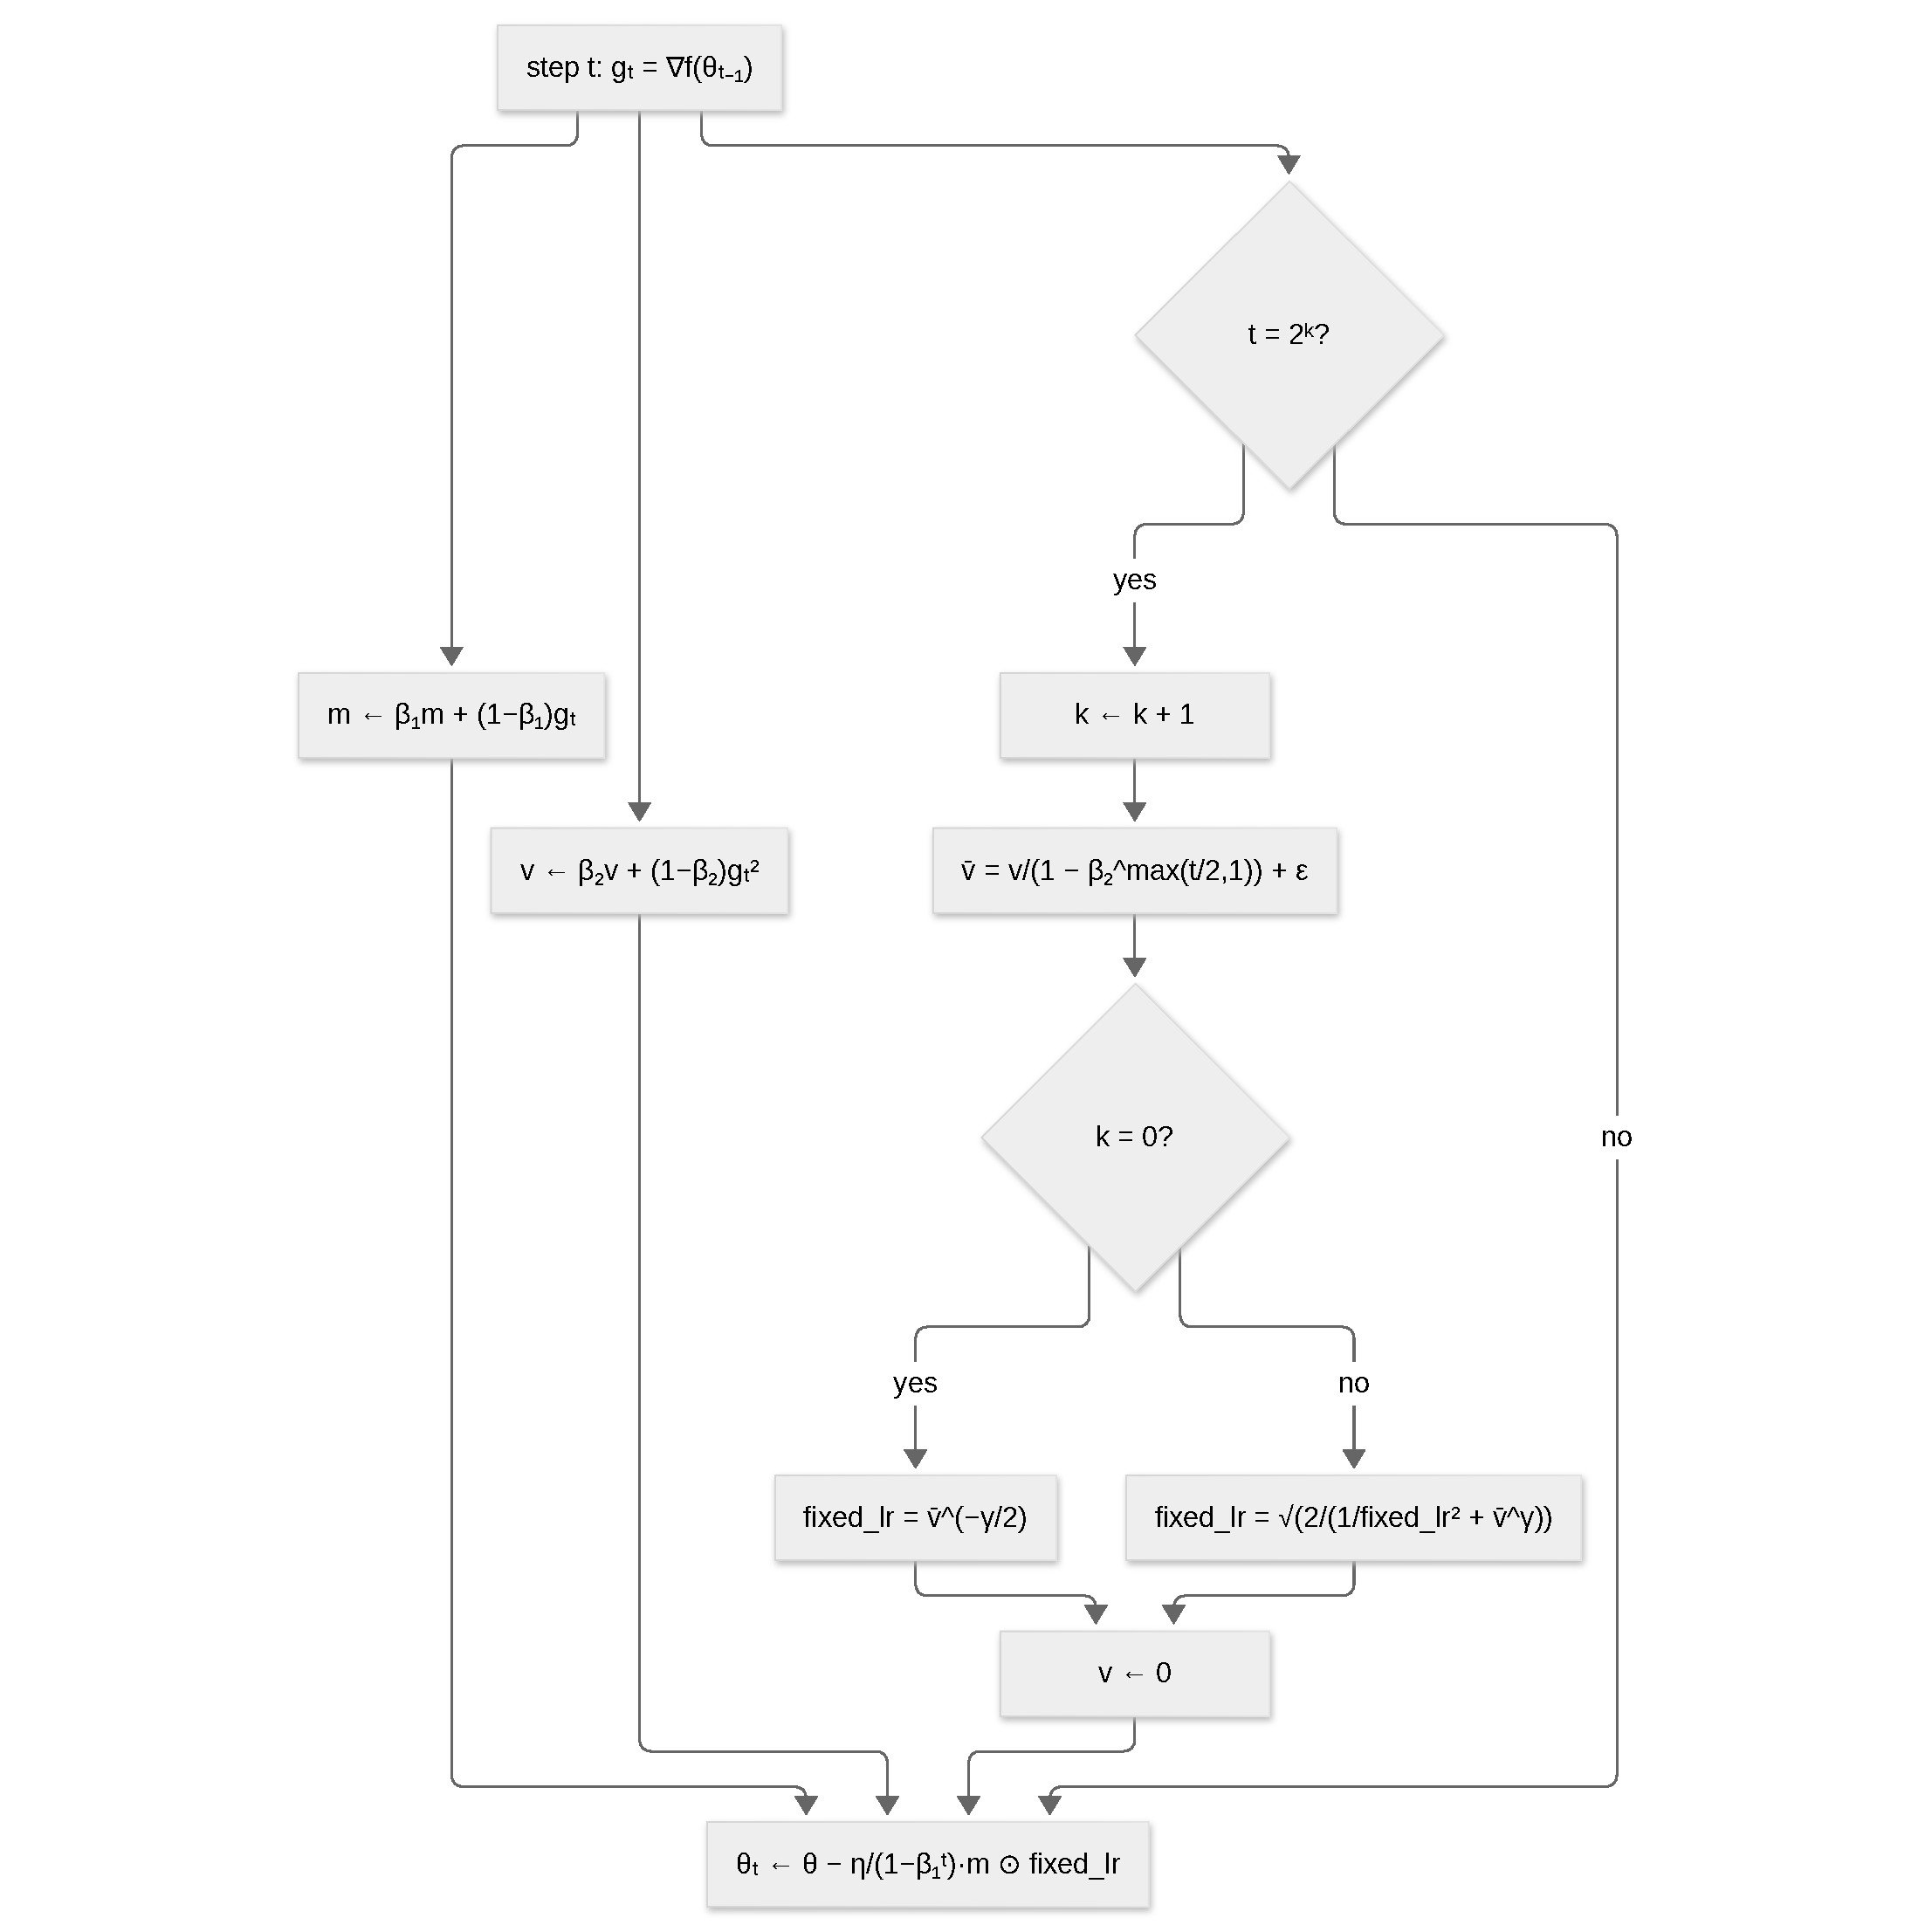
\includegraphics{figures/optimizers/anon.pdf}}
\caption{Step flow of Anon: the IDU preconditioner refreshed at powers of two, with tunable adaptivity $\gamma$ and a bias-corrected momentum update.}
\label{fig:opt-anon}
\end{figure}
Anon \citep{anon2026anon} introduces continuously tunable adaptivity via a single parameter $\gamma \in \mathbb{R}$, bridging the gap between SGD-like ($\gamma=0$) and Adam-like ($\gamma=1$) behaviors, and extrapolating beyond both. The core innovation is the Incremental Delay Update (IDU) mechanism, which enables stable convergence across the entire real-valued adaptivity spectrum:

\begin{align}
m_t &= \beta_1 m_{t-1} + (1-\beta_1) g_t \quad\text{(first moment)}\\
v_t &= \beta_2 v_{t-1} + (1-\beta_2) g_t^2 \quad\text{(second moment)}\\
\bar{v}_t &= \frac{v_t}{1-\beta_2^{\max(t,1)}} + \epsilon \quad\text{(bias-corrected second moment)}\\
\text{fixed\_lr}_k &= \begin{cases}
\bar{v}_k^{-\gamma/2} & \text{if } k = 0 \\
\sqrt{2 / \left(\frac{1}{\text{fixed\_lr}_{k-1}^2} + \bar{v}_k^\gamma\right)} & \text{if } k > 0
\end{cases}\\
\theta_{t+1} &= \theta_t - \frac{\eta}{1-\beta_1^t} \cdot m_t \odot \text{fixed\_lr}_{\lfloor\log_2 t\rfloor}
\end{align}

Unlike standard adaptive optimizers, IDU updates the preconditioner only at powers of two ($t = 2^k$), accumulating gradient statistics between updates and aggregating them recursively. This soft, multi-scale accumulator avoids the hard max-tracking of AMSGrad while provably stabilizing convergence for any $\gamma \in \mathbb{R}$. The parameter $\gamma$ directly controls adaptivity: $\gamma > 1$ accelerates escape from saddle points (favorable for complex architectures), $\gamma = 1$ recovers Adam-like behavior, $\gamma = 0$ yields SGD-like scaling, and $\gamma < 0$ biases toward flatter minima (beneficial for classical architectures like CNNs).

\begin{algorithm}[H]
\caption{Anon (Adaptivity Non-restricted Optimizer with IDU)}
\label{alg:anon}
\begin{algorithmic}[1]
\Require Initial parameters $\theta_0$, learning rate $\eta$, $\beta_1, \beta_2$, tolerance $\epsilon$, adaptivity $\gamma \in \mathbb{R}$
\Ensure Updated parameters $\theta_T$
\State Initialize: $m \gets 0$, $v \gets 0$, fixed\_lr $\gets 0$, step $t \gets 0$, IDU counter $k \gets -1$
\For{$t = 1, 2, \ldots, T$}
    \State $g_t \gets \nabla f(\theta_{t-1})$
    \State $m \gets \beta_1 m + (1-\beta_1) g_t$
    \State $v \gets \beta_2 v + (1-\beta_2) g_t^2$
    \If{$t = 2^k$}
        \State $k \gets k+1$
        \State $\bar{v} \gets v/(1 - \beta_2^{\max(t/2,1)}) + \epsilon$
        \If{$k = 0$}
            \State fixed\_lr $\gets \bar{v}^{-\gamma/2}$
        \Else
            \State fixed\_lr $\gets \sqrt{2 / (1/\text{fixed\_lr}^2 + \bar{v}^\gamma)}$
        \EndIf
        \State $v \gets 0$
    \EndIf
    \State $\theta_t \gets \theta_{t-1} - \frac{\eta}{1-\beta_1^t} \cdot m \odot \text{fixed\_lr}$
\EndFor
\Return $\theta_T$
\end{algorithmic}
\end{algorithm}

\paragraph{Cons.}
\begin{itemize}[leftmargin=*]
\item Maintains three state buffers ($m$, $v$, fixed\_lr) and refreshes the preconditioner on a logarithmic schedule.
\item The adaptivity parameter $\gamma$ must be selected per architecture.
\end{itemize}

\paragraph{Pros.}
\begin{itemize}[leftmargin=*]
\item Same $\mathcal{O}(n)$ per-step complexity class as AdamW, with continuously tunable adaptivity.
\item IDU provably attains $\mathcal{O}(\sqrt{T})$ regret for convex problems and $\mathcal{O}(\ln T / \sqrt{T})$ for non-convex settings.
\end{itemize}

\paragraph{Prodigy (Approximating the Distance Estimate).}
\begin{figure}[H]
\centering
\fitfigure{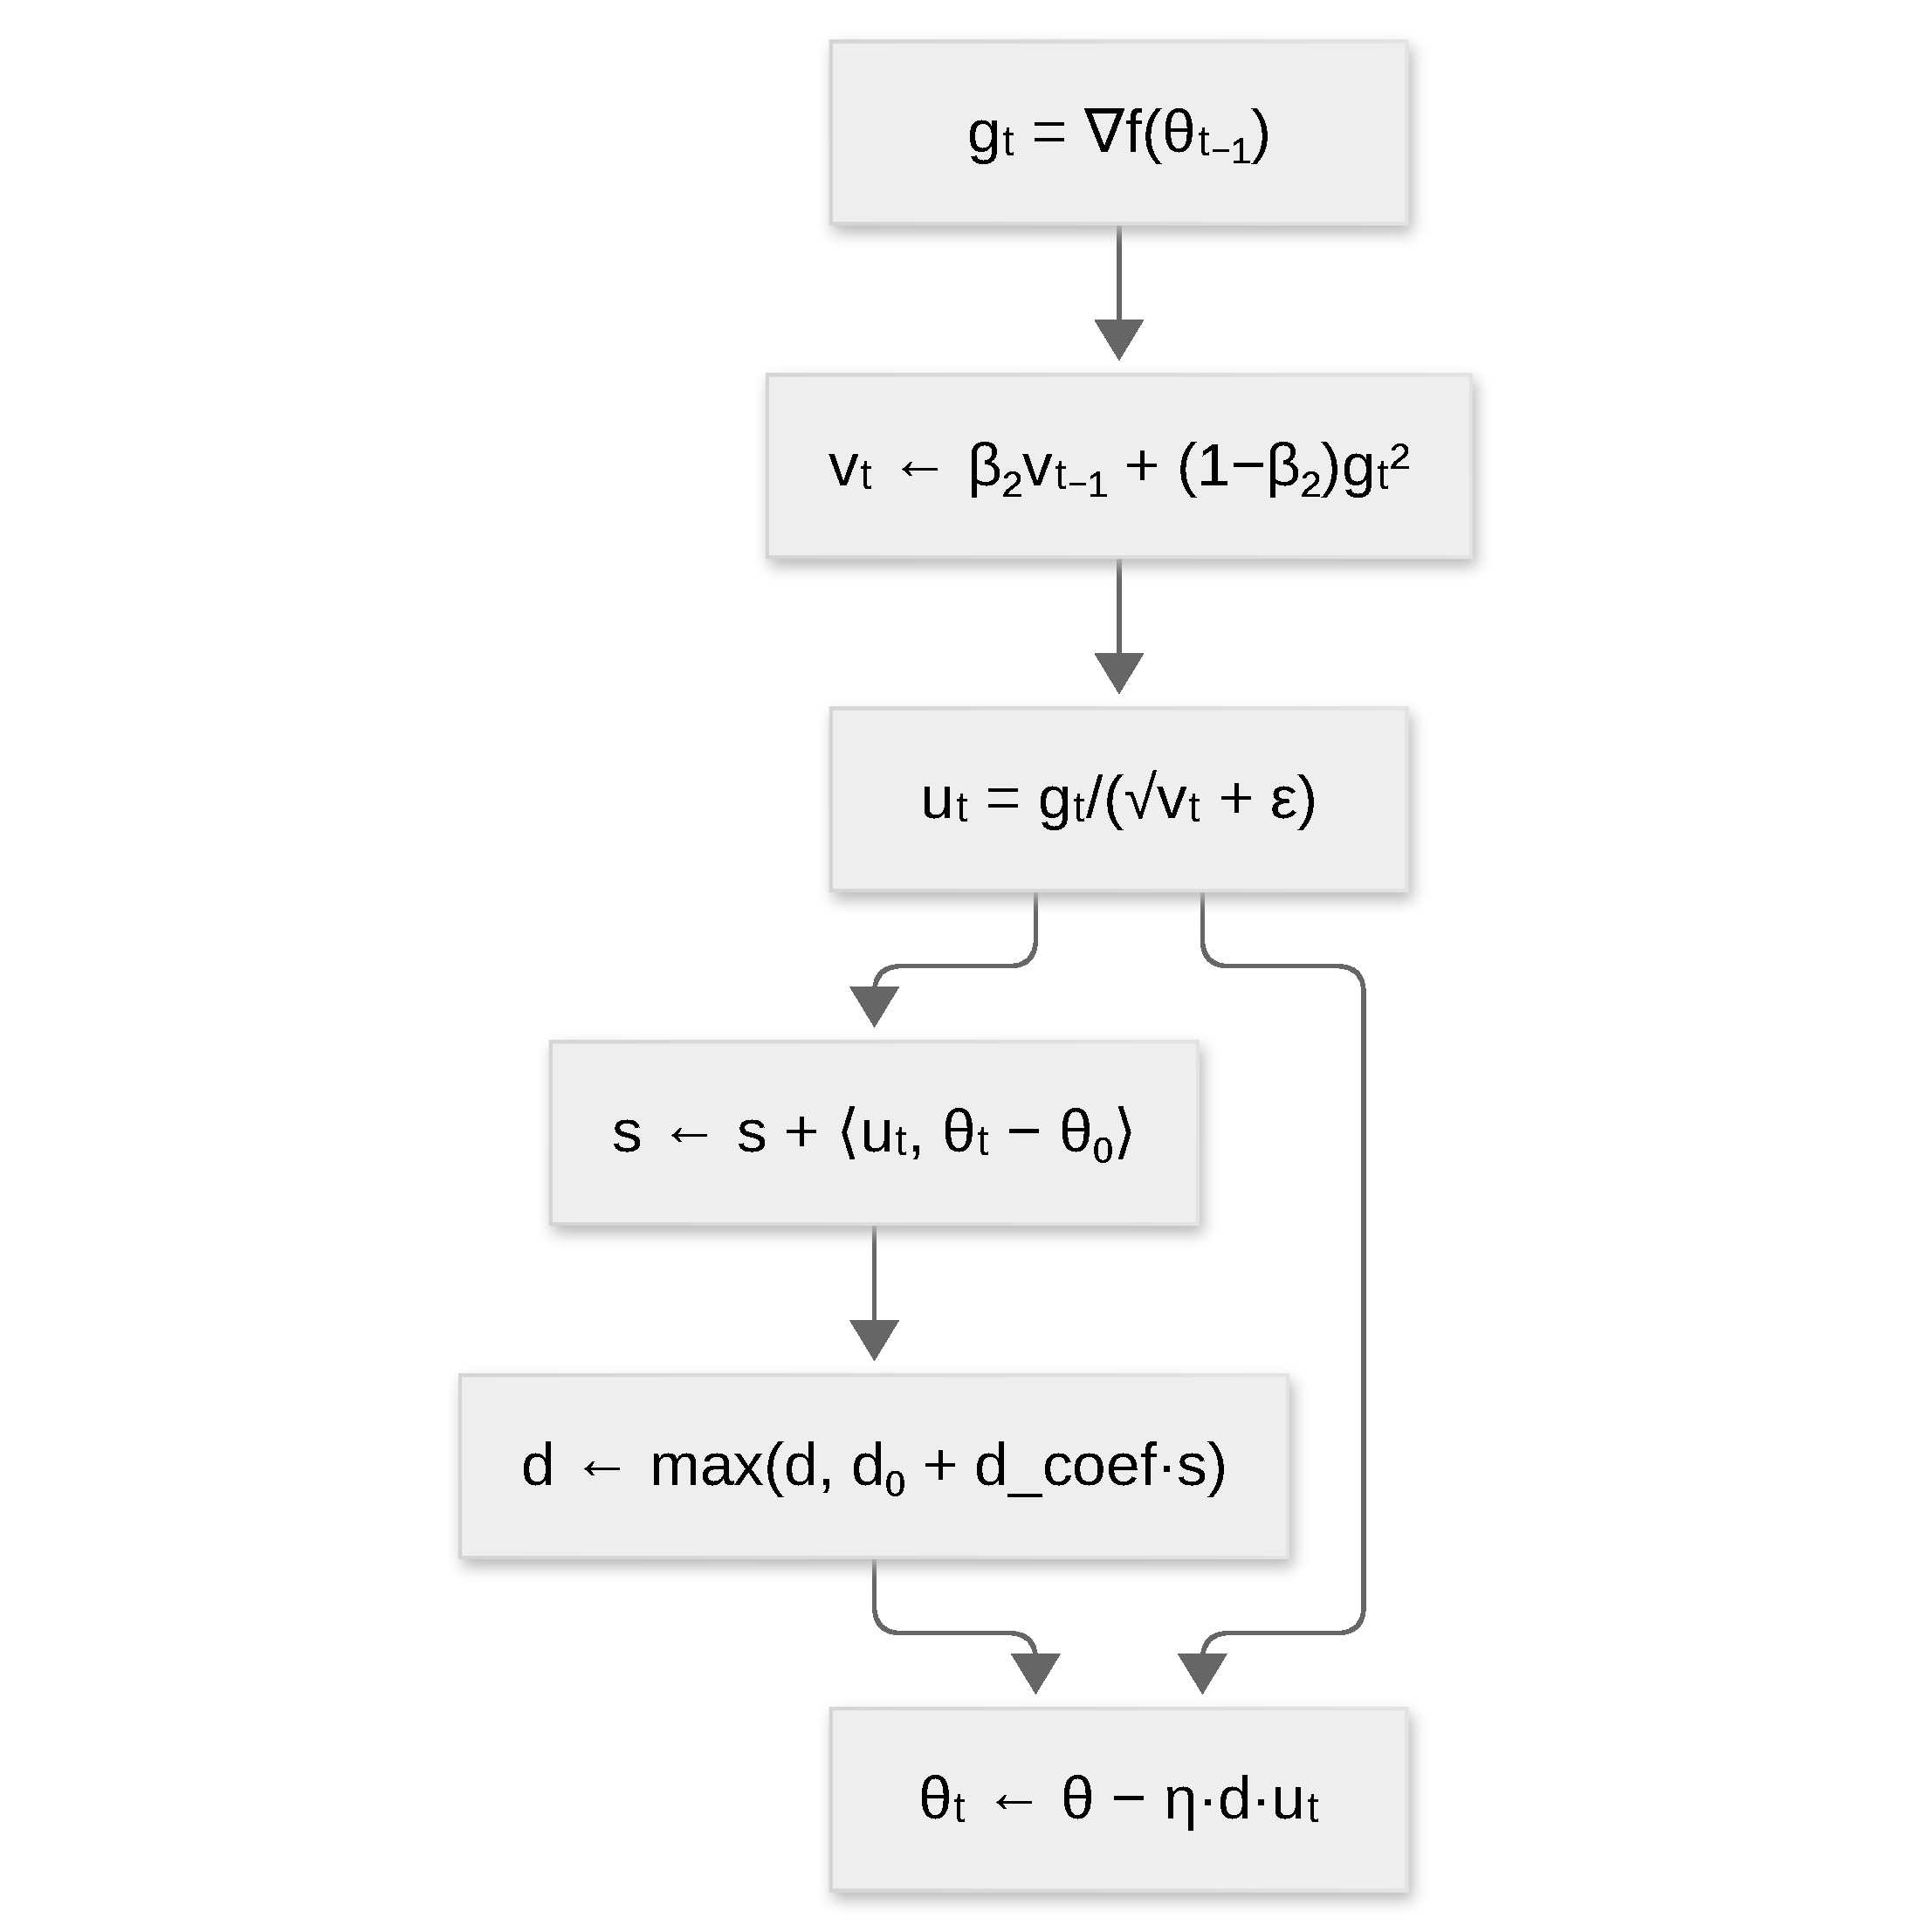
\includegraphics{figures/optimizers/prodigy.pdf}}
\caption{Step flow of Prodigy: a cumulative signed-distance estimate that scales the adaptive step without a learning-rate schedule.}
\label{fig:opt-prodigy}
\end{figure}
Prodigy adapts the effective step scale through a running distance-like statistic, eliminating the need for explicit learning-rate tuning. The algorithm maintains a cumulative distance estimate:
\begin{align}
u_t &= \frac{g_t}{\sqrt{v_t}+\epsilon} \quad\text{(unnormalized adaptive step)} \\
s_t &= s_{t-1} + \langle u_t, \theta_t - \theta_0 \rangle \quad\text{(cumulative signed distance)} \\
d_t &= \max(d_{t-1}, d_0 + d_{\text{coef}} \cdot s_t) \quad\text{(distance estimate with lower bound)} \\
\theta_{t+1} &= \theta_t - \eta \cdot d_t \cdot u_t
\end{align}
where $d_0$ is an initial bound and $d_{\text{coef}}$ controls how aggressively the estimate adapts. The distance estimate $d_t$ captures the combined magnitude of past gradients weighted by actual parameter displacement, implementing an implicit effective learning rate.

\begin{algorithm}[H]
\caption{Prodigy (Approximating the Distance Estimate)}
\label{alg:prodigy}
\begin{algorithmic}[1]
\Require Initial parameters $\theta_0$, learning rate $\eta$, coeff $d_{\text{coef}}$, initial dist $d_0 > 0$
\Ensure Updated parameters $\theta_T$
\State Initialize: $s \gets 0$ (cumulative signed distance), $d \gets d_0$
\For{$t = 1, 2, \ldots, T$}
    \State $g_t \gets \nabla f(\theta_{t-1})$
    \State $v_t \gets \beta_2 v_{t-1} + (1-\beta_2) g_t^2$ \Comment{Second moment}
    \State $u_t \gets g_t / (\sqrt{v_t} + \epsilon)$ \Comment{Unnormalized adaptive}
    \State Update distance: $s \gets s + \langle u_t, \theta_t - \theta_0 \rangle$ \Comment{Signed distance}
    \State $d \gets \max(d, d_0 + d_{\text{coef}} \cdot s)$ \Comment{Lower-bounded distance}
    \State $\theta_t \gets \theta_{t-1} - \eta \cdot d \cdot u_t$ \Comment{Distance-scaled update}
\EndFor
\Return $\theta_T$
\end{algorithmic}
\end{algorithm}

\paragraph{Cons.}
\begin{itemize}[leftmargin=*]
\item Introduces $d_0$ and $d_{\text{coef}}$ hyperparameters for the distance estimate.
\item Adds an inner-product bookkeeping step per iteration.
\end{itemize}

\paragraph{Pros.}
\begin{itemize}[leftmargin=*]
\item Removes explicit learning-rate tuning and scheduling.
\item Robust convergence across problem scales and batch sizes.
\end{itemize}


\subsection{Second-Order, Geometric, and Orthogonality Optimizers}
\paragraph{Shampoo (Matrix Preconditioning via Kronecker Products).}
\begin{figure}[H]
\centering
\fitfigure{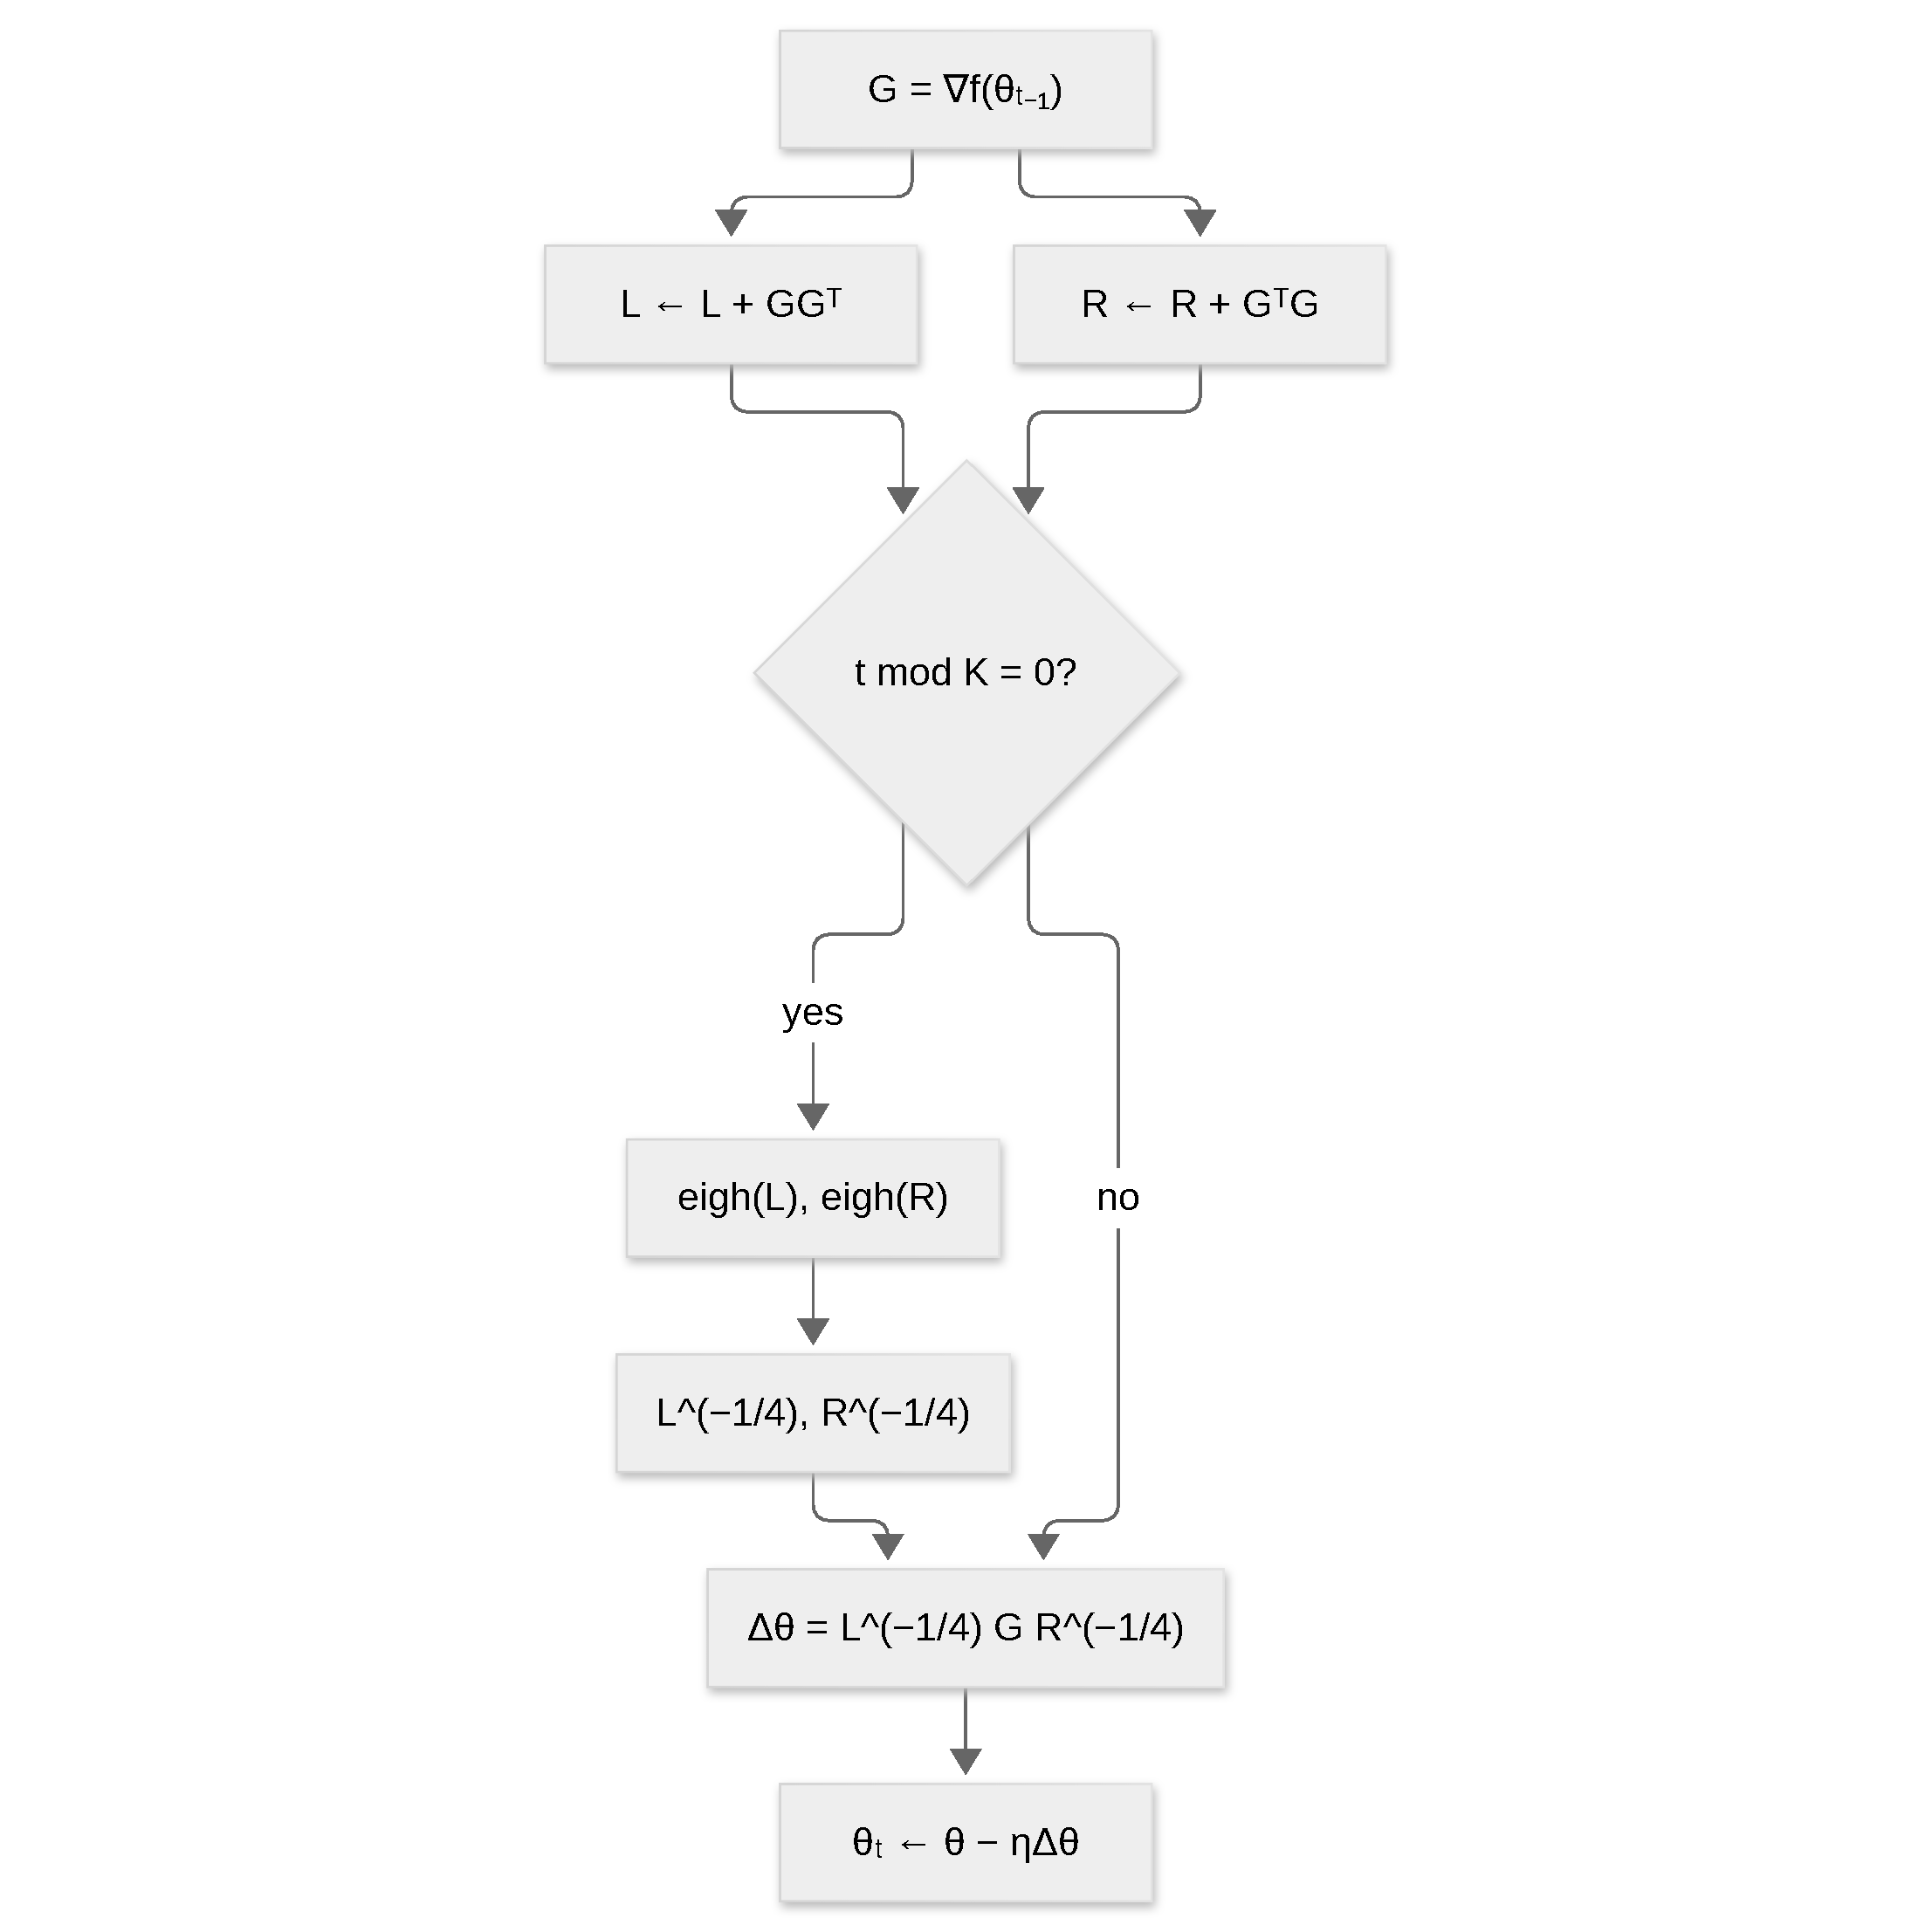
\includegraphics{figures/optimizers/shampoo.pdf}}
\caption{Step flow of Shampoo: Kronecker-factored Gram matrices, periodic eigendecomposition, and fourth-root preconditioning of the gradient.}
\label{fig:opt-shampoo}
\end{figure}
Shampoo is a \textbf{structured second-order method} that computes matrix preconditioners from Kronecker-structured outer-product statistics. For a 2D parameter matrix $W \in \mathbb{R}^{m \times n}$:
\begin{align}
L_t &= L_{t-1} + G_t G_t^\top \quad\text{(left/row Gram matrix, $m \times m$)} \\
R_t &= R_{t-1} + G_t^\top G_t \quad\text{(right/column Gram matrix, $n \times n$)} \\
L_t^{-1/4} &= Q_L (\Lambda_L)^{-1/4} Q_L^\top \quad\text{(via eigendecomposition)} \\
R_t^{-1/4} &= Q_R (\Lambda_R)^{-1/4} Q_R^\top \\
\Delta W_t &= L_t^{-1/4} G_t R_t^{-1/4} \quad\text{(preconditioned gradient)}
\end{align}
Shampoo approximates the full-matrix Adagrad preconditioner $H^{-1/2}$ (where $H$ is the Hessian) using Kronecker-factored structure. Instead of storing a $(mn) \times (mn)$ preconditioner, Shampoo maintains two smaller matrices ($m \times m$ and $n \times n$), capturing cross-parameter correlations within and across groups. Eigendecompositions are performed periodically (e.g., every $K=10$ steps) to amortize cost.

\begin{algorithm}[H]
\caption{Shampoo (Matrix Preconditioning via Kronecker Products)}
\label{alg:shampoo}
\begin{algorithmic}[1]
\Require Initial parameters $\theta_0$, learning rate $\eta$, eigendecomposition interval $K$
\Ensure Updated parameters $\theta_T$
\State Initialize: $L \gets \epsilon I_m$, $R \gets \epsilon I_n$ (left and right Gram matrices)
\For{$t = 1, 2, \ldots, T$}
    \State $G \gets \nabla f(\theta_{t-1})$ \Comment{Gradient}
    \State Update Gram matrices: $L \gets L + G G^\top$, $R \gets R + G^\top G$
    \If{$t \mod K == 0$}
        \State $Q_L, \Lambda_L \gets \text{eigh}(L)$ \Comment{Eigendecomposition of $L$}
        \State $Q_R, \Lambda_R \gets \text{eigh}(R)$ \Comment{Eigendecomposition of $R$}
        \State $L^{-1/4} \gets Q_L (\Lambda_L + \epsilon)^{-1/4} Q_L^\top$
        \State $R^{-1/4} \gets Q_R (\Lambda_R + \epsilon)^{-1/4} Q_R^\top$
    \EndIf
    \State $\Delta \theta \gets L^{-1/4} G R^{-1/4}$ \Comment{Preconditioned gradient}
    \State $\theta_t \gets \theta_{t-1} - \eta \cdot \Delta \theta$
\EndFor
\Return $\theta_T$
\end{algorithmic}
\end{algorithm}

\paragraph{Cons.}
\begin{itemize}[leftmargin=*]
\item Periodic $O(m^3 + n^3)$ eigendecompositions and higher per-step compute.
\item Assumes 2D parameter structure; embeddings and biases need separate handling.
\end{itemize}

\paragraph{Pros.}
\begin{itemize}[leftmargin=*]
\item Kronecker-factored second-order preconditioning without a dense $(mn) \times (mn)$ matrix.
\item Proven effective at production scale and well suited to high-rank transformer matrices, with improved conditioning and accelerated convergence.
\end{itemize}

\paragraph{SOAP (Shampoo with Adam in eigenbasis).}
\begin{figure}[H]
\centering
\fitfigure{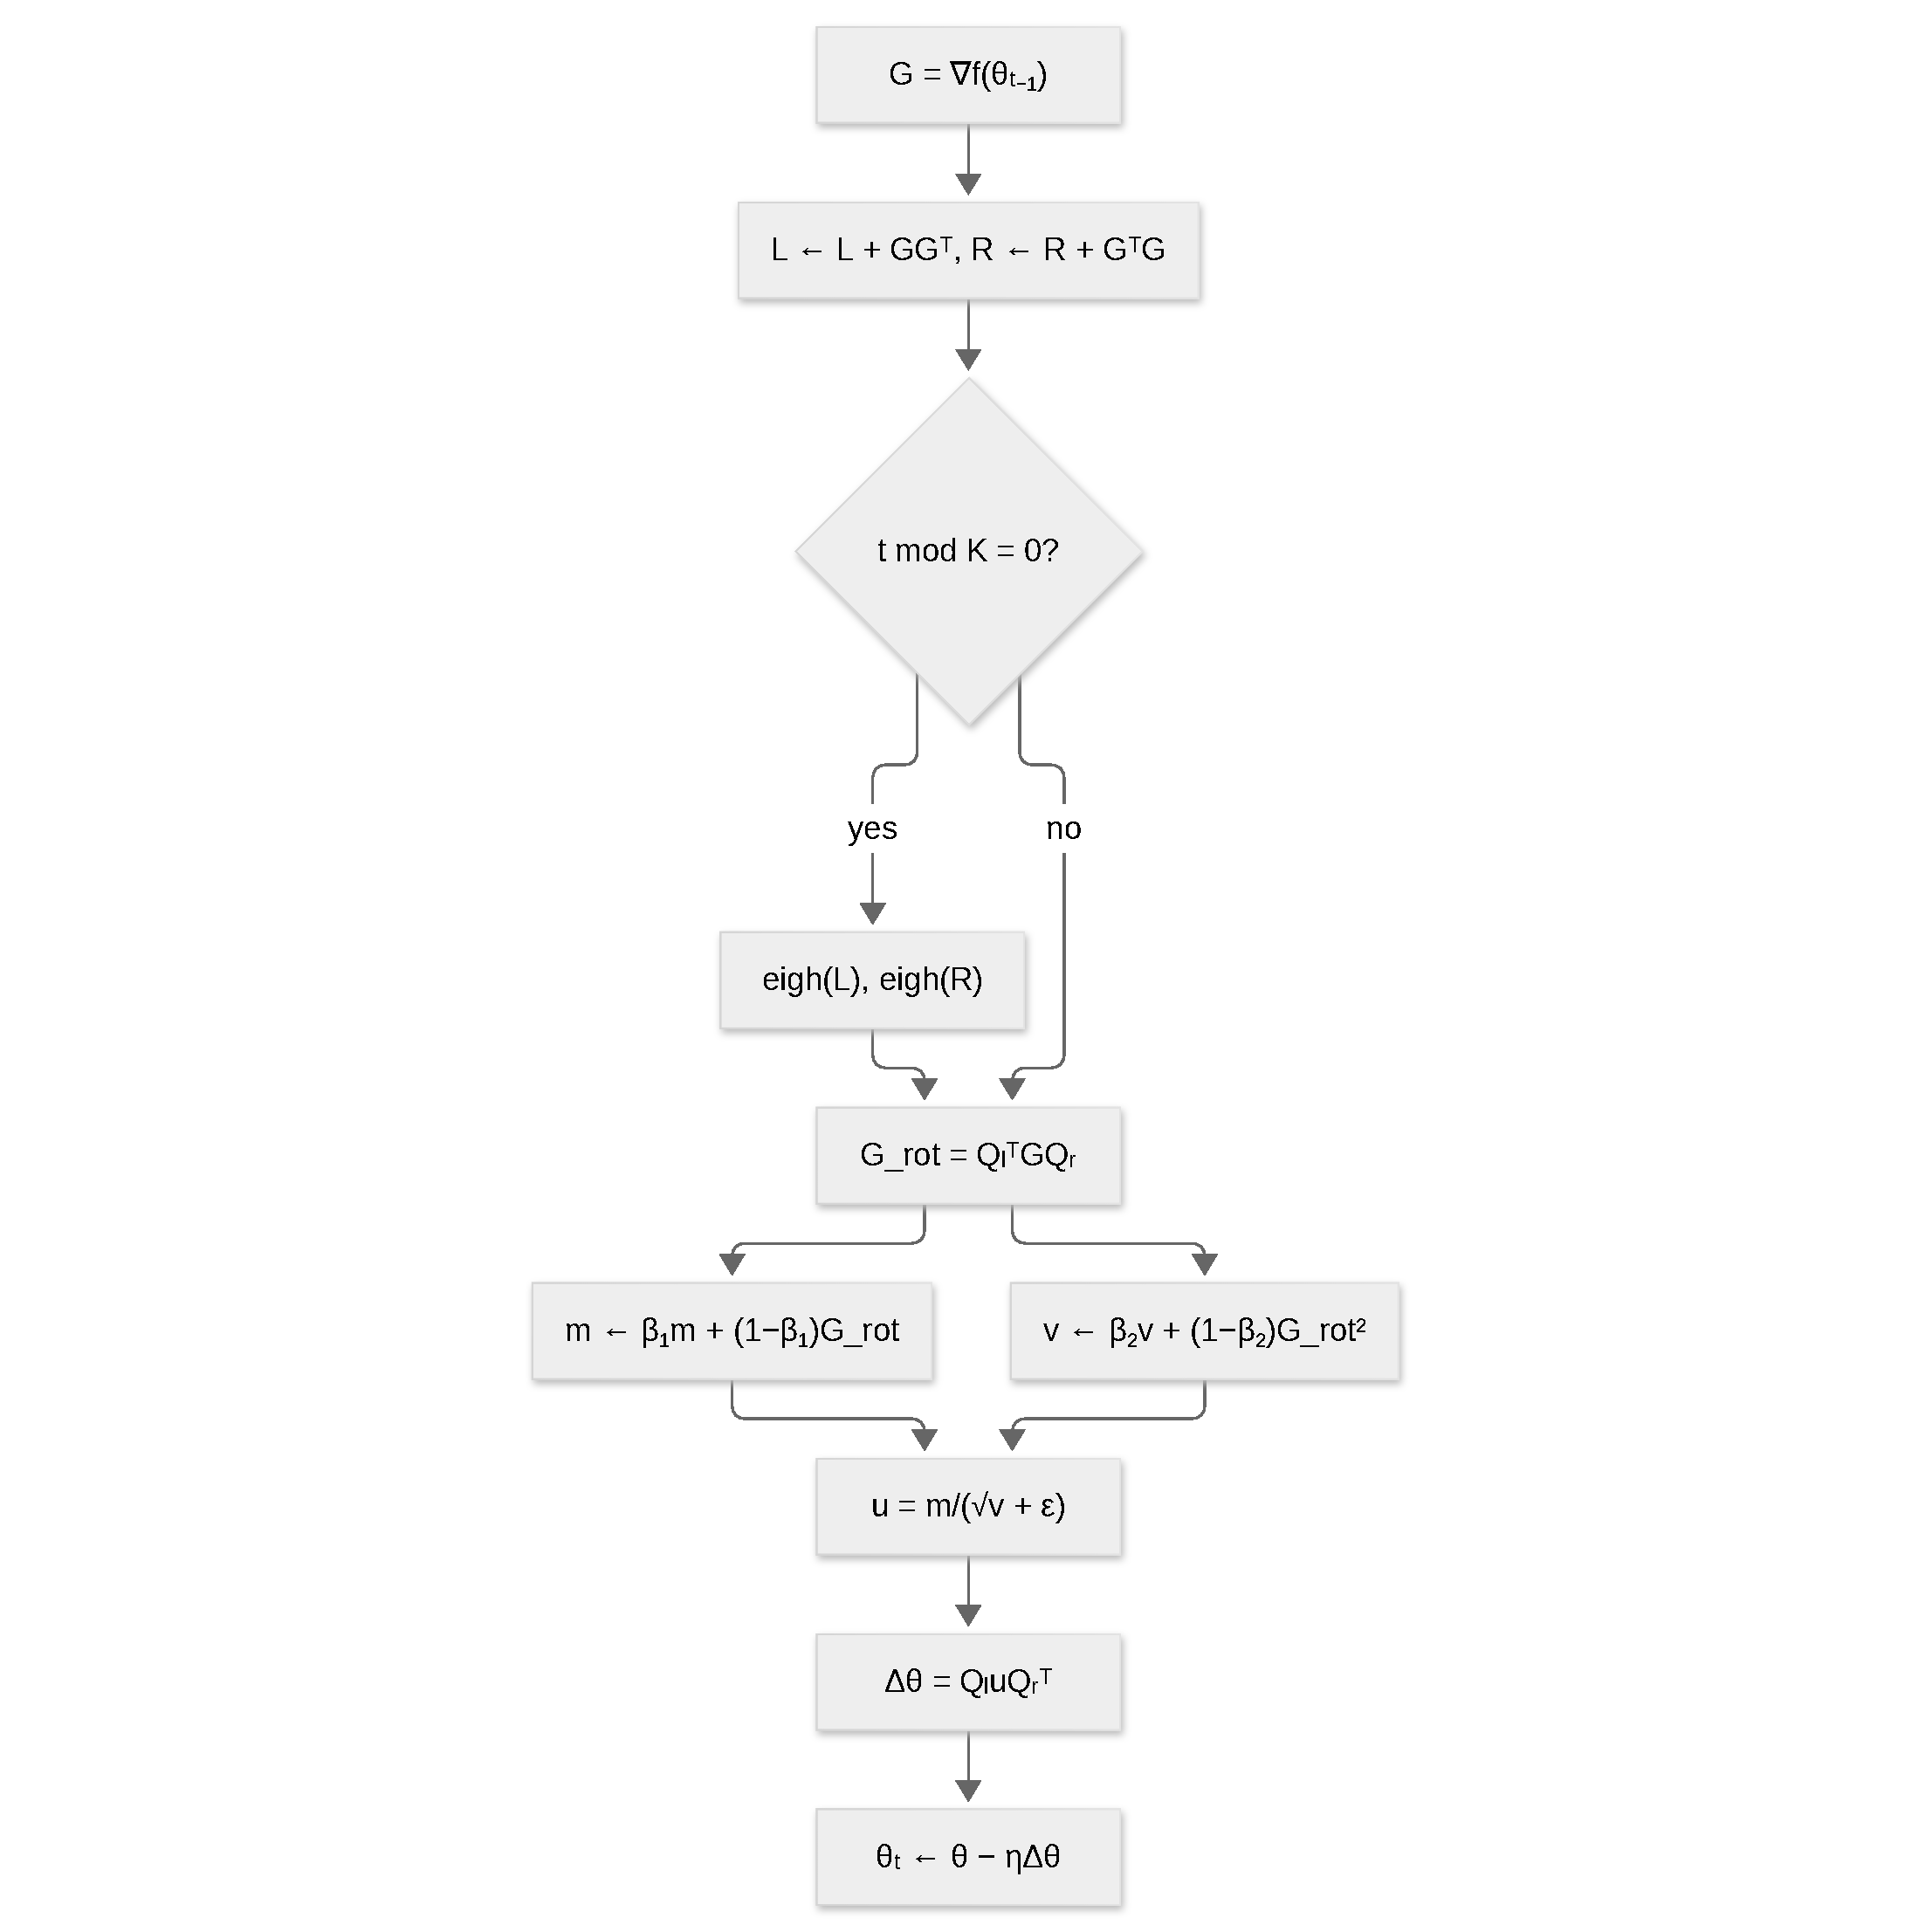
\includegraphics{figures/optimizers/soap.pdf}}
\caption{Step flow of SOAP: Adam moments tracked in the Shampoo eigenbasis and rotated back to parameter space.}
\label{fig:opt-soap}
\end{figure}
SOAP is a simplified variant of Shampoo that decouples preconditioning from momentum tracking. Instead of complex matrix algebra on preconditioned gradients, SOAP runs standard Adam in the eigenbasis of Shampoo's preconditioners:
\begin{align}
L_t &= L_{t-1} + G_t G_t^\top, \quad R_t = R_{t-1} + G_t^\top G_t \quad\text{(Gram accumulation)} \\
Q_L, \Lambda_L &= \text{eigh}(L_t), \quad Q_R, \Lambda_R = \text{eigh}(R_t) \quad\text{(periodic eigendecomposition)} \\
G_t^{\text{rot}} &= Q_L^\top G_t Q_R \quad\text{(rotate gradient into eigenbasis)} \\
m_t^{\text{rot}} &= \beta_1 m_{t-1}^{\text{rot}} + (1-\beta_1) G_t^{\text{rot}} \\
v_t^{\text{rot}} &= \beta_2 v_{t-1}^{\text{rot}} + (1-\beta_2)(G_t^{\text{rot}})^2 \quad\text{(Adam in rotated space)} \\
U_t^{\text{rot}} &= \frac{m_t^{\text{rot}}}{\sqrt{v_t^{\text{rot}}}+\epsilon}, \quad U_t = Q_L U_t^{\text{rot}} Q_R^\top \quad\text{(rotate back)}
\end{align}
The key insight: all momentum tracking occurs in the well-conditioned eigenbasis, simplifying numerical stability and theoretical analysis.

\begin{algorithm}[H]
\caption{SOAP (Shampoo with Adam in Eigenbasis)}
\label{alg:soap}
\begin{algorithmic}[1]
\Require Initial parameters $\theta_0$, learning rate $\eta$, $\beta_1, \beta_2$, eigendecomposition interval $K$
\Ensure Updated parameters $\theta_T$
\State Initialize: $L \gets \epsilon I_m$, $R \gets \epsilon I_n$, $m \gets 0$, $v \gets 0$
\For{$t = 1, 2, \ldots, T$}
    \State $G \gets \nabla f(\theta_{t-1})$ \Comment{Gradient}
    \State Update Gram: $L \gets L + G G^\top$, $R \gets R + G^\top G$
    \If{$t \mod K == 0$}
        \State $Q_L, \Lambda_L \gets \text{eigh}(L)$, $Q_R, \Lambda_R \gets \text{eigh}(R)$
    \EndIf
    \State $G^{\text{rot}} \gets Q_L^\top G Q_R$ \Comment{Rotate gradient into eigenbasis}
    \State $m \gets \beta_1 m + (1-\beta_1) G^{\text{rot}}$ \Comment{Exponential moving average (bias-correct outside)}
    \State $v \gets \beta_2 v + (1-\beta_2) (G^{\text{rot}})^2$ \Comment{Second moment (bias-correct outside)}
    \State $u \gets m / (\sqrt{v} + \epsilon)$ \Comment{Adaptive step in eigenbasis}
    \State $\Delta \theta \gets Q_L u Q_R^\top$ \Comment{Rotate back to parameter space}
    \State $\theta_t \gets \theta_{t-1} - \eta \cdot \Delta \theta$
\EndFor
\Return $\theta_T$
\end{algorithmic}
\end{algorithm}

\paragraph{Cons.}
\begin{itemize}[leftmargin=*]
\item Inherits Shampoo's periodic eigendecomposition cost.
\item Rotation and inverse rotation add matrix multiplications per step.
\end{itemize}

\paragraph{Pros.}
\begin{itemize}[leftmargin=*]
\item Combines Shampoo's explicit curvature structure with Adam's proven momentum mechanics.
\item Often cleaner and more stable than full Shampoo, with eigendecompositions amortized every $K$ steps.
\end{itemize}

\paragraph{Lion (EvoLved Sign Momentum).}
\begin{figure}[H]
\centering
\fitfigure{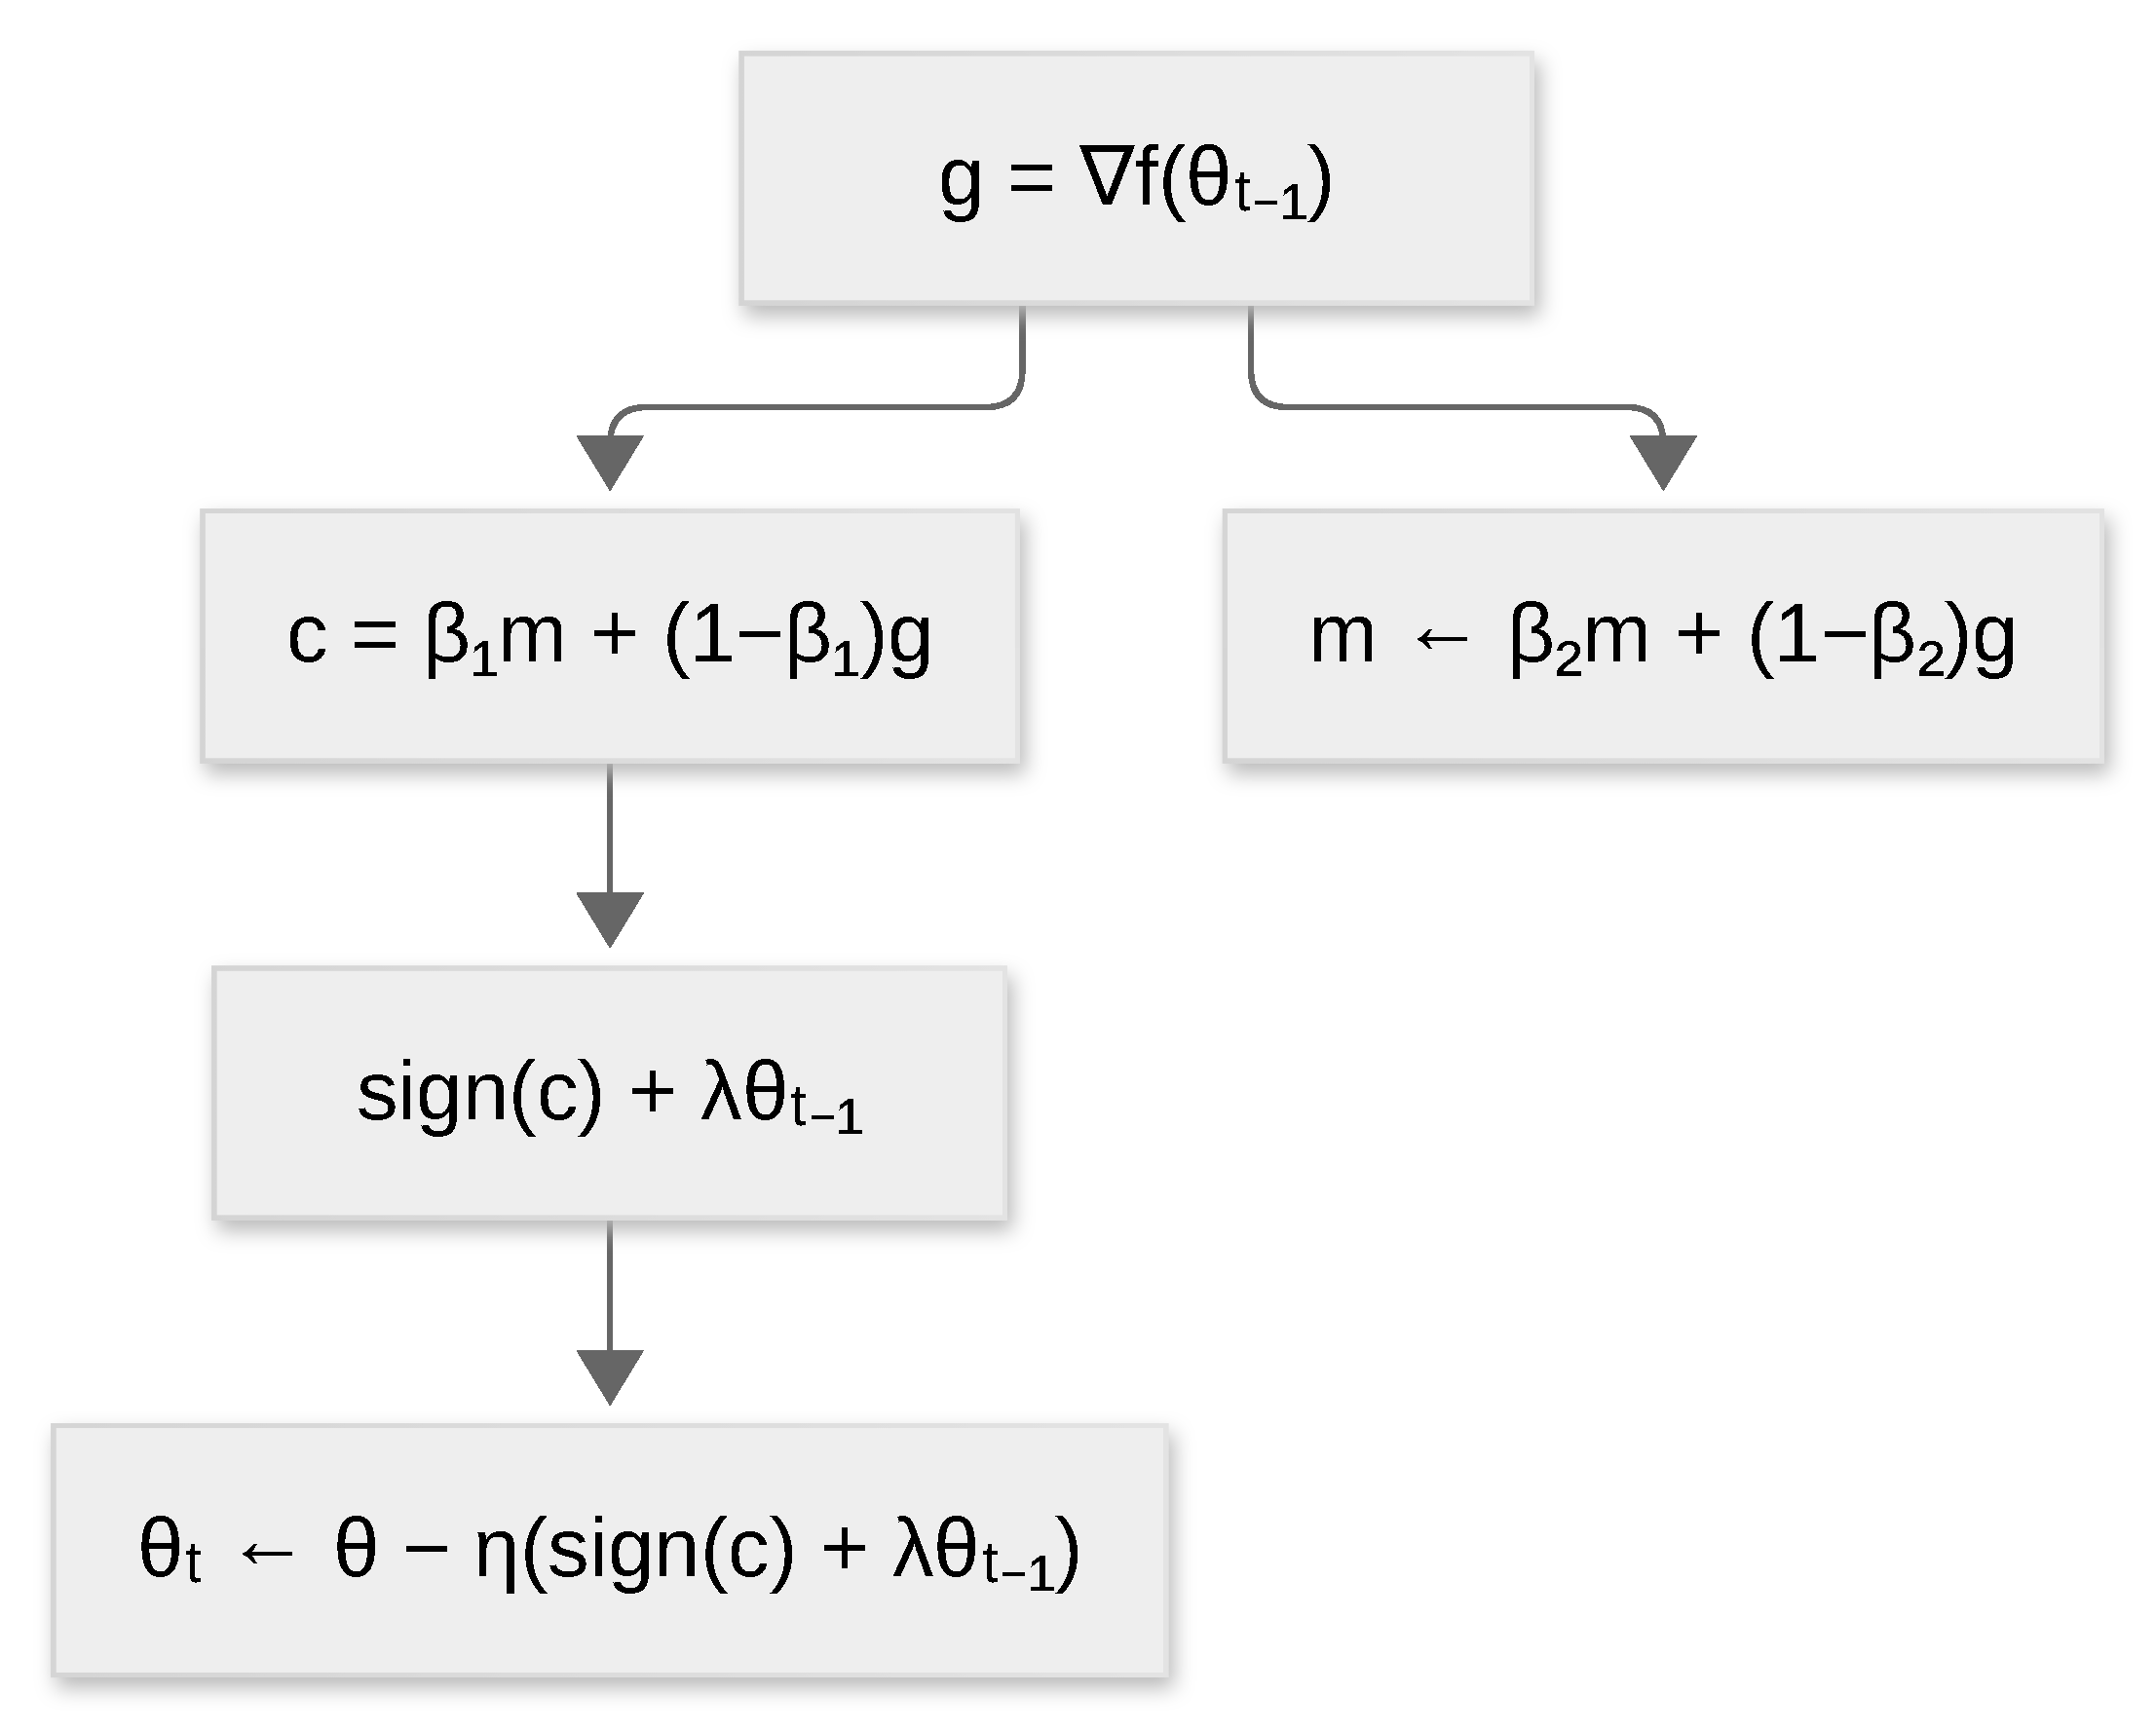
\includegraphics{figures/optimizers/lion.pdf}}
\caption{Step flow of Lion: sign-of-momentum update with decoupled momentum accumulation and weight decay.}
\label{fig:opt-lion}
\end{figure}
Lion achieves \textbf{minimal memory overhead} by using sign-based updates instead of full adaptive scaling:
\begin{align}
c_t &= \beta_1 m_t + (1-\beta_1) g_t \quad\text{(momentum input)} \\
\theta_{t+1} &= \theta_t - \eta \left(\text{sign}(c_t) + \lambda\theta_t\right) \quad\text{(sign operator update)} \\
m_{t+1} &= \beta_2 m_t + (1-\beta_2) g_t \quad\text{(momentum accumulation)}
\end{align}
All element-wise scaling operations are replaced with \texttt{sign()}, which outputs $\{-1, 0, +1\}$. This dramatically reduces memory compared to Adam-like methods: Lion stores only the momentum buffer, no second moment variance.

\begin{algorithm}[H]
\caption{Lion (EvoLved Sign Momentum)}
\label{alg:lion}
\begin{algorithmic}[1]
\Require Initial parameters $\theta_0$, learning rate $\eta$, $\beta_1, \beta_2$, weight decay $\lambda$
\Ensure Updated parameters $\theta_T$
\State Initialize: $m \gets 0$ (momentum buffer)
\For{$t = 1, 2, \ldots, T$}
    \State $g \gets \nabla f(\theta_{t-1})$ \Comment{Gradient}
    \State $c \gets \beta_1 m + (1-\beta_1) g$ \Comment{Momentum input}
    \State $\theta_t \gets \theta_{t-1} - \eta (\text{sign}(c) + \lambda \theta_{t-1})$ \Comment{Sign-based update with weight decay}
    \State $m \gets \beta_2 m + (1-\beta_2) g$ \Comment{Momentum accumulation (decoupled)}
\EndFor
\Return $\theta_T$
\end{algorithmic}
\end{algorithm}

\paragraph{Cons.}
\begin{itemize}[leftmargin=*]
\item Sign-based updates sacrifice the element-wise learning-rate adaptation that makes Adam effective.
\item Can be less robust than Adam-family methods on tasks that need adaptive scaling.
\end{itemize}

\paragraph{Pros.}
\begin{itemize}[leftmargin=*]
\item Stores only the momentum buffer, with no second moment variance.
\item High-throughput, low-memory option for large-batch regimes where activation memory dominates.
\end{itemize}

\paragraph{Sophia (Second-Order Hessian Information with Optimized Approximation).}
\begin{figure}[H]
\centering
\fitfigure{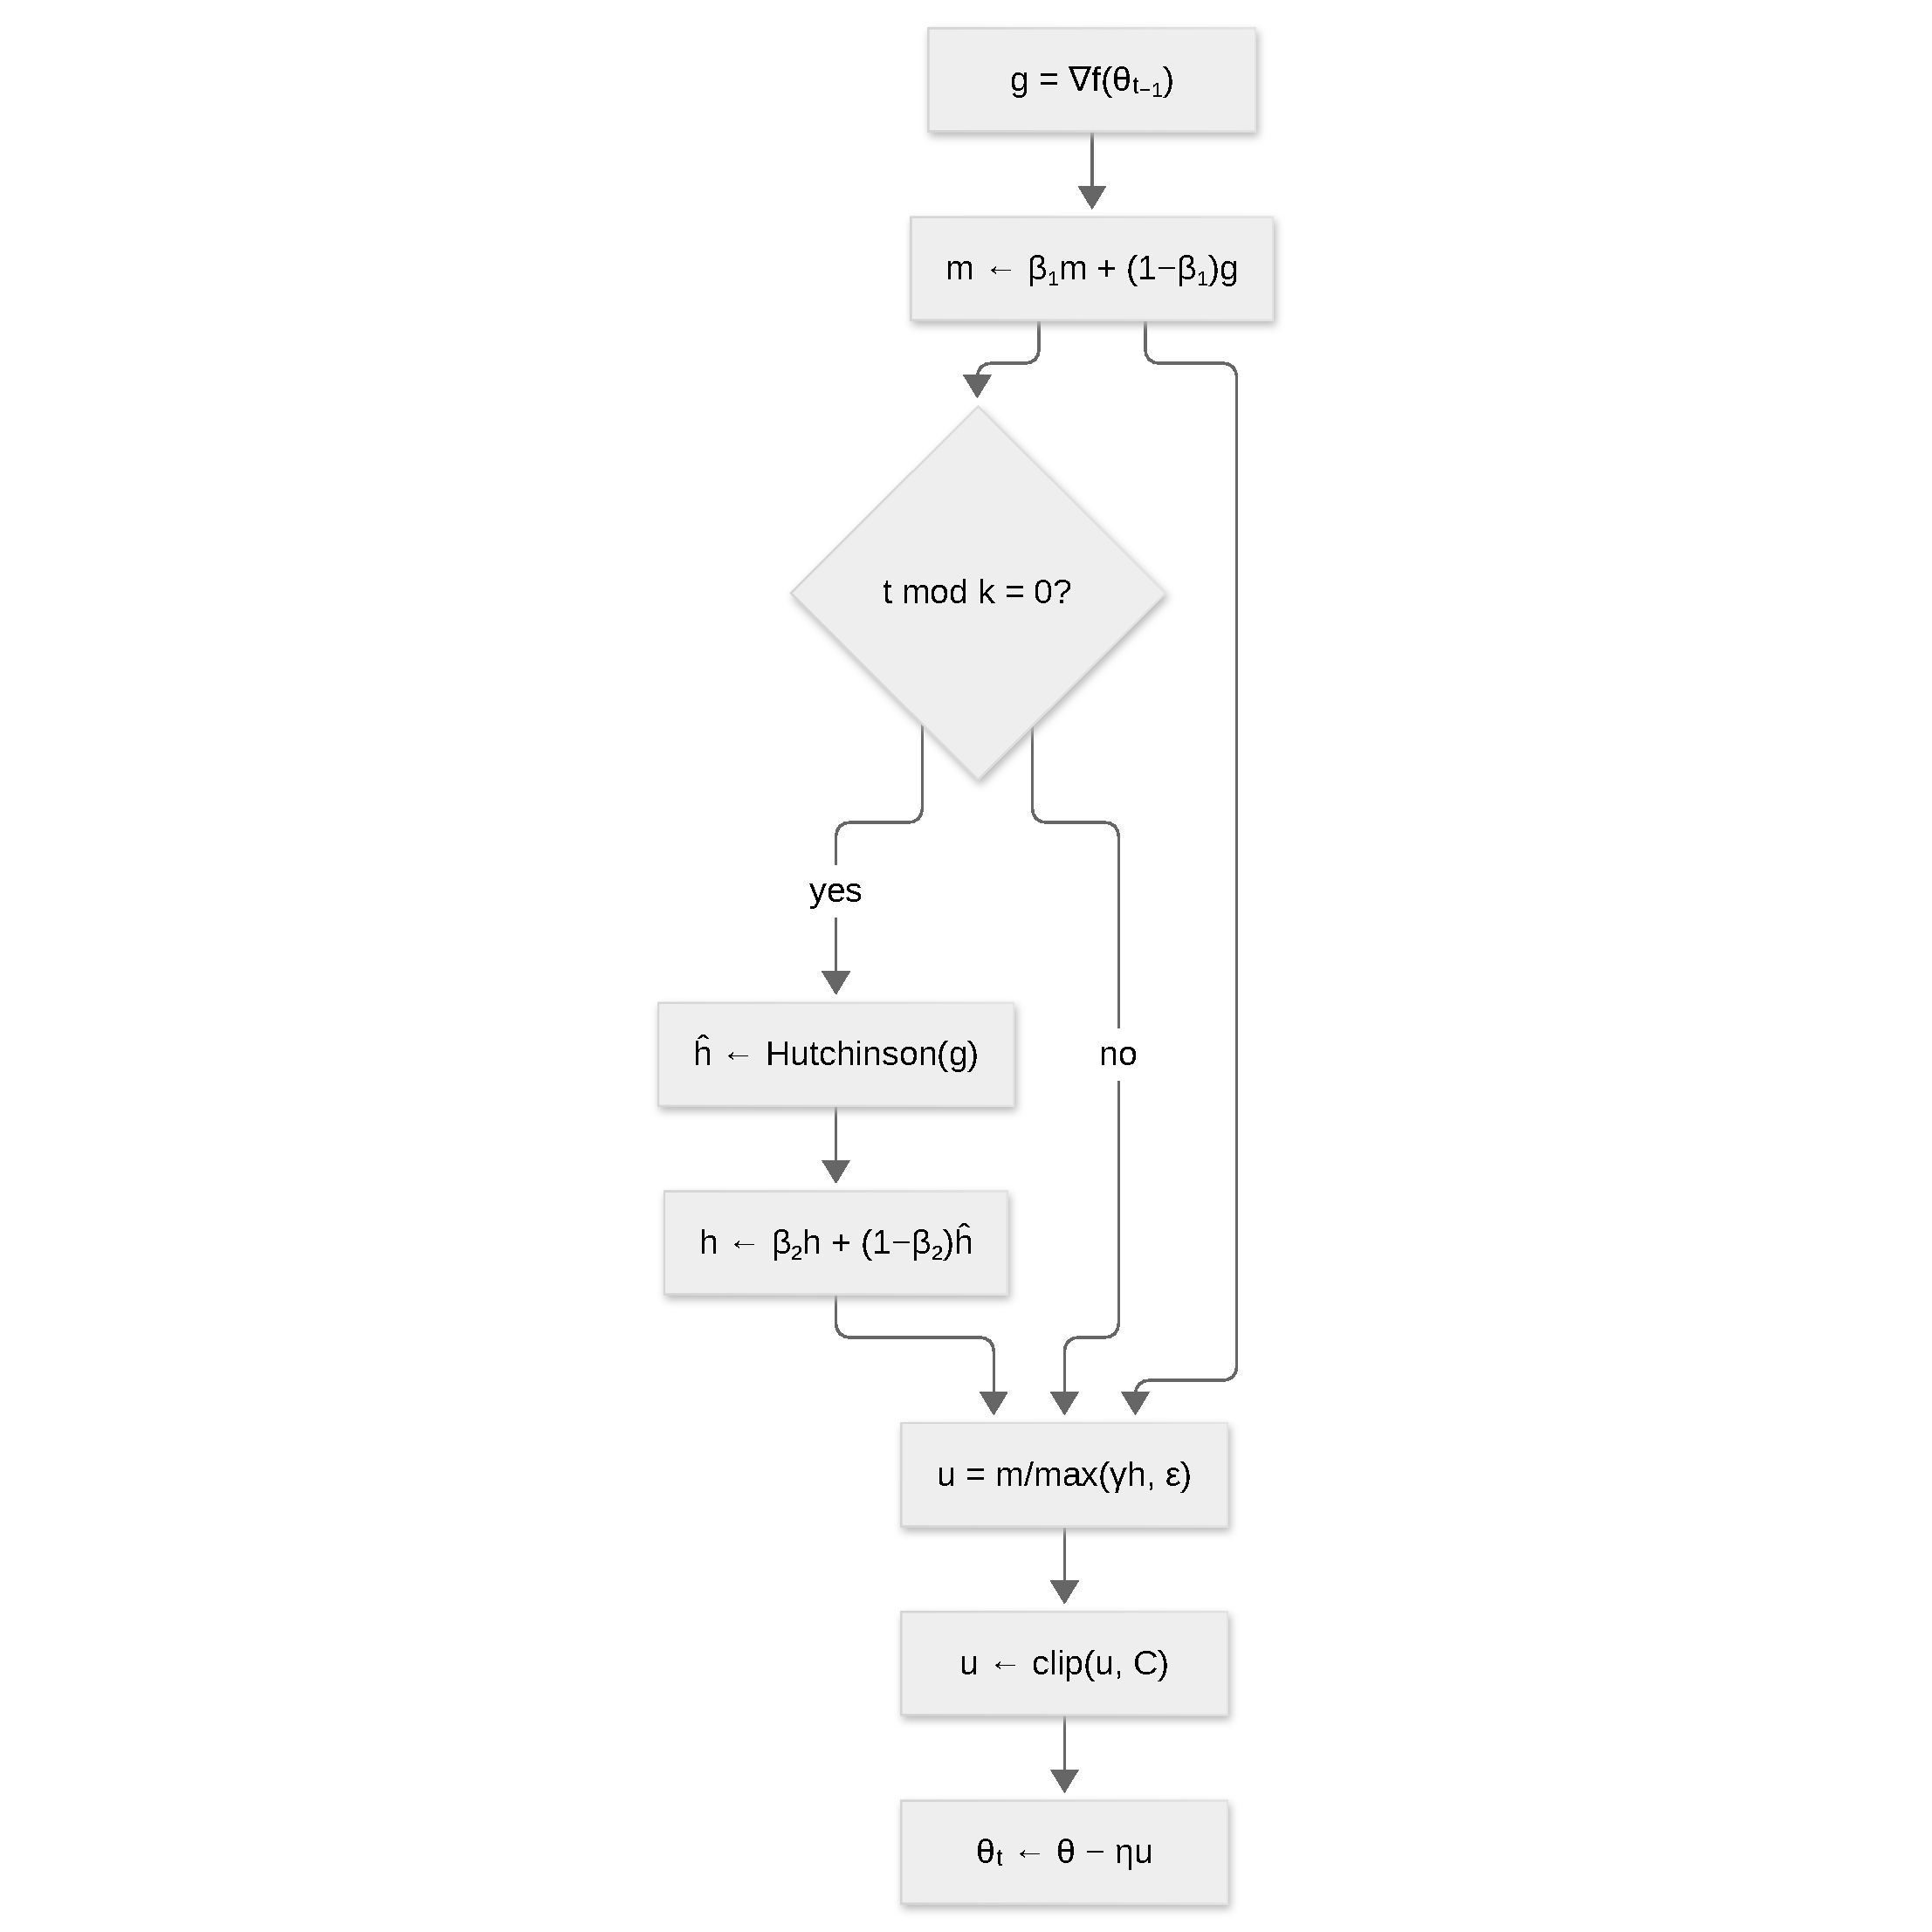
\includegraphics{figures/optimizers/sophia.pdf}}
\caption{Step flow of Sophia: diagonal Hutchinson Hessian estimate with clipped, curvature-aware element-wise steps.}
\label{fig:opt-sophia}
\end{figure}
Sophia uses \textbf{diagonal Hessian estimates} for curvature-aware scaling without the memory and compute cost of dense second-order methods.
\begin{align}
m_t &= \beta_1 m_{t-1} + (1-\beta_1) g_t \quad\text{(first moment)} \\
h_t &= \beta_2 h_{t-(k-1)} + (1-\beta_2) \hat{h}_t \quad\text{(diagonal Hessian, updated every $k$ steps)} \\
\text{clip}(x, C) &= \min(\max(x, -C), C) \quad\text{(element-wise clipping)} \\
\theta_{t+1} &= \theta_t - \eta \cdot \text{clip}\left(\frac{m_t}{\max(\gamma h_t, \epsilon)}, 1\right)
\end{align}
where $\hat{h}_t$ is a diagonal estimate (e.g., Hutchinson-trace estimator) and $\gamma$ is a scaling factor. The diagonal Hessian $h_t$ captures local curvature, allowing the optimizer to take smaller steps in sharp directions and larger steps in flat directions. The clipping operation $\text{clip}(\cdot, 1)$ prevents adaptive steps from exploding.

\begin{algorithm}[H]
\caption{Sophia (Diagonal Hessian with Clipped Updates)}
\label{alg:sophia}
\begin{algorithmic}[1]
\Require Initial parameters $\theta_0$, learning rate $\eta$, $\beta_1, \beta_2$, Hessian update freq $k$, clip threshold $C$
\Ensure Updated parameters $\theta_T$
\State Initialize: $m \gets 0$, $h \gets \epsilon$ (diagonal Hessian estimate)
\For{$t = 1, 2, \ldots, T$}
    \State $g \gets \nabla f(\theta_{t-1})$
    \State $m \gets \beta_1 m + (1-\beta_1) g$ \Comment{First moment (bias-correct outside)}
    \If{$t \mod k == 0$}
        \State $\hat{h} \gets \text{HutchinsonEstimate}(g)$ \Comment{Diagonal Hessian via Hutchinson}
        \State $h \gets \beta_2 h + (1-\beta_2) \hat{h}$ \Comment{Update Hessian estimate}
    \EndIf
    \State $u \gets \frac{m}{\max(\gamma h, \epsilon)}$ \Comment{Adaptive step (element-wise)}
    \State $u \gets \text{clip}(u, C)$ \Comment{Element-wise clipping to $[-C, C]$}
    \State $\theta_t \gets \theta_{t-1} - \eta \cdot u$
\EndFor
\Return $\theta_T$
\end{algorithmic}
\end{algorithm}

\paragraph{Cons.}
\begin{itemize}[leftmargin=*]
\item Hutchinson estimates add periodic compute and noise to the curvature signal.
\item The Hessian estimate can become stale between refreshes.
\end{itemize}

\paragraph{Pros.}
\begin{itemize}[leftmargin=*]
\item Curvature-aware scaling without the $O(n^2)$ or $O(n^3)$ cost of full second-order methods.
\item Clipped steps prevent explosions and work particularly well in second-pass fine-tuning.
\end{itemize}

\paragraph{Muon (Newton-Schulz Orthogonalization).}
\begin{figure}[H]
\centering
\fitfigure{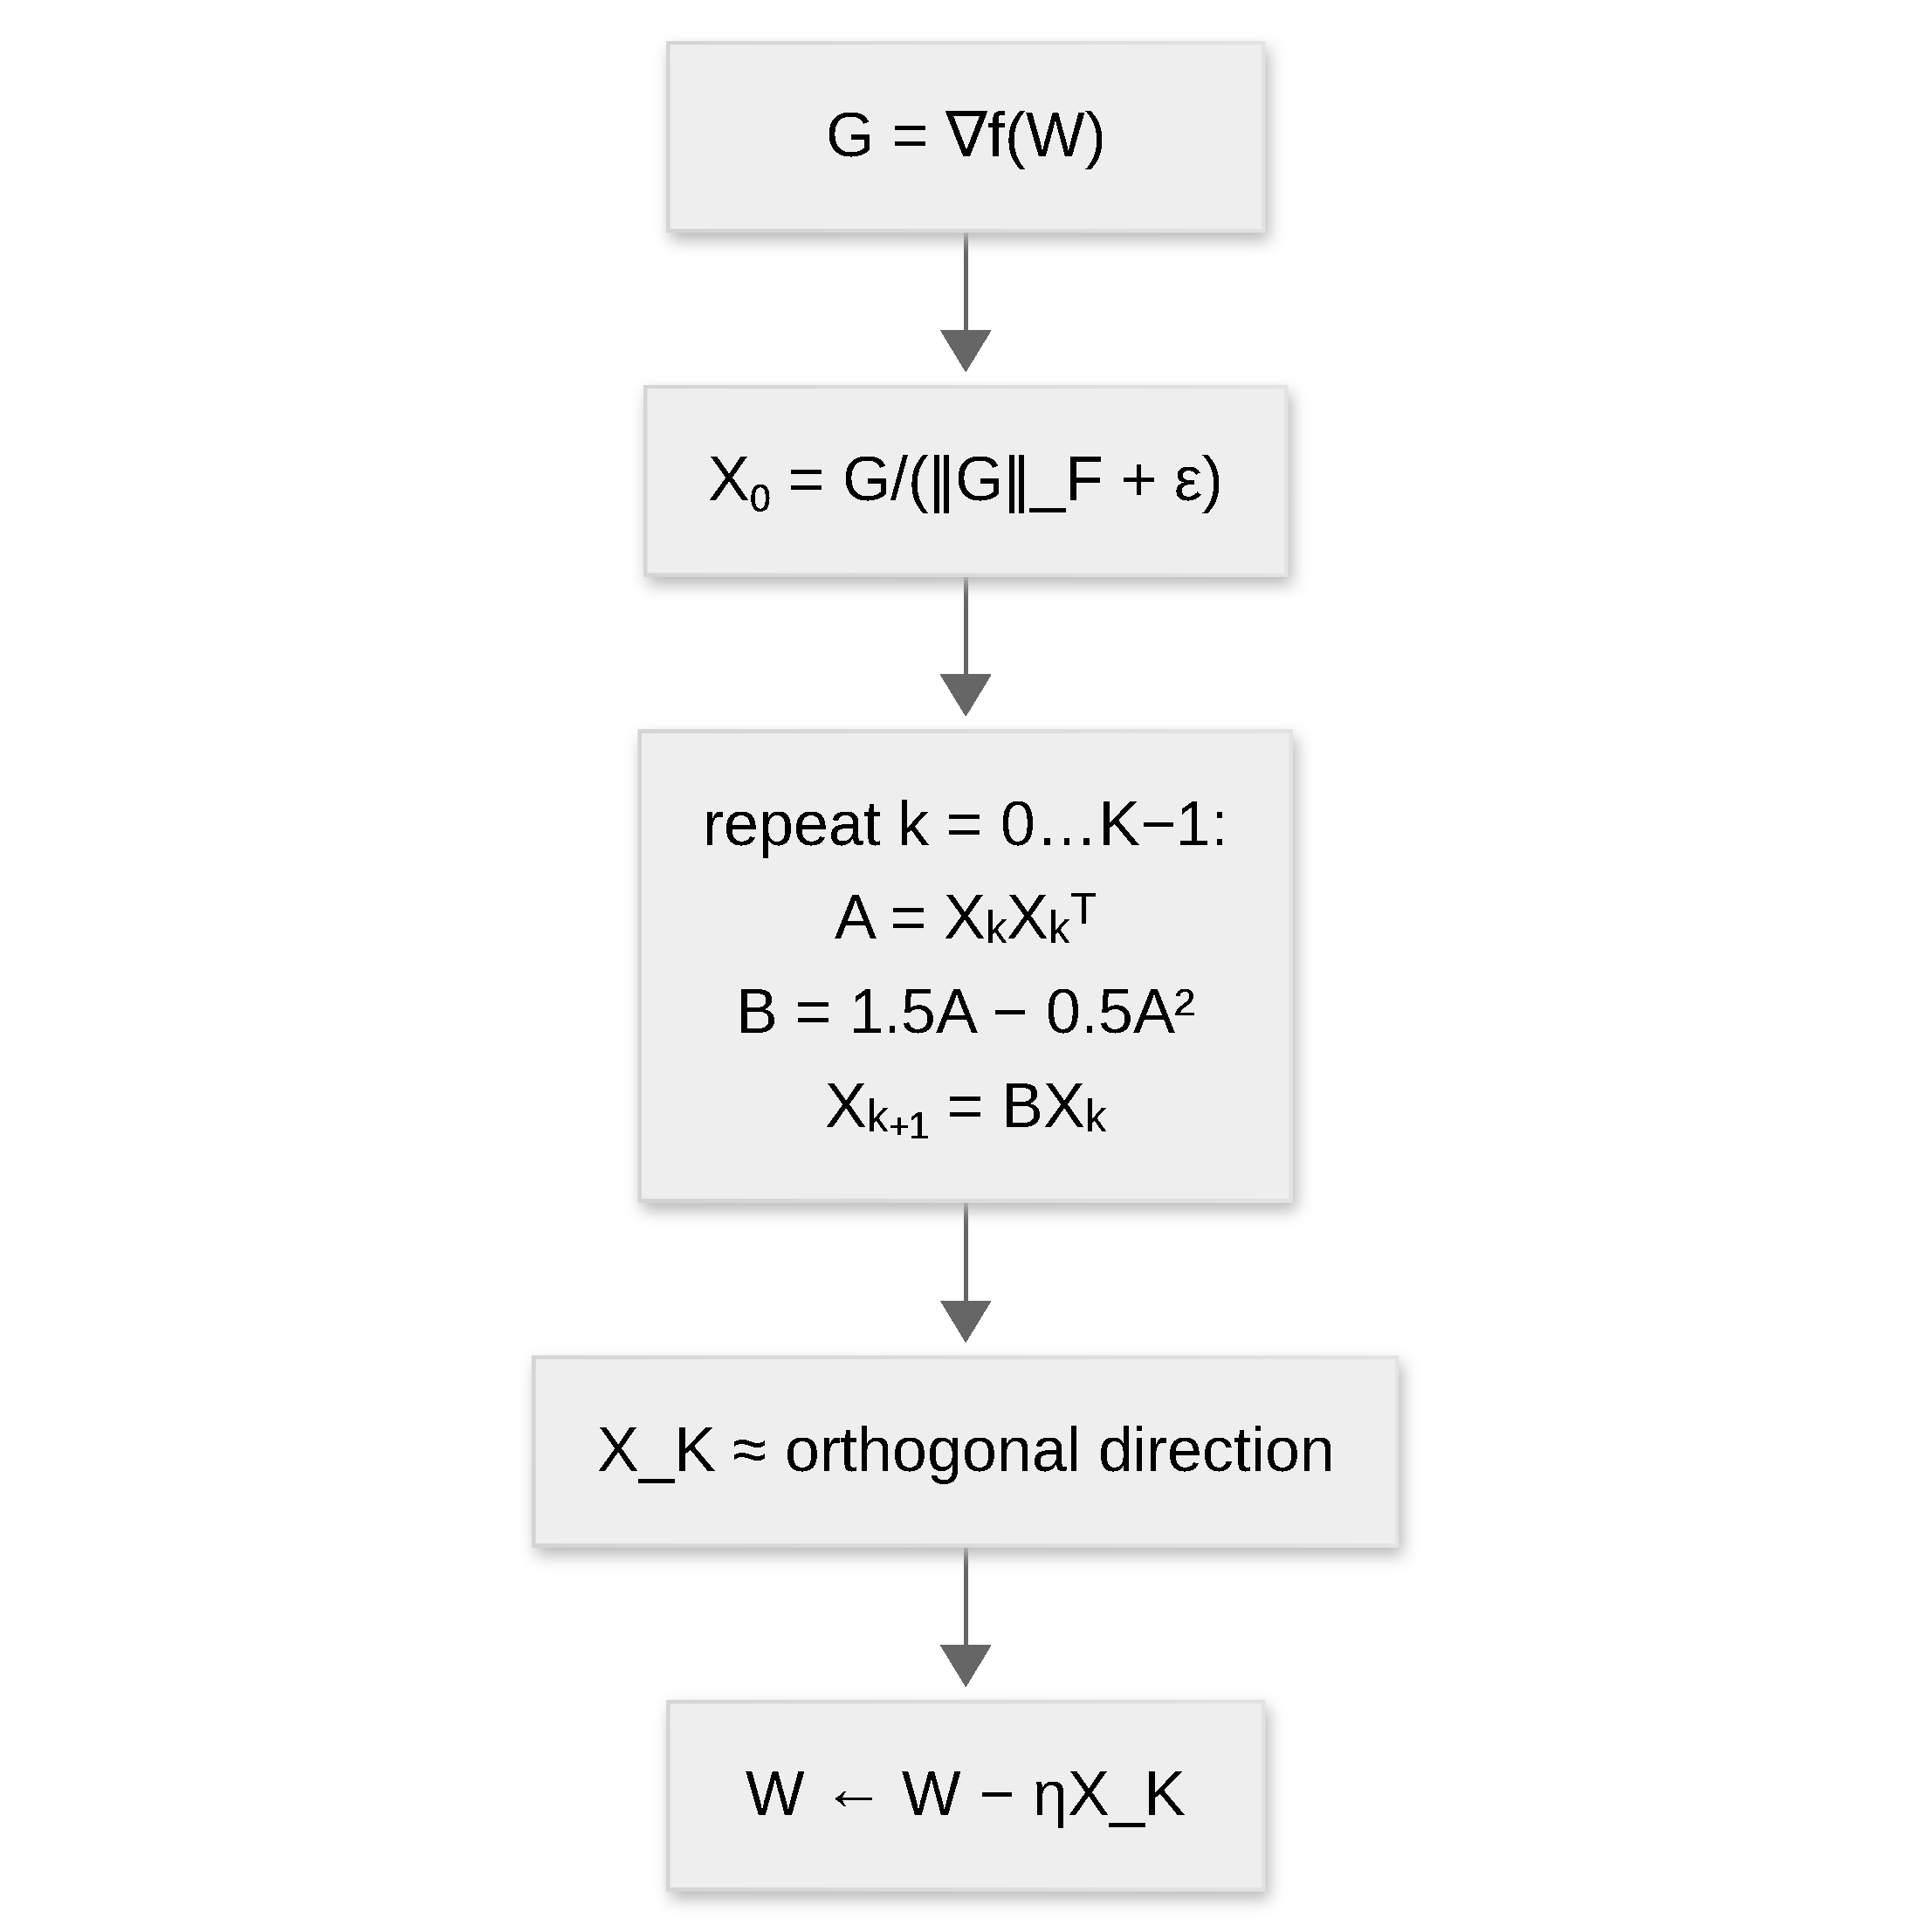
\includegraphics{figures/optimizers/muon.pdf}}
\caption{Step flow of Muon: Frobenius normalization followed by Newton-Schulz iterations that orthogonalize the update direction.}
\label{fig:opt-muon}
\end{figure}
Muon is an \textbf{orthogonality-oriented optimizer} that reshapes update geometry using Newton-Schulz polynomial iterations for orthogonalization. For a 2D parameter matrix $W$ with gradient $G_t$:
\begin{align}
X_0 &= \frac{G_t}{\|G_t\|_F + \epsilon} \quad\text{(normalized gradient)} \\
A_k &= X_k X_k^\top \quad\text{(Gramian)} \\
B_k &= b A_k + c A_k^2 \quad\text{(polynomial step, coefficients $b, c$ from Newton-Schulz)} \\
X_{k+1} &= a X_k + B_k X_k \quad\text{(iteration $k=0,1,\ldots,4$)} \\
W_{t+1} &= W_t - \eta X_K \quad\text{(update with orthogonalized direction)}
\end{align}
Muon performs 5 Newton-Schulz iterations to produce an approximately orthogonal direction, ensuring updates respect geometric constraints. The rationale: orthogonal updates preserve norms during training, avoiding the norm creep observed in momentum-based methods.

Following the hybrid recipe of \citet{shen_convergence_2025}, the orthogonalized update is reserved for hidden-layer weight matrices ($\mathtt{attention}$, $\mathtt{ffn}$ and other hidden-block groups). Embedding tables, learned positional encodings, output heads and every non-matrix parameter (biases, normalization scales, convolution kernels) are trained with decoupled AdamW instead of being skipped, using the group-level learning rate, weight decay, $\beta_1, \beta_2$ and $\epsilon$ settings exposed by the per-group configuration.

\begin{algorithm}[H]
\caption{Muon (Newton-Schulz Orthogonalization)}
\label{alg:muon}
\begin{algorithmic}[1]
\Require Initial parameters $\theta$, learning rate $\eta$, Newton-Schulz iters $K$
\Ensure Updated parameters $\theta_T$
\For{each parameter $P$}
    \If{$P$ is a hidden-layer 2D matrix $W$}
        \State $G \gets \nabla f(W)$ \Comment{Gradient}
        \State $X_0 \gets \frac{G}{\|G\|_F + \epsilon}$ \Comment{Normalize gradient by Frobenius norm}
        \For{$k = 0, 1, \ldots, K-1$}
            \State $A_k \gets X_k X_k^\top$ \Comment{Gramian (cost: $O(mn^2)$ or $O(m^2n)$ for tall/wide)}
            \State $B_k \gets (3/2) A_k - (1/2) A_k^2$ \Comment{Newton-Schulz coefficients}
            \State $X_{k+1} \gets B_k X_k$ \Comment{Polynomial step}
        \EndFor
        \State $W \gets W - \eta X_K$ \Comment{Update with orthogonalized direction}
    \Else
        \State $P \gets \operatorname{AdamW}(P, \nabla f(P); \eta, \beta_1, \beta_2, \epsilon, \lambda)$ \Comment{Hybrid fallback: embeddings, pos, heads, non-matrices}
    \EndIf
\EndFor
\Return $\theta_T$
\end{algorithmic}
\end{algorithm}

\paragraph{Cons.}
\begin{itemize}[leftmargin=*]
\item Several matrix multiplications per Newton-Schulz iteration; efficient custom kernels are required.
\item The orthogonalized construction is defined only for 2D matrices; the remaining parameter classes depend on the AdamW fallback and its per-group learning-rate calibration.
\end{itemize}

\paragraph{Pros.}
\begin{itemize}[leftmargin=*]
\item Orthogonalized updates preserve norms and avoid the norm creep of momentum-based methods.
\item Promising results on large-scale training with fundamentally better-conditioned update geometry.
\end{itemize}

\paragraph{Turbo-Muon (AOL-Preconditioned Orthogonalization).}
\begin{figure}[H]
\centering
\fitfigure{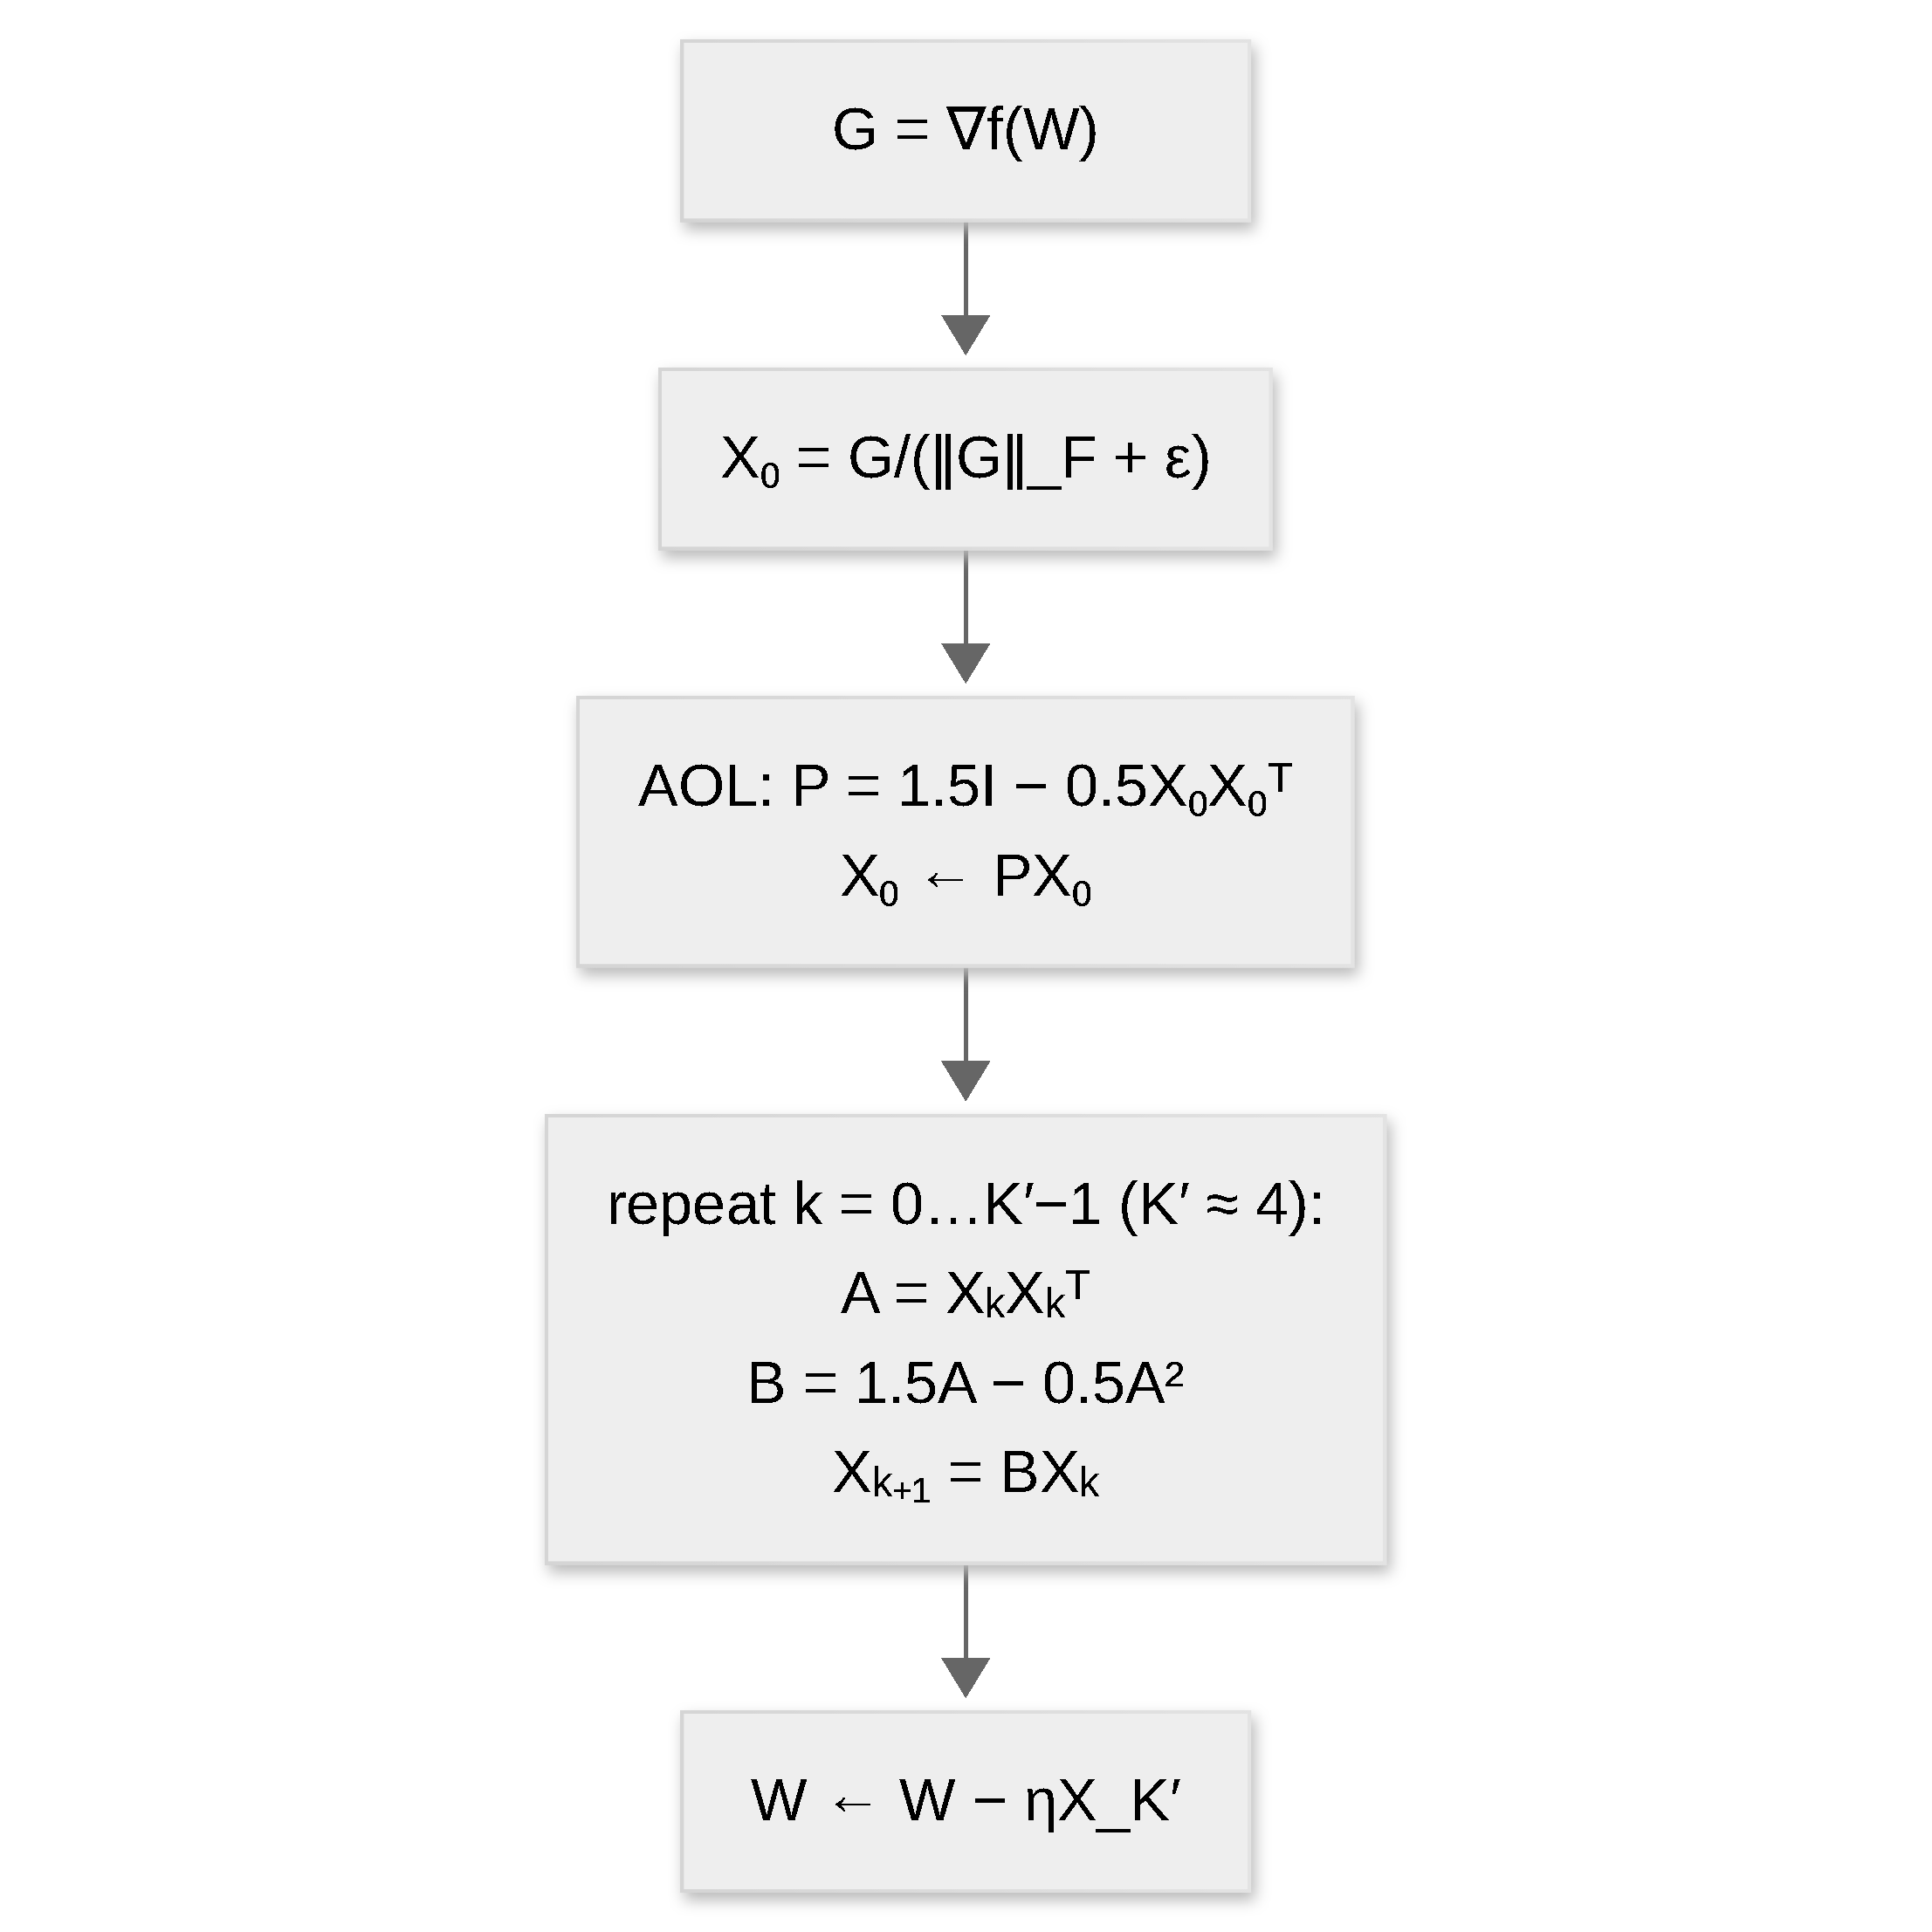
\includegraphics{figures/optimizers/turbo-muon.pdf}}
\caption{Step flow of Turbo-Muon: almost-orthogonal preconditioning (AOL) before the Newton-Schulz iterations, reducing their count.}
\label{fig:opt-turbo-muon}
\end{figure}
Turbo-Muon adds an \textbf{almost-orthogonal preconditioning} (AOL) step before the Newton-Schulz iterations. The preconditioner $P = 1.5I - 0.5X_0X_0^\top$ is applied to the normalized gradient, reducing the number of required orthogonalization steps to four while preserving the orthogonalized update geometry. It inherits Muon's hybrid routing: only hidden-layer 2D matrices are orthogonalized, while embedding tables, learned positional encodings, output heads and non-matrix parameters take decoupled AdamW updates.

\begin{algorithm}[H]
\caption{Turbo-Muon (AOL-Preconditioned Orthogonalization)}
\label{alg:turbo-muon}
\begin{algorithmic}[1]
\Require Initial parameters $\theta$, learning rate $\eta$, Newton-Schulz iters $K'$ (typically 4)
\Ensure Updated parameters $\theta_T$
\For{each parameter $P$}
    \If{$P$ is a hidden-layer 2D matrix $W$}
        \State $G \gets \nabla f(W)$ \Comment{Gradient}
        \State $X_0 \gets \frac{G}{\|G\|_F + \epsilon}$ \Comment{Normalize gradient}
        \State \textbf{AOL (Almost-Orthogonal preconditioner):} \Comment{Preconditioning step}
        \State $P \gets (1.5 I - 0.5 X_0 X_0^\top)$ \Comment{Preconditioning matrix}
        \State $X_0 \gets P X_0$ \Comment{Preconditioned start}
        \For{$k = 0, 1, \ldots, K'-1$}
            \State $A_k \gets X_k X_k^\top$
            \State $B_k \gets (3/2) A_k - (1/2) A_k^2$
            \State $X_{k+1} \gets B_k X_k$ \Comment{Reduced iterations due to AOL preconditioning}
        \EndFor
        \State $W \gets W - \eta X_{K'}$ \Comment{Update with preconditioned orthogonalized direction}
    \Else
        \State $P \gets \operatorname{AdamW}(P, \nabla f(P); \eta, \beta_1, \beta_2, \epsilon, \lambda)$ \Comment{Hybrid fallback: embeddings, pos, heads, non-matrices}
    \EndIf
\EndFor
\Return $\theta_T$
\end{algorithmic}
\end{algorithm}

\paragraph{Cons.}
\begin{itemize}[leftmargin=*]
\item Still compute-heavy; AOL adds a preconditioning matrix multiplication.
\item Requires the same custom-kernel support as Muon, and shares its dependence on the AdamW fallback for non-hidden parameter classes.
\end{itemize}

\paragraph{Pros.}
\begin{itemize}[leftmargin=*]
\item AOL reduces the Newton-Schulz iteration count (typically five to four).
\item Retains orthogonalized update geometry at lower iteration cost.
\end{itemize}

\paragraph{AF-Muon (AdamW-Free Tied-Embedding Muon).}
\begin{figure}[H]
\centering
\fitfigure{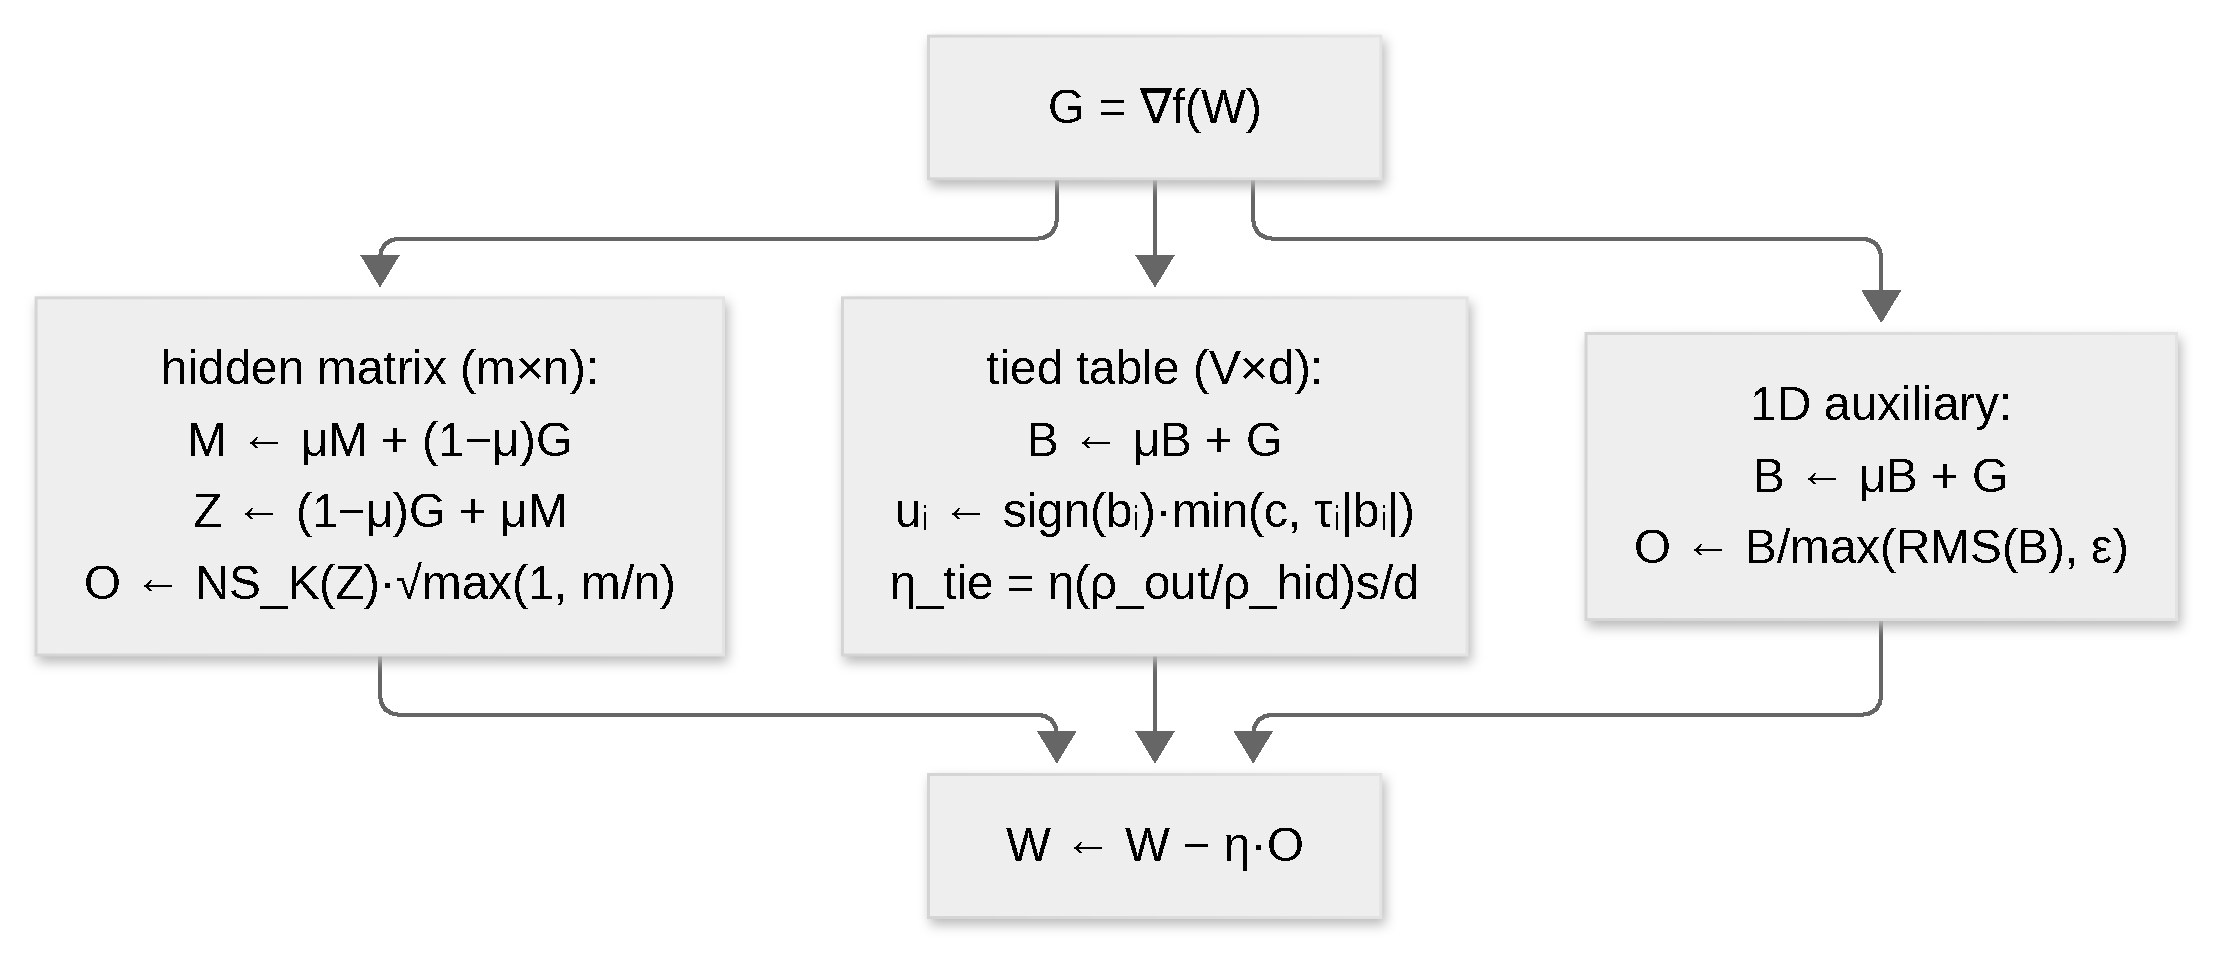
\includegraphics{figures/optimizers/af-muon.pdf}}
\caption{Step flow of AF-Muon: Muon's spectral update for hidden matrices, a support-aware finite-cap clipped-row LMO for the tied vocabulary table, and RMS-normalized updates for one-dimensional auxiliary parameters, all with a single first-moment buffer.}
\label{fig:opt-af-muon}
\end{figure}
AF-Muon is an \textbf{AdamW-free extension of Muon} that removes the auxiliary AdamW fallback of the Hybrid Muon recipe by giving every parameter class its own norm-constrained geometry. Hidden matrices keep the spectral update with a Nesterov signal; the vocabulary table, which simultaneously receives sparse input-lookup and dense output-softmax gradients, is updated row by row with a \emph{support-aware finite-cap linear minimization oracle}; one-dimensional auxiliary tensors receive an RMS-normalized update. No parameter class carries second-moment state, so a single first-moment buffer per parameter replaces the AdamW state of the hybrid recipe, which the authors report as roughly 20\% less optimizer-state memory at matched training.

For the tied table $W \in \mathbb{R}^{V \times d}$ with momentum row $b_i$, the oracle solves the row problem
\begin{align}
u_i &= \operatorname{sign}(b_i) \odot \min\left(c\,\mathbf{1},\ \tau_i\,|b_i|\right), \\
\|u_i\|_2^2 &= \min\left(d,\ c^2\,\bigl|\operatorname{supp}(b_i)\bigr|\right),
\end{align}
where the per-row scale $\tau_i$ is obtained by bisection in FP32 over complete-row chunks. Rows whose support cannot fill the row-$\ell_2$ radius saturate every useful coordinate at the cap $c$, so sparse lookup rows are handled without inflating absent coordinates. The cap interpolates between two known endpoints: $c = 1$ recovers the SCION-style Sign update and $c \geq \sqrt{d}$ reduces to a row-RMS update. The tied step size is $\eta_{tie} = \eta_M (\rho_{out}/\rho_{hid})\, s / d$; the paper's main setting is $c = 3$ and $s = 0.5$ with $\rho_{out}/\rho_{hid} = 60$, and its diagnostics report the finite cap active on under 0.3\% of coordinates while affecting most rows.

\begin{algorithm}[H]
\caption{AF-Muon (AdamW-Free Tied-Embedding Muon)}
\label{alg:af-muon}
\begin{algorithmic}[1]
\Require Initial parameters $\theta$, matrix LR $\eta_M$, vector LR $\eta_{vec}$, momentum $\mu$, matrix weight decay $\lambda_M$, tied scale $s$, cap $c$, radii $\rho_{out}, \rho_{hid}$, Newton-Schulz iters $K$
\Ensure Updated parameters $\theta_T$
\For{each parameter tensor $W$ with gradient $G_t$}
    \If{$W$ is a hidden matrix in $\mathbb{R}^{m \times n}$}
        \State $M_t \gets \mu M_{t-1} + (1-\mu) G_t$ \Comment{First moment}
        \State $Z_t \gets (1-\mu) G_t + \mu M_t$ \Comment{Nesterov signal}
        \State $O_t \gets \mathrm{NS}_K(Z_t)\sqrt{\max(1, m/n)}$ \Comment{Spectral update}
        \State $W_t \gets (1 - \eta_M \lambda_M) W_{t-1} - \eta_M O_t$
    \ElsIf{$W \in \mathbb{R}^{V \times d}$ is the tied vocabulary table}
        \State $B_t \gets \mu B_{t-1} + G_t$ \Comment{Unnormalized first moment}
        \State $\eta_{tie,t} \gets \eta_M (\rho_{out}/\rho_{hid}) s / d$
        \For{each row $i = 1, \ldots, V$}
            \State $u_i \gets L_c\bigl(\mathrm{row}_i(B_t)\bigr)$ \Comment{Capped-row LMO}
        \EndFor
        \State $W_t \gets W_{t-1} - \eta_{tie,t} U$
    \Else
        \State $B_t \gets \mu B_{t-1} + G_t$ \Comment{$1$D auxiliary tensor}
        \State $O_t \gets B_t / \max(\mathrm{RMS}(B_t), \epsilon)$
        \State $W_t \gets W_{t-1} - \eta_{vec} O_t$
    \EndIf
\EndFor
\Return $\theta_T$
\end{algorithmic}
\end{algorithm}

\paragraph{Cons.}
\begin{itemize}[leftmargin=*]
\item Every parameter must be assigned an explicit role (matrix, tied table, or vector); an untied output head or an extra embedding table is not a tied-table block.
\item The tied-table oracle requires a per-row bisection with complete-row chunking; the paper reports roughly 1\% median step-time overhead at matched training.
\item The tied-table claim is established for tied-vocabulary models; frontier-scale pretraining and universal endpoint superiority are not claimed.
\end{itemize}

\paragraph{Pros.}
\begin{itemize}[leftmargin=*]
\item AdamW-free: one first-moment buffer per parameter and no second-moment state, reported as roughly 20\% less optimizer-state memory than Hybrid Muon.
\item The finite cap preserves within-row magnitudes while bounding coordinate concentration, and recovers Sign ($c=1$) and row-RMS ($c \geq \sqrt{d}$) as limit cases.
\item Improves mean validation loss and perplexity over both Hybrid Muon and a SCION-style Sign endpoint across nine tied-token settings spanning text, image-token, protein, MoE, and encoder-decoder models.
\end{itemize}

\paragraph{AdaMuon (Adaptive Muon).}
AdaMuon is an \textbf{adaptive extension of Muon} that keeps the spectral (polar) update while adding coordinate-wise variance normalization. Muon orthogonalizes the momentum matrix into a direction-only update, which removes anisotropic scaling but assigns the same magnitude to every coordinate; AdaMuon addresses the resulting mismatch between noisy and informative coordinates by tracking the element-wise variance of the \emph{orthogonalized} direction rather than of the raw gradient or of the momentum. Because the polar factor is globally scale-invariant, the sign transform applied before orthogonalization preserves the update direction while stabilizing its element-wise magnitudes; the paper proves that $\operatorname{sign}$ is the unique element-wise map that is scale-free, sign-consistent, odd and bounded (Theorem~1). The second-moment estimate therefore sees a stable signal, and its variance-normalized version is rescaled to an RMS of $0.2$, matching Adam's empirical update scale so that existing learning-rate schedules are reused without tuning.

For a weight $W_t \in \mathbb{R}^{n \times m}$, momentum buffer $M_t$, momentum $\beta$, Newton--Schulz steps $T$ and small constant $\varepsilon$:
\begin{align}
M_t &= \beta M_{t-1} + G_t, \\
O_t &= \operatorname{NewtonSchulz}\bigl(\operatorname{sign}(M_t), T\bigr), \\
V_t &= \beta V_{t-1} + (1-\beta)\, O_t \odot O_t, \\
\widehat{O}_t &= O_t \oslash \bigl(\sqrt{V_t} + \varepsilon \mathbf{1}\bigr), \\
\gamma_t &= \frac{0.2\sqrt{mn}}{\|\widehat{O}_t\|_F}, \\
W_{t+1} &= W_t - \eta\bigl(\gamma_t \widehat{O}_t + \lambda W_t\bigr).
\end{align}
The Newton--Schulz map uses $X_0 = \operatorname{sign}(M_t)/\|\operatorname{sign}(M_t)\|_F$ and the cubic iteration $X_k = aX_{k-1} + b(X_{k-1}X_{k-1}^{\mathsf T})X_{k-1} + c(X_{k-1}X_{k-1}^{\mathsf T})^2X_{k-1}$ with $(a,b,c) = (3.4445, -4.7750, 2.0315)$ and $T = 5$. No bias correction is applied to either moment: a constant factor in $V_t$ is cancelled exactly by $\gamma_t \propto \sqrt{c}$, and a constant factor in $M_t$ is removed by the polar map, $\operatorname{polar}(cM) = \operatorname{polar}(M)$.

\begin{algorithm}[H]
\caption{AdaMuon (Adaptive Muon)}
\label{alg:ada-muon}
\begin{algorithmic}[1]
\Require Initial weights $W_0 \in \mathbb{R}^{n \times m}$, learning rate $\eta$, weight decay $\lambda$, momentum $\beta$, Newton--Schulz steps $T$, small constant $\varepsilon$
\Ensure Updated weights $W_T$
\State $M_0 \gets \mathbf{0}$, $V_0 \gets \mathbf{0}$
\For{each iteration $t = 1, 2, \ldots$}
    \State $G_t \gets \nabla_{W_t}\mathcal{L}(W_t)$
    \State $M_t \gets \beta M_{t-1} + G_t$
    \State $O_t \gets \operatorname{NewtonSchulz}(\operatorname{sign}(M_t), T)$
    \State $V_t \gets \beta V_{t-1} + (1-\beta)\, O_t \odot O_t$
    \State $\widehat{O}_t \gets O_t \oslash (\sqrt{V_t} + \varepsilon\mathbf{1})$
    \State $\gamma_t \gets 0.2\sqrt{mn}/\|\widehat{O}_t\|_F$
    \State $W_{t+1} \gets W_t - \eta(\gamma_t \widehat{O}_t + \lambda W_t)$
\EndFor
\Return $W_T$
\end{algorithmic}
\end{algorithm}

\paragraph{Cons.}
\begin{itemize}[leftmargin=*]
\item One additional second-moment buffer per matrix parameter (two buffers versus Muon's single first-moment buffer), plus per-step element-wise EMA, square-root and normalization work on the update.
\item The update is defined for two-dimensional parameters; one-dimensional parameters (biases, norm scales) require an auxiliary optimizer in the paper's recipe.
\item The RMS target ($0.2$) is a fixed constant rather than a learned quantity, so the method assumes Adam-like update scales when reusing existing schedules.
\end{itemize}

\paragraph{Pros.}
\begin{itemize}[leftmargin=*]
\item No new hyperparameters: the second-moment EMA reuses Muon's momentum coefficient $\beta$, and the paper reports low sensitivity across $\beta \in [0.8, 0.99]$.
\item The sign transform makes the variance estimate stable enough to normalize, and the RMS alignment cancels any constant bias in $V_t$, so no bias correction is needed for either moment.
\item RMS alignment matches Adam's update scale, allowing direct reuse of learning-rate schedules; the authors report up to roughly 40\% training-efficiency gains over AdamW and consistent wins over Muon on GPT-2 (125M--1.5B) and Qwen2.5 (1.5B, 7B).
\end{itemize}

\paragraph{Dion3 (Fractional Gram-Newton-Schulz Orthogonalization).}
Dion3~\citep{amsel_dion3_2026} is a \textbf{revision of Muon} that reduces the cost of the orthogonalization step at the algorithmic level. It replaces standard Newton--Schulz with \emph{Gram Newton--Schulz}, a mathematically equivalent iteration that runs on the small symmetric Gram matrix $XX^{\mathsf T}$, and it orthogonalizes only a fraction $f \in (0,1]$ of the momentum rows at each step, updating only those rows of the weight matrix. \emph{Error feedback} decays only the selected rows of the momentum buffer, so rows that were not selected keep accumulating and are eventually chosen. At $f = 1$ the update reduces to Muon in exact arithmetic (or to NorMuon with the optional row-wise normalization). For a weight $W \in \mathbb{R}^{n \times m}$ (operating on the smaller dimension, $n \le m$), fraction $f$, $k = \lceil f n \rceil$, momentum $\mu$, learning rate $\eta$ and weight decay $\lambda$:
\begin{align}
M_t &= M_{t-1} + G_t \quad\text{(momentum accumulation; damping deferred)} \\
S_t &= \operatorname{topk}_{i}\bigl(\lVert M_{t,i,:}\rVert_1,\ k\bigr) \quad\text{(select the } k \text{ largest rows)} \\
O_t &= \operatorname{GramNS}\bigl(M_t[S_t,:]\bigr) \quad\text{(orthogonalize the } k \times m \text{ submatrix)} \\
W_t &= (1 - \eta\lambda)\, W_{t-1}, \qquad W_t[S_t,:] \gets W_t[S_t,:] - \eta\, O_t \\
M_t[S_t,:] &\gets \mu\, M_t[S_t,:] \quad\text{(error feedback: decay only selected rows)}
\end{align}
Gram Newton--Schulz normalizes $X \gets M_t[S_t,:]/(\lVert M_t[S_t,:]\rVert_F + \epsilon)$ with $\epsilon = 10^{-7}$, casts to \texttt{float16}, forms $R_0 = X X^{\mathsf T}$ and $Q_0 = I$, and runs $T$ iterations
\begin{align}
Z_t &= b_t R_{t-1} + c_t R_{t-1}^2, &
Q_t &= Q_{t-1} Z_t + a_t Q_{t-1}, \\
(RZ)_t &= R_{t-1} Z_t + a_t R_{t-1}, &
R_t &= Z_t (RZ)_t + a_t (RZ)_t,
\end{align}
returning $Q_T X$. A \emph{restart} after iteration~2 ($X \gets Q_2 X$, $R_2 \gets X X^{\mathsf T}$, $Q_2 \gets I$) removes the spurious negative eigenvalues that half precision introduces in the Gram matrix; the coefficients $(a_t,b_t,c_t)$ are the Polar Express five-step triples~\citep{amsel_polar_express_2026}. The cost falls from $T(3\alpha+1)n^3$ FLOPs for standard Newton--Schulz to $(4T+3\alpha-3)n^3$ for Gram Newton--Schulz ($\alpha = m/n$), and selecting $k = \lceil f n \rceil$ rows both shrinks the iteration and raises the aspect ratio by $1/f$. The optional NorMuon flavor adds a row-wise second moment $v_i \gets \beta_2 v_i + (1-\beta_2)\,\operatorname{mean}_j(O_{ij}^2)$ for $i \in S$, rescales $\tilde O_{ij} = O_{ij}/(\sqrt{v_i}+\epsilon)$, and renormalizes $\tilde O \gets \tilde O\,\lVert O\rVert_F/\lVert\tilde O\rVert_F$ in \texttt{float32} before the update.

\begin{algorithm}[H]
\caption{Dion3 (Fractional Orthogonalization with Error Feedback)}
\label{alg:dion3}
\begin{algorithmic}[1]
\Require Matrices $W$, learning rate $\eta$, momentum $\mu$, fraction $f$, Gram Newton--Schulz steps $T$, $\epsilon$, weight decay $\lambda$
\Ensure Updated matrices $W_T$
\For{each 2D parameter matrix $W$ with gradient $G$}
    \State $M \gets M + G$ \Comment{Momentum accumulation}
    \State $S \gets$ indices of the $k = \lceil f n \rceil$ rows of $M$ with largest $\ell_1$ norm \Comment{Selection}
    \State $O \gets \operatorname{GramNS}_T(M[S,:])$ \Comment{Orthogonalize the selected submatrix}
    \If{NorMuon}
        \State $v_i \gets \beta_2 v_i + (1-\beta_2)\operatorname{mean}_j(O_{ij}^2)$ for $i \in S$
        \State $\tilde O_{ij} \gets O_{ij}/(\sqrt{v_i}+\epsilon)$; \quad $\tilde O \gets \tilde O\,\lVert O\rVert_F/\lVert\tilde O\rVert_F$
    \EndIf
    \State $W \gets (1 - \eta\lambda) W$ \Comment{Weight decay on all rows}
    \State $W[S,:] \gets W[S,:] - \eta\,\tilde O$ \Comment{Update selected rows only}
    \State $M[S,:] \gets \mu\, M[S,:]$ \Comment{Error feedback}
\EndFor
\Return $W_T$
\end{algorithmic}
\end{algorithm}

\paragraph{Cons.}
\begin{itemize}[leftmargin=*]
\item Each step updates only a fraction of the rows, so the optimization trajectory differs from Muon; the paper reports the change is benign (Section~8.1 of the Dion3 report).
\item Row selection and error feedback add top-$k$ bookkeeping and a row-wise momentum decay per step.
\item The largest wall-clock gains in the paper come from symmetric GEMM kernels and megabatched communication, which are hardware- and cluster-specific; only the algorithmic reduction and the single first-moment buffer apply here.
\end{itemize}

\paragraph{Pros.}
\begin{itemize}[leftmargin=*]
\item Gram Newton--Schulz is mathematically equivalent to Newton--Schulz and cuts orthogonalization FLOPs by about 55\% at typical transformer aspect ratios with five iterations.
\item Fractional row selection reduces the orthogonalized submatrix to $k \times m$ and raises its aspect ratio by $1/f$, compounding the Gram savings; the paper reports up to $6\times$ faster optimizer steps at matched loss.
\item At $f = 1$ the update reduces to Muon (or NorMuon), and a single momentum buffer per matrix parameter suffices; error feedback lets ignored rows participate eventually.
\end{itemize}

\paragraph{ROOT (Robust Orthogonalized Optimizer).}
\begin{figure}[H]
\centering
\fitfigure{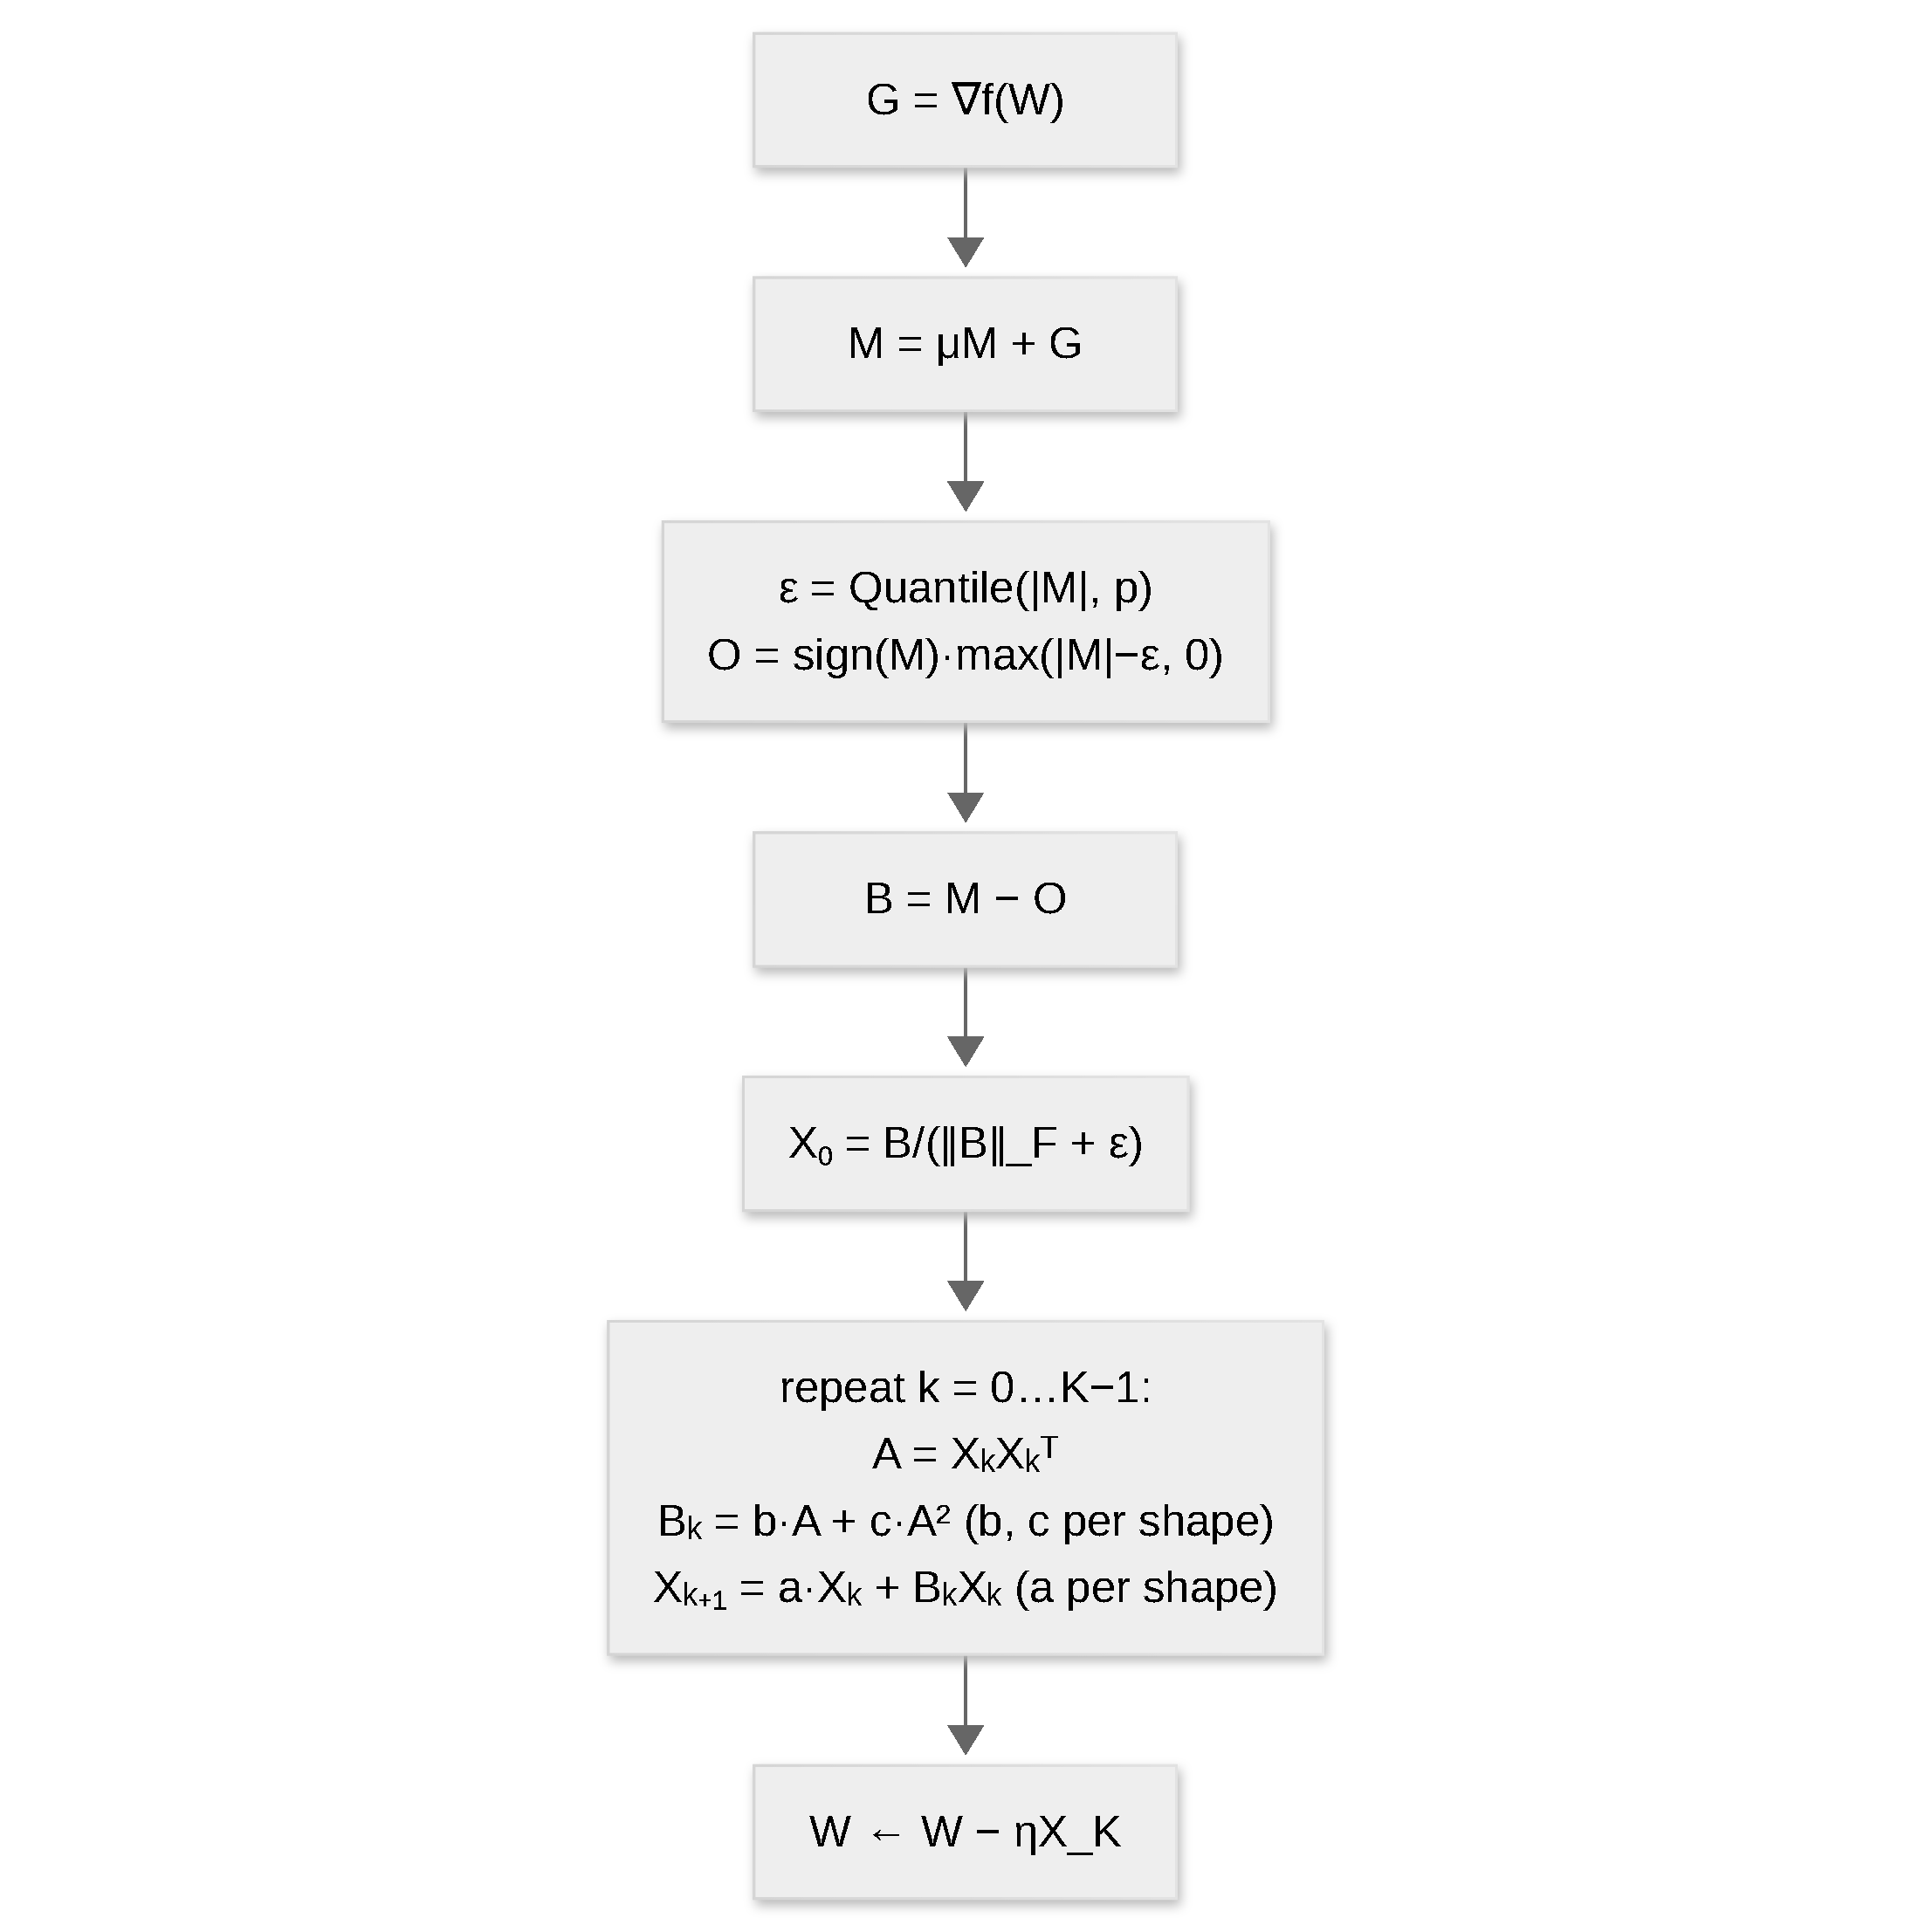
\includegraphics{figures/optimizers/root.pdf}}
\caption{Step flow of ROOT: momentum accumulation, soft-threshold outlier separation, and shape-calibrated Newton--Schulz orthogonalization.}
\label{fig:opt-root}
\end{figure}
ROOT~\citep{he_root_2025} is a \textbf{robustness-oriented revision of Muon} that attacks two fragilities of the fixed-coefficient Newton--Schulz pipeline. First, the universal coefficients $(a,b,c)=(3.4445,-4.7750,2.0315)$ are calibrated for an ``average'' matrix shape and lose precision exactly on square and near-square layers: the orthogonalization MSE ranges from $0.0499$ at $2048\times2048$ to $0.0003$ at $2048\times16384$ in Table~1 of the paper. ROOT replaces them with per-shape coefficients $\{a^{(m,n)}, b^{(m,n)}, c^{(m,n)}\}$ calibrated offline over momentum singular-value distributions (Mixed 1:3 real-to-random calibration), a scheme the authors call \emph{AdaNewton}. Second, heavy-tailed gradient components distort the Frobenius normalization required by Newton--Schulz and are amplified by the polynomial iteration; ROOT models the momentum as $M_t = B_t + O_t$ and solves a proximal L1 problem whose closed-form solution is soft-thresholding. Only the robust base component $B_t$ is orthogonalized; the sparse outlier component $O_t$ is discarded. For a hidden-layer weight matrix $W \in \mathbb{R}^{m\times n}$, momentum $\mu$, learning rate $\eta$, percentile $p$ and iteration count $K$:
\begin{align}
M_t &= \mu M_{t-1} + \nabla \mathcal{L}(\theta_{t-1}) \quad\text{(momentum, Eq. 1)} \\
\varepsilon_t &= \operatorname{Quantile}(|M_t|, p) \quad\text{(dynamic threshold, } p=0.90 \text{ default)} \\
O_t &= \mathcal{T}_{\varepsilon_t}[M_t], \quad \mathcal{T}_\varepsilon[x]_i = \operatorname{sign}(x_i)\max(|x_i|-\varepsilon, 0) \quad\text{(soft-threshold, Eqs. 7--10)} \\
B_t &= M_t - O_t \quad\text{(clipped robust component, Eq. 9)} \\
X_0 &= \frac{B_t}{\lVert B_t\rVert_F}, \qquad X_k = a^{(m,n)}X_{k-1} + b^{(m,n)}X_{k-1}(X_{k-1}^\top X_{k-1}) + c^{(m,n)}X_{k-1}(X_{k-1}^\top X_{k-1})^2 \\
\theta_t &= \theta_{t-1} - \eta X_K \quad\text{(update, } K=5\text{)}
\end{align}

\begin{table}[H]
\centering
\caption{AdaNewton coefficients from Table~1 of \citet{he_root_2025} (Mixed 1:3 calibration). Shapes outside the table fall back to Muon's fixed $(3.4445,-4.7750,2.0315)$.}
\label{tab:root-coefficients}
\small
\begin{tabular}{rrrrrr}
\toprule
$m$ & $n$ & $a^{(m,n)}$ & $b^{(m,n)}$ & $c^{(m,n)}$ & MSE \\
\midrule
2048 & 2048 & 3.3334 & $-4.2591$ & 1.7791 & 0.0352 \\
4096 & 4096 & 3.3732 & $-4.6134$ & 2.0576 & 0.0470 \\
8192 & 8192 & 3.3886 & $-4.9026$ & 2.3105 & 0.0587 \\
3072 & 2048 & 2.9091 & $-3.8108$ & 1.8600 & 0.0024 \\
4096 & 2048 & 2.7739 & $-3.4911$ & 1.6992 & 0.0010 \\
8192 & 2048 & 2.5925 & $-3.0010$ & 1.4138 & 0.0003 \\
16384 & 2048 & 2.7045 & $-3.2335$ & 1.5336 & 0.0003 \\
\bottomrule
\end{tabular}
\end{table}

\begin{algorithm}[H]
\caption{ROOT (Robust Orthogonalized Optimizer)}
\label{alg:root}
\begin{algorithmic}[1]
\Require Initial parameters $\theta$, learning rate $\eta$, momentum $\mu$, percentile $p$, Newton--Schulz iters $K$
\Ensure Updated parameters $\theta_T$
\For{each parameter $P$}
    \If{$P$ is a hidden-layer 2D matrix $W$}
        \State $G \gets \nabla f(W)$ \Comment{Gradient}
        \State $M \gets \mu M + G$ \Comment{Momentum accumulation}
        \State $\varepsilon \gets \operatorname{Quantile}(|M|, p)$ \Comment{Dynamic threshold}
        \State $O \gets \operatorname{sign}(M)\max(|M|-\varepsilon, 0)$ \Comment{Outlier separation (soft-threshold)}
        \State $B \gets M - O$ \Comment{Clipped robust component}
        \State $X_0 \gets \frac{B}{\|B\|_F + \epsilon}$ \Comment{Normalize by Frobenius norm}
        \For{$k = 0, 1, \ldots, K-1$}
            \State $A_k \gets X_k X_k^\top$ \Comment{Gramian}
            \State $B_k \gets b^{(m,n)} A_k + c^{(m,n)} A_k^2$ \Comment{Shape-calibrated coefficients}
            \State $X_{k+1} \gets a^{(m,n)} X_k + B_k X_k$ \Comment{Polynomial step}
        \EndFor
        \State $W \gets W - \eta X_K$ \Comment{Update with orthogonalized direction}
    \Else
        \State $P \gets \operatorname{AdamW}(P, \nabla f(P); \eta, \beta_1, \beta_2, \epsilon, \lambda)$ \Comment{Hybrid fallback: embeddings, pos, heads, non-matrices}
    \EndIf
\EndFor
\Return $\theta_T$
\end{algorithmic}
\end{algorithm}

Following the hybrid recipe of Muon, only hidden-layer 2-D matrices take the ROOT path; embedding tables, learned positional encodings, output heads and every non-matrix parameter are trained with decoupled AdamW using the group-level learning rate, weight decay, $\beta_1, \beta_2$ and $\epsilon$ settings. The paper's LLM runs apply a $0.2$ update-RMS scaling factor following Moonlight; this implementation lets the per-group learning rates absorb that calibration, so no scale constant is applied. Shapes absent from Table~\ref{tab:root-coefficients} fall back to Muon's fixed coefficients, and the dynamic quantile costs an additional sort of $|M_t|$ per matrix per step.

\paragraph{Cons.}
\begin{itemize}[leftmargin=*]
\item The percentile threshold requires an $O(N\log N)$ sort of the momentum matrix at every step, on top of the Newton--Schulz matmuls.
\item The calibrated coefficient table covers seven shapes only; every other shape falls back to Muon's fixed coefficients.
\item Outliers are discarded rather than shrunk, so an extremely noisy gradient can also lose informative signal; the paper's ablation shows the trade-off is governed by the percentile (0.85 truncates too much, 0.99 too little).
\end{itemize}

\paragraph{Pros.}
\begin{itemize}[leftmargin=*]
\item Dimension-invariant orthogonalization precision: shape-calibrated coefficients remove the precision cliff that fixed coefficients show on square and near-square layers.
\item Outlier-robust without retuning the Muon recipe; the paper reports lower loss and a better zero-shot average than Muon and AdamW at 1B scale (60.12 vs 59.59 vs 59.05) and gains on ViT/CIFAR-10.
\item Same single momentum buffer per matrix parameter as Muon, and the \texttt{softthresh}/\texttt{ada\_newton} toggles expose the paper's ablations directly.
\end{itemize}

\paragraph{Muon² (Second-Moment Preconditioned Orthogonalization).}
Muon$^2$~\citep{liu_muon2_2026} generalizes Muon by preconditioning the momentum with an
\textbf{Adam-style second-moment EMA before the Newton--Schulz orthogonalization}. The
paper shows that the practical bottleneck of Muon's polar approximation is the
ill-conditioned momentum matrix (early-training spectra span $10^{-4}$--$1$ with roughly
half the singular values in the NS ``dead zone''); dividing by $\sqrt{V_t}$ tightens the
spectrum, so every NS step aligns better with the true orthogonalized update (cosine
similarity $0.916$ at $K{=}3$ vs Muon's $0.931$ at $K{=}5$, rising to $0.975$ at
$K{=}5$). For a hidden-layer weight matrix $W \in \mathbb{R}^{n \times m}$ with learning
rate $\eta$:
\begin{align}
M_t &= \beta_1 M_{t-1} + (1-\beta_1) G_t && \text{(momentum EMA, Eq.~2)} \\
V_t &= \beta_2 V_{t-1} + (1-\beta_2)\, (G_t \odot G_t) && \text{(second-moment EMA, Eq.~3)} \\
\widetilde{M}_t &= M_t \oslash \big(\sqrt{V_t} + \epsilon \mathbf{1}\big) && \text{(preconditioning, Eq.~4)} \\
X_0 &= \frac{\widetilde{M}_t}{\|\widetilde{M}_t\|_F + \epsilon}, \qquad
X_{k+1} = aX_k + b\, X_k X_k^\top X_k + c\, X_k (X_k X_k^\top)^2 X_k && \text{(NS, Eq.~5)} \\
W_{t+1} &= W_t - \eta \sqrt{m/n}\, X_K && \text{(update, Eq.~6)}
\end{align}
with the same quintic coefficients $(a,b,c)=(3.4445,-4.7750,2.0315)$ as Muon and the
$\sqrt{m/n}$ learning-rate factor proposed by Bernstein (2025). The memory-efficient
variant \textbf{Muon$^2$-F} replaces $V_t$ with Adafactor-style row/column statistics:
\begin{align}
r_t &= \beta_2 r_{t-1} + (1-\beta_2)\,\mathrm{sum}_{\mathrm{col}}(G_t \odot G_t), \qquad
c_t = \beta_2 c_{t-1} + (1-\beta_2)\,\mathrm{sum}_{\mathrm{row}}(G_t \odot G_t), \\
\widehat{V}_t &= \frac{r_t\, c_t^\top}{\mathrm{sum}(r_t)},
\end{align}
keeping memory within $\sim$0.3\% of Muon at 7B scale (47.53 vs 47.29 GB) while retaining
most of Muon$^2$'s benefit. Across GPT, LLaMA and Mixture-of-Experts pre-training up to
13B parameters, Muon$^2$ outperforms Muon at equal NS iterations and matches it with
$K{=}3$ instead of $5$ (a 40\% reduction), saving up to a quarter of training time at
equal loss.

\begin{algorithm}[H]
\caption{Muon² (Second-Moment Preconditioned Orthogonalization)}
\label{alg:muon2}
\begin{algorithmic}[1]
\Require Initial parameters $\theta$, learning rate $\eta$, $\beta_1, \beta_2$, NS iters $K$, preconditioner $\epsilon$
\Ensure Updated parameters $\theta_T$
\For{each parameter $P$}
    \If{$P$ is a hidden-layer 2D matrix $W \in \mathbb{R}^{n\times m}$}
        \State $G \gets \nabla f(W)$ \Comment{Gradient}
        \State $M \gets \beta_1 M + (1-\beta_1) G$ \Comment{Momentum EMA (Eq.~2)}
        \State $V \gets \beta_2 V + (1-\beta_2) (G \odot G)$ \Comment{Second-moment EMA (Eq.~3); factored variant keeps row/col sums only}
        \State $\widetilde{M} \gets M \oslash (\sqrt{V} + \epsilon\mathbf{1})$ \Comment{Precondition (Eq.~4)}
        \State $X_0 \gets \widetilde{M} / (\|\widetilde{M}\|_F + \epsilon)$ \Comment{Frobenius normalization}
        \For{$k = 0, 1, \ldots, K-1$}
            \State $A_k \gets X_k X_k^\top$ \Comment{Gramian}
            \State $X_{k+1} \gets 3.4445\,X_k - 4.7750\,A_k X_k + 2.0315\,A_k^2 X_k$ \Comment{Quintic NS step}
        \EndFor
        \State $W \gets W - \eta \sqrt{m/n}\, X_K$ \Comment{Scaled update (Eq.~6)}
    \Else
        \State $P \gets \operatorname{AdamW}(P, \nabla f(P); \eta, \beta_1, \beta_2, \epsilon, \lambda)$ \Comment{Hybrid fallback: embeddings, pos, heads, non-matrices}
    \EndIf
\EndFor
\Return $\theta_T$
\end{algorithmic}
\end{algorithm}

Following the hybrid recipe of Muon, only hidden-layer 2-D matrices take the Muon$^2$
path; embedding tables, learned positional encodings, output heads and every non-matrix
parameter are trained with decoupled AdamW using the group-level learning rate, weight
decay, $\beta_1, \beta_2$ and $\epsilon$ settings --- the same $\beta_1, \beta_2, \epsilon$
also parameterize Eqs.~2--4, so one per-group knob set configures both paths.

\paragraph{Cons.}
\begin{itemize}[leftmargin=*]
\item One extra full-size state buffer over Muon (two moment EMAs per matrix), doubling
optimizer memory on the orthogonalized path unless the factored variant is enabled.
\item The $\sqrt{m/n}$ update scale differs from this repository's plain \texttt{muon}
path, so learning rates do not transfer one-to-one between the two registry entries.
\item $\beta_1, \beta_2$ defaults are not fixed by the paper; this implementation inherits
the shared per-group defaults $(0.9, 0.95)$.
\end{itemize}

\paragraph{Pros.}
\begin{itemize}[leftmargin=*]
\item Better orthogonalization at equal NS iterations and equal quality with 40\% fewer
iterations (3 instead of 5), cutting NS compute and communication.
\item Consistent gains over Muon across GPT, LLaMA and Mixture-of-Experts pre-training up
to 13B parameters, with up to a quarter of training time saved at matched loss.
\item The \texttt{factored} toggle exposes Muon$^2$-F, which keeps memory within
$\sim$0.3\% of Muon while preserving most of the benefit.
\end{itemize}

\paragraph{NorMuon (Neuron-wise Normalized Muon).}
NorMuon~\citep{li_normuon_2025} keeps Muon's orthogonalized update and adds a
\textbf{neuron-wise (row-wise) adaptive learning rate} on top of it. Muon's
Newton--Schulz iteration equalizes the singular values of the update, but the $L_2$ norm
of the individual neuron rows remains highly non-uniform: some neurons receive
disproportionately large updates while others are barely trained. NorMuon tracks the
mean squared magnitude of each row of the \emph{orthogonalized} direction in a
second-moment EMA, divides every neuron row by its RMS, and rescales the whole update to
Adam's empirical update scale so existing learning-rate schedules transfer unchanged.
For a hidden-layer weight matrix $W \in \mathbb{R}^{m \times n}$ with learning rate
$\eta$:
\begin{align}
M_t &= \beta_1 M_{t-1} + (1-\beta_1) G_t && \text{(momentum, line 5)} \\
O_t &= \mathrm{NS}_5(M_t) && \text{(orthogonalization, line 6)} \\
v_t &= \beta_2 v_{t-1} + (1-\beta_2)\,\mathrm{mean}_{\mathrm{cols}}(O_t \odot O_t) && \text{(neuron EMA, line 7)} \\
V_t &= \mathrm{ExpandRows}(v_t), \qquad \widehat{O}_t = O_t \oslash \big(\sqrt{V_t} + \epsilon\big) && \text{(row normalization, lines 8--9)} \\
\hat\eta &= \frac{0.2\,\eta\,\sqrt{mn}}{\lVert \widehat{O}_t \rVert_F}, \qquad
W_{t+1} = W_t - \eta\lambda W_t - \hat\eta\,\widehat{O}_t && \text{(update, lines 10--11)}
\end{align}
with $v_t \in \mathbb{R}^m$ (one scalar per neuron) and the same quintic Newton--Schulz
coefficients $(a,b,c)=(3.4445,-4.7750,2.0315)$ as Muon. The per-neuron statistic costs
$m$ scalars against the $m \times n$ first moment, so optimizer state is $m(n+1)$ ---
within a $1/n$ factor of Muon and roughly half of Adam's $2mn$. On 1.1B and 5.4B
pretraining NorMuon needs 21.74\% and 13.91\% fewer steps than AdamW to reach the same
validation loss; on Modded-NanoGPT (124M/350M) it reaches Muon's loss with 6\% and 15\%
fewer iterations, at a 2.9\% training-step-time overhead over AdamW and 21.19 GB of
optimizer state versus 40.56 GB for AdamW at 5.4B.

\begin{algorithm}[H]
\caption{NorMuon (Neuron-wise Normalized Muon)}
\label{alg:normuon}
\begin{algorithmic}[1]
\Require Initial parameters $\theta$, learning rate $\eta$, $\beta_1, \beta_2$, NS iters $K$, row-normalization $\epsilon$, weight decay $\lambda$
\Ensure Updated parameters $\theta_T$
\For{each parameter $P$}
    \If{$P$ is a hidden-layer 2D matrix $W \in \mathbb{R}^{m\times n}$}
        \State $G \gets \nabla f(W)$ \Comment{Gradient}
        \State $M \gets \beta_1 M + (1-\beta_1) G$ \Comment{Momentum (line 5)}
        \State $O \gets \mathrm{NS}_K(M)$ \Comment{Newton--Schulz (line 6)}
        \State $v \gets \beta_2 v + (1-\beta_2)\,\mathrm{mean}_{\mathrm{cols}}(O \odot O)$ \Comment{Per-neuron second moment (line 7)}
        \State $\widehat{O} \gets O \oslash (\sqrt{\mathrm{ExpandRows}(v)} + \epsilon\mathbf{1})$ \Comment{Row normalization (lines 8--9)}
        \State $\hat\eta \gets 0.2\,\eta\,\sqrt{mn} / (\|\widehat{O}\|_F + \epsilon)$ \Comment{RMS alignment (line 10)}
        \State $W \gets (1-\eta\lambda)\,W - \hat\eta\,\widehat{O}$ \Comment{Update (line 11)}
    \Else
        \State $P \gets \operatorname{AdamW}(P, \nabla f(P); \eta, \beta_1, \beta_2, \epsilon, \lambda)$ \Comment{Hybrid fallback: embeddings, pos, heads, non-matrices}
    \EndIf
\EndFor
\Return $\theta_T$
\end{algorithmic}
\end{algorithm}

Following the hybrid recipe of Muon, only hidden-layer 2-D matrices take the NorMuon
path; embedding tables, learned positional encodings, output heads and every non-matrix
parameter are trained with decoupled AdamW using the group-level learning rate, weight
decay, $\beta_1, \beta_2$ and $\epsilon$ settings. This implementation maps the paper's
parameters to the registry as follows: the \texttt{momentum} suffix is $\beta_1$, the
shared per-group \texttt{betas[1]} is $\beta_2$, the shared per-group \texttt{eps} is
$\epsilon$, and \texttt{ns\_steps}/\texttt{ns\_eps} drive the Newton--Schulz iteration.
Because NS5 starts with a Frobenius normalization, the paper's $(1-\beta_1)$ momentum
scaling and this repository's standard momentum accumulation produce identical updates.
The paper's second contribution, Algorithm~2, distributes the orthogonalization across
FSDP2 ranks (round-robin parameter assignment, gather/NS5/scatter, shard-local row
normalization) to avoid replicated work; that deployment strategy is orthogonal to the
update rule and is not implemented here.

\paragraph{Cons.}
\begin{itemize}[leftmargin=*]
\item One extra per-row state vector per matrix parameter (stored in float32); small
next to the $m \times n$ momentum, but non-zero.
\item The normalization must follow orthogonalization: the paper's ``NorMuon (Front)''
ablation, which applies it before NS5, is slightly worse.
\item $\epsilon$ is placed outside the root ($\sqrt{V_t}+\epsilon$), following
Algorithm~2; Algorithm~1's rendering of line 9 is typographically ambiguous.
\item The neuron-wise statistics do not replace the AdamW fallback: embeddings, pos,
heads and non-2-D tensors still carry full first/second moments.
\end{itemize}

\paragraph{Pros.}
\begin{itemize}[leftmargin=*]
\item Combines Muon's low condition number with AdamW-like uniform per-neuron update
norms, consistently outperforming both on 124M--5.4B pretraining.
\item The $0.2\eta\sqrt{mn}/\lVert\widehat{O}\rVert_F$ rescaling targets RMS $0.2\eta$,
so Adam learning-rate schedules apply without retuning.
\item Memory stays close to Muon ($m(n+1)$ versus $mn$), roughly halving Adam's
optimizer state, and the per-step overhead is a few percent.
\end{itemize}

\paragraph{Conda (Column-Normalized Adam).}
Conda~\citep{wang_conda_2025} keeps Adam's coordinate-wise adaptivity and adds a
\textbf{milder, column-specific spectral normalization}. The authors first reformulate
Muon as a first/second-moment method whose second moment is the row-constant matrix
$\mathrm{diag}(\mathbf{\Sigma}_t)\mathbf{1}^\top$: Muon normalizes every column of the
update by the same $1/\sigma_i$ factors, which over-amplifies directions with tiny
singular values. Conda instead constrains the second moment to the same subspace as the
first moment by projecting the stochastic gradient, tracking an element-wise EMA of the
\emph{squared projected gradients}, and dividing the projected first moment by its square
root. For a weight matrix $W \in \mathbb{R}^{m \times n}$ with $m \le n$, learning rate
$\eta$, decay rates $\beta_1,\beta_2$, subspace refresh period $T$, scale factor $\alpha$
and stability constant $\epsilon$:
\begin{align}
M_t &= \beta_1 M_{t-1} + (1-\beta_1) G_t \\
\bar U_t &=
\begin{cases}
\mathrm{SVD}(M_t), & t \bmod T = 0, \\
\bar U_{t-1}, & \text{otherwise},
\end{cases} \\
M'_t &= \bar U_t^\top M_t, \qquad
N_t = \beta_2 N_{t-1} + (1-\beta_2)\big(\bar U_t^\top G_t\big)^2, \\
\widehat M_t &= \frac{M'_t}{1-\beta_1^t}, \qquad
\widehat N_t = \frac{N_t}{1-\beta_2^t}, \\
W_t &= W_{t-1} - \eta\,\alpha\,\bar U_t\,
      \frac{\widehat M_t}{\sqrt{\widehat N_t} + \epsilon}.
\end{align}
For $m > n$ the right singular basis $V_t$ replaces $\bar U_t$ ($M'_t = M_t V_t$, $N_t$
tracks $(G_t V_t)^2$, and the update is $(\widehat M_t/\sqrt{\widehat N_t})\,V_t^\top$),
exactly as in the released reference implementation. The SVD is the only super-linear
step and runs once every $T$ steps ($T=2000$ in the paper's pretraining runs, $T=200$ in
its LoRA runs); the wall-clock overhead is negligible for $T \ge 100$.

\begin{algorithm}[H]
\caption{Conda (Column-Normalized Adam)}
\label{alg:conda}
\begin{algorithmic}[1]
\Require Parameters $\theta$, learning rate $\eta$, $\beta_1,\beta_2$, refresh period $T$, scale $\alpha$, $\epsilon$, weight decay $\lambda$
\Ensure Updated parameters $\theta_T$
\For{each parameter $P$}
    \If{$P$ is a 2-D matrix $W \in \mathbb{R}^{m\times n}$}
        \State $G \gets \nabla f(W)$ \Comment{Gradient}
        \State $M \gets \beta_1 M + (1-\beta_1) G$ \Comment{First moment}
        \If{$t \bmod T = 0$ or $P$ has no basis}
            \State $U,\Sigma,V^\top \gets \mathrm{SVD}(M)$;\; $\bar U \gets U$ if $m\le n$ else $V$ \Comment{Lazy subspace}
        \EndIf
        \State $G_{\mathrm{proj}} \gets \bar U^\top G$;\; $M_{\mathrm{proj}} \gets \bar U^\top M$ \Comment{Project}
        \State $N \gets \beta_2 N + (1-\beta_2)\, G_{\mathrm{proj}}^2$ \Comment{Projected second moment}
        \State $M_{\mathrm{proj}} \gets M_{\mathrm{proj}}/(1-\beta_1^t)$;\; $N \gets N/(1-\beta_2^t)$ \Comment{Bias correction}
        \State $W \gets (1-\eta\lambda) W - \eta\,\alpha\,\bar U\, M_{\mathrm{proj}}/(\sqrt{N}+\epsilon)$ \Comment{Update}
    \Else
        \State $P \gets \operatorname{AdamW}(P, \nabla f(P); \eta, \beta_1, \beta_2, \epsilon, \lambda)$ \Comment{Non-matrix fallback}
    \EndIf
\EndFor
\Return $\theta_T$
\end{algorithmic}
\end{algorithm}

On LLaMA 60M--1B pretraining Conda reaches validation perplexities of 28.32, 21.38,
16.44 and 13.59, against 34.06/25.08/18.80/15.56 for AdamW and 29.89/22.15/16.51/14.17
for Muon, i.e.\ 2--2.5$\times$ AdamW's convergence speed in steps and wall-clock time;
it also leads on GPT-2 (125M/355M: 17.40/13.92) and on LoRA commonsense fine-tuning.
Unlike AdamW and Muon it remains stable at learning rates up to $2\times10^{-2}$, and the
ablations show robustness to $T \in [2, 20000]$, $\beta_1 \in \{0.9, 0.95\}$ and
$\beta_2 \in \{0.95,\ldots,0.999\}$. Optimizer memory stays within 0.03--1.3\,GB of
AdamW from 60M to 1B. In this implementation the \texttt{update\_proj\_gap} suffix is $T$
(default 2000), \texttt{scale} is $\alpha$ (default 1.0; the paper's pretraining uses
0.25), \texttt{correct\_bias} toggles the $1-\beta^t$ corrections, and the shared
per-group \texttt{betas}/\texttt{eps} are $(\beta_1,\beta_2)$ (the paper uses 0.9/0.99)
and $\epsilon$; the shared \texttt{wd} is decoupled. Every 2-D parameter takes the Conda
path regardless of group --- there is no embedding/pos/head exclusion as in Muon ---
while every non-2-D parameter is trained with decoupled AdamW.

\paragraph{Cons.}
\begin{itemize}[leftmargin=*]
\item The SVD is a per-matrix cost spike every $T$ steps; at $T=2$ it raises LLaMA-60M
  wall-clock training time from 2h49min to 4h37min.
\item The second moment must live in the same subspace as the first: the unprojected
  Adam estimator is unstable at scale and fails to converge on LLaMA-1B.
\item Optimizer state is Adam-sized (full $m\times n$ first moment) plus the projection
  basis; the memory advantage over AdamW is small, not the $O(nr)$ of GaLore.
\item Evaluated only up to 1B parameters and without Mixture-of-Experts; the paper flags
  both as future work.
\end{itemize}

\paragraph{Pros.}
\begin{itemize}[leftmargin=*]
\item Combines Adam's coordinate-wise adaptivity with improved spectral conditioning in
  a single update rule, consistently beating AdamW, Muon, SOAP and Adafactor.
\item The column-wise normalizer is milder than Muon's uniform $1/\sigma_i$ scaling and
  preserves the relative order of singular values, avoiding overshoot in small-singular
  directions.
\item A single hyperparameter set transfers across 60M--1B, and training is stable at
  learning rates 10--20$\times$ larger than AdamW's.
\item Memory and per-step cost stay close to AdamW for $T \gg 1$; the lazy SVD makes the
  subspace refresh nearly free in wall-clock terms.
\end{itemize}

\paragraph{TUON (Tensor-Aware Optimization via T-SVD and Polarization).}
TUON~\citep{tang_tuon_2026} lifts Muon's layer-wise orthogonalization to
\textbf{cross-layer tensors} using a transform-based tensor algebra derived from the
Tensor-SVD. Layer-wise polar maps discard cross-layer correlations, while
unfolding-based tensor optimizers (TEON) suffer dimension imbalance and cross-layer
misalignment and degrade beyond two stacked layers or QKV-only modules. TUON instead
\emph{mixes then separates}: for one compatible group of $K$ same-shape matrices with
stacked momentum $\mathcal{M}_t \in \mathbb{R}^{m \times n \times K}$:
\begin{align}
\mathcal{M}_t &= \beta \mathcal{M}_{t-1} + (1-\beta)\, \mathcal{G}_t
  && \text{(momentum tensor, Alg.~1 line 2)} \\
C_t &= \mathsf{M}_t \mathsf{M}_t^{\top} \in \mathbb{R}^{K \times K}, \qquad
C_t = U_t \Lambda_t U_t^{\top}, \qquad Q_t = U_t^{\top}
  && \text{(layer Gram + eigendecomposition, lines 3--5)} \\
\widetilde{\mathcal{M}}_t &= \mathcal{M}_t \times_3 Q_t, \qquad
\widetilde{P}_{t,j} = \operatorname{polar}\!\big(\widetilde{\mathcal{M}}_{t,j}\big)
  && \text{(transform + slice polarization, lines 6--9)} \\
\mathcal{P}_t &= \widetilde{\mathcal{P}}_t \times_3 Q_t^{H}
  && \text{(inverse transform, line 10)} \\
W_{t+1} &= (1 - \eta_t \lambda)\, W_t - \eta_t \gamma_t \mathcal{P}_t, \qquad
\gamma_t = \frac{s}{\operatorname{RMS}(\mathcal{P}_t) + \epsilon}
  && \text{(RMS-scaled update, line 11)}
\end{align}
where $\mathsf{M}_t$ is the mode-3 unfolding ($k$-th row
$= \operatorname{vec}(\mathcal{M}_t^{(k)})^{\top}$), the mode-3 product mixes slices as
$\widetilde{\mathcal{M}}_{t,j} = \sum_k (Q_t)_{jk} \mathcal{M}_t^{(k)}$,
$\operatorname{RMS}(\mathcal{P}_t) = \sqrt{(mnK)^{-1} \sum_{i,j,k} |\mathcal{P}_t(i,j,k)|^2}$,
and the target stack RMS is $s = 1/\sqrt{\max(m,n)}$ (the rank--energy identity: full-rank
slices give $\operatorname{RMS} = 1/\sqrt{\max(m,n)}$, so $\gamma_t \approx 1$ and
per-matrix update magnitudes match Muon). The default transform \textbf{DecorQ} takes the
eigenvectors of the layer Gram matrix ($Q_t = U_t^{\top}$) and is refreshed every $T$
steps (default 200); it diagonalizes the transformed Gram, so the transformed slices are
mutually Frobenius-orthogonal and each polar map acts in its own subspace --- the coupled
$K$-layer problem decouples into $K$ independent single-channel problems. Fixed unitary
transforms (DCT, Haar, DFT) are valid but impose a prior mismatched to layer statistics;
in the paper's ablation DecorQ (2.7598) beats DFT (2.7631), Haar (2.7635), static DecorQ
(2.7658) and DCT (2.8100) on Qwen3-4B. Slice polarization uses the same quintic
Newton--Schulz iteration as Muon, $(a,b,c) = (3.4445, -4.7750, 2.0315)$ with $J = 5$
steps after a Frobenius normalization and a transpose-when-tall.

\begin{algorithm}[H]
\caption{TUON (Tensor-Aware Optimization via T-SVD and Polarization)}
\label{alg:tuon}
\begin{algorithmic}[1]
\Require Compatible matrices $\{W^{(k)}\}_{k=1}^{K}$, learning rate $\eta$, momentum $\beta$, weight decay $\lambda$, NS iters $J$, refresh interval $T$, RMS $\epsilon$
\Ensure Updated parameters
\For{each compatible group}
    \State $\mathcal{G} \gets \operatorname{stack}_3(\nabla f(W^{(1)}), \ldots, \nabla f(W^{(K)}))$ \Comment{Gradient tensor (line 1)}
    \State $\mathcal{M} \gets \beta \mathcal{M} + (1-\beta)\, \mathcal{G}$ \Comment{Momentum tensor (line 2)}
    \State $C \gets \mathsf{M}\mathsf{M}^{\top}$; $C = U \Lambda U^{\top}$; $Q \gets U^{\top}$ \Comment{Gram + eigendecomposition, refreshed every $T$ steps (lines 3--5)}
    \State $\widetilde{\mathcal{M}} \gets \mathcal{M} \times_3 Q$ \Comment{Mix slices (line 6)}
    \For{$j = 1, \ldots, K$ in parallel}
        \State $\widetilde{P}_{:, :, j} \gets \mathrm{NS}_J(\widetilde{\mathcal{M}}_{:, :, j})$ \Comment{Slice polarization (lines 7--9)}
    \EndFor
    \State $\mathcal{P} \gets \widetilde{\mathcal{P}} \times_3 Q^{H}$ \Comment{Inverse transform (line 10)}
    \State $\gamma \gets s / (\operatorname{RMS}(\mathcal{P}) + \epsilon)$ \Comment{Shared stack scale (line 11)}
    \State $W \gets (1-\eta\lambda) W - \eta \gamma \mathcal{P}$ \Comment{Decoupled update (line 11)}
\EndFor
\end{algorithmic}
\end{algorithm}

This implementation maps the paper's ``one compatible group'' to each
\emph{(parameter group, matrix shape)} bucket: same-shape hidden 2-D matrices of a group
are stacked along the layer mode in registration order (\texttt{stack: full});
\texttt{stack: pairs} restricts the stack to consecutive pairs ($K=2$). The
\texttt{transform} suffix selects $Q$ (\texttt{decorq} default;
\texttt{dct}/\texttt{haar}/\texttt{dft} fixed transforms), \texttt{momentum} is $\beta$,
\texttt{refresh\_interval} is $T$, \texttt{ns\_steps}/\texttt{ns\_eps} drive the
Newton--Schulz iteration, and \texttt{rms\_eps} is the $\epsilon$ of $\gamma_t$. For
$K=1$ the transform cancels exactly and TUON reduces to Muon (paper Prop.~2); following
the hybrid recipe of Muon, only hidden-layer 2-D matrices take the TUON path ---
embedding tables, learned positional encodings, output heads and every non-matrix
parameter are trained with decoupled AdamW using the group-level learning rate, weight
decay, $\beta_1, \beta_2$ and $\epsilon$ settings. Theory: TUON is steepest descent under
the $Q$-transformed tensor spectral norm (dual norm pair $\|\cdot\|_{Q,Ts}$ /
$\|\cdot\|_{Q,Tn}$), its update equals the tensor polar factor of a T-product T-SVD, no
unitary layer transform distorts the Muon geometry by more than $\sqrt{K}$, and at equal
operator radius the TUON oracle is never weaker than TEON's and up to $\sqrt{K}$
stronger, with an $O(T^{-1/2})$ convergence certificate. Empirically TUON beats Muon and
TEON on all of GPT-124M/350M and Qwen-0.6B/4B (validation loss
2.9357/2.6925/2.8887/2.7598), is the only method that improves from $K{=}2$ to
$K{=}\mathrm{full}$ stacking on all four models, transfers from QKV to QKVO+MLP, and
costs 0.2--1.1\% step-time over TEON and at most 12.5\% over AdamW; per-iteration
complexity is $\mathcal{O}(Kmn\min(m,n) + K^2 mn)$, the same dominant term as Muon.

\paragraph{Cons.}
\begin{itemize}[leftmargin=*]
\item Cross-layer mixing assumes the stacked matrices are genuinely compatible; this
  implementation stacks by exact shape within a parameter group, which is the closest
  faithful realization available from the unnamed factory param lists.
\item The Gram/eigendecomposition adds $\mathcal{O}(K^2 mn)$ per step and a $K \times K$
  cached basis per bucket; negligible for $K \ll \min(m, n)$, but a per-bucket cost that
  Muon does not pay.
\item $\beta$ is required by Algorithm 1 but its default value is not stated in the
  paper; this implementation inherits the repo Muon-family convention ($0.95$).
\item The \texttt{dft} transform runs the Newton--Schulz iteration over complex slices
  (Hermitian Gram); the real part is taken after the inverse transform, justified by the
  conjugate symmetry of the DFT of a real stack.
\end{itemize}

\paragraph{Pros.}
\begin{itemize}[leftmargin=*]
\item Exploits cross-layer structure that layer-wise Muon discards, with a convergence
  guarantee and exact steepest-descent interpretation under the induced tensor norm.
\item DecorQ is data-dependent and refreshed every $T$ steps; stacking $K{=}\mathrm{full}$
  \emph{improves} with depth instead of degrading as unfolding methods do.
\item Memory stays at Muon's level (one momentum buffer per matrix plus a $K \times K$
  basis), and the RMS stack scaling keeps updates at Muon's magnitude so existing
  learning rates transfer.
\item Applies uniformly beyond QKV (attention, MLP and output projections), where prior
  tensor-aware optimizers fail to transfer.
\end{itemize}

\paragraph{NAMO (Norm-Based Adaptive Moment Estimation with Orthogonalized Momentum).}
NAMO~\citep{zhang_namo_2026} keeps Muon's orthogonalized update direction and adds an
Adam-type \textbf{norm-based noise adaptation} on top of it. Matrix orthogonalization is
an unbounded operation that can amplify stochastic noise, so Muon's effective stepsize
does not shrink when gradients become noisy. NAMO tracks a single scalar EMA of the
squared Frobenius norm of the gradient and rescales the whole orthogonalized update by
the bias-corrected norm ratio $\lVert\widehat M_t\rVert_F/(\sqrt{\widehat v_t}+\epsilon_t)$
--- an aggregated signal-to-noise statistic analogous to Adam's coordinate-wise ratio.
Because the scaling is a single scalar, the update direction stays exactly orthogonal,
and the optimizer state grows by only one scalar per matrix over Muon. For a
hidden-layer weight matrix $W \in \mathbb{R}^{m\times n}$ with learning rate $\eta$,
momenta $\mu_1,\mu_2 \in [0,1)$, stability constant $\epsilon$ and decoupled weight
decay $\lambda$:
\begin{align}
M_t &= \mu_1 M_{t-1} + (1-\mu_1) G_t && \text{(momentum)} \\
v_t &= \mu_2 v_{t-1} + (1-\mu_2)\,\lVert G_t\rVert_F^2 && \text{(scalar norm EMA)} \\
O_t &= \mathrm{NS}_K(M_t) && \text{(orthogonalization)} \\
\alpha_t &= \frac{\sqrt{1-\mu_2^t}}{1-\mu_1^t}\cdot\frac{\lVert M_t\rVert_F}{\sqrt{v_t}+\epsilon}
   = \frac{\lVert\widehat M_t\rVert_F}{\sqrt{\widehat v_t}+\epsilon_t},
   \qquad \epsilon_t := \frac{\epsilon}{\sqrt{1-\mu_2^t}} && \text{(adaptive stepsize)} \\
W_t &= W_{t-1} - \eta\,\alpha_t\,\bigl(O_t + \lambda W_{t-1}\bigr) && \text{(update)}
\end{align}
with the same quintic Newton--Schulz coefficients $(a,b,c)=(3.4445,-4.7750,2.0315)$ as
Muon. Under nuclear-norm smoothness and bounded-variance noise, NAMO attains the optimal
deterministic rate $\mathcal{O}(T^{-1/2})$, and its stochastic bound decomposes into an
optimization term $\mathcal{O}(T^{-1/4})$ plus a variance term
$\mathcal{O}(\sqrt{\sigma}\,b^{-1/4}T^{-1/8})$, recovering the optimal $\mathcal{O}(T^{-1/4})$
once the batch size satisfies $b=\Omega(\sigma^2 T^{1/2})$.

\begin{algorithm}[H]
\caption{NAMO (Norm-Based Adaptive Moment Estimation with Orthogonalized Momentum)}
\label{alg:namo}
\begin{algorithmic}[1]
\Require Parameters $\theta$, learning rate $\eta$, momenta $\mu_1,\mu_2$, NS iters $K$, stability constant $\epsilon$, weight decay $\lambda$
\Ensure Updated parameters $\theta_T$
\For{each parameter $P$}
    \If{$P$ is a hidden-layer 2D matrix $W \in \mathbb{R}^{m\times n}$}
        \State $G \gets \nabla f(W)$ \Comment{Gradient}
        \State $M \gets \mu_1 M + (1-\mu_1) G$ \Comment{Momentum}
        \State $v \gets \mu_2 v + (1-\mu_2)\,\lVert G\rVert_F^2$ \Comment{Scalar second moment}
        \State $O \gets \mathrm{NS}_K(M)$ \Comment{Newton--Schulz}
        \State $\alpha \gets \frac{\sqrt{1-\mu_2^t}}{1-\mu_1^t}\cdot\frac{\lVert M\rVert_F}{\sqrt{v}+\epsilon}$ \Comment{Adaptive stepsize}
        \State $W \gets W - \eta\,\alpha\,(O + \lambda W)$ \Comment{Update}
    \Else
        \State $P \gets \operatorname{AdamW}(P, \nabla f(P); \eta, \beta_1, \beta_2, \epsilon, \lambda)$ \Comment{Non-matrix fallback}
    \EndIf
\EndFor
\Return $\theta_T$
\end{algorithmic}
\end{algorithm}

On GPT-2 pretraining over OpenWebText (124M/355M, 2000-step linear warmup then constant
LR), NAMO reaches validation losses of 3.0351/2.9516 versus 3.0643/2.9914 for AdamW and
3.0435/2.9684 for Muon, with optimal learning rates $\eta=0.012/0.007$ (roughly $9\times$
AdamW's) at $\mu_1=0.95$, $\mu_2=0.99$, $\lambda=0.01$, and it remains stable over a
wider learning-rate grid than both baselines. In this implementation the global
\texttt{namo-betas} suffix is $(\mu_1,\mu_2)$ (default $[0.95,0.99]$),
\texttt{ns\_steps}/\texttt{ns\_eps} configure Newton--Schulz, the shared per-group
\texttt{eps} is $\alpha_t$'s $\epsilon$, the shared \texttt{wd} is decoupled and scaled
by $\alpha_t$ as in the paper's update, and the shared \texttt{betas}/\texttt{eps}
configure the AdamW fallback for the embeddings/pos/head groups and every non-2-D
parameter. The reference release additionally exposes Nesterov momentum, an
effective-stepsize clamp and a $0.2\sqrt{\max(m,n)}$ shape scaling; Algorithm~1 of the
paper defines none of these, so this module follows the paper.

\paragraph{Cons.}
\begin{itemize}[leftmargin=*]
\item A single scalar stepsize carries no per-neuron information; the paper itself
  addresses this with the diagonal extension NAMO-D.
\item The update is not RMS-aligned, so Adam learning-rate schedules do not transfer
  unchanged: the paper's optima are roughly $9\times$ AdamW's.
\item The theory assumes exact orthogonalization while practice uses $K{=}5$
  Newton--Schulz iterations, and the empirical evidence is limited to GPT-2-scale
  pretraining.
\end{itemize}

\paragraph{Pros.}
\begin{itemize}[leftmargin=*]
\item First principled integration of orthogonalized momentum with Adam-type noise
  adaptation, with optimal deterministic and noise-adaptive stochastic convergence
  rates.
\item The scalar scaling preserves orthogonality exactly, and the effective stepsize
  shrinks automatically under noise or near stationarity.
\item Zero additional memory over Muon and negligible per-step overhead; outperforms
  AdamW and Muon on GPT-2 (124M/355M) over a wider stable learning-rate range.
\end{itemize}

\paragraph{NAMO-D (Diagonal Extension of NAMO).}
NAMO-D~\citep{zhang_namo_2026} replaces NAMO's single adaptive scalar with a diagonal
matrix that right-multiplies the orthogonalized momentum, so every neuron receives its
own adaptive stepsize. Column-wise scaling aligns with the near block-diagonal Hessian
of neural networks and yields finer-grained noise adaptation, but it no longer preserves
strict orthogonality of the update direction. With the column-norm operator
$[N^c(M)]_j := \lVert M_{:,j}\rVert$ for $j=1,\dots,n$:
\begin{align}
M_t &= \mu_1 M_{t-1} + (1-\mu_1) G_t && \text{(momentum)} \\
[v_t]_j &= \mu_2 [v_{t-1}]_j + (1-\mu_2)\,\lVert [G_t]_{:,j}\rVert^2 && \text{(column norm EMA)} \\
d_t &= \frac{\sqrt{1-\mu_2^t}}{1-\mu_1^t}\,N^c(M_t) \oslash \bigl(\sqrt{v_t}+\epsilon\bigr) && \text{(column stepsizes)} \\
\bar d_t &= \lVert d_t\rVert_1/n, \qquad
\tilde d_t = \min\bigl\{\max\{d_t, c\,\bar d_t \mathbf 1\}, (\bar d_t/c)\,\mathbf 1\bigr\} && \text{(clamp)} \\
O_t &= \mathrm{NS}_K(M_t), \qquad
W_t = W_{t-1} - \eta\,\bigl(O_t + \lambda W_{t-1}\bigr)\operatorname{diag}(\tilde d_t) && \text{(update)}
\end{align}
By Lemma~7 of the paper the entries satisfy
$\lVert d_t\rVert_\infty \le \sqrt{(1-\mu_1)/(1-\mu_2)}$, and the clamp bounds the
diagonal's condition number by $1/c^2$. The additional state over NAMO is one vector of
length $n$ per matrix; NAMO-D keeps the same optimal deterministic
$\mathcal{O}(T^{-1/2})$ and noise-adaptive stochastic rates as NAMO (Theorems 5--6).
The extra clamping constant $c$ balances the two competing goals: small $c$ clamps
harder toward the average and keeps the direction close to orthogonal, while larger $c$
allows more neuron-wise variation.

\begin{algorithm}[H]
\caption{NAMO-D (Diagonal Extension of NAMO)}
\label{alg:namo-d}
\begin{algorithmic}[1]
\Require Parameters $\theta$, learning rate $\eta$, momenta $\mu_1,\mu_2$, NS iters $K$, stability constant $\epsilon$, clamp $c$, weight decay $\lambda$
\Ensure Updated parameters $\theta_T$
\For{each parameter $P$}
    \If{$P$ is a hidden-layer 2D matrix $W \in \mathbb{R}^{m\times n}$}
        \State $G \gets \nabla f(W)$ \Comment{Gradient}
        \State $M \gets \mu_1 M + (1-\mu_1) G$ \Comment{Momentum}
        \State $v \gets \mu_2 v + (1-\mu_2)\,N^c(G)\odot N^c(G)$ \Comment{Column-wise second moment}
        \State $d \gets \frac{\sqrt{1-\mu_2^t}}{1-\mu_1^t}\,N^c(M) \oslash (\sqrt{v}+\epsilon)$ \Comment{Column stepsizes}
        \State $\bar d \gets \lVert d\rVert_1/n$; \quad
               $\tilde d \gets \min(\max(d, c\bar d\mathbf 1), (\bar d/c)\mathbf 1)$ \Comment{Clamp}
        \State $O \gets \mathrm{NS}_K(M)$ \Comment{Newton--Schulz}
        \State $W \gets W - \eta\,(O + \lambda W)\operatorname{diag}(\tilde d)$ \Comment{Update}
    \Else
        \State $P \gets \operatorname{AdamW}(P, \nabla f(P); \eta, \beta_1, \beta_2, \epsilon, \lambda)$ \Comment{Non-matrix fallback}
    \EndIf
\EndFor
\Return $\theta_T$
\end{algorithmic}
\end{algorithm}

The paper fixes $c=0.1$ for GPT-2 (124M) and sweeps $c\in\{0.12,0.40,0.75,0.90\}$ for
GPT-2 (355M), selecting $c=0.9$; the reference implementation defaults to $0.75$.
NAMO-D reaches validation losses of 3.0246 and 2.9507 on GPT-2 (124M/355M), improving on
NAMO's 3.0351/2.9516, at optimal learning rates $\eta=0.009$ with the same
$\mu_1=0.95$, $\mu_2=0.99$ and $\lambda=0.01$. In this implementation the global
\texttt{namo\_d-betas} suffix is $(\mu_1,\mu_2)$ (default $[0.95,0.99]$),
\texttt{namo\_d-clamp} is $c$ (default $0.1$), \texttt{ns\_steps}/\texttt{ns\_eps}
configure Newton--Schulz, the shared per-group \texttt{eps} is the denominator
$\epsilon$, the shared \texttt{wd} is decoupled and right-multiplied by the diagonal,
and the shared \texttt{betas}/\texttt{eps} configure the AdamW fallback. As with NAMO,
the official release's Nesterov momentum, effective-stepsize clamp and
$0.2\sqrt{\max(m,n)}$ shape scaling are not part of Algorithm~2 and are not implemented.

\paragraph{Cons.}
\begin{itemize}[leftmargin=*]
\item The update no longer preserves strict orthogonality: the diagonal scaling trades
  the structural guarantee for finer-grained noise adaptation.
\item The clamp constant $c$ is a new hyperparameter whose optimum varies with model
  scale ($0.1$ at 124M, $0.9$ at 355M), requiring a sweep.
\item One extra $\mathbb{R}^n$ state per matrix over NAMO, and the theory still assumes
  exact orthogonalization.
\end{itemize}

\paragraph{Pros.}
\begin{itemize}[leftmargin=*]
\item Neuron-wise adaptation matches the near block-diagonal Hessian of neural networks
  and improves on NAMO on both GPT-2 sizes.
\item The clamp bounds the diagonal's condition number by $1/c^2$, keeping the scaled
  direction well-conditioned under heavy-tailed or noisy gradients.
\item Optimal deterministic and noise-adaptive stochastic convergence rates carry over
  from NAMO, with the same Newton--Schulz cost and hybrid AdamW routing.
\end{itemize}


\subsection{Evolutionary and Population-Based Hybrids}

\paragraph{EvE (Evolutionary Explorer).}
\begin{figure}[H]
\centering
\fitfigure{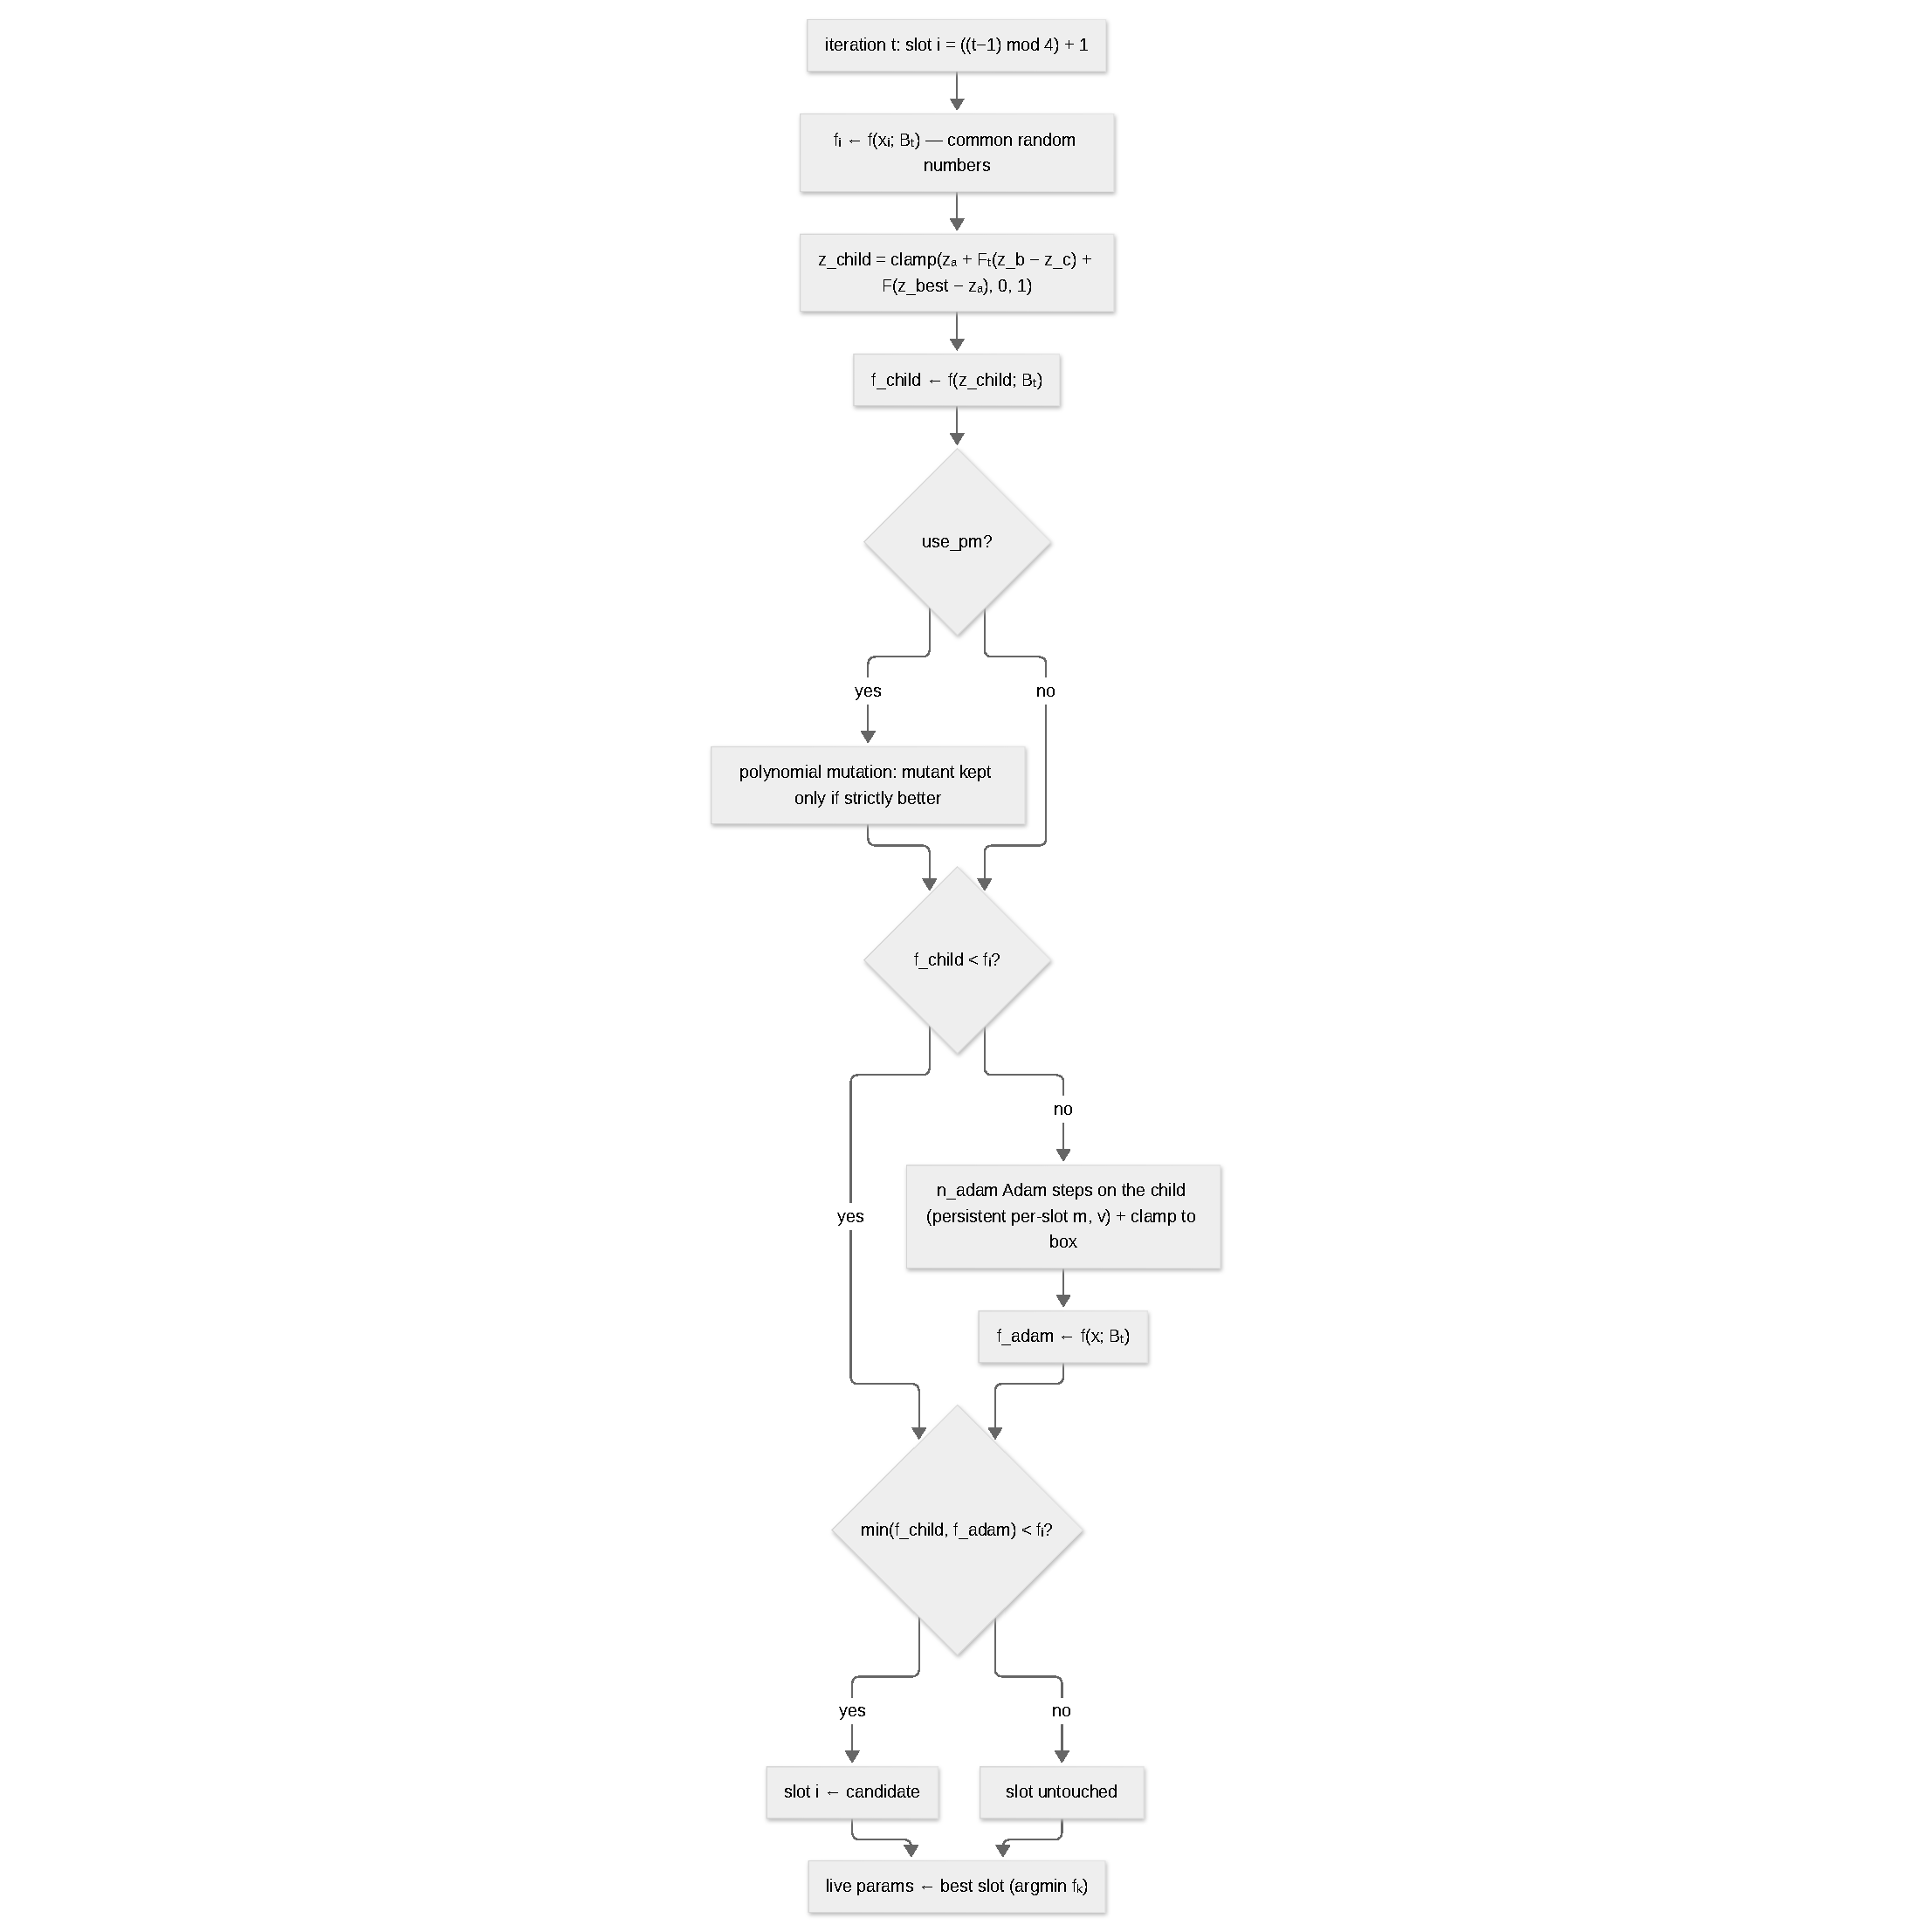
\includegraphics{figures/optimizers/eve.pdf}}
\caption{Step flow of EvE: a steady-state population of four challenges one round-robin slot per iteration with a DE child; a persistent-state Adam burst rescues the child only when it fails to improve, and greedy common-random-number selection keeps the best-so-far monotone.}
\label{fig:opt-eve}
\end{figure}
EvE~\citep{raj_eve_2026} is a \textbf{population-based alternate to Adam} targeted at the search-heavy, budget-constrained regime one level above final-stage training: ranking or pruning candidate configurations inside hyperparameter and architecture search. Instead of refining a single point, EvE keeps a steady-state population of four candidates and challenges one round-robin slot per iteration with a \emph{rand-to-pbest/1} differential-evolution child; only when the child fails to improve the slot's incumbent does EvE run a short burst of stock Adam on the same minibatch, keeping the refined point only if it beats the child. Selection is greedy, so the best-so-far value is monotone non-increasing on deterministic objectives, and because gradients are used only as a targeted rescue, per-iteration cost stays within a constant factor of a single Adam step regardless of dimension.

All internal search happens on the unit cube $z \in [0,1]^n$ via the affine map $\mathbf{x} = \mathbf{x}_l + \mathbf{z} \odot (\mathbf{x}_u - \mathbf{x}_l)$, so a fixed-size step never overshoots narrow-range coordinates or under-moves wide ones. The population is initialized by proximity — one anchor with three Gaussian jitters, $\sigma = 0.1$ — anchored at the model's own initial weights (the paper's LoRA precedent), with the per-tensor search box centered on the anchor at the Kaiming half-width $\sqrt{6/\mathrm{fan\_in}}$. Each iteration draws three distinct donors $a, b, c \ne i$ and builds the child with a jittered difference weight (the jitter applies only to the difference term; the pbest pull uses the unjittered $F$):
\begin{align}
z_{\text{child}} &= \operatorname{clamp}\big(z_a + F_t (z_b - z_c) + F (z_{\text{pbest}} - z_a),\ 0,\ 1\big), &
F_t &= F\big(1 + \gamma (u - \tfrac{1}{2})\big), \quad u \sim U(0,1),
\end{align}
with $F = 0.5$ and $\gamma = 10^{-4}$. An optional polynomial mutation (PM; off by default for neural-network training, since a single-coordinate nudge essentially never wins its accept/reject gate at network scale) perturbs exactly one gene at rate $p = 1/n$ with distribution index $\eta = 20$, the perturbation bounded and self-scaling to the distance to each boundary:
\begin{align}
z_d &\leftarrow z_d + \delta_q (z_u - z_l)_d, &
\delta_q &=
\begin{cases}
\bigl[2r + (1 - 2r)(1 - \delta_1)^{\frac{1}{\eta+1}}\bigr]^{\frac{1}{\eta+1}} - 1, & r \le 0.5,\\[2pt]
1 - \bigl[2(1 - r) + 2(r - 0.5)(1 - \delta_2)^{\frac{1}{\eta+1}}\bigr]^{\frac{1}{\eta+1}}, & r > 0.5,
\end{cases}
\end{align}
with $\delta_1 = (z_d - z_l)/(z_u - z_l)$, $\delta_2 = (z_u - z_d)/(z_u - z_l)$ and $r \sim U(0,1)$. When the (possibly mutated) child fails to beat the slot's value, EvE runs $n_{\text{adam}}$ stock-Adam steps on it \emph{in real coordinates}, with classic L2 weight decay folded into the gradient before the moment update (PyTorch's stock Adam, not AdamW's decoupled rule) and every iterate clamped back into the box:
\begin{align}
g_t &= \nabla_{\mathbf{x}} f(\mathbf{x}_{t-1}; B_t) + \lambda \mathbf{x}_{t-1}, &
m_t &= \beta_1 m_{t-1} + (1 - \beta_1) g_t, &
v_t &= \beta_2 v_{t-1} + (1 - \beta_2) g_t^2, \\
\widehat{m}_t &= \frac{m_t}{1 - \beta_1^t}, &
\widehat{v}_t &= \frac{v_t}{1 - \beta_2^t}, &
\mathbf{x}_t &= \operatorname{clamp}\Big(\mathbf{x}_{t-1} - \eta_{lr} \frac{\widehat{m}_t}{\sqrt{\widehat{v}_t} + \epsilon},\ \mathbf{x}_l,\ \mathbf{x}_u\Big),
\end{align}
with $\beta_1 = 0.9$, $\beta_2 = 0.999$, $\epsilon = 10^{-8}$. Each population slot keeps its own persistent $(m, v, t)$ state across the whole run, so fallback bursts form one continuous Adam trajectory rather than repeated cold starts. Every evaluation of an iteration — the slot refresh, the child and the whole fallback burst — is scored on one freshly drawn minibatch $B_t$ (common random numbers), and a candidate replaces the incumbent only if it is strictly better on that same batch. In this implementation the shared per-group \texttt{lr\_*}, \texttt{wd\_*}, \texttt{betas\_*} and \texttt{eps\_*} configure the Adam fallback per parameter group (\texttt{wd\_*} is the L2 term $\lambda$ inside $g_t$), the live model parameters always hold the best-so-far slot between steps, and the step is closure-based — the trainer re-evaluates the current batch on each candidate point inside \texttt{optimizer.step()}, which is why EvE requires \texttt{gradient\_accumulation\_steps: 1} and is not available for SBERT.

\begin{algorithm}[H]
\caption{EvE (Evolutionary Explorer)}
\label{alg:eve}
\begin{algorithmic}[1]
\Require Objective $f$ with bounds $\mathbf{x}_l, \mathbf{x}_u$, iterations $T$, DE weight $F$, jitter $\gamma$, init jitter $\sigma$, PM index $\eta$, fallback steps $n_{\text{adam}}$, fallback LR $\eta_{lr}$, L2 decay $\lambda$, seed $s$, USE\_PM
\Ensure Best point $\arg\min_k z_k$ and value $\min_k f_k$
\State $z_1 \sim U(0,1)^n$ (anchor: the initial weights); $z_k \gets \operatorname{clamp}(z_1 + \sigma\epsilon_k, 0, 1)$, $\epsilon_k \sim \mathcal{N}(0, I_n)$, $k = 2,3,4$ \Comment{Proximity init}
\State $f_k \gets f(\mathbf{x}_l + z_k \odot (\mathbf{x}_u - \mathbf{x}_l))$ for $k = 1,\dots,4$; $\text{state}_k \gets (\mathbf{0}, \mathbf{0}, 0)$ \Comment{Persistent Adam moments}
\For{$t = 1, \ldots, T$}
    \State $i \gets ((t - 1) \bmod 4) + 1$ \Comment{Round-robin target slot}
    \State draw minibatch $B_t$; $f_i \gets f(\mathbf{x}_i; B_t)$ \Comment{Common random numbers}
    \State draw distinct $a, b, c \in \{1,\dots,4\} \setminus \{i\}$; $F_t \gets F(1 + \gamma(u - 0.5))$, $u \sim U(0,1)$
    \State $z_{\text{child}} \gets \operatorname{clamp}(z_a + F_t(z_b - z_c) + F(z_{\text{pbest}} - z_a), 0, 1)$
    \State $f_{\text{child}} \gets f(z_{\text{child}}; B_t)$
    \If{USE\_PM} \Comment{PM's own accept/reject gate}
        \State $z_{\text{mut}} \gets \operatorname{PM}(z_{\text{child}}, \eta)$; $f_{\text{mut}} \gets f(z_{\text{mut}}; B_t)$
        \If{$f_{\text{mut}} < f_{\text{child}}$} $z_{\text{child}}, f_{\text{child}} \gets z_{\text{mut}}, f_{\text{mut}}$ \EndIf
    \EndIf
    \If{$f_{\text{child}} < f_i$}
        \State $z_{\text{cand}}, f_{\text{cand}} \gets z_{\text{child}}, f_{\text{child}}$
    \Else
        \State $\mathbf{x} \gets \mathbf{x}_l + z_{\text{child}} \odot (\mathbf{x}_u - \mathbf{x}_l)$
        \For{$n = 1, \ldots, n_{\text{adam}}$} \Comment{Targeted Adam fallback}
            \State $\mathbf{x} \gets \operatorname{AdamStep}(\mathbf{x}, \nabla_{\mathbf{x}} f(\mathbf{x}; B_t), \eta_{lr}, \lambda, \text{state}_i)$; \quad $\mathbf{x} \gets \operatorname{clamp}(\mathbf{x}, \mathbf{x}_l, \mathbf{x}_u)$
        \EndFor
        \State $z_{\text{adam}} \gets (\mathbf{x} - \mathbf{x}_l)/(\mathbf{x}_u - \mathbf{x}_l)$; \quad $f_{\text{adam}} \gets f(z_{\text{adam}}; B_t)$
        \State $(z_{\text{cand}}, f_{\text{cand}}) \gets \arg\min_{(z, f) \in \{(z_{\text{child}}, f_{\text{child}}),\, (z_{\text{adam}}, f_{\text{adam}})\}} f$
    \EndIf
    \If{$f_{\text{cand}} < f_i$} $z_i \gets z_{\text{cand}}$; \quad $f_i \gets f_{\text{cand}}$ \Comment{Greedy selection} \EndIf
\EndFor
\State \Return $\arg\min_k z_k$, $\min_k f_k$
\end{algorithmic}
\end{algorithm}

\paragraph{Cons.}
\begin{itemize}[leftmargin=*]
\item A step behind Adam at matched evaluation budgets: roughly one accuracy point on MNIST and 9--11\% higher relative test loss on the LoRA fine-tuning tasks; the paper does not claim final-stage superiority.
\item 13$\times$ the live parameter count in total storage (four population copies plus eight persistent moment copies) against Adam's 4$\times$; the measured peak GPU multiplier is lower (2.95$\times$) but fixed and dimension-independent.
\item The learning rate does not transfer from Adam's and needs its own search (3--100$\times$ higher depending on the task); the four-member population shows the widest seed-to-seed variance of the nine methods compared.
\item Closure-based step: the trainer re-evaluates the batch inside \texttt{optimizer.step()}, so gradient accumulation is unsupported and the SBERT loop (sentence-transformers \texttt{fit}) cannot host it; polynomial mutation is pure cost at network scale and is off by default.
\end{itemize}

\paragraph{Pros.}
\begin{itemize}[leftmargin=*]
\item Monotone best-so-far by construction on deterministic objectives (greedy accept-only-if-better selection), with per-iteration cost within a constant factor of a single Adam step regardless of dimension.
\item Wins or ties Adam on 76\% of 70 (problem, dimension) benchmark cells across seven classical scalable problems up to $10^6$ variables, most decisively on the multimodal ones.
\item Finishes matched evaluation budgets 1.7--3.9$\times$ faster in wall-clock on real training (an MLP on MNIST and LoRA fine-tuning of a 1.5B-parameter model), trading a modest amount of final quality for speed.
\item Inside successive halving, completes hyperparameter and architecture searches 3.1--3.5$\times$ faster while ranking candidate configurations about as consistently with Adam as Adam does with itself across seeds (Kendall's $\tau$ of 0.66--0.69).
\end{itemize}

\paragraph{EA4LLM (Evolution Strategies for Large Language Models).}
\begin{figure}[H]
\centering
\fitfigure{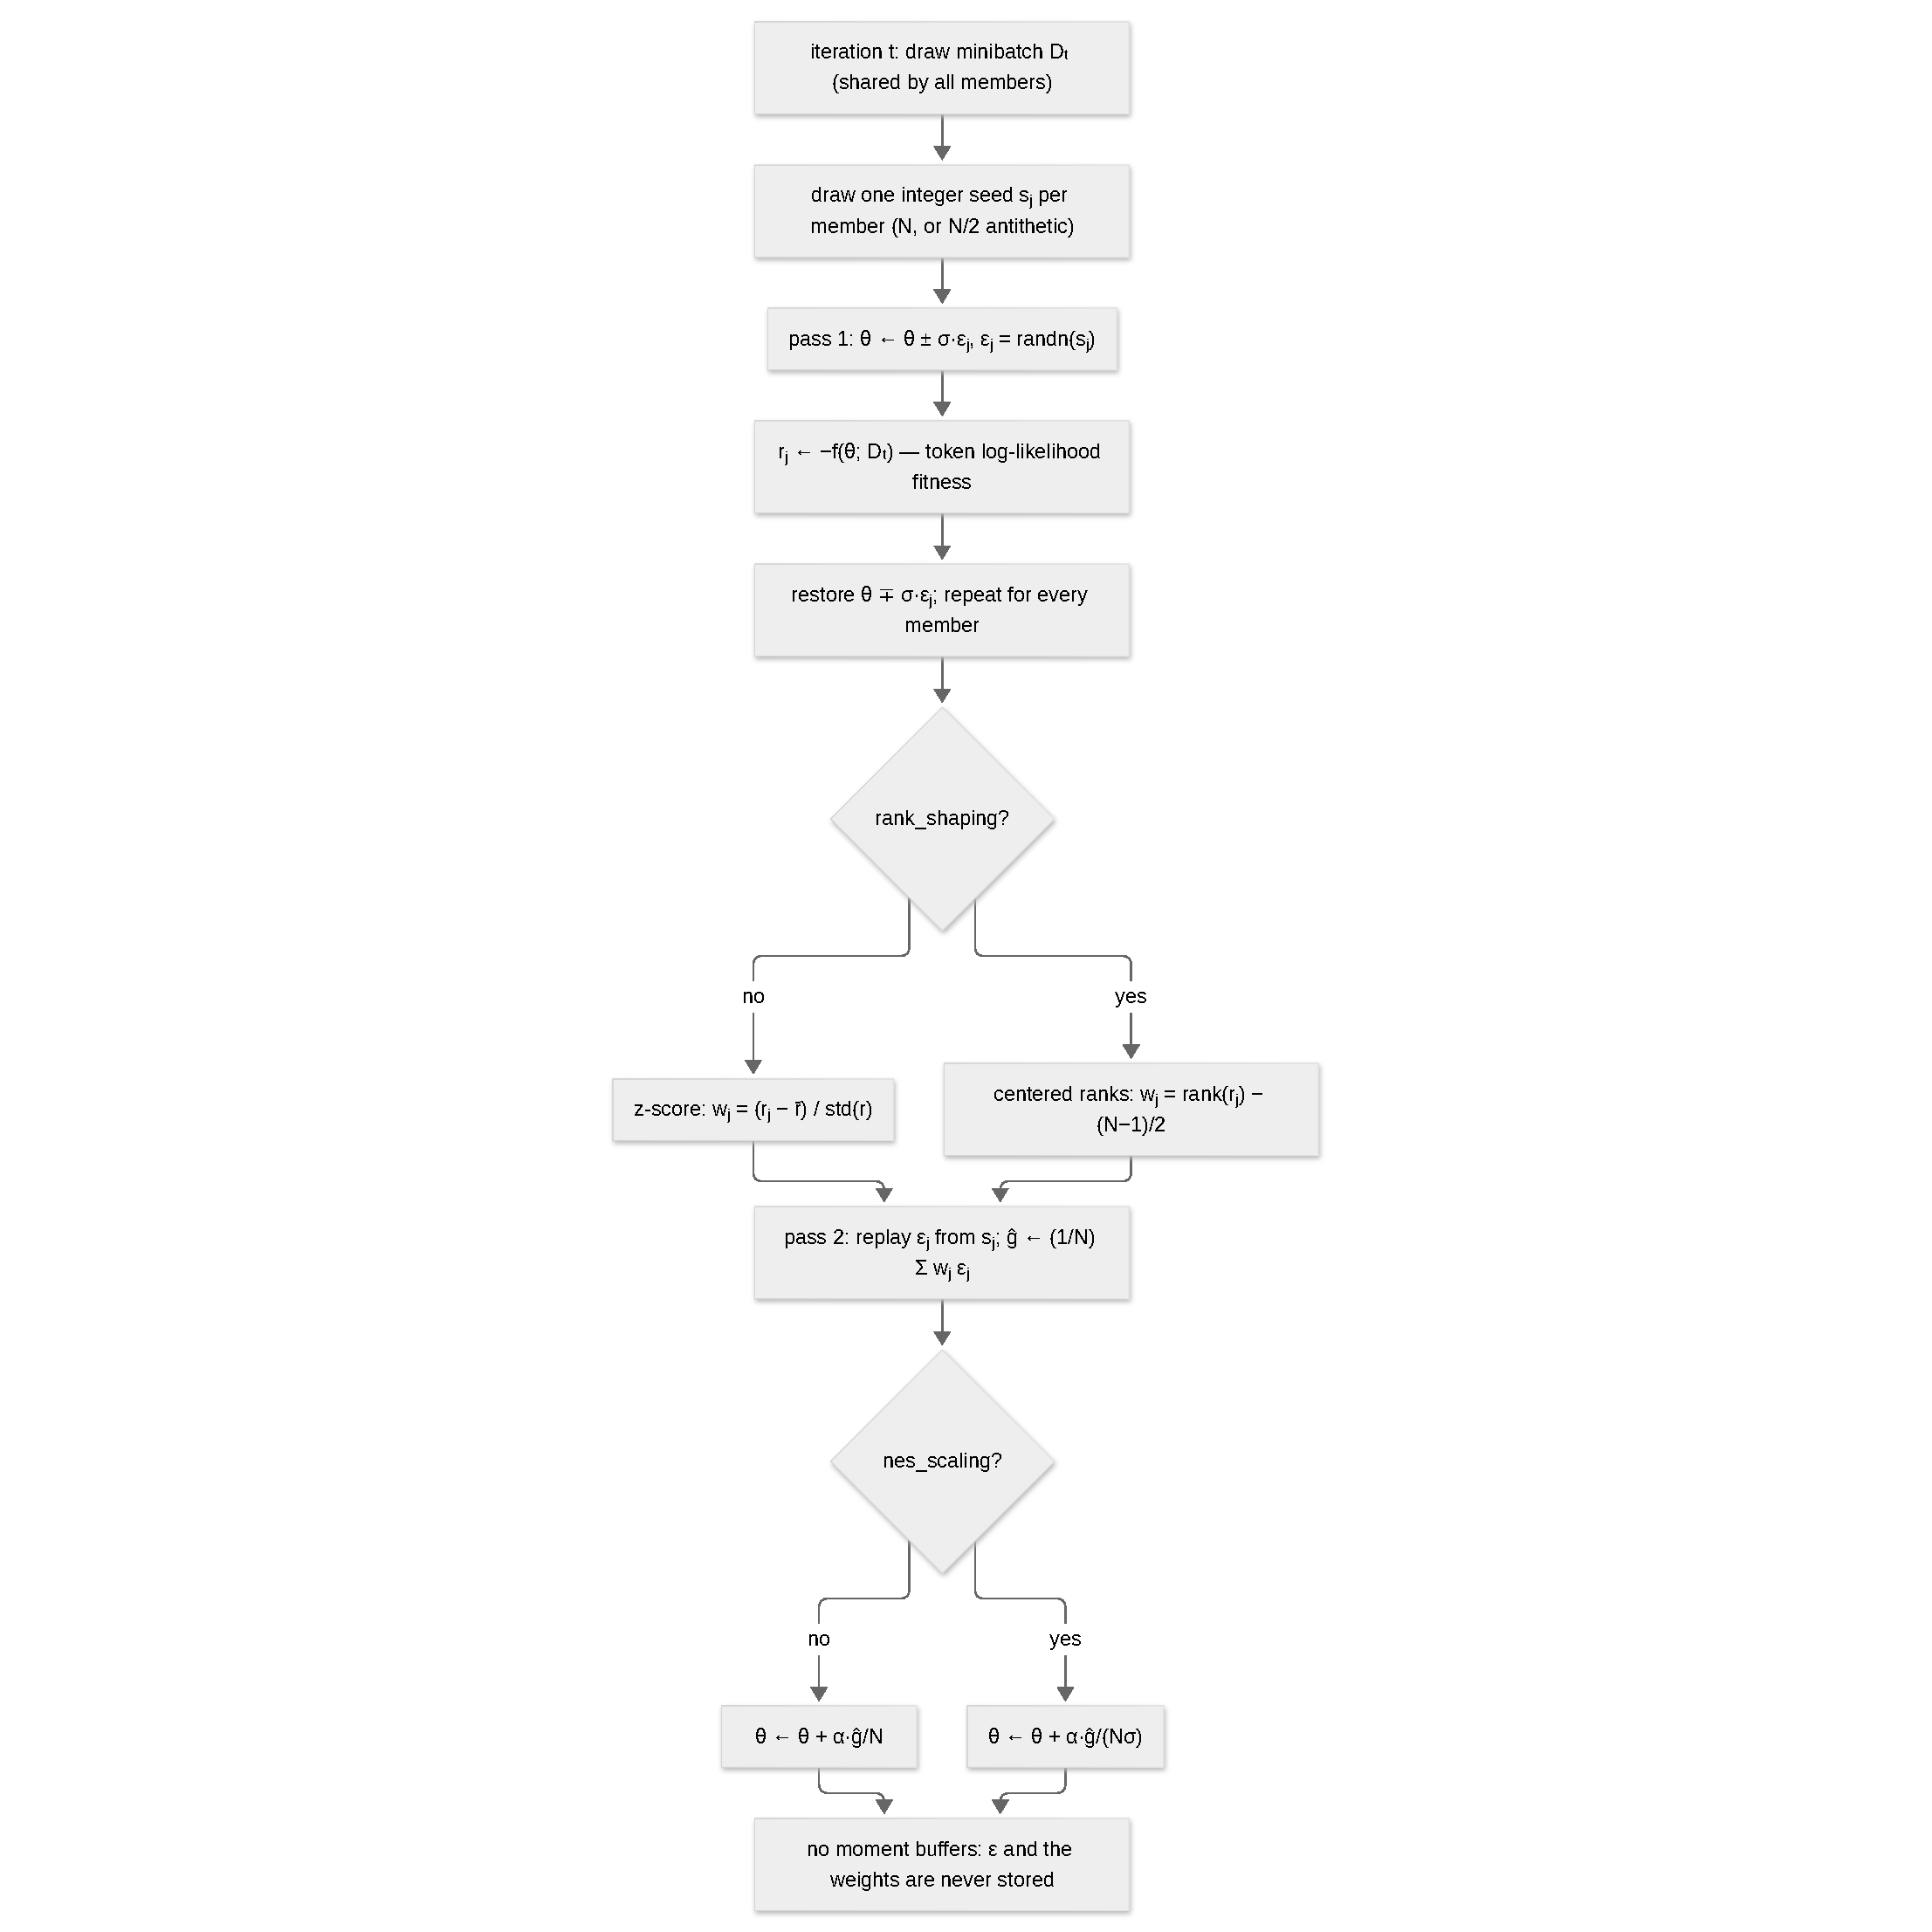
\includegraphics{figures/optimizers/ea4llm.pdf}}
\caption{Step flow of EA4LLM: each iteration evaluates $N$ Gaussian perturbations of the parameters on one minibatch shared by every member, scores them by the negated token-level log-likelihood, shapes the rewards into z-score or centered-rank weights, and replays the same seeded noise to accumulate the ES direction --- no gradients and no per-parameter optimizer state.}
\label{fig:opt-ea4llm}
\end{figure}
EA4LLM~\citep{liu_ea4llm_2025} is a \textbf{gradient-free alternative to Adam} that removes backpropagation and optimizer state entirely, and it is the first method the authors validate for full-parameter pretraining of LLMs from scratch, across Qwen3-style models from 0.5B to 32B parameters. Instead of differentiating a loss, EA4LLM treats the next-token likelihood as a black-box fitness and estimates a descent direction from a population of Gaussian perturbations. The fitness is the mean token-level log-probability of the true next token, masked for padding, which is exactly the standard causal-LM objective up to sign:
\begin{align}
p_t &= \operatorname{softmax}(z_t), &
R(x;\theta) &= \frac{1}{\sum_t m_t}\sum_{t=1}^{T} m_t \log p_\theta\!\left(x_{t+1}\mid x_{\le t}\right), &
F(\theta) &= \frac{1}{|D|}\sum_{x\in D} R(x;\theta),
\end{align}
with logits $z_t$, padding mask $m_t \in \{0,1\}$ and corpus $D$. Each iteration samples $N$ independent noises $\epsilon_j \sim \mathcal{N}(0, I)$, evaluates the perturbed fitness $r_j = F(\theta + \sigma\epsilon_j)$ on one uniformly drawn subset $D_t \subset D$ of size $M$ (the subset is shared by every member of the iteration, so the stochastic estimator stays unbiased, $\mathbb{E}[F_M(\theta)] = F(\theta)$), and shapes the rewards into weights by z-score normalization or centered ranks:
\begin{align}
w_j &= \frac{r_j - \bar r}{\operatorname{std}(r)}
&&\text{or}&
w_j &= \operatorname{rank}(r_j) - \frac{N-1}{2},
\end{align}
where $\operatorname{rank}(\cdot)$ assigns $0,\dots,N-1$ after sorting. The direction is the noise-weighted mean, optionally scaled NES-style by $1/\sigma$, and the update ascends the fitness:
\begin{align}
\hat g &= \frac{1}{N}\sum_{j=1}^{N} w_j \epsilon_j
&&\text{or}&
\hat g &= \frac{1}{N\sigma}\sum_{j=1}^{N} w_j \epsilon_j,
&&&
\theta \leftarrow \theta + \alpha \hat g .
\end{align}
Antithetic sampling evaluates the $\pm\sigma\epsilon$ pair of $N/2$ seeds instead of one sign per seed. The paper's runner uses $N = 30$, $\sigma = 10^{-3}$, $\alpha = 5\times 10^{-4}$ and $M = 5000$ evaluation samples per iteration ($T = 1000$ iterations, micro-batch 16, maximum sequence length 256); antithetic sampling, rank shaping, the NES $1/\sigma$ scaling, grouped/layered multipliers and step-size schedules are all \emph{off} in those runs, and Appendix~A.1 states that the deployed algorithm removes the grouped operators and multipliers outright. In this implementation the step is closure-based: the trainer's current minibatch supplies $D_t$ and the loss is negated to form the fitness, the shared per-group \texttt{lr\_*} is the step size $\alpha$, and \texttt{wd\_*} applies a decoupled multiplicative decay before the ES move (a repo-consistency extension --- the paper defines no weight decay). Noise is regenerated from one integer seed per member in a second pass, so the full noise set is never stored: optimizer state is O(1) and no moment buffers exist. Like EvE, EA4LLM requires \texttt{gradient\_accumulation\_steps: 1} and is not available for SBERT (the closure cannot coexist with the SBERT fit loop), and AMP is not supported on the closure path.

\begin{algorithm}[H]
\caption{EA4LLM (Zeroth-Order Evolution Strategies)}
\label{alg:ea4llm}
\begin{algorithmic}[1]
\Require Parameters $\theta$, fitness $F$ (negated loss), iterations $T$, population $N$, noise scale $\sigma$, step size $\alpha$, subset size $M$, normalization (z-score or rank), seed $s$, USE\_ANTITHETIC, USE\_RANK, USE\_NES
\Ensure Optimized parameters $\theta_T$
\State seed the persistent generator with $s$
\For{$t = 1, \ldots, T$}
    \State draw minibatch $D_t \subset D$, $|D_t| = M$ \Comment{Shared by all members}
    \State draw seeds $\{s_j\}_{j=1}^{N/2}$ (antithetic) or $\{s_j\}_{j=1}^{N}$
    \State $\text{rewards} \gets [\,]$ \Comment{Pass 1: perturb, evaluate, restore}
    \For{each seed $s_j$ and sign $\pm$ (or a single sign)}
        \State $\epsilon \gets \operatorname{randn}(s_j)$; \quad $\theta \gets \theta \pm \sigma\epsilon$; \quad $r \gets -f(\theta; D_t)$; \quad $\theta \gets \theta \mp \sigma\epsilon$
        \State append $r$ to rewards
    \EndFor
    \State $w \gets$ z-score(rewards) or centered ranks(rewards)
    \State $g \gets 0$ \Comment{Pass 2: replay the same noise}
    \For{each seed $s_j$ and sign $\pm$ (or a single sign)}
        \State $\epsilon \gets \operatorname{randn}(s_j)$; \quad $g \gets g + w_j (\pm\epsilon)$
    \EndFor
    \State $\theta \gets \theta + \alpha g / (N\sigma)$ if USE\_NES, else $\theta \gets \theta + \alpha g / N$
\EndFor
\State \Return $\theta_T$
\end{algorithmic}
\end{algorithm}

\paragraph{Cons.}
\begin{itemize}[leftmargin=*]
\item Requires $N$ forward evaluations per step (30 in the paper), so sample efficiency trails first-order methods and the variance of the estimate is higher; the paper reports sensitivity to $N$, $\sigma$, $\alpha$ and the normalization choice.
\item No gradient is available, so the gradient-clipping and AMP paths do not apply: the trainer's closure harness rejects \texttt{use\_amp}, requires \texttt{gradient\_accumulation\_steps: 1}, and the SBERT loop cannot host it. Each evaluation also pays a backward pass through the shared closure even though ES discards it.
\item At matched evaluation budgets the paper does not claim superior final quality to Adam; its case is memory (>4$\times$ reduction at $\ge$4B parameters) and gradient-free feasibility, with antithetic sampling, rank shaping and NES scaling disabled in its own large-scale runs.
\item Because the z-score makes the update magnitude independent of $\sigma$ and of the gradient scale, $\alpha$ must be tuned per task rather than transferred from Adam.
\end{itemize}

\paragraph{Pros.}
\begin{itemize}[leftmargin=*]
\item Zero optimizer state: no moments and no population copies, so the paper measures 60.01 vs 137.61~GB at 8B and 137.61 vs 431.76~GB at 32B against Adam.
\item Provides the first stable full-parameter ES pretraining from scratch across 0.5B--32B, with steadily decreasing loss curves (Figure~1) and no gradient computation.
\item Architecture-agnostic: the fitness only needs a forward pass and a probability, so non-differentiable operators become trainable.
\item The subsampled fitness is an unbiased estimator of the full-corpus fitness, and the two-pass seeded replay makes the noise reproducible while keeping optimizer state at O(1).
\end{itemize}


\small
\begin{longtable}{L{2.5cm}L{3.5cm}L{2.3cm}L{5.0cm}}
\toprule
\textbf{Group} & \textbf{Methods} & \textbf{Primary Goal} & \textbf{Interpretation from the Survey} \\
\midrule
\endhead
Classical baseline & SGD, SGD with momentum, RMSProp, AdamW, RAdam & stability and reference baselines & These define the comparison floor for newer optimizer claims. \\
Momentum redesign & Adan, AdEMAMix, MARS, Cautious AdamW & faster or safer first-order adaptation & Best when convergence speed or noisy-gradient stability is the main concern. \\
Large-batch and schedule simplification & LAMB, Schedule-Free AdamW & operational robustness at scale & Reduce brittleness from batch-size growth or schedule engineering. \\
Memory-efficient & Adafactor, GaLore, APOLLO, APOLLO-Mini, Q-APOLLO, Lion & optimizer-state reduction & Most useful when VRAM is dominated by optimizer state rather than activations; APOLLO-family methods replace dense AdamW moments with projected or quantized structured scaling. \\
Curvature-aware & Shampoo, SOAP, Sophia & better conditioning & Prefer when richer geometry is worth implementation and compute overhead. \\
Geometry-oriented & Muon, Turbo-Muon, AF-Muon, AdaMuon, Dion3 & orthogonalized update structure & Specialized options for matrix geometry and representation shaping; AdaMuon adds an element-wise second moment on the orthogonalized direction with RMS-aligned updates; AF-Muon assigns the tied vocabulary table a capped-row table geometry and one-dimensional parameters an RMS update, with no AdamW auxiliary state; Dion3 keeps the spectral update but orthogonalizes only a fraction of the momentum rows per step with Gram Newton--Schulz and error feedback. \\
Evolutionary hybrid & EvE, EA4LLM & fast, monotone candidate ranking for search loops; gradient-free full-parameter updates & A steady-state differential-evolution population with a targeted Adam rescue trades final quality for wall-clock speed; best used as the inner optimizer of hyperparameter or architecture search. EA4LLM removes gradients entirely --- zeroth-order ES with token-level log-likelihood fitness and no optimizer state, the memory-first option for pretraining at scale. \\
\bottomrule
\end{longtable}
\normalsize

